\documentclass[twoside,openright,bibliography=totoc]{scrreprt}
%\documentclass[report,mono,twoside,openright]{tugrazbooklet}
%\documentclass[a4paper]{book}

\usepackage[phd]{tugrazthesis}
% options:
%   - msc (for Master's thesis/Masterarbeit) OR
%     diplom (for Diploma thesis/Diplomarbeit) OR
%     phd (for Doctoral thesis/Dissertation)
%   - nawi (for NAWI curricula)
%   - individual (for Individuelles Masterstudium)

\usepackage[ngerman,english]{babel}  % uncomment to switch to German

%\usepackage{filecontents}  % for the integrated bibliography file (backwards compatibility)
%\usepackage[backend=backend,style=numeric-comp]{biblatex}  % to generate the bibliography
%\addbibresource{phd-missethan.bib}  % name of the bib-file

%---Packages-Introduction---------------------------------------------------------------

\usepackage[sort]{cite}
\usepackage{amsmath,amssymb,amsthm}
\definecolor{colourCite}{RGB}{50,128,50}
\definecolor{colourLink}{RGB}{200,0,0}
\usepackage[citebordercolor=colourCite,linkbordercolor=colourLink]{hyperref}
\usepackage[capitalize, noabbrev]{cleveref}


% ---------------- Theorem environments ---------------------------------

\newtheorem{theorem}{Theorem}[section]
\newtheorem{proposition}[theorem]{Proposition}
\newtheorem{corollary}[theorem]{Corollary}
\newtheorem{lemma}[theorem]{Lemma}
\newtheorem{observation}[theorem]{Observation}
\newtheorem{conjecture}[theorem]{Conjecture}
\newtheorem{prob}{Problem}[]
\theoremstyle{definition} 
\newtheorem{definition}[theorem]{Definition}
\newtheorem{example}[theorem]{Example}
\newtheorem{question}[theorem]{Question}

\crefname{theorem}{theorem}{theorems}
\crefname{proposition}{proposition}{propositions}
\crefname{corollary}{corollary}{corollaries}
\crefname{lemma}{lemma}{lemmas}
\crefname{definition}{definition}{definitions}
\crefname{conjecture}{conjecture}{conjectures}


%--------------- Chapter 1. Recoverable Selection
%\usepackage{natbib}
%\usepackage{etex}
%\usepackage{scrhack}
%\usepackage{cmap}
%\usepackage[ngerman,english]{babel}
\usepackage[utf8]{inputenc}
\usepackage{graphicx}
\usepackage{caption}
\usepackage{subfigure}
%\usepackage{epstopdf}
\usepackage{mathtools}
%\usepackage{amsmath}
%\usepackage{amsthm}
%\usepackage{amssymb}
%\usepackage{comment}
\usepackage{multirow}
\usepackage{tikz}
%\usetikzlibrary{arrows,intersections}
%\usetikzlibrary{shapes}
%\usepackage[english,vlined,ruled]{algorithm2e}
\usepackage{hyperref}
\usepackage{lipsum}
\usepackage{float}
\usepackage{tabularx}
%\usepackage{booktabs}
%\usepackage{longtable}
%\usepackage{tabu}
%\usepackage{environ}
%\usepackage{mdframed}
%\usepackage{datetime}
\usepackage{enumerate}
%\usepackage{authblk}

%%------------------------ Chapter 3. Interval Interdiction
%\usepackage{amsmath}
%\usepackage{amsfonts}
%\usepackage{amssymb}
\usepackage{authblk}

%\usepackage{graphicx}
%\usepackage{hyperref}
%\usepackage[capitalize, noabbrev]{cleveref}
\usepackage[autostyle=true]{csquotes}
\usepackage{color}
\usepackage{multirow}
%algorithm package
\usepackage[ruled, lined, linesnumbered, commentsnumbered, noend]{algorithm2e}
%packages used for subfigures
%\usepackage{caption}
%\usepackage{subcaption}

%%--------------------------- Chapter 5. Linearization 2

%\usepackage[utf8]{inputenc}
%\usepackage{amsmath}
%\usepackage{amsfonts}
%\usepackage{amssymb}
%\usepackage{authblk}
\usepackage{verbatim}
\usepackage{thmtools}
%\usepackage{amsthm}
\usepackage{thm-restate}
\usepackage{todonotes}
%\declaretheorem[name=Theorem,numberwithin=section]{thm}
%--experiment
%\usepackage%[hidelinks]{hyperref}

%\usepackage[capitalize, noabbrev]{cleveref}
%\usepackage[autostyle=true]{csquotes}
%\usepackage{graphicx}
%\usepackage{color}
%\usepackage{enumerate}
%\usepackage[ruled, lined, linesnumbered, commentsnumbered, noend]{algorithm2e}

%\usepackage{tikz}
\usetikzlibrary{calc}
\usetikzlibrary{arrows,shapes}
\usetikzlibrary{decorations.markings}
\usetikzlibrary{arrows.meta}

%------------------------ Chapter 6. Nonpreemptive Tree Packing

%\usepackage[utf8]{inputenc}
%\usepackage{amsmath,amsfonts,amssymb}
%\usepackage{thmtools}
%\usepackage{amsthm}
%\usepackage{thm-restate}

%\usepackage{hyperref}
%\usepackage[capitalize, noabbrev]{cleveref}
%\usepackage{graphicx}
%\usepackage{color}
%\usepackage{enumerate}
%\usepackage{caption}
%\usepackage{subcaption}
\usepackage{array}
%\usepackage{authblk}

\usepackage{tikz,tikzsymbols}
\usetikzlibrary{shapes,patterns,positioning}
\usetikzlibrary{arrows,decorations.markings}
\usetikzlibrary{calc}


%\makeatletter
%\renewcommand{\@pnumwidth}{3em} 
%\renewcommand{\@tocrmarg}{4em}
%\makeatother

\overfullrule=3mm

%---Macros-Universal---------------------------------------------------------------
\newcommand{\R}{\mathbb{R}}
\newcommand{\N}{\mathbb{N}}
\newcommand{\Z}{\mathbb{Z}}
\newcommand{\set}[1]{\{ #1 \}}
\newcommand{\fromto}[2]{\set{#1, \ldots, #2}}

\newcommand{\rz}{\mathbb{R}}
\newcommand{\nz}{\mathbb{Z}}


\newcommand{\bigO}{\mathcal{O}}
\newcommand{\dotunion}{\mathbin{\dot{\cup}}}
\newcommand{\powerset}{\mathcal{P}}



%---------- Chapter 1. Recoverable Selection -------------
\newcommand{\bigM}{\Omega}
\newcommand{\ra}{\rightarrow}
\newcommand{\la}{\leftarrow}
\newcommand{\Ra}{\Rightarrow}
\newcommand{\La}{\Leftarrow}
\newcommand{\sgn}{\operatorname{sgn}}
\newcommand{\out}{\operatorname{out}}
\newcommand{\inn}{\operatorname{in}}
\newcommand{\val}{\operatorname{val}}
\newcommand{\head}{\operatorname{head}}
\newcommand{\tail}{\operatorname{tail}}
\newcommand{\rev}{\operatorname{rev}}
\newcommand{\ord}{\operatorname{ord}}
\newcommand{\prev}{\operatorname{prev}}
\newcommand{\first}{\operatorname{first}}
\newcommand{\last}{\operatorname{last}}
\newcommand{\oleft}{\operatorname{left}}
\newcommand{\aux}{\operatorname{aux}}
\newcommand{\mh}{displaymath}
\newcommand{\nn}{\mathbb{N}}
\newcommand{\nnz}{\mathbb{N}_0}
\newcommand{\qq}{\mathbb{Q}}
\newcommand{\zz}{\mathbb{Z}}
\newcommand{\rr}{\mathbb{R}}
\newcommand{\kk}{\mathbb{K}}
\newcommand{\cc}{\mathbb{C}}
\newcommand{\ff}{\mathbb{F}}
\newcommand{\pp}{\mathcal{P}}
\newcommand{\eps}{\epsilon}
\newcommand{\Lra}{\Leftrightarrow}
\newcommand{\mbf}[1]{\text{\textbf{#1}}}
\newcommand{\udot}{\mathbin{\dot{\cup}}}
\newcommand{\bigudot}{\mathop{\dot{\bigcup}}}
\newcommand{\vek}[1]{\boldsymbol{#1}}
\newcommand{\id}{\operatorname{id}}
\newcommand{\poly}{\operatorname{poly}}
\newcommand{\scalp}[2]{{#1}^{t} {#2}}
\newcommand{\method}[1]{\texttt{#1}}
\newcommand{\opt}{\mathit{OPT}}
\newcommand{\alg}{\mathit{ALG}}
\newcommand{\rank}{\operatorname{rk}}
\newcommand{\probl}[1]{\textsc{#1}}
\newcommand{\matroid}{\mathcal{M}}
\newcommand{\base}{E}
\newcommand{\basis}{\mathcal{B}}
\newcommand{\inds}{\mathcal{F}}
\newcommand{\transit}{\tau}
\newcommand{\myc}{c}
\newcommand{\myd}{\bar{c}}
\newcommand{\scenset}{\mathcal{U}}
\newcommand{\lowcost}{\underline{c}}
\newcommand{\upcost}{\bar{c}}
\newcommand{\fscost}{C}

\newcommand{\X}{\mathcal{X}}
\newcommand{\cU}{\mathcal{U}}

\newcommand{\fillfield}[2]{\draw[fill=lightgray]  (#1-1,#2-1,0) -- (#1-1,#2,0) -- (#1,#2,0) -- (#1,#2-1,0) -- cycle;}
\newcommand{\fillfieldr}[2]{ \draw[step=1,thick, red] (#1-1,#2-1) grid (#1,#2); }
\newcommand{\fillfieldg}[2]{ \draw[step=1,thick, blue] (#1-1,#2-1) grid (#1,#2); }

% names
\newcommand{\ptime}[2]{p^{(#1)}_{#2}}
\newcommand{\plow}[1]{p^{-}_{#1}}
\newcommand{\pup}[1]{p^{+}_{#1}}
\newcommand{\ctime}[2]{C^{(#1)}_{#2}}

\newcommand{\lasse}[1]{{#1}}

\DeclareMathOperator*{\argmax}{\arg\!\max}
\DeclareMathOperator*{\argmin}{\arg\!\min}

\DeclarePairedDelimiter{\ceil}{\lceil}{\rceil}
\DeclarePairedDelimiter{\floor}{\lfloor}{\rfloor}
\DeclarePairedDelimiter{\abs}{\lvert}{\rvert}


%------------ Chapter 2. Multistage Complexity

\newcommand{\new}[1]{#1}
%\newcommand{\X}{{\mathcal{X}}}
%\newcommand{\cU}{{\mathcal{U}}}
\newcommand{\cI}{{\mathcal{I}}}
\newcommand{\cC}{{\mathcal{C}}}
\newcommand{\cB}{{\mathcal{B}}}
%\newcommand{\rev}[1]{\textcolor{blue}{#1}} %text segments changed in the revision
%\newcommand{\R}{\mathbb{R}}
%\newcommand{\N}{\mathbb{N}}

\newcommand{\radj}{R-Adj-SAT}

\newcommand{\unc}{\mathcal{Z}}

%\newcommand{\set}[1]{\{ #1 \}}
%\newcommand{\fromto}[2]{\set{#1,\dots,#2}}

%------------ chapter 3. Interval Interdiction

\newcommand{\True}{\textsc{True}}
\newcommand{\False}{\textsc{False}}

%\newcommand{\comment}[1]{\textcolor{red}{(#1)}}

\newcommand{\las}[1]{#1}

\newcommand{\hun}[1]{#1}

\DeclareMathOperator{\ac}{\text{A}}
%\DeclareMathOperator{\val}{\text{value}}
\DeclareMathOperator{\dist}{\text{dist}}
\DeclareMathOperator{\rel}{\text{rel}}
\DeclareMathOperator{\betw}{\text{betw}}
\DeclareMathOperator{\valid}{\text{valid}}
\DeclareMathOperator{\cost}{\text{cost}}



%Special short commands for interval interdiction notation
\newcommand{\I}{\mathcal{I}}
\newcommand{\J}{\mathcal{J}}
\newcommand{\F}{\mathcal{F}}
\DeclareMathOperator{\graph}{G}

\newcommand{\claimqed}{\hfill\scriptsize$\blacksquare$\normalsize}

%---------------- Chapter 4. Linearization 1

%\newcommand{\proof}{\emph{Proof.}\ \ }
%\newcommand{\qed}{~~$\Box$}
\newcommand{\RRR}{{\mathbb{R}_{\ge0}}}

\newcommand{\spp}{\text{SPP}}
\newcommand{\qspp}{\text{QSPP}}
\newcommand{\ppp}{{\cal P}_{st}}
\newcommand{\pppx}{{\cal P}^+}
\newcommand{\pppy}{{\cal P}^-}

\newcommand{\boxxx}[1]
 {\fbox{\begin{minipage}{13.00cm}\begin{center}\bigskip\begin{minipage}{12.30cm}
  #1\end{minipage}\end{center}~\end{minipage}}}

%---------------- Chapter 5. Linearization 2


\newcommand{\const}{\textsf{source}}
%\newcommand{\ren}[1]{{\color{magenta}{#1}}}

\newcommand{\Pst}{\mathcal{P}_{st}}
\newcommand{\Nscript}{N}

%\newcommand{\boxxx}[1]
% {\fbox{\begin{minipage}{11.80cm}\begin{center}\bigskip\begin{minipage}{11.30cm}
%  #1\end{minipage}\end{center}~\end{minipage}}}

\DeclareMathOperator{\red}{\textsf{reduced}}
\DeclareMathOperator{\xval}{val}

%----------------------- Chapter 6. NTP

\newcommand{\RR}{\mathbb{R}}
\newcommand{\NN}{\mathbb{N}}
\newcommand{\ZZ}{\mathbb{Z}}

%\newcommand{\comment}[1]{\textcolor{red}{(L: #1)}}

\newcommand{\xxxNTP}{\textsc{N-TreePack}}
\newcommand{\xxxHAM}{\textsc{Hamilton-3-reg}}
\DeclareMathOperator{\ntp}{\textsf{ntp}}
\newcommand{\greedy}{\textsf{Greedy}}

%\newcommand{\lasse}[1]{\textcolor{blue}{#1}}
%\newcommand{\lasse}[1]{#1}


\begin{document}
%--- INFORMATION FOR TITLEPAGE -------------------------------------------------

% Your name including previous academic degrees (optional argument sets a different \author{}):
\thesisauthor[Lasse Wulf]{Lasse Wulf, B.Sc. M.Sc. M.Sc.}

% Title of your thesis (optional argument sets a different \title{}):
\thesistitle[Random planar graphs]{On generalizations of some classical combinatorial optimization problems.\\ Multi-stage robustness, higher-order cost functions, and nonpreemption.}

% Date of completion (optional argument sets a different \date{})
\thesisdate[ ]{July 2023}

% Supervisor headline (select male/female/plural version)
\supervisortitle{\germanenglish{Betreuerin}{Supervisor}}

% Supervisor info
\supervisor{%
  Univ.-Prof. Bettina Klinz, Ph.D.
\\[0.7cm]
  Institute of Discrete Mathematics

  %optional extra information (second advisor, name of faculty, etc.)\\
  %up to 2 lines
}

% Academic degree achieved with this thesis, according to your curriculum (check curriculum and select male/female version):
\academicdegree{Doktor der technischen Wissenschaften} % phd


%--- FRONT MATTER --------------------------------------------------------------
\pagenumbering{gobble}


% Insert title page and affidavit

\printthesistitle

\printaffidavit

% Other front matter you may want to include

\pagenumbering{roman}

\chapter*{Abstract}

English Abstract

\begin{otherlanguage}{ngerman}
\chapter*{Kurzfassung}
Deutscher Abstract
\end{otherlanguage}



% You will typically include *both a German and an English abstract*.
% The rest of the document will be either in German or in English.

\cleardoublepage

\chapter*{\germanenglish{Danksagung}{Acknowledgements}}

Acknowledgements.

\cleardoublepage

\setcounter{tocdepth}{1}
\tableofcontents



%--- MAIN CONTENT --------------------------------------------------------------

%\pagenumbering{arabic}

\pagenumbering{arabic}
\chapter{Introduction}
Less than 80 years after the invention of the first computer, today we are surrounded by digital technology at every step we make. 
Computers influence and control a huge amount of aspects of modern life. 
We have grown so accustomed to computers, that we take many of their wonderous abilities for granted. 
One of these magical abilities is to find the optimal solution to a problem out of an incredibly large amount of possibilities.
For example, suppose you wanted to go from Paris to Berlin by car. There is an almost infinite amount of different paths from Paris to Berlin. Yet, a clever computer algorithm can select the single unique path which is the fastest among all of them.

This ability of computers to find the optimal solution for a given problem is used in many areas of today's live: Computers are used to find the cheapest flight schedule for an airline, to find the best investment scheme for a portfolio, to decide which taxis from a taxi company should pick up which customer, to design optimal communication networks, and many, many more problems. Application areas range from Economics, Logistics, Operations Research, Computer Science, Healthcare, Biology, and many other disciplines.

It is important to state that computers do not come with this ability a priori. Instead, specific programs and algorithms need to be developed, to be able to handle the huge amount of possibilities. 
\emph{Combinatorial Optimization} is the scientific field concerned with the question: How do we pick the optimal solution out of a huge (but still finite) amount of possibilities? 
In particular, Combinatorial Optimization tries to understand, what all the previously listed problems have in common, and tries to develop a mathematical theory of these problems and the tools to solve them. Classically, Combinatorial Optimization tries to classify problems as either being intractable (NP-hard) or tractable (polynomial-time solvable). For the intractable problems, it tries to understand what exactly makes them intractable, and whether we can find at least approximate, almost-optimal solutions.

The area of Combinatorial Optimization lies in the intersection between discrete mathematics and theoretical computer science. 
Just like the computer, it is a relatively new scientific field (at least compared to other ares of mathematics). In this thesis, we are concerned 

\section{Motivation and background}
Very motivating.



%\usepackage[margin=25mm]{geometry}


% theorem environments
%\newtheorem{theorem}{Theorem}%[section]
%\newtheorem{cor}{Corollary} %[section]
%\newtheorem{lem}{Lemma}%[section]
%\newtheorem{obs}{Observation}%[section]
%\newtheorem*{prop}{Proposition} %[section]
%\newtheorem{prob}{Problem}[]
%\newtheorem*{question}{Question}

%\theoremstyle{definition}
%\newtheorem*{defi}{Definition} %[section]
%\newtheorem*{nota}{Notation} %[section]
%\newtheorem{algo}{Algorithmus} %[section]

%\theoremstyle{remark}
%\newtheorem*{rem}{Remark}
%\newtheorem*{ex}{Example}


%\newenvironment{claim}[1]{\par\medskip\noindent\underline{Claim:}\space#1}{}
%\newenvironment{claimproof}[1]{\par\medskip\noindent\underline{Proof:}\space#1}{\hfill
%$\diamond$}

%
%\mdfdefinestyle{probframe}{skipabove=0pt,skipbelow=0pt,innerleftmargin=0pt,
%innerrightmargin=5pt,innertopmargin=0pt, innerbottommargin=5pt}

%\makeatletter
%\newcommand{\problemtitle}[1]{\gdef\@problemtitle{#1}}% Store problem title
%\newcommand{\probleminput}[1]{\gdef\@probleminput{#1}}% Store problem input
%\newcommand{\problemquestion}[1]{\gdef\@problemquestion{#1}}% Store problem question
%\NewEnviron{problem}{
%    \medskip
%\begin{mdframed}[style=probframe]
%  \problemtitle{}\probleminput{}\problemquestion{}% Default input is empty
%  \BODY% Parse input
%  \par\addvspace{.5\baselineskip}
%  \noindent
%  \begin{tabularx}{\textwidth}{@{\hspace{\parindent}} l X c}
%    \multicolumn{2}{@{\hspace{\parindent}}l}{\@problemtitle} \\% Title
%    \textbf{Input:} & \@probleminput \\% Input
%    \textbf{Question:} & \@problemquestion% Question
%  \end{tabularx}
%  \par\addvspace{.5\baselineskip}
%\end{mdframed}
%    \medskip
%}
%\makeatother

% macros
%\newcommand{\bigM}{\Omega}
%\newcommand{\ra}{\rightarrow}
%\newcommand{\la}{\leftarrow}
%\newcommand{\Ra}{\Rightarrow}
%\newcommand{\La}{\Leftarrow}
%\newcommand{\sgn}{\operatorname{sgn}}
%\newcommand{\out}{\operatorname{out}}
%\newcommand{\inn}{\operatorname{in}}
%\newcommand{\val}{\operatorname{val}}
%\newcommand{\head}{\operatorname{head}}
%\newcommand{\tail}{\operatorname{tail}}
%\newcommand{\rev}{\operatorname{rev}}
%\newcommand{\ord}{\operatorname{ord}}
%\newcommand{\prev}{\operatorname{prev}}
%\newcommand{\first}{\operatorname{first}}
%\newcommand{\last}{\operatorname{last}}
%\newcommand{\oleft}{\operatorname{left}}
%\newcommand{\aux}{\operatorname{aux}}
%\newcommand{\mh}{displaymath}
%\newcommand{\nn}{\mathbb{N}}
%\newcommand{\nnz}{\mathbb{N}_0}
%\newcommand{\qq}{\mathbb{Q}}
%\newcommand{\zz}{\mathbb{Z}}
%\newcommand{\rr}{\mathbb{R}}
%\newcommand{\kk}{\mathbb{K}}
%\newcommand{\cc}{\mathbb{C}}
%\newcommand{\ff}{\mathbb{F}}
%\newcommand{\pp}{\mathcal{P}}
%\newcommand{\eps}{\epsilon}
%\newcommand{\Lra}{\Leftrightarrow}
%\newcommand{\mbf}[1]{\text{\textbf{#1}}}
%\newcommand{\udot}{\mathbin{\dot{\cup}}}
%\newcommand{\bigudot}{\mathop{\dot{\bigcup}}}
%\newcommand{\vek}[1]{\boldsymbol{#1}}
%\newcommand{\id}{\operatorname{id}}
%\newcommand{\poly}{\operatorname{poly}}
%\newcommand{\scalp}[2]{{#1}^{t} {#2}}
%\newcommand{\method}[1]{\texttt{#1}}
%\newcommand{\opt}{\mathit{OPT}}
%\newcommand{\alg}{\mathit{ALG}}
%\newcommand{\rank}{\operatorname{rk}}
%\newcommand{\probl}[1]{\textsc{#1}}
%\newcommand{\matroid}{\mathcal{M}}
%\newcommand{\base}{E}
%\newcommand{\basis}{\mathcal{B}}
%\newcommand{\inds}{\mathcal{F}}
%\newcommand{\transit}{\tau}
%\newcommand{\myc}{c}
%\newcommand{\myd}{\bar{c}}
%\newcommand{\scenset}{\mathcal{U}}
%\newcommand{\lowcost}{\underline{c}}
%\newcommand{\upcost}{\bar{c}}
%\newcommand{\fscost}{C}
%
%\newcommand{\X}{\mathcal{X}}
%\newcommand{\cU}{\mathcal{U}}
%
%\newcommand{\fillfield}[2]{\draw[fill=lightgray]  (#1-1,#2-1,0) -- (#1-1,#2,0) -- (#1,#2,0) -- (#1,#2-1,0) -- cycle;}
%\newcommand{\fillfieldr}[2]{ \draw[step=1,thick, red] (#1-1,#2-1) grid (#1,#2); }
%\newcommand{\fillfieldg}[2]{ \draw[step=1,thick, blue] (#1-1,#2-1) grid (#1,#2); }
%
%
%
%% names
%\newcommand{\ptime}[2]{p^{(#1)}_{#2}}
%\newcommand{\plow}[1]{p^{-}_{#1}}
%\newcommand{\pup}[1]{p^{+}_{#1}}
%\newcommand{\ctime}[2]{C^{(#1)}_{#2}}
%
%\newcommand{\lasse}[1]{\textcolor{red}{#1}}
%
%\DeclareMathOperator*{\argmax}{\arg\!\max}
%\DeclareMathOperator*{\argmin}{\arg\!\min}
%
%\DeclarePairedDelimiter{\ceil}{\lceil}{\rceil}
%\DeclarePairedDelimiter{\floor}{\lfloor}{\rfloor}
%\DeclarePairedDelimiter{\abs}{\lvert}{\rvert}

\chapter{Recoverable Representative Selection with Discrete Budgeted Uncertainty}
\label{ch:recov-selection}

\section{Introduction}\label{sec:intro}


Most optimization problems in practice are uncertain. To handle such problems under uncertainty, a vibrant field of research has been developed, including such approaches as fuzzy optimization (see e.g. \cite{lodwick2010fuzzy,klir1995fuzzy}), the stability approach (see e.g. \cite{sotskov2014sequencing}), stochastic programming (see e.g. \cite{birge2011introduction}), or robust optimization (see e.g. \cite{kasperski2016robust}). Treating uncertainty in an optimization problem typically increases its computational complexity, which means that a problem that is simple under known problem data may become challenging when the data is not known precisely.

In this paper we consider one such problem, which is the representatives multi-selection problem (RMSP). We are given several disjoint sets of items, and need to choose a specified number of items from each set. The aim is to minimize a linear cost function. Due to their simplicity, selection problems arise as special cases of many other fundamental combinatorial optimization problems, see \cite{kasperski2013approximating} for an overview. These include knapsack, assignment, scheduling, matroid base, spanning tree and shortest path problems. Choosing representative subsets in the widest sense also occurs, e.g., in data mining \cite{daszykowski2002representative,wang2017representative}, computer vision \cite{meng2016keyframes}, multi-objective optimization \cite{zio2011clustering}, or signal processing \cite{wang2015novel}.

We are interested in the complexity of the resulting robust optimization problem. For this reason, it is useful to consider a problem with simple structure, as is the case with RMSP: If we find that the corresponding robust optimization problem is already NP-hard, then more complex problems that generalize such simple structure will be NP-hard as well. Hence, problems with simple structure allow us to determine the precise line between hard and easy problems. In this sense, the simpler the structure of the optimization problem, the stronger is the corresponding hardness result.

To follow a robust optimization approach for this problem, we need to specify an uncertainty set containing all cost scenarios against which we wish to prepare. Different types of uncertainty sets have been proposed in the literature, including discrete uncertainty, interval uncertainty, or ellipsoidal uncertainty (see \cite{goerigk2016algorithm}). Particularly successful has been the so-called budgeted uncertainty as first introduced in~\cite{bertsimas2003robust}, where only a bounded number of cost coefficients can deviate from their nominal values. 

The classic (single-stage, min-max) approach is then to consider the problem of finding a feasible solution that minimizes the worst-case costs over all scenarios from the uncertainty set.
A drawback of this approach is that it does not incorporate the possibility to react once scenario information becomes available. To alleviate this, two-stage approaches have been introduced, in particular adjustable robust optimization (see \cite{yanikouglu2019survey}) and recoverable robust optimization (see \cite{liebchen2009concept}). Both approaches have in common that the decision maker has the possibility to determine some variables after the scenario has been revealed. While adjustable robust optimization is the more general concept of the two, in the context of robust combinatorial optimization it is usually used in a way that a partial solution is determined in the first stage, which is then completed to a full solution in the second stage. In the recoverable robust approach, we fix a complete solution in the first stage, and can determine a new complete solution in the second stage, after the scenario has been revealed, which must be similar to the first-stage solution according to some measure of distance, see \cite{kasperski2016robust}.

In this paper we consider the
recoverable robust approach combined with the representatives selection problem and budgeted uncertainty, as first considered in~\cite{busing2011phd}. The special case of choosing a specified number of items from a single set, i.e., the recoverable robust selection problem with budgeted uncertainty, was later considered in~\cite{chassein2018recoverable}. It was shown that the adversarial problem can be solved in polynomial time, and a compact formulation for the recoverable robust problem was derived. The complexity of the problem remained open. So far, neither positive nor negative complexity results for the recoverable robust representatives multi-selection problem have been derived, despite the problems being open for nearly 10 years.

Other variants of robust selection problems have been considered in the literature as well. In \cite{averbakh2001complexity}, a polynomial time algorithm was presented for the selection problem with a min-max regret objective and interval uncertainty. The algorithm complexity was further improved in \cite{conde2004improved}. In \cite{dolgui2012min}, min-max and min-max regret representatives selection problem with interval and discrete uncertainty were considered and these results were further refined in \cite{deineko2013complexity}. More recently, \cite{goerigk2019robust} consider two-stage representatives selection problems with general convex uncertainty sets. 
Furthermore, the setting of recoverable robustness has been applied to other combinatorial problems as well, including knapsack (see \cite{busing2011recoverable}), shortest path (see \cite{busing2012paths}), spanning tree (see \cite{hradovich2017recoverable-MST}), matroid basis (see \cite{hradovich2017recoverable,lendl2019matroid,iwamasa2021optimal}) and assignment (see~\cite{fischer2020investigation}) problems.


\subsection{Problem definition and contributions}


The RMSP can be formalized as
\[ \min_{\pmb{x}\in\X} \pmb{c}^t \pmb{x} \]
with 
\[ \X = \{ \pmb{x}\in\{0,1\}^n : \sum_{i\in T_j} x_i = p_j\ \forall j\in[K]\} \]
and $T_1 \cup \ldots \cup T_K = [n]$ forming a partition of the item set into disjoint sets called parts, where we use the notation $[n]=\{1,2,\ldots,n\}$. The binary variable $x_i$ is equal to one if and only if the $i$-th item is chosen. We will write $n_j = |T_j|$ to denote the size of part $j\in[K]$. The special case of $K=1$ is known as the selection problem (see \cite{kasperski2015robust}), while the case with $p_j=1$ has been studied as the representatives selection problem (see \cite{kasperski2015approximability}) or weighted disjoint hitting set problem (see \cite{busing2011phd}). Note that it is easy to solve this problem; sorting items of each part by their costs is already sufficient.

The set of possible cost scenarios is given as
\[ \cU = \{ \pmb{c}\in\mathbb{R}^n : c_i = \underline{c}_i + d_i \delta_i, \delta_i\in\{0,1\}, \sum_{i\in[n]} \delta_i \le \Gamma \} \]
for some integer $\Gamma$. We define $\overline{c}_i = \underline{c}_i + d_i$.
We refer to this type of uncertainty as discrete budgeted uncertainty. It is also possible to define continuous budgeted uncertainty, where we allow the deviations $\delta_i$ to be continuous within the interval $[0,1]$. Discrete budgeted uncertainty hence contains only the extreme points of the continuous budgeted uncertainty polyhedron. In the case of single-stage robust optimization, the continuous and discrete variants are equivalent and the robust counterpart can be solved in polynomial time if this is the case for the underlying nominal problem; these observations do not necessarily hold for two-stage robust optimization (see \cite{chassein2018recoverable}).

We denote the maximum number of items that can be changed by $k$.
Let $\dist(\pmb{x},\pmb{y}) = \sum_{i\in[n]} |x_i-y_i|$ denote the Hamming distance, and let $\X(\pmb{x}) = \{ \pmb{y}\in\X : \dist(\pmb{x},\pmb{y})\le 2k\}$ be the set of recovery solutions for some integer $k$ (note that an exchange of $k$ items corresponds to a Hamming distance of $2k$).
We define the following problems. In the incremental problem $\textsc{Inc}(\pmb{x},\pmb{c})$, we are given $\pmb{x}$ and $\pmb{c}$, and we solve
\[ \textsc{Inc}(\pmb{x},\pmb{c}) = \min_{\pmb{y}\in \X(\pmb{x})} \sum_{i\in[n]} c_i y_i. \]
This represents the recovery step after the solution $\pmb{x}$ has been fixed, and the scenario has been revealed. A layer above this is the adversarial problem {$\textsc{Adv}(\pmb{x})$}, where given $\pmb{x}$, we solve
\[ \textsc{Adv}(\pmb{x}) = \max_{\pmb{c}\in\cU}\ \textsc{Inc}(\pmb{x},\pmb{c}). \]
Finally, the recoverable robust representatives multi-selection problem (RRRMSP) is to solve
\[ \textsc{Rec} = \min_{\pmb{x}\in\X} \sum_{i\in[n]} C_ix_i + \textsc{Adv}(\pmb{x}) \]
for some known first-stage costs $\pmb{C}\in\rr^n$.
We sometimes refer to this as the recoverable robust problem for short. The special case of the recoverable robust representatives selection problem (RRRSP), where $p_j=1$,  was first considered in the PhD thesis of \cite{busing2011phd}. The complexity of the case of discrete budgeted uncertainty was highlighted as being open.


A natural assumption one may make about the RRRSP is that items with strictly larger cost functions than other items in the same part should not be packed in an optimal solution. That is, if there is $i\in T_j$ such that $C_i > C_{i'}$, $\underline{c}_i > \underline{c}_{i'}$ and $\overline{c}_i > \overline{c}_{i'}$ for some other item $i'\in T_j$, then we can assume $x_i=0$ in an optimal solution. We give an example demonstrating that this is in fact not the case, underlining that the recoverable robust problem, despite having a seemingly easy structure, is more complex than it appears.
In Table~\ref{tab:example} we show the data of an example RRRSP with $K=2$, $n_1 = n_2 = 2$ and $p_1 = p_2 = 1$. We further have $\Gamma=k=1$. 

\begin{table}[htb]
\begin{center}
\begin{tabular}{r|rr|rr}
 & \multicolumn{2}{c|}{$T_1$} & \multicolumn{2}{c}{$T_2$} \\
 & 1 & 2 & 3 & 4 \\
 \hline
$C_i$ & 1 & 5 & 8 & 7 \\
$\underline{c}_i$ & 10 & 7 & 9 & 4 \\
$\overline{c}_i$ & 19 & 17 & 19 & 13
\end{tabular}
\end{center}
\caption{Example problem with $\Gamma=k=1$.\label{tab:example}}
\end{table}

A natural candidate solution (called nominal solution) is to pick items 1 and 4. This choice has first-stage costs of 8. A worst-case scenario is that the costs of item 4 are increased, which forces us to respond by exchanging item 4 for item 3. The second-stage costs are thus $10+9=19$, with total costs $8 + 19 = 27$. Choosing items 2 and 4 results in an objective value of $12+16=28$.

Now consider the solution where we pack items 1 and 3. A worst-case attack is now either the attack on item 1, or the attack on item 4. In both cases, the optimal recovery is to exchange items 1 and 2. The total costs of this solution are $9+16 = 25$. In fact, this is the unique optimal solution to the problem.
Note that item 3 is dominated by item 4, being worse in every cost coefficient. 

\emph{Our contribution}. In Section~\ref{sec:adv} we show that it is possible to solve the adversarial problem in polynomial time. In Section~\ref{sec:hardness} we solve a long-standing open problem by showing that the recoverable robust representatives selection problem studied by \cite{busing2011phd} is NP-hard, even for $p_j=1$ and $n_j=2$. We further show that the recoverable and two-stage robust selection problem variants from \cite{chassein2018recoverable}, where $K=1$, are NP-hard as well. In Section~\ref{sec:special} we show that a special case of the problem can be solved in polynomial time. Here we assume that $n_j=2$, $\Gamma=1$ and $k=1$. That is, each part contains exactly two items, of which one must be chosen. The adversary can increase costs once, and we can recover by exchanging a single item. The idea to prove that this case can be solved in polynomial time is based on the following observation. Consider any min-max problem with $S$ scenarios $\{\pmb{c}^1,\ldots,\pmb{c}^S\}$:
\[ \min_{\pmb{x}\in\X} \max_{s\in[S]} \sum_{i\in[n]} c^s_i x_i.\]
This problem can be equivalently written as
\[ \min_{s\in[S]} \min_{\pmb{x}\in\X^s} \sum_{i\in[n]} c^s_i x_i \]
where
\[ \X^s = \{ \pmb{x}\in\X : \sum_{i\in[n]} c^s_i x_i \ge \sum_{i\in[n]} c^{j}_i x_i\ \forall j\in[S] \}. \]
That is, we guess the worst-case scenario $s$, but restrict the set of feasible solutions to those where $s$ is indeed the worst case. As far as we are aware, such an approach has not been successfully applied before. 
We consider problem models in Section~\ref{sec:mips}, where we use insights on the adversarial problem from Section~\ref{sec:adv} to derive mixed integer programming formulations. As the number of constraints and variables in these models is large, we also discuss different iterative solution approaches. 
We present computational experiments in Section~\ref{sec:experiments}, comparing different exact solution approaches developed in this paper. Finally, Section~\ref{sec:conclusions} concludes the paper, and further research questions are pointed out.



\section{Adversarial problem}
\label{sec:adv}

In this section, we show that the adversarial problem $\textsc{Adv}(\pmb{x})$ can be solved in polynomial time. To this end, we first derive a compact mixed-integer programming formulation of the problem, and use a decomposition argument to find a polynomial number of subproblems, which are then combined using a dynamic program.

To derive a model for 
\[ \textsc{Adv}(\pmb{x}) = \max_{\pmb{c}\in\cU}\ \textsc{Inc}(\pmb{x},\pmb{c}), \]
we first consider the incremental problem {$\textsc{Inc}(\pmb{x},\pmb{c})$} and model it as the following integer program.
\begin{subequations}
\label{eq:i}  
\begin{align}
\textsc{Inc}(\pmb{x},\pmb{c}) = \min\ & \sum_{i\in[n]} c_i y_i \label{i-0} \\
\text{s.t. } & \sum_{i\in T_j} y_i = p_j  & \forall j\in[K] \label{i-1}\\
& \sum_{i\in[n]} x_i y_i \ge P-k \label{i-2}\\
& y_i\in\{0,1\} & \forall i\in[n], \label{i-3}
\end{align}
\end{subequations}
where $P = \sum_{j \in [K]} p_j$ is the total number of elements to select. Variable $y_i$ denotes if item $i$ is contained in the recovery solution. Constraint~\eqref{i-2} ensures that we must use at least $P-k$ items from the first-stage solution $\pmb{x}$, i.e., at most $k$ items can be exchanged for other items. As $\pmb{x}$ is fixed in this context, model~(\ref{eq:i}) is an integer linear program. Note that the coefficient matrix is totally unimodular, which can be easily seen by applying, e.g., the Ghouila-Houri criterion (see \cite{GH62} or \cite[Theorem 5.23]{korte2006combinatorial}). Therefore, instead of the integer program (\ref{eq:i}), we can consider its linear programming relaxation, where $y_i \in [0,1]$. We dualize the linear programming relaxation by introducing variables $\alpha_j$ for constraints~\eqref{i-1}, variable $\beta$ for constraint~\eqref{i-2}, and variables $\gamma_i$ for constraints~\eqref{i-3} (which become $y_i \le 1$ in the relaxation). Recall that by weak duality, the objective value of every feasible solution of the dual problem constitutes a lower bound on the objective value of the primal problem. Furthermore, by strong duality, the optimal objective values of dual and primal problem coincide. Hence, the dual of the incremental problem $\textsc{Inc}(\pmb{x},\pmb{c})$ can be used to construct a compact formulation for the adversarial problem.  We refer to \cite{gorissen2015practical} for more details on using duality to derive compact problem formulations. In our case, the adversarial problem $\textsc{Adv}(\pmb{x})$ can be formulated as follows.
\begin{subequations}
\label{eq:ad}
\begin{align}
\textsc{Adv}(\pmb{x}) = \max\ & \sum_{j\in[K]} p_j \alpha_j + (P-k)\beta - \sum_{i\in[n]} \gamma_i \\
\text{s.t. } & \sum_{i\in[n]} \delta_i \le \Gamma \label{ad-1} \\
& \alpha_j + x_i \beta \le \underline{c}_i + d_i\delta_i + \gamma_i & \forall j\in[K], i\in T_j \label{ad-2}\\
& \delta_i\in\{0,1\} & \forall i\in[n] \label{ad-3}\\
& \alpha_j \in \rr & \forall j\in[K] \\
& \beta \ge 0 \label{ad-4}\\
& \gamma_i \ge 0 & \forall i\in[n] \label{ad-5}
\end{align}
\end{subequations}
We use $\delta_i$ as a binary variable indicating which item costs should be increased. Constraint~\eqref{ad-1} ensures that the total number of items with increased costs should be less or equal to $\Gamma$. Constraints~\eqref{ad-2} are the dual constraints to variables $y_i$ in problem $\textsc{Inc}$.

In the following we show that {the adversarial problem $\textsc{Adv}(\pmb{x})$} can be solved in polynomial time. To this end, we use an enumeration argument to decompose {$\textsc{Adv}(\pmb{x})$} into simpler subproblems.

Let us first assume that we fix variable $\beta$ to some value, and decide how many items $\Gamma_j$ per part $T_j$ should have increased costs with $\sum_{j\in[K]} \Gamma_j \le \Gamma$. Then we have
\[ \textsc{Adv}(\pmb{x}) = \max_{{\beta \ge 0}} \max_{\substack{\Gamma_1,\ldots,\Gamma_K\\ \Gamma_1 + \dots + \Gamma_K \leq \Gamma}} \quad \sum_{j\in[K]} \textsc{Adv}_j(\pmb{x},\beta,\Gamma_j) \]
with subproblems
\begin{align*}
\textsc{Adv}_j(\pmb{x},\beta,\Gamma_j) = (P-k)\beta\lasse{/K} + \max\ &  p_j \alpha_j - \sum_{i\in T_j} \gamma_i \\
\text{s.t. } & \sum_{i\in[n]} \delta_i \le \Gamma_j \\
& \alpha_j + x_i \beta \le \underline{c}_i + d_i\delta_i + \gamma_i & \forall i\in T_j \\
& \delta_i\in\{0,1\} & \forall i\in T_j \\
& \alpha_j \in \rr \\
& \gamma_i \ge 0 & \forall i\in T_j.
\end{align*}
In particular, for fixed $\beta$ and $\Gamma_j$, we can decompose the problem and consider each part $T_j$ separately. Note that in an optimal solution to $\textsc{Adv}_j(\pmb{x},\beta,\Gamma_j)$, the term $\sum_{i\in T_j} \gamma_i$ is as small as possible, as long as the two conditions $\gamma_i \geq 0$ and $\gamma_i \geq \alpha_j + x_i \beta - \underline{c}_i - d_i\delta_i$ hold. We can therefore assume that in an optimal solution
\[ \gamma_i = [\alpha_j + x_i \beta - \underline{c}_i - d_i\delta_i ]_+ \]
where we use the notation $[x]_+ = \max\{x,0\}$ for the positive part of a value. Using this observation, we can rewrite the problem as 
\begin{subequations}
\label{eq:a}  
\begin{align}
\textsc{Adv}_j(\pmb{x},\beta,\Gamma_j) = (P-k)\beta \lasse{/K} + \max\ &  p_j \alpha_j - \sum_{i\in T_j} [\alpha_j + x_i \beta - \underline{c}_i - d_i\delta_i]_+ \label{a-0} \\
\text{s.t. } & \sum_{i\in[n]} \delta_i \le \Gamma_j \label{a-1}\\
& \alpha_j \in \rr \\
& \delta_i\in\{0,1\} & \forall i\in T_j. \label{a-2}
\end{align}
\end{subequations}
By analyzing the structure of $\textsc{Adv}_j(\pmb{x},\beta,\Gamma_j)$ we can show 
that the problem can be decomposed into a polynomial number of selection problems. 
A key property is that we can enumerate a set of values of variables $\alpha_j$, independent of the choice of $\pmb{x}$ and $\pmb{d}$, which contain an optimal solution to problem~(\ref{eq:a}). Recall that for some optimization problem over a set of feasible solutions $X$, we do not change the optimal objective value if we restrict the optimization to some set $X'\subseteq X$, if it contains at least one optimal solution.
\begin{lemma}
\label{lemma:alpha_j_discrete}
  Given $\beta \in \rr$, let
  \begin{align*}
    A_j(\beta) &= A^1_j \cup A^2_j \cup A^3_j(\beta) \cup A^4_j(\beta) \text{, where}  \\
    A^1_j &= \{ \underline{c}_i : i\in T_j \}, \\
    A^2_j &= \{  \underline{c}_i + d_i  : i \in T_j \},  \\
    A^3_j(\beta) &= \{\underline{c}_i - \beta : i\in T_j\}, \\
    A^4_j(\beta) &= \{\underline{c}_i +d_i - \beta : i \in T_j \}.
    \end{align*}
  It holds that 
  \[ \textsc{Adv}_j(\pmb{x},\beta,\Gamma_j) = \max_{\alpha_j \in A_j(\beta)} \textsc{Adv}_j(\pmb{x},\beta,\Gamma_j,\alpha_j), \]
  where $\textsc{Adv}_j(\pmb{x},\beta,\Gamma_j,\alpha_j)$ is problem~(\ref{eq:a}) with $\alpha_j$ fixed and 
  equivalent to a classic selection problem. Furthermore, it holds that $|A_j(\beta)| = O(|T_j|)$.
\end{lemma}
\begin{proof}
  For any fixed choice of $\pmb{\delta}$ in $\textsc{Adv}_j(\pmb{x},\beta,\Gamma_j)$, i.e.\ in problem~(\ref{eq:a}), the remaining problem $\textsc{Adv}_j(\pmb{x},\beta,\Gamma_j, \cdot, \pmb{\delta})$ is piecewise linear in variable $\alpha_j$.
  Hence, there exists an optimal value for $\alpha_j$ that is at one of the kink points $K_j(\pmb{x}, \beta, \Gamma_j, \pmb{\delta})$, 
  where the slope of the piecewise linear function changes. 
  If $\alpha_j$ is such a kink point, then it satisfies the equation $\alpha_j + x_i \beta - \underline{c}_i - d_i\delta_i = 0$ for some $i \in T_j$,
  i.e. the set of kink points is
  \begin{align*}
  K_j(\pmb{x}, \beta, \pmb{\delta}) &= K_j^1(\pmb{x}, \beta, \pmb{\delta}) \cup K_j^2(\pmb{x}, \beta, \pmb{\delta}) \cup K_j^3(\pmb{x}, \beta, \pmb{\delta}) \cup K_j^4(\pmb{x}, \beta, \pmb{\delta}),\text{ where} \\
  K_j^1(\pmb{x}, \beta, \pmb{\delta}) &= \{\underline{c}_i \colon  i \in T_j, x_i = \delta_i = 0 \}, \\
  K_j^2(\pmb{x}, \beta, \pmb{\delta}) &= \{\underline{c}_i + d_i \colon  i \in T_j, x_i = 0, \delta_i = 1 \}, \\
  K_j^3(\pmb{x}, \beta, \pmb{\delta}) &= \{\underline{c}_i - \beta \colon i \in T_j, x_i = 1, \delta_i = 0 \}, \\
  K_j^4(\pmb{x}, \beta, \pmb{\delta}) &= \{\underline{c}_i +d_i - \beta \colon i \in T_j, x_i = \delta_i = 1 \}
  \end{align*}
  and since there is an optimal solution at a kink point it holds that
\begin{align*}
  \textsc{Adv}_j(\pmb{x},\beta,\Gamma_j) &= \max_{\delta_i \in \{0,1\} \colon i \in T_j} \textsc{Adv}_j(\pmb{x},\beta,\Gamma_j, \cdot, \pmb{\delta}),\\
   \textsc{Adv}_j(\pmb{x},\beta,\Gamma_j, \cdot, \pmb{\delta}) &= \max_{\alpha_j \in K_j(\pmb{x}, \beta, \pmb{\delta})} \textsc{Adv}_j(\pmb{x},\beta,\Gamma_j,\alpha_j, \pmb{\delta}).
\end{align*}
  Observe that for any $\pmb{x}, \beta, \pmb{\delta}$ it holds that $K_j(\pmb{x}, \beta, \pmb{\delta}) \subseteq A_j(\beta)$. 
  Since all $\alpha_j \in A_j(\beta)$ are feasible for $\textsc{Adv}_j(\pmb{x},\beta,\Gamma_j, \cdot, \pmb{\delta})$ (problem~(\ref{eq:a}) does not pose any restrictions on variable $\alpha_j$)
  independent of 
  $\pmb{x}, \pmb{\delta}$ we have that 
  \[ \textsc{Adv}_j(\pmb{x},\beta,\Gamma_j, \cdot, \pmb{\delta}) = \max_{\alpha_j \in A_j(\beta)} \textsc{Adv}_j(\pmb{x},\beta,\Gamma_j,\alpha_j, \pmb{\delta}). \]
  By swapping maximizations we obtain the claimed result that
  \[ \textsc{Adv}_j(\pmb{x},\beta,\Gamma_j) = \max_{\alpha_j \in A_j(\beta)} \textsc{Adv}_j(\pmb{x},\beta,\Gamma_j,\alpha_j). \]
  The facts that $\textsc{Adv}_j(\pmb{x},\beta,\Gamma_j,\alpha_j)$ is a classic selection problem and 
  $|A_j(\beta)| = O(|T_j|)$ follow directly from the definitions.
\end{proof}

Now let us assume that for each part $j$, we guess the type of $\alpha_j$. That is, for each $j$, we guess a value $r(j)\in\{1,2,3,4\}$ and an index $i(j)\in T_j$, and set 
\[ \alpha_j(r(j),i(j)) = \begin{cases}
\underline{c}_{i(j)} & \text{ if } r(j)=1 \\
\underline{c}_{i(j)} + d_{i(j)} & \text{ if } r(j) = 2 \\
\underline{c}_{i(j)} - \beta & \text{ if } r(j)=3 \\
\underline{c}_{i(j)} + d_{i(j)} - \beta & \text{ if } r(j) = 4
\end{cases} \]
Let $V_r$ be the set of indices $j$ where $r(j) = r$ for each $r\in\{1,2,3,4\}$. Note that
\begin{align}\label{eq:ad-rj-ij}
\textsc{Adv}(\pmb{x}) &= \max_{\beta \ge 0} \max_{\substack{\Gamma_1,\ldots,\Gamma_K\\ \Gamma_1 + \dots + \Gamma_K \leq \Gamma}}  \sum_{j\in[K]}  \max_{\alpha_j \in A_j(\beta)} \textsc{Adv}_j(\pmb{x},\beta,\Gamma_j,\alpha_j)  \\
&= \max_{\substack{\Gamma_1,\ldots,\Gamma_K\\ \Gamma_1 + \dots + \Gamma_K \leq \Gamma}} 
\max_{\beta \ge 0} 
 \max_{(\alpha_1,\ldots,\alpha_K) \in A_1(\beta)\times\ldots\times A_K(\beta)}
\sum_{j\in[K]}
\textsc{Adv}_j(\pmb{x},\beta,\Gamma_j,\alpha_j) \nonumber \\
&= \max_{\substack{(r(1),i(1)) \in \{1,2,3,4\}\times T_1 \\ \ldots \\(r(K),i(K)) \in \{1,2,3,4\}\times T_K}}
\max_{\substack{\Gamma_1,\ldots,\Gamma_K\\ \Gamma_1 + \dots + \Gamma_K \leq \Gamma}} 
\max_{\beta \ge 0} 
\sum_{j\in[K]}
\textsc{Adv}_j(\pmb{x},\beta,\Gamma_j,\alpha_j(r(j),i(j))) \nonumber
\end{align}

Hence, for fixed $(r(j),i(j))$ values, 
the remaining inner maximization problems of the adversarial problem become:
\begin{align}
\label{eq:complicated-rj-ij}
\max\ & (P-k)\beta - \sum_{i\in[n]} \gamma_i \\
& + \sum_{j\in V_1} p_j \underline{c}_{i(j)}
+ \sum_{j\in V_2} p_j (\underline{c}_{i(j)} + d_{i(j)}) \nonumber \\
& + \sum_{j\in V_3} p_j (\underline{c}_{i(j)} - \beta)
+ \sum_{j\in V_4} p_j (\underline{c}_{i(j)} + d_{i(j)} - \beta) \hspace{-4cm} \nonumber\\
\text{s.t. } & \sum_{i\in[n]} \delta_i \le \Gamma \nonumber\\
& \underline{c}_{i(j)} + x_i \beta \le \underline{c}_i + d_i\delta_i + \gamma_i & \forall j\in V_1, i\in T_j \nonumber\\
& \underline{c}_{i(j)} + d_{i(j)} + x_i \beta \le \underline{c}_i + d_i\delta_i + \gamma_i & \forall j\in V_2, i\in T_j \nonumber\\
& \underline{c}_{i(j)} -\beta + x_i \beta \le \underline{c}_i + d_i\delta_i + \gamma_i & \forall j\in V_3, i\in T_j \nonumber\\
& \underline{c}_{i(j)} + d_{i(j)} - \beta + x_i \beta \le \underline{c}_i + d_i\delta_i + \gamma_i & \forall j\in V_4, i\in T_j \nonumber\\
& \delta_i\in\{0,1\} & \forall i\in[n] \nonumber\\
& \beta \ge 0 \nonumber\\
& \gamma_i \ge 0 & \forall i\in[n]. \nonumber
\end{align}
As before, we can assume that in an optimal solution we have
\begin{align}
\label{eq:gamma-rj-ij}
\gamma_i = \begin{cases}
[\underline{c}_{i(j)} + x_i \beta - \underline{c}_i - d_i\delta_i]_+ & \text{ if } j\in V_1, i \in T_j \\
[\underline{c}_{i(j)} + d_{i(j)} + x_i \beta - \underline{c}_i - d_i\delta_i]_+ & \text{ if } j\in V_2, i \in T_j \\
[\underline{c}_{i(j)} -\beta + x_i \beta - \underline{c}_i - d_i\delta_i]_+ & \text{ if } j\in V_3, i \in T_j \\
[\underline{c}_{i(j)} + d_{i(j)} - \beta + x_i \beta - \underline{c}_i - d_i\delta_i]_+ & \text{ if } j\in V_4, i \in T_j. 
\end{cases}
\end{align}


\begin{lemma}
\label{lemma:beta_discrete}
  If we define the set
  \[ B = \left( \{ \underline{c}_i + d_i b_i - \underline{c}_j - d_j b_j : i,j\in[n], b_i,b_j\in\{0,1\} \} \cap \rr_{\geq 0}\right) \cup \{0\}, \]
  then it holds that
  \[ \textsc{Adv}(\pmb{x}) = \max_{\beta \in B} \textsc{Adv}(\pmb{x},\beta), \]
  where $\textsc{Adv}(\pmb{x},\beta)$ is problem~(\ref{eq:ad}) with $\beta$ fixed. Furthermore, it holds that $|B| = O(n^2)$.
\end{lemma}
\begin{proof}
The proof is similar to the proof of \cref{lemma:alpha_j_discrete}. By equation~(\ref{eq:ad-rj-ij}), we can decompose the problem $\textsc{Adv}(\pmb x)$ into subproblems. Certainly, there are some values $(r(1), i(1)), \dots, (r(K), i(K))$ such that the maximum in equation~(\ref{eq:ad-rj-ij}) is attained. If we assume that we have guessed these values correctly, then an optimal solution is obtained by solving problem~(\ref{eq:complicated-rj-ij}). We can now substitute each occurrence of $\gamma_i$ in problem~(\ref{eq:complicated-rj-ij}) by equation~(\ref{eq:gamma-rj-ij}). Then we see that the objective function is piecewise linear in $\beta$. 
This implies that there is an optimal solution where we have that $\beta \geq 0$ and $\beta$ is equal to one of the kink points of the piecewise linear function. Note that the set of kink points is equal to 
\begin{align*}
B((r(1),i(1)),\ldots,(r(K),i(K)))  = &\{ \underline{c}_i + d_i\delta_i - \underline{c}_{i(j)} : j \in V_1, i\in T_j\} \\
& \cup  \{ \underline{c}_i + d_i\delta_i - \underline{c}_{i(j)} - d_{i(j)} : j \in V_2, i\in T_j\} \\
& \cup  \{ \underline{c}_{i(j)} - \underline{c}_i - d_i\delta_i  : j \in V_3, i\in T_j\} \\
& \cup  \{  \underline{c}_{i(j)} + d_{i(j)} - \underline{c}_i - d_i\delta_i : j \in V_4, i\in T_j\} \\
& \cup \{0\}.
\end{align*}
Furthermore, note that the set $B$ is a superset of all nonnegative kink points. We conclude that on the one hand $\beta \in B$ in an optimal solution. On the other hand, every $\beta \in B$ is a feasible partial solution to problem~(\ref{eq:ad}). This shows that $\textsc{Adv}(\pmb{x}) = \max_{\beta \in B} \textsc{Adv}(\pmb{x},\beta)$. Finally, it holds that $|B| = O(n^2)$. 
\end{proof}

We can now show that $\textsc{Adv}(\pmb{x})$ can be solved in polynomial time. Note that directly enumerating all combinations of $\alpha_j$ and $\Gamma_j$ would require exponential time, which is why we combine our structural observations with a dynamic program to show the following result.

\begin{theorem}\label{th:adv}
The adversarial problem of RRRMSP with discrete budgeted uncertainty can be solved in strongly polynomial time.
\end{theorem}
\begin{proof}
We first enumerate all values $\beta\in B$. For each $j\in K$ and each $\Gamma_j\in\{0,\ldots,\Gamma\}$,  we calculate $\textsc{Adv}_j(\pmb{x},\beta,\Gamma_j)$ by enumerating over all possible values of $\alpha_j$. 

We then use the following dynamic program. Let 
\begin{align*}
F_{\pmb{x},\beta}(K',\Gamma') := \max \ & \sum_{j\in[K']} \textsc{Adv}_j(\pmb{x},\beta,\Gamma_j) \\
\text{s.t. } & \sum_{j\in[K']} \Gamma_j = \Gamma' \\
& \Gamma_j \in \mathbb{N}_0
\end{align*}
denote the maximum adversary value that is achievable using only the first $K'$ parts and a budget of $\Gamma'$. We have $F_{\pmb{x},\beta}(1,\Gamma') = \textsc{Adv}_1(\pmb{x},\beta,\Gamma')$. Using the recursion
\[ F_{\pmb{x},\beta}(K',\Gamma') = \max\{ F_{\pmb{x},\beta}(K'-1,\Gamma'-\Gamma_j) + \textsc{Adv}_{K'}(\pmb{x},\beta,\Gamma_j) : \Gamma_j=0,\ldots,\Gamma'\} \]
it is then possible to calculate all values of $F_{\pmb{x},\beta}$. As
\[ \textsc{Adv}(\pmb{x}) = \max_{\beta\in B} F_{\pmb{x},\beta}(K,\Gamma), \]
it is possible to solve the adversarial problem in polynomial time. More precisely, calculating all values $\textsc{Adv}_j(\pmb{x},\beta,\Gamma_j)$ for fixed $\beta$ requires $O( \sum_{j\in[K]} \Gamma|T_j|^2)$ time. The subsequent dynamic program needs to calculate $O(\Gamma K)$ many values, each of which requires $O(\Gamma)$ table lookups. So overall the runtime of this method is
\[ O\Bigg(|B|\Big(\sum_{j\in[K]} \Gamma|T_j|^2 + \Gamma^2 K\Big) \Bigg) \]
which can be bounded by $O(n^4\Gamma + n^2 \Gamma^2 K )$. Since both $\Gamma = O(n)$ and $K = O(n)$
we obtain a running time bound of $O(n^5)$ which is polynomial in $n$.
\end{proof}




\section{Hardness of representatives selection}
\label{sec:hardness}

While the adversarial problem of RRRMSP can be solved in polynomial time, the recoverable robust problem is hard already in the case of RRRSP, as the following result shows.

\begin{theorem}\label{th:hardness}
The decision version of the recoverable robust representatives selection problem (i.e., the case $p_j = 1$ for all $j$) with discrete budgeted uncertainty is NP-complete, even if we have $n_j = 2$ for all $j$.
\end{theorem}
 
\begin{proof}
The membership to NP follows from the fact that the adversary problem is in P (\cref{th:adv}), so it remains to show NP-hardness.

To show this, we reduce from the well-known NP-complete problem \textsc{Partition}. An instance of \textsc{Partition} consists of a multi-set $A = \{a_1, \ldots, a_{n}\}$ of positive integers. It is a yes-instance if there exists $A_0 \subseteq A$ such that $\sum A_0 = 1/2 \sum A$, where we denote by $\sum A$ the sum of elements in $A$. Given an instance $A$ of \textsc{Partition}, define $Q := 1/2 \sum A$ and let $M > \max_i 2a_i$ be some big integer. 
Consider the following instance $I$ of RRRSP, which is depicted in \cref{tab:hardness-reduction}.

\begin{table}[htb]
\begin{center}
\begin{tabular}{c|cc|c|cc|cc|c|cc}
 \multicolumn{1}{c}{} & \multicolumn{5}{c}{$\alpha$}& \multicolumn{5}{c}{$\beta$}\\[-1ex]
 \multicolumn{1}{c}{} & \multicolumn{5}{c}{\downbracefill} & \multicolumn{5}{c}{\downbracefill}\\[2ex]
 & \multicolumn{2}{c|}{$T_1$} &  & \multicolumn{2}{c|}{$T_{n}$} & \multicolumn{2}{c|}{$T_{n + 1}$} &  & \multicolumn{2}{c}{$T_{2n + 1}$} \\
 & 1 & 2 & $\cdots$ & 1 & 2 & 1 & 2 & $\cdots$ & 1 & 2\\
 \hline
$C_i$ & $a_1$ & 0 & $\cdots$ & $a_{n}$& 0 & $\bigM$ & 0 & $\cdots$ & $\bigM$ & 0 \\
$\underline{c}_i$ & 0 & 0 & $\cdots$ & 0 & 0 & 0 & $M$ & $\cdots$ & 0 & $M$ \\
$\overline{c}_i$ & 0 & $2a_1$ & $\cdots$ & 0 & $2a_{n}$ & 0 & $M + 2Q$ & $\cdots$ & 0 & $M+2Q$
\end{tabular}
\end{center}
\caption{Instance used in the hardness reduction for RRRSP with $n_j = 2$ and $p_j = 1$.\label{tab:hardness-reduction}}
\end{table}

The value $\bigM$ is used to denote a constant that prevents any optimal solution from packing such an item; as the following analysis shows, $\bigM > M+4Q$ is sufficient.
For the sake of readability, items are not numbered consecutively. Instead, we write $(j,i)$ to refer to item number $i$ in part $T_j$.
There are $2n + 1$ parts $T_1, \ldots, T_{2n+1}$, where $T_j = \{(j,1), (j,2)\}$ contains exactly the two items $(j,1)$ and $(j,2)$.  
Note that for $j \in \{1, \ldots, n\}$, the costs depend on $j$, and for $j \in \{n+1, \dots, 2n+1\}$, the costs are identical.

Let $\alpha := \{T_1, \ldots, T_{n}\}$ be the first $n$ parts and $\beta := \{T_{n+1}, \ldots, T_{2n+1}\}$ be the remaining parts. Finally, let $\Gamma = n+1$ and $k = n$. This completes our description of the instance $I$. We now claim that $\textsc{Rec}(I) \leq M + 3Q$ if and only if $A$ is a yes-instance of \textsc{Partition}.

To see the `if' part, assume there is $A_0 \subseteq A$ with $\sum A_0 = Q$. Then consider the binary vector $\pmb x$ resulting from choosing item $(j,2)$ in the parts $T_j \in \beta$ and choosing item $(j,1)$ if $a_j \in A_0$, and otherwise item $(j, 2)$ in the parts $T_j \in \alpha$. Now consider the adversarial stage for this vector, i.e., $\textsc{Adv}(\pmb x)$: Independent of which $n+1$ items the adversarial player attacks, in the recovery stage all $n$ recoveries will take place in $\beta$, due to the choice of $M$. Furthermore, items from $\beta$ which were attacked in the adversarial stage are prioritized in the recovery. Hence, if the adversary does not attack all $n+1$ items $(j,2)$ for $T_j \in \beta$, then any attack in $\beta$ will prove useless in the end. Therefore, the adversary only has two valid strategies:  (i) Attack all items $(j,2)$ for $T_j \in \beta$. This leads to a result of $M + 2Q + Q$ after the recovery stage. (ii) Attack all items $(j,2)$ for $T_j \in \alpha$ and waste the remaining attack. This leads to a result of $M + Q + 2Q$ after the recovery stage. We conclude $\textsc{Rec}(I) \leq M + 3Q$.

To see the `only if' part, assume that for all $A_0 \subseteq A$ we have $\sum A_0 \neq Q$. Let $\pmb x$ be some binary vector picked by the first-stage player. We show that $\textsc{Adv}(\pmb x) > M + 3Q$. If $x_{j1} = 1$ for some $T_j \in \beta$, we are immediately done, so assume $x_{j2} = 1$ for all $T_j \in \beta$. Let $A_1 := \{a_j \mid j \in [n], x_{j1} = 1\}$. There are two cases: If $\sum A_1 > Q$, the adversary can apply strategy (i), which  leads to an end result of strictly more than $M + 3Q$. If $\sum A_1 < Q$, the adversary can apply strategy (ii). After this, the selected items in $\alpha$ have total cost greater than $3Q$. Therefore, the end result is strictly more than $M + 3Q$.

\end{proof}

Note that we can also interpret the representatives selection problem with $p_j=1$ as a graph-based problem. Let $G=(V,E)$ with $V=\{0,1,\ldots,K\}$ and there are $n_j$ many parallel edges from node $j-1$ to $j$ for each $j\in[K]$. These $n_j$ edges correspond to the $n_j$ items in $T_j$. We introduce edge costs $C_e, \underline{c}_e$, $\overline{c}_e$, which correspond to the item costs $C_i, \underline{c}_i$, $\overline{c}_i$, respectively. In this graph, the RRRSP can be equivalently seen as a recoverable robust shortest path or minimum spanning tree problem. Theorem~\ref{th:hardness} now implies the following.

\begin{corollary}
\label{corollary:shortest-path-st-hard}
The recoverable robust shortest path and minimum spanning tree problems with discrete budgeted uncertainty are NP-hard, even on series-parallel graphs.
\end{corollary}

To the best of our knowledge, previous complexity results on the problems in \cref{corollary:shortest-path-st-hard} required general graphs (see \cite{busing2012paths,nasrabadi2013robust}).

Recall that the selection problem is a special case of the representatives multi-selection problem with $K=1$, i.e., there is only one part from which items need to be chosen. The complexity of the recoverable robust selection problem with discrete budgeted uncertainty has remained open to this date \cite{chassein2018recoverable}. We show that this problem is NP-hard.

\begin{theorem}\label{th3}
The decision version of the recoverable robust selection problem (i.e., the case $K=1$) with discrete budgeted uncertainty is NP-complete, even if $k=1$.
\end{theorem}
\begin{proof}
As the problem can be formulated as a compact mixed-integer program (see \cite{chassein2018recoverable}), we know that it is contained in the class NP. To show NP-hardness, we use a reduction from \textsc{Partition} again. Let $A=\{a_1,\ldots,a_n\}$ be given values. The task is to identify a set $A_0\subseteq A$ such that $\sum A_0 = 1/2 \sum A =: Q$, where we use the notation as in the proof of Theorem~\ref{th:hardness}. We further require that $|A_0| = n/2$ (note that the problem remains NP-hard in this setting, see \cite{garey1979computers}) and we assume that $n$ is even and $n\ge 6$.

Let $M$ be a big value. We construct an instance of the recoverable robust selection problem as depicted in Table~\ref{tab:red2}, where the total number of items is $2n+2$, and $p=n/2+1$, $\Gamma=n$, and $k=1$.
There are four types of items. Items of type $\alpha$ have $C_i=\bigM$, $\underline{c}_i=-(\frac{n}{2}-2)Q$, and $\overline{c}_i=\bigM$ (note that negative costs can be removed from the problem by adding a suitable constant, as every feasible solution must choose the same number of items). There are $n$ such items. There is one item of type $\beta$ with $C_i=-M$, $\underline{c}_i=\overline{c}_i=\bigM$. There is also one item of type $\gamma$ with $C_i=\bigM$ and $\underline{c}_i=\overline{c}_i=0$. Finally, there are $n$ items of type $\epsilon$, one for each given value $a_i$, with $C_i = a_i$, $\underline{c}_i=0$, and $\overline{c}_i=Q-2a_i$.

\begin{table}[htb]
\begin{center}
\begin{tabular}{c|ccc|c|c|ccc}
\multicolumn{1}{c}{} & \multicolumn{3}{c}{$\alpha$} & \multicolumn{1}{c}{$\beta$} & \multicolumn{1}{c}{$\gamma$} & \multicolumn{3}{c}{$\epsilon$} \\[-1ex]
\multicolumn{1}{c}{} & \multicolumn{3}{c}{\downbracefill} & \multicolumn{1}{c}{\downbracefill} & \multicolumn{1}{c}{\downbracefill} & \multicolumn{3}{c}{\downbracefill}\\[2ex]
$i$ & 1 & $\dots$ & $n$ & $n+1$ & $n+2$ & $n+3$ & $\dots$ & $2n+2$ \\
\hline
$C_i$ & $\bigM$ & $\dots$ & $\bigM$ & $-M$ & $\bigM$ & $a_1$ & $\dots$ & $a_n$ \\
$\underline{c}_i$ & $-(\frac{n}{2}-2)Q$ & $\dots$ & $-(\frac{n}{2}-2)Q$ & $\bigM$ & 0 & 0 & $\dots$ & 0 \\
$\overline{c}_i$ & $\bigM$ & $\dots$ & $\bigM$ & $\bigM$ & 0 & $Q-2a_1$ & $\dots$ & $Q-2a_n$ 
\end{tabular}
\caption{Instance used in the hardness reduction for recoverable robust selection.}\label{tab:red2}
\end{center}
\end{table}

The constant $\bigM$ denotes a value that is sufficiently large to prevent any solution from packing an item with such costs (it suffices to set $\bigM > nQ$).
We can assume that none of the items of type $\alpha$ or $\gamma$ are used in the first-stage solution. Furthermore, we assume that $M$ is sufficiently large, such that the item of type $\beta$ must be part of an optimal solution (it suffices to set $M > Q$). The remaining $n/2$ first-stage items are then chosen among items of type $\epsilon$. For the adversary, there are only two strategies to allocate the uncertainty budget $\Gamma$: In the first case, all items in $\alpha$ are made expensive. Then the first-stage solution will swap item $\beta$ for item $\gamma$. In the second case, all items in $\epsilon$ are made expensive. Then, item $\beta$ will be swapped for one of the items in $\alpha$. Note that any mixed strategy can be disregarded, as they will still result in item $\beta$ being swapped for one of the items of type $\alpha$ that remain cheap.

Let $X$ be the first-stage costs of a choice of items among $\epsilon$. We find that the total costs of such a solution are
\[ -M + X + \max\{ 0, \frac{n}{2}Q-2X-(\frac{n}{2}-2)Q\} = -M + \max\{ X, 2Q-X\}. \]
Hence, there exists a solution to the recoverable robust selection problem with costs less or equal to $Q-M$ if and only if $X=Q$, which means that the \textsc{Partition} instance is a yes-instance.

\end{proof}

As a final hardness result, we remark that also the two-stage version of the selection problem with discrete budgeted uncertainty as considered in \cite{chassein2018recoverable} is NP-hard as well. The corresponding proof is given in \cref{sec:two-stage-selection-hardness}.

\begin{theorem}\label{th:hardness3}
The decision version of the two-stage robust selection problem with discrete budgeted uncertainty is NP-complete, even if $k=1$.
\end{theorem}


\section{Polynomially solvable cases}

\label{sec:special}

We now consider the special case of representatives selection with $n_j=2$ and $p_j=1$, i.e., each part consists of two elements, and we need to pick one of them. Furthermore, we consider $k=\Gamma=1$. In the following, we show that this case can be solved in polynomial time. 

As $\Gamma = 1$, it is tempting to make a case distinction upon which item the adversary attacks. However, remember that the first-stage player first chooses one of exponentially many $\pmb x$, and then the adversary can react to this choice in a way not controllable by the first-stage player. Therefore, if we assume that a certain item is attacked, it is invalid to iterate over every single first-stage solution $\pmb x$ (because $\min_x \max_a f(x,a) \neq \max_a \min_x f(x,a)$ in general). Instead, as mentioned in \cref{sec:intro}, we do the following: For each possible attack $a$ of the adversarial player, we characterize the set $\X_a$ of first-stage solutions $\pmb x$ with the property that $a$ is an optimal response to $\pmb x$ (details below). We then show how the first-stage player can find the optimum of $\X_a$ in polynomial time. Surprisingly, the argument becomes more technical than one might expect at first.

For this section, we make use of the following notation. Let $\langle j,\pmb{x}\rangle\in[n]$ denote the index of the item chosen in part $j\in [K]$ by a fixed first-stage solution $\pmb{x}$, and let $\langle j,\overline{\pmb{x}}\rangle$ denote the index of the item that is not chosen. Using this notation, the incremental problem can be written in the following way.
\begin{subequations}
\label{eq:incs}  
\begin{align}
\textsc{Inc}(\pmb{x},\pmb{c}) = \min\ & \sum_{j\in[K]} c_{\langle j,\pmb{x}\rangle} + \sum_{j\in[K]} (c_{\langle j,\overline{\pmb{x}}\rangle}  - c_{\langle j, \pmb{x} \rangle}) y_j \label{incs-1} \\
\text{s.t. } & \sum_{j\in[K]} y_j \le 1 \label{incs-2}\\
& y_j \in \mathbb{N}_0 & \forall j\in[K]. \label{incs-3}
\end{align}
\end{subequations}
We use a variable $y_j$ for every part $T_j$  ($j\in[K]$) to denote whether the item exchange takes place in this part. Note that due to constraint~\eqref{incs-2}, the condition $y_j \in \nn_0$ is equivalent to $y_j \in \{0,1\}$. The objective~\eqref{incs-1} consists of two sums. The first sum denotes the costs if no element is changed. The second sum represents the effect of exchanging one item. There is only a single constraint~\eqref{incs-2}, enforcing that only a single item change can take place. Note that the relaxation of problem~(\ref{eq:incs}) is tight, so we can consider $y_j \geq 0$ instead. Relaxing and dualizing problem~(\ref{eq:incs}) gives the following adversarial problem:
\begin{subequations}
\label{eq:advs}  
\begin{align}
\textsc{Adv}(\pmb{x}) = \max\ & \sum_{j\in[K]} c_{\langle j, \pmb{x} \rangle} - \pi \label{advs-1} \\
\text{s.t. } & c_{\langle j, \pmb{x} \rangle} - c_{\langle j, \overline{\pmb{x}}\rangle} \le \pi & \forall j\in[K] \label{advs-2}\\
& \pmb{c}\in\cU \label{advs-3}\\
& \pi \ge 0. \label{advs-4}
\end{align}
\end{subequations}
Note that in an optimal solution to this problem, we can assume that $\pi$ is equal to the largest left-hand-side of constraints~(\ref{advs-2}) or equal to zero, if they are all negative. Hence, we find that
\begin{equation}
\textsc{Adv}(\pmb{x}) =  \max_{\pmb{c}\in\cU} \sum_{j\in[K]} c_{\langle j, \pmb{x} \rangle} - \max_{j\in[K]} [c_{\langle j, \pmb{x} \rangle} - c_{\langle j, \overline{\pmb{x}} \rangle}]_+. 
\label{eq:adv_problem_pj_1_short}
\end{equation}

A small technical difficulty is that there may exist multiple strategies for the adversary to solve $\textsc{Adv}(\pmb{x})$, which are all optimal. The following lemma guarantees that among two special strategies at least one is always optimal. Described informally, strategy I is the strategy to increase the price of an item currently not selected by the first-stage player, in order to decrease the value of a potential recovery at this item. Likewise, strategy II is the strategy to increase the price of an item currently selected by the first-stage player, forcing the first-stage player to either pay the increased price, or to recover this item (instead of recovering another item, which the first-stage player had preferred to recover if there had been no attack).
To formally introduce these two strategies let $\pmb{x}$ be a fixed first-stage solution of an 
instance of RRRSP with $n_j=2$ and $p_j = 1$ for all $j$ and $i^\star, j^\star$ 
two parts in which the attacks according to strategy~I and strategy~II are performed.

Now, we can formally define the two adversarial strategies as
\begin{enumerate}
  \item (Strategy I) $c^\star_i = \begin{cases}
  \overline{c}_i & \text{ if } i = \langle j^\star,\overline{\pmb{x}}\rangle \\
  \underline{c}_i & \text{ otherwise } 
  \end{cases} $ for all $i\in [n]$, or
  
  \item (Strategy II) $c^\star_i = \begin{cases}
  \overline{c}_i & \text{ if } i = \langle i^\star, \pmb{x} \rangle \\
  \underline{c}_i & \text{ otherwise } 
  \end{cases} $ for all $i\in[n]$.
\end{enumerate}

In the selection of $j^\star$ we aim to maximally decrease the value of the inner maximum 
$\max_{j\in[K]} [c_{\langle j, \pmb{x} \rangle} - c_{\langle j, \overline{\pmb{x}} \rangle}]_+$
in \cref{eq:adv_problem_pj_1_short}, when attacking $\langle j^\star,\overline{\pmb{x}}\rangle$.
Hence we can restrict our choice of $j^\star$ to
\begin{align}
  j^\star &\in \arg\max \{ \underline{c}_{\langle j, \pmb{x}\rangle} - \underline{c}_{\langle j, \overline{\pmb{x}} \rangle} : j\in[K] \}. \label{eq:jstar}
\end{align}

Furthermore, given
\begin{equation} 
b^\star \in \arg\max \{ \underline{c}_{\langle j,\pmb{x}\rangle} - \underline{c}_{\langle j, \overline{\pmb{x}}\rangle} : j\in[K], j \neq j^\star\},
\label{eq:bstar}
\end{equation}
we have that
\begin{equation}
g_1 :=   [\underline{c}_{\langle j^\star,\pmb{x}\rangle} - \underline{c}_{\langle j^\star,\overline{\pmb{x}}\rangle}]_+ - \max\{[\underline{c}_{\langle j^\star,\pmb{x}\rangle} - \overline{c}_{\langle j^\star,\overline{\pmb{x}}\rangle}]_+,\ [\underline{c}_{\langle b^\star,\pmb{x}\rangle} - \underline{c}_{\langle b^\star,\overline{\pmb{x}}\rangle}]_+ \} 
\label{eq:g1}
\end{equation}
is the gain for the adversarial player, if the adversarial player employs strategy I instead of not attacking any item. 
To see that \cref{eq:g1} is correct, take the difference of \cref{eq:adv_problem_pj_1_short} for the corresponding old and new values of $\pmb{c}$.
Similarly,
\begin{equation}
 g_2 := d_{\langle i^\star,\pmb{x}\rangle} - [\overline{c}_{\langle i^\star,\pmb{x}\rangle}-\underline{c}_{\langle i^\star,\overline{\pmb{x}}\rangle} - [\underline{c}_{\langle j^\star,\pmb{x}\rangle} - \underline{c}_{\langle j^\star,\overline{\pmb{x}}\rangle}]_+]_+
\label{eq:g2} 
\end{equation}
is the gain for the adversarial player, if the adversarial player employs strategy II instead of not attacking any item.
Note how the formula for $g_2$ considers the case that we increase the cost of an 
item that will be dropped in the recovery step anyway.
Since only choices for $i^\star$ that maximize $g_2$ can maximize the adversary's 
objective, we can restrict our choice to
\begin{align}
  i^\star &\in \arg\max \{ d_{\langle j,\pmb{x}\rangle} - [\overline{c}_{\langle j, \pmb{x} \rangle}-\underline{c}_{\langle j,\overline{\pmb{x}}\rangle} - [\underline{c}_{\langle j^\star,\pmb{x}\rangle} - \underline{c}_{\langle j^\star, \overline{\pmb{x}}\rangle}]_+]_+  : j\in[K] \}.
  \label{eq:istar}
\end{align}

\begin{lemma}
\label{lemma:strategy}
Given an instance of RRRSP with $n_j = 2$ and $p_j = 1$ for all $j$, 
there is an optimal solution $\pmb{c}^\star$ to $\textsc{Adv}(\pmb{x})$ 
as defined in equation~\eqref{eq:adv_problem_pj_1_short}
attained by implementing strategy~I or strategy~II.
\end{lemma}
\begin{proof}
Recall that $\Gamma=1$, hence the adversary can select only a single part $j$, where they increase the cost of one of the two items it contains. Note that there are only two possible strategies to optimize the adversarial value in \cref{eq:adv_problem_pj_1_short}:
Either (a) reduce the value of the inner maximum $\max_{j\in[K]} [c_{\langle j, \pmb{x} \rangle} - c_{\langle j, \overline{\pmb{x}} \rangle}]_+$
or (b) increase the value of the sum $\sum_{j\in[K]} c_{\langle j, \pmb{x} \rangle}$.
\begin{enumerate}[(a)]

  \item Note that due to $k=1$ there is only one possibility to recover, hence 
    this recovery will be executed in part $j^\star$, unless item $\langle j^\star,\overline{\pmb{x}}\rangle$ is 
    attacked by the adversary. Hence, strategy~I is the only possibility to reduce the value 
    of the inner maximum and the additional gain for the adversarial player is exactly given by $g_1$.
    Note in the computation of $g_1$ that if the argmax in \cref{eq:jstar} has multiple elements, every choice is equally good.

  \item To increase the value of the sum $\sum_{j\in[K]} c_{\langle j, \pmb{x} \rangle}$ the only 
    option is to execute strategy~II, to maximize $g_2$ by selecting $i^\star$ according to \cref{eq:istar}
    and increasing the cost of  item $\langle i^\star,\pmb{x}\rangle$. Again, if the argmax in \cref{eq:istar} has multiple elements, every choice is equally good.
\end{enumerate}
Since (a) and (b) are the only two options for the adversary to increase 
the objective either strategy~I or strategy~II must be optimal.
\end{proof}

Note that the adversarial player will employ strategy I only if $g_1 \geq g_2$ and will employ strategy II only if $g_2\geq g_1$. Also note, that the numerical values of $g_1$, $g_2$ are independent of the concrete choices of $j^\star, i^\star, b^\star$ in their respective argmax in \cref{eq:jstar,eq:istar,eq:bstar}. We can therefore view $g_1, g_2$ as only dependent on $\pmb x$, since the values $g_1, g_2$ stays the same no matter what concrete parts in the respective argmax we select.
We make use of this fact in the following proof of the main result of this section.

\begin{theorem}\label{thm:easy_case_RRRS}
The recoverable robust representatives selection problem with discrete budgeted uncertainty and $\Gamma = k = 1$ and $p_j=1$, $n_j = 2$ for all $j\in[K]$ can be solved in strongly polynomial time $O(n^3)$.
\end{theorem}
\begin{proof}
Consider a fixed instance of the RRRSP with $\Gamma = k = 1$ and $n_j = 2$ for all $j$. For any $j^\star, i^\star, b^\star \in [K]$, with $j^\star \neq b^\star$, consider the following sets of first-stage solutions $\pmb x$: 
\begin{align*} \X_{j^\star b^\star} &:= \{ \pmb x\in \X : \pmb x \text{ satisfies } g_1 \geq g_2 \text{ and }\pmb x, j^\star, b^\star \text{ satisfy \cref{eq:jstar,eq:bstar}}\}\\
\mathcal{Y}_{j^\star i^\star} &:= \{ \pmb x\in \X : \pmb x \text{ satisfies } g_1 \leq g_2 \text{ and } \pmb x, j^\star, i^\star \text{ satisfy \cref{eq:jstar,eq:istar}}\}.
\end{align*}
By \cref{lemma:strategy}, every first-stage solution is contained in at least one of the above sets. Hence, in order to prove the theorem, it suffices to show how to compute each of the values
$\min\{\textsc{Adv}(\pmb x) : \pmb x  \in \X_{j^\star b^\star}\}$ and $\min\{\textsc{Adv}(\pmb x) : \pmb x  \in \mathcal{Y}_{j^\star i^\star}\}$ in time $O(n)$. Taking the minimum of all obtained values yields the result.

\textbf{Computing the optimum of $\X_{j^\star b^\star}$}: 
For any $\pmb x \in \X_{j^\star b^\star}$ 
there are two possible items to choose from part $T_{j^\star}$ and two possible items to choose from part $T_{b^\star}$.
We consider each of the four fixed choices for $(a,a')$ such that $\langle j^\star,\pmb{x}\rangle = a \in T_{j^\star}$ and $\langle b^\star,\pmb{x}\rangle = a' \in T_{b^\star}$.
Observe that \cref{eq:jstar} and \cref{eq:bstar} are equivalent to the statement 
\begin{equation} \underline{c}_{\langle b^\star,\pmb{x}\rangle} - \underline{c}_{\langle b^\star,\overline{\pmb{x}}\rangle} \leq \underline{c}_{\langle j^\star,\pmb{x}\rangle} - \underline{c}_{\langle j^\star,\overline{\pmb{x}}\rangle} \ \land \ \forall j \in [K] \setminus \{j^\star, b^\star\} : \underline{c}_{\langle j,\pmb{x}\rangle} - \underline{c}_{\langle j, \overline{\pmb{x}}\rangle} \leq \underline{c}_{\langle b^\star,\pmb{x}\rangle} - \underline{c}_{\langle b^\star,\overline{\pmb{x}}\rangle} 
\label{eq:statement_1}
\end{equation}
and, under the condition that \cref{eq:statement_1} is true, we can compute $g_1$ by \cref{eq:g1}, and furthermore the statement $g_1 \geq g_2$ is equivalent to the statement 
\begin{equation}
\forall j \in [K] : d_{\langle j,\pmb{x}\rangle} - [\overline{c}_{\langle j,\pmb{x}\rangle}-\underline{c}_{\langle j, \overline{\pmb{x}}\rangle} - [\underline{c}_{\langle j^\star,\pmb{x}\rangle} - \underline{c}_{\langle j^\star,\overline{\pmb{x}}\rangle}]_+]_+ \leq g_1.
\label{eq:statement_2} 
\end{equation}
Therefore, to compute $\min\{\textsc{Adv}(\pmb x) : \pmb x  \in \X_{j^\star b^\star}, \langle j^\star,\pmb{x}\rangle = a, \langle b^\star,\pmb{x}\rangle = a'\}$,
we can iterate over $j \in [K]$ and, for each of the two possible choices for 
$\langle j,\pmb{x}\rangle$, check whether this choice satisfies \cref{eq:statement_1,eq:statement_2}.
If \cref{eq:statement_1,eq:statement_2} limit the possible choices for $\langle j,\pmb{x}\rangle$ to one value, we set $\langle j,\pmb{x}\rangle$ to this value. 
If \cref{eq:statement_1,eq:statement_2} limit the possible choices for $\langle j,\pmb{x}\rangle$ to zero values, we can break the current loop iteration and skip to the next choice of $\langle j^\star,\pmb{x}\rangle$ and $\langle b^\star,\pmb{x}\rangle$. 
If both choices remain, we choose $\langle j,\pmb{x}\rangle$ such that $C_{\langle j,\pmb{x}\rangle} + \underline{c}_{\langle j,\pmb{x}\rangle}$ is minimum.

The result is a first-stage solution $\pmb{x}$ 
with total costs $g_1 + \sum_{j \in [K]} (C_{\langle j,\pmb{x}\rangle} + \underline{c}_{\langle j,\pmb{x}\rangle})$. 
Because $g_1$ only depends on $\langle j^\star,\pmb{x}\rangle$ and $\langle b^\star,\pmb{x}\rangle$, this value is minimum among all $\pmb x \in \X_{j^\star b^\star}$ with 
$\langle j^\star,\pmb{x}\rangle = a$ and $\langle b^\star,\pmb{x}\rangle = a'$.

\textbf{Computing the optimum of $\mathcal{Y}_{j^\star i^\star}$:} 
Similarly to before, we consider each of the at most four choices for 
$\langle j^\star,\pmb{x}\rangle$ and $\langle i^\star,\pmb{x}\rangle$.

Observe that \cref{eq:jstar} is equivalent to the statement
\begin{equation}
\forall j \in [K] \setminus \{ j^\star \} :  \underline{c}_{\langle j,\pmb{x}\rangle} - \underline{c}_{\langle j, \overline{\pmb{x}} \rangle} \leq \underline{c}_{\langle j^\star, \pmb{x}\rangle} - \underline{c}_{\langle j^\star,\overline{\pmb{x}}\rangle},
\label{eq:statement_3}
\end{equation}
and, under the condition that \cref{eq:statement_3} is true, \cref{eq:istar} is equivalent to the statement
\begin{align}
\forall j \in [K] \colon & \ d_{\langle j,\pmb{x}\rangle} - [\overline{c}_{\langle j,\pmb{x}\rangle}-\underline{c}_{\langle j, \overline{\pmb{x}}\rangle} - [\underline{c}_{\langle j^\star, \pmb{x}\rangle} - \underline{c}_{\langle j^\star, \overline{\pmb{x}}\rangle}]_+]_+ \nonumber \\ 
 & \leq d_{\langle i^\star,\pmb{x}\rangle} - [\overline{c}_{\langle i^\star,\pmb{x}\rangle}-\underline{c}_{\langle i^\star,\overline{\pmb{x}}\rangle} - [\underline{c}_{\langle j^\star,\pmb{x}\rangle} - \underline{c}_{\langle j^\star,\overline{\pmb{x}}\rangle}]_+]_+.
\label{eq:statement_4}
\end{align}
Likewise, under the condition that \cref{eq:statement_3,eq:statement_4} are true, $g_2$ can be computed by \cref{eq:g2}, and furthermore the statement $g_1 \leq g_2$ is equivalent to the statement
\begin{equation}
\forall j \in [K] \setminus{j^\star}: [\underline{c}_{\langle j^\star,\pmb{x}\rangle} - \underline{c}_{\langle j^\star,\overline{\pmb{x}}\rangle}]_+ - \max\{[\underline{c}_{\langle j^\star,\pmb{x}\rangle} - \overline{c}_{\langle j^\star,\overline{\pmb{x}}\rangle}]_+,\ [\underline{c}_{\langle j,\pmb{x}\rangle} - \underline{c}_{\langle j,\overline{\pmb{x}}\rangle}]_+ \} \leq g_2.
\label{eq:statement_5}
\end{equation}
Therefore, we can find the optimal $\pmb x$ by iteration over $j \in [K]$ and using \cref{eq:statement_3,eq:statement_4,eq:statement_5} analogously to the previous case.
At the end, we get a first-stage solution $\pmb{x}$ with total costs $g_2 + \sum_{j \in [K]} (C_{\langle j,\pmb{x}\rangle} + \underline{c}_{\langle j, \pmb{x}\rangle})$. 
Analogously to the previous case, we see that this is optimal among all first-stage solutions considered 
for the current choices for $\langle j^\star,\pmb{x}\rangle$ and $\langle i^\star,\pmb{x}\rangle$.
\end{proof}


We further remark on two simple special cases. The first is for $k=0$. In this case, it is not possible to use any recovery action and \textsc{Rec} becomes
\[ \min_{\pmb{x}\in\X} \pmb{C}^t\pmb{x} + \max_{\pmb{c}\in\cU} \pmb{c}^t\pmb{x} 
=  \min_{\pmb{x}\in\X} \max_{\pmb{c}\in\cU} \left( (\pmb{C}+\pmb{c})^t \pmb{x} \right), \]
which is a standard min-max optimization problem with budgeted uncertainty. This means the results from~\cite{bertsimas2003robust} apply and \textsc{Rec} can be solved in polynomial time.

\begin{observation}\label{obs1}
The recoverable robust representatives multi-selection problem with discrete budgeted uncertainty and $k=0$ can be solved in polynomial time.
\end{observation}

The second special case is for $\Gamma = 0$. Here, no adversarial action is possible, and problem \textsc{Rec} becomes
\[ \min_{\pmb{x}\in\X} \min_{\pmb{y}\in R(\pmb{x})} (\pmb{C}^t\pmb{x} + \underline{\pmb{c}}^t \pmb{y}). \]
This is a special case of the recoverable robust matroid basis problem with interval uncertainty studied in~\cite{lendl2019matroid},
where a strongly polynomial time algorithm for this problem is given. Our problem corresponds to the special case of partition matroids, 
hence, we arrive at the following observation.

\begin{observation}\label{obs2}
The recoverable robust representatives multi-selection problem with discrete budgeted uncertainty and $\Gamma=0$ can be solved in strongly polynomial time.
\end{observation}


\section{Mixed-integer programming formulations}
\label{sec:mips}

In the following, we introduce several problem formulations for the RRRMSP. Two models presented in Sections~\ref{sec:first} and \ref{sec:second}, respectively, use an exponential number of variables and constraints. 
Solving models with an exponential number of variables and constraints becomes intractable for a large number of items. Hence, such models are more suitable to be solved iteratively in a column-and-row generation procedure (see the method by \cite{zeng2013solving}).
That is, we begin with a subset of scenarios and alternate between solving a model restricted to these scenarios, and solving the adversarial problem with the current candidate solution $\pmb{x}$ to generate a new scenario. The procedure ends after possibly exponentially many iterations if the lower bound (from solving the model with a subset of scenarios) and the upper bound (from solving the adversarial problem) coincide.  This method can benefit from an efficient technique to solve the adversarial problem as studied in Section~\ref{sec:adv}.

Any starting subset of scenarios can be used. By construction, the algorithm ends with an optimal solution to the whole uncertainty set, given sufficient computation time. This gives the user some flexibility to start with scenarios that they may consider to be a good representation of the whole set.

% and can be used in combination with an iterative column-and-row generation procedure.
A third model is compact (i.e., has a polynomial number of variables and constraints) and is presented in \cref{sec:two-stage-selection-hardness}.

\subsection{First model}
\label{sec:first}

A straight forward approach to model the RRRMSP is to observe that the set $\cU$ is discrete with $S=\binom{n}{\Gamma}$ many scenarios (observe that in a worst-case solution, we can assume that $\sum_{i\in[n]} \delta_i = \Gamma$). With slight abuse of notation, let $\{ \pmb{\delta}^1,\ldots,\pmb{\delta}^S\} = \cU$ be a list of these scenarios. Problem \textsc{Rec} can then be modeled as the following mixed-integer program.
\begin{subequations}
\label{eq:m1}  
\begin{align}
\textsc{Rec} = \min\ & \sum_{i\in [n]} C_i x_i + t \label{m1-1} \\
\text{s.t. } & t \ge \sum_{i\in[n]} (\underline{c}_i + d_i\delta^s_i) y^s_i & \forall s\in[S], i\in[n] \label{m1-2} \\
& \sum_{i\in T_j} x_i = p_j & \forall j\in[K] \label{m1-3} \\
& \sum_{i\in T_j} y^s_i = p_j & \forall s\in[S], j\in[K] \label{m1-4} \\
& z^s_i \le x_i & \forall s\in[S], i\in[n] \label{m1-5} \\
& z^s_i \le y^s_i & \forall s\in[S], i\in[n] \label{m1-6} \\
& \sum_{i\in[n]} z^s_i \ge P-k & \forall s\in[S] \label{m1-7} \\
& t \in \rr \\
& x_i \in \{0,1\} & \forall i\in[n] \\
& y^s_i \in \{0,1\} & \forall s\in[S],i\in[n] \\
& z^s_i \in \{0,1\} & \forall s\in[S],i\in[n] \label{m1-end}
\end{align}
\end{subequations}
Variables $\pmb{y}^s$ are introduced for each scenario $s\in[S]$ to model the recovery action under this scenario. Constraints \eqref{m1-3} and \eqref{m1-4} ensure that the right number of items is chosen from each part $T_j$. Variable $z^s_i$ indicates whether item $i$ is not modified under scenario $s$, i.e., if both $x_i$ and $y^s_i$ are active (see constraints~\eqref{m1-5} and \eqref{m1-6}). The number of non-modified items must be at least $P-k$ by constraint~\eqref{m1-7}. In the objective~\eqref{m1-1} we minimize the sum of first-stage costs and the worst case over all second-stage costs. This is modeled using variable $t$, which must be greater or equal to the cost in each scenario using constraint~\eqref{m1-2}.


\subsection{Second model}
\label{sec:second}

In Section~\ref{sec:adv} we demonstrated that there are discrete sets $B$ and $A_j(\beta)$ containing candidate values for variables $\beta$ and $\pmb{\alpha}$ of the adversarial problem. Let
\[ \mathcal{C} = \{ (\beta,\alpha_1,\ldots,\alpha_K) : \beta \in B, \alpha_j \in A_j(\beta) \} =  \{ (\beta^1,\pmb{\alpha}^1), \ldots, (\beta^{L},\pmb{\alpha}^{L}) \} \]
contain all combinations of such candidate values, where $L = |\mathcal{C}|$. Note that set $\mathcal{C}$ is of exponential size. For a fixed choice $(\beta^{\ell},\pmb{\alpha}^{\ell})\in \mathcal{C}$, for some $\ell \in [L]$, problem~(\ref{eq:ad}) becomes the following selection problem:
\begin{subequations}
\label{eq:ads}  
\begin{align}
\max\ & \sum_{j\in[K]} p_j \alpha^{\ell}_j + (P-k)\beta^{\ell} \nonumber \\
& - \sum_{j\in[K]} \sum_{i\in T_j} \left( \left[ \alpha_j^{\ell} + x_i\beta^{\ell} - \underline{c}_i \right]_+ (1-\delta_i) + \left[ \alpha_j^{\ell} + x_i\beta^{\ell} - \underline{c}_i - d_i \right]_+ \delta_i \right)  \label{ads-2}\\
\text{s.t. } & \sum_{i\in[n]} \delta_i \le \Gamma \label{ads-3}\\
& \delta_i \in\{0,1\} & \forall i\in[n] \label{ads-4}
\end{align}
\end{subequations}
Note that we can relax variables $\delta_i$ without changing the optimal objective value, as this is simply a selection problem. For a fixed choice of $\ell \in L$, we can thus dualize problem (\ref{eq:ad}) and obtain a formulation as a minimization problem. Combining these problems, and replacing the maximum over $(\beta, \pmb \alpha) \in \mathcal{C}$ with a set of linear inequalities, we obtain the following formulation of \textsc{Rec}:

\begin{subequations}
\label{eq:secmod}  
\begin{align}
\min\ & \sum_{i\in[n]} C_i x_i + t \label{secmod-1} \\
\text{s.t. } & t \ge \sum_{j\in[K]} p_j\alpha^{\ell}_j + (P-k)\beta^{\ell} - \sum_{j\in[K]} \sum_{i\in T_j} [\alpha^{\ell}_j + x_i\beta^{\ell} - \underline{c}_i]_+ + \Gamma\pi^{\ell} + \sum_{i\in[n]} \rho^{\ell}_i \hspace*{-10mm}& \forall {\ell}\in[L] \\
& \pi^{\ell} + \rho^{\ell}_i \ge [\alpha^{\ell}_j + x_i\beta^{\ell} - \underline{c}_i]_+ - [\alpha^{\ell}_j + x_i \beta^{\ell} - \underline{c}_i - d_i]_+ & \forall {\ell}\in[L], i\in[n] \\
& \sum_{i\in T_j} x_i = p_j & \forall j\in[K] \\
& x_i \in\{0,1\} & \forall i\in[n] \\
& t \in \rr \\
& \pi^{\ell} \ge 0 & \forall {\ell} \in[L] \\
& \rho^{\ell}_i \ge 0 & \forall {\ell} \in[L],i\in[n] \label{secmod-end}
\end{align}
\end{subequations}
Variables $\pi^{\ell}$ and $\rho^{\ell}_i$ are dual variables for constraints~\eqref{ads-3} and \eqref{ads-4}, respectively. The new variable $t$ is introduced to model the worst-case value over all possible scenarios $\ell \in[L]$. As before, this problem can be linearized in $\pmb{x}$ by using $[a+bx_i]_+ = [a+b]_+ x_i + [a]_+(1-x_i)$. Similar to the formulation given in Section~\ref{sec:first}, this model contains an exponential number of variables and constraints. However, we do not model each choice of item cost increase explicitly, as before. Instead, the adversary is expressed by $(\beta^{\ell},\pmb{\alpha}^{\ell})$, and therefore takes the incremental problem into account as well. We can thus expect this formulation to be more effective in combination with an iterative variable-and-constraint generation procedure. We evaluate this experimentally in Section~\ref{sec:experiments}.








\section{Proof of Theorem~\ref{th:hardness3}}
\label{sec:two-stage-selection-hardness}

We first recall the definition of the two-stage robust selection problem from \cite{chassein2018recoverable}. Let $\X' = \{ \pmb{x}\in\{0,1\}^n : \sum_{i\in[n]} x_i \le p\}$ the set of feasible first-stage solutions. Given $\pmb{x}\in\X'$, the set of feasible second-stage solutions is then $\X(\pmb{x}) = \{ y\in\{0,1\}^n : \sum_{i\in[n]} x_i + y_i = p,\ x_i+ y_i \le 1 \ \forall i\in[n]\}$. As before, let $\cU$ be a discrete budgeted uncertainty set. The two-stage robust selection problem is then given as
\[ \min_{\pmb{x}\in\X'} \max_{\pmb{c}\in\cU} \min_{y\in\X(\pmb{x})} \pmb{C}^t\pmb{x} + \pmb{c}^t\pmb{y} \]
We now prove hardness of this problem (Theorem~\ref{th:hardness3}).

\begin{proof}
Let an instance of \textsc{Partition} be given, consisting out of a list of values $A=\{a_1,\ldots,a_n\}$. The task is to identify a set $A_0\subseteq A$ such that $\sum A_0 = 1/2 \sum A =: Q$. We construct an instance of the two-stage robust selection problem using $2n$ items, $p=n+1$, and $\Gamma=n$. 

\begin{table}[htb]
\begin{center}
\begin{tabular}{c|ccc|ccc}
 \multicolumn{1}{c}{} & \multicolumn{3}{c}{$\alpha$}& \multicolumn{3}{c}{$\beta$}\\[-1ex]
 \multicolumn{1}{c}{} & \multicolumn{3}{c}{\downbracefill} & \multicolumn{3}{c}{\downbracefill}\\[2ex]
 & 1 & $\dots$ & $n$ & $n+1$ & $\dots$ & $2n$ \\
 \hline
$C_i$ & $\bigM$ & $\dots$ & $\bigM$ & $a_1$ & $\dots$ & $a_n$ \\
$\underline{c}_i$ & $M$ & $\dots$ & $M$ & 0 & $\dots$ & 0 \\
$\overline{c}_i$ & $M+2Q$ & $\dots$ & $M+2Q$ & $2a_1$ & $\dots$ & $2a_n$
\end{tabular}
\end{center}
\caption{Instance used in the hardness reduction for two-stage robust selection.\label{tab:h3}}
\end{table}

There are $n$ items of type $\alpha$ and of type $\beta$. Items of type $\alpha$ all have $C_i=\bigM$, $\underline{c}_i=M$ for a sufficiently large constant $M > 2Q$, and $\overline{c}_i = M+2Q$. Here, $\bigM$ denotes a large value such that packing such an item immediately disqualifies a solution from being optimal. As the following analysis shows, $\bigM > M+4Q$ is sufficient.
Items of type $\beta$ each correspond to one of the given values $a_i$, with $C_i = a_i$, $\underline{c}_i=0$, and $\overline{c}_i=2a_i$. Note that an optimal first-stage solution does not buy any items of type $\alpha$. The adversary now has two strategies to distribute the uncertainty budget $\Gamma$: Either the costs of all items in $\alpha$ are increased, or all costs of items in $\beta$ are increased. In both cases, a second-stage solution will buy the remaining items in $\beta$ and one item in $\alpha$. In the first strategy, the costs of this item from $\alpha$ is $M+2Q$, in the second case it is $M$. Note that other strategies do not need to be considered, as any other distribution of the uncertainty also leads to costs $M$ for the one item of type $\alpha$ that is bought in the second stage.

Let $X$ be the first-stage costs of items of type $\beta$ that are packed by some solution. The total costs of this solution becomes
\[ X + \max\{ 4Q - 2X +M , 2Q+M \} = M + 2Q + \max\{ 2Q-X, X \} \]
which are less or equal to $M+3Q$ if and only if $X=Q$, i.e., if \textsc{Partition} is a yes-instance.


\end{proof}



\section{Third mixed-integer programming formulation}
\label{sec:compact}

We now introduce a third approach to model the RRRMSP that makes use of the dynamic program introduced in the proof of Theorem~\ref{th:adv} to require only polynomially many variables and constraints.
As explained in Section~\ref{sec:second}, we can dualize the adversarial problem~\eqref{eq:ads} for a fixed choice of $\beta$ and $\pmb{\alpha}$ to find:
\begin{align*}
\textsc{Adv}_j(\pmb{x},\beta,\Gamma_j,\alpha_j) &= \min\ (P-k)\beta\lasse{/K} + p_j\alpha_j - \sum_{i\in T_j} [\alpha_j + x_i\beta - \underline{c}_i]_+ + \Gamma_j \pi + \sum_{i\in T_j} \rho_i
\end{align*}
\begin{align*}
\text{s.t. } & \pi + \rho_i \ge [\alpha_j + x_i\beta - \underline{c}_i]_+ - [\alpha_j + x_i \beta - \underline{c}_i - d_i]_+ & \forall i\in T_j \\
& \pi \ge 0 \\
& \rho_i \ge 0 & \forall i\in T_j
\end{align*}
As $\textsc{Adv}_j(\pmb{x},\beta,\Gamma_j) = \max_{\alpha\in A_j(\beta)} \textsc{Adv}_j(\pmb{x},\beta,\Gamma_j,\alpha)$, we find that
\begin{align*}
\textsc{Adv}_j(\pmb{x},\beta,\Gamma_j) = &(P-k)\beta\lasse{/K} \\
+ \min\ & t_j \\
\text{s.t. } & t_j \ge p_j \alpha - \sum_{i\in T_j} [\alpha + x_i\beta - \underline{c}_i]_+ + \Gamma_j \pi_j^\alpha + \sum_{i\in T_j} \rho_i^\alpha & \forall \alpha \in A_j(\beta) \\
& \pi_j^\alpha + \rho_i^\alpha \ge [\alpha + x_i\beta - \underline{c}_i]_+ - [\alpha + x_i \beta - \underline{c}_i - d_i]_+ & \forall i\in T_j, \alpha\in A_j(\beta)\\
& t_j \in \rr \\
& \pi_j^\alpha \ge 0 & \forall \alpha\in A_j(\beta) \\
& \rho_i^\alpha \ge 0 & \forall i\in T_j , \alpha\in A_j(\beta).
\end{align*}
This model enables us to evaluate $\textsc{Adv}_j(\pmb{x},\beta,\Gamma_j)$ during the optimization process (instead of during a preprocessing step as performed for the dynamic program). Each state of the dynamic program can now be interpreted as a node $(K',\Gamma')$ in a directed acyclic graph. The aim of the adversarial problem is to find a path from an artificial node $(0,0)$ (representing the starting state) to the node $(K,\Gamma)$ (representing the state when at most $\Gamma$ many costs have been increased up to and including part $T_K$). Traversing an edge from $(K',\Gamma')$ to $(K'+1,\Gamma'')$ with $\Gamma''\ge \Gamma'$ means that a budget of $\Gamma''-\Gamma'$ is invested in part $K'+1$. The corresponding longest path problem can be relaxed and dualized 
(see \cite{korte2006combinatorial}),
which gives the following compact formulation for $\textsc{Rec}$:
\begin{subequations}\allowdisplaybreaks
\label{eq:com}  
\begin{align}
\min\ & \sum_{i\in[n]} C_i x_i + t \label{com-1} \\
\text{s.t. } & t \ge (P-k)\beta + s^\beta_{K+1,\Gamma} & \forall \beta \in B \label{com-2}\\
% 
& s^\beta_{j+1,\gamma'} \ge s^\beta_{j,\gamma} + c^\beta_{j,\gamma'-\gamma} & \forall \beta \in B, \gamma\in \{0\,\ldots,\Gamma\}, \gamma'\ge \gamma, j \in [K] \label{com-3}\\
% 
& s^\beta_{K+1,\gamma} \ge s^\beta_{K+1,\gamma-1} & \forall \beta\in B, \gamma\in[\Gamma] \label{com-4}\\
% 
& s^\beta_{1,\gamma} =0 & \forall \beta\in B, \gamma\in \{0,\ldots,\Gamma\} \label{com-5}\\
% 
& c^\beta_{j,\gamma} \ge  p_j \alpha - \sum_{i\in T_j} [\alpha + x_i\beta - \underline{c}_i]_+ + \gamma \pi^{\beta,\gamma,\alpha}_j + \sum_{i\in T_j} \rho^{\beta,\gamma,\alpha}_i \hspace{-5cm} \nonumber\\
& & \forall \beta \in B, j \in [K], \gamma \in \{0,\ldots,\Gamma\}, \alpha \in A_j(\beta) \label{com-6} \\
% 
& \pi^{\beta,\gamma,\alpha}_j + \rho^{\beta,\gamma,\alpha}_i \ge [\alpha + x_i\beta - \underline{c}_i]_+ - [\alpha + x_i \beta - \underline{c}_i - d_i]_+ \hspace{-5cm} \nonumber\\
& & \forall \beta\in B, j\in [K], \gamma\in \{0,\ldots,\Gamma\}, \alpha \in A_j(\beta), i\in T_j \label{com-7}\\
% 
& \sum_{i\in T_j} x_{ji} = p_j & \forall j\in [K] \label{com-8}\\
% 
& x_{ji} \in\{0,1\} & \forall j\in[K], i\in T_j \label{com-9}\\
% 
& s^\beta_{j,\gamma} \in \rr & \forall \beta \in B, \gamma\in\{0,\ldots,\Gamma\},j\in[K] \\
& c^\beta_{j,\gamma} \in \rr & \forall \beta \in B, \gamma\in\{0,\ldots,\Gamma\},j\in[K] \\
% 
& \pi^{\beta,\gamma,\alpha}_j \ge 0 & \forall \beta\in B, j\in[K], \gamma\in\{0,\ldots,\Gamma\}, \alpha\in A_j(\beta) \label{com-10} \\
% 
& \rho^{\beta,\gamma,\alpha}_i \ge 0 & \forall \beta\in B, j\in[K], \gamma\in\{0,\ldots,\Gamma\}, \alpha\in A_j(\beta), i\in T_j. \label{com-11}
\end{align}
\end{subequations}
We make use of variables $c^\beta_{j,\gamma}$ that denote the costs $\textsc{Adv}_j(\pmb{x},\beta,\gamma)$. Variables $s^\beta_{j,\gamma}$ are the dual variables corresponding to the nodes of the graphs (node potentials). For ease of notation, the index $j$ is increased by one.
The objective~\eqref{com-1} is to minimize the sum of first-stage costs and worst-case second-stage costs, represented by variable $t$. In constraints~\eqref{com-2} we ensure that $t$ is the maximum over all candidate values $\beta$ for the adversarial problems. The right-hand side of \eqref{com-2} uses variable $s^\beta_{K+1,\Gamma}$ to express the value of the longest path in the graph modeling the adversarial problem. Constraints~(\ref{com-3}-\ref{com-5}) model the dual constraints to this problem, where $c^\beta_{j,\gamma}$ represents the arc lengths. These are variables, which depend on the worst-case choice of $\alpha\in A_j(\beta)$. This is ensured by constraints~\eqref{com-6} and \eqref{com-7}. As before, brackets $[\cdot]_+$ can be linearized using standard methods. Finally, constraint~\eqref{com-9} ensures that $\pmb{x}\in\X$. Note that the size of the model is polynomial in the input with $O(n^4\Gamma)$ many variables and constraints.

Next we consider the integrality gap of this formulation. In Table~\ref{tab:example2} we present an example instance consisting of two parts, from each of which one item must be selected. As before, $\Gamma=k=1$.
\begin{table}[htb]
\begin{center}
\begin{tabular}{r|rrr|rr}
 & \multicolumn{3}{c|}{$T_1$} & \multicolumn{2}{c}{$T_2$} \\
 & 1 & 2 & 3 & 4 & 5 \\
 \hline
$C_i$ & 0 & 0 & 0 & 0 & 1\\
$\underline{c}_i$ & 0 & 0 & 0 & 1 & 0 \\
$\overline{c}_i$ & 1 & 1 & 1 & 1 & 0
\end{tabular}
\end{center}
\caption{Example problem with $\Gamma=k=1$.\label{tab:example2}}
\end{table}
Note that an optimal integral solution has objective value 1. Let us assume without loss of generality that item 1 is packed. If also item 4 is packed, the adversary attacks item 1, and either exchanging item 1 or item 4 results in an objective value 1. If item 5 is packed instead of item 4, we must pay one unit in the first stage but can remain without additional costs in the second stage.

Now consider the fractional solution $\pmb{x}=(1/3,1/3,1/3,2/3,1/3)$. We have $B=\{-1,0,1\}$, and careful examination of all problems $\textsc{Adv}_j(\pmb{x},\beta,\Gamma_j)$ reveals that none of these results in an adversary value larger than 0. We can therefore make the following observation.

\begin{observation}
The compact problem formulation (\ref{eq:com}) has an unbounded integrality gap.
\end{observation}

This means in particular that we cannot expect algorithms based on rounding the linear relaxation of the compact formulation to result in approximation guarantees. A natural question is thus to consider whether local search methods may provide an approximation guarantee. 



\section{Computational experiments}
\label{sec:experiments}

\subsection{Experimental setting}

The aim of this section is to compare the behavior of the exact solution methods described in Section~\ref{sec:mips} depending on instance parameters. The models we compare are:
\begin{enumerate}
\item Model (\ref{eq:m1}) from Section~\ref{sec:first} combined with iterative variable-and-constraint generation. We refer to this approach as M1.
\item Model (\ref{eq:secmod}) from Section~\ref{sec:second} combined with iterative variable-and-constraint generation. We refer to this approach as M2.
\end{enumerate}
Note that the compact model (\ref{eq:com}) from \cref{sec:compact} is a natural additional comparator approach. However, preliminary experiments show that this approach does not scale well in the problem size due to the large number of variables. Hence, it is not considered in the following experiments.

For both models, we start the iterative process with an empty scenario set. The first master problem is thus simply to choose items with minimal first-stage costs.

To explain the experimental setup, we first consider the number of scenarios $S$ that can potentially be generated using approaches M1 and M2. As noted in Section~\ref{sec:first}, we can bound the number of scenarios $S$ considered in M1 by $\binom{n}{\Gamma}$, which is in $O(n^\Gamma)$. The model uses up to $O(nS)$ many variables and constraints. To estimate
\[ \mathcal{C} = \{ (\beta,\alpha_1,\ldots,\alpha_K) : \beta \in B, \alpha_j \in A(\beta) \} =  \{ (\beta^1,\pmb{\alpha}^1), \ldots, (\beta^S,\pmb{\alpha}^S) \} \]
and thus the maximum number of iterations for M2, we note that
\[ |\mathcal{C}| = |B| \prod_{j\in[K]} |A(\beta)| = O(n^2 \prod_{j\in[K]} |T_j|) = O(n^2\left(\frac{n}{K}\right)^K ). \]
M2 uses $O(n|\mathcal{C}|)$ up to many variables and constraints.
We can therefore expect a sensitivity of M1 with respect to parameter $\Gamma$, while the efficiency of M2 will be less dependent on $\Gamma$, and more sensitive to changes in $K$. We therefore generate two sets of instances:
\begin{itemize}
\item Set $I_1$, where $K=10$ and $n_j=10$ for all $j\in[K]$, and $k=\Gamma/2$. We consider $\Gamma\in \{2,4,6,\ldots,100\}$ and generate 200 instances for each value of $\Gamma$ (a total of $10,000$).

\item Set $I_2$, where $n_j=3$ for all $j\in[K]$, $\Gamma=K$, and $k=\Gamma/2$. We consider $K\in \{2,4,6,\ldots,60\}$ and generate 200 instances for each value of $K$ (a total of $6,000$).
\end{itemize}
For all instances, values $C_{ij}$, $\underline{c}_{ij}$ and $d_{ij}$ are chosen uniformly i.i.d.\! from $\{1,2,\ldots,100\}$. Values $p_j$ are chosen uniformly i.i.d.\! from $\{1,2,\ldots,n_j-1\}$.

Each instance is solved using M1 and M2, where we apply a time limit of 900 seconds. 
Both M1 and M2 begin the first iteration with an empty scenario set.
Models are solved using IBM CPLEX 12.8 on a virtual machine with Intel Xeon CPU E7-2850 processors using only one thread. Both types of master- and sub-problems were solved using CPLEX.

\subsection{Computational results}

In the following, we first discuss the results for instances $I_1$, where only $\Gamma$ is modified and the remaining instance size is left fixed, before turning to the results for instances $I_2$ later. The corresponding figures for instances $I_1$ and $I_2$ are provided side by side for ease of comparison.

In Figure~\ref{fig:opt} we show the fraction of instances (out of 200) per parameter value that can be solved to optimality within the time limit. The case of instances $I_1$ is presented in Figure~\ref{fig:opt1}. A V-shaped decrease in instances solved to optimality is visible for M1, while this is not present for M2 (only a single instance was not solved to optimality using M2). The worst performance for M1 is at $\Gamma=16$, where only 113 instances could be solved. 
Note that a V-shape in problem difficulty is not unexpected, as intuitively, problems that have few scenarios should be easy to solve, as are problems where (nearly) every items can be attacked. However, such intuitions do not necessarily apply when using black-box mixed-integer programming solvers.
Figure~\ref{fig:opt1} demonstrates that M2 is less affected by $\Gamma$ than M1. 

\begin{figure}[htb]
\begin{center}
\subfigure[Instances $I_1$.\label{fig:opt1}]{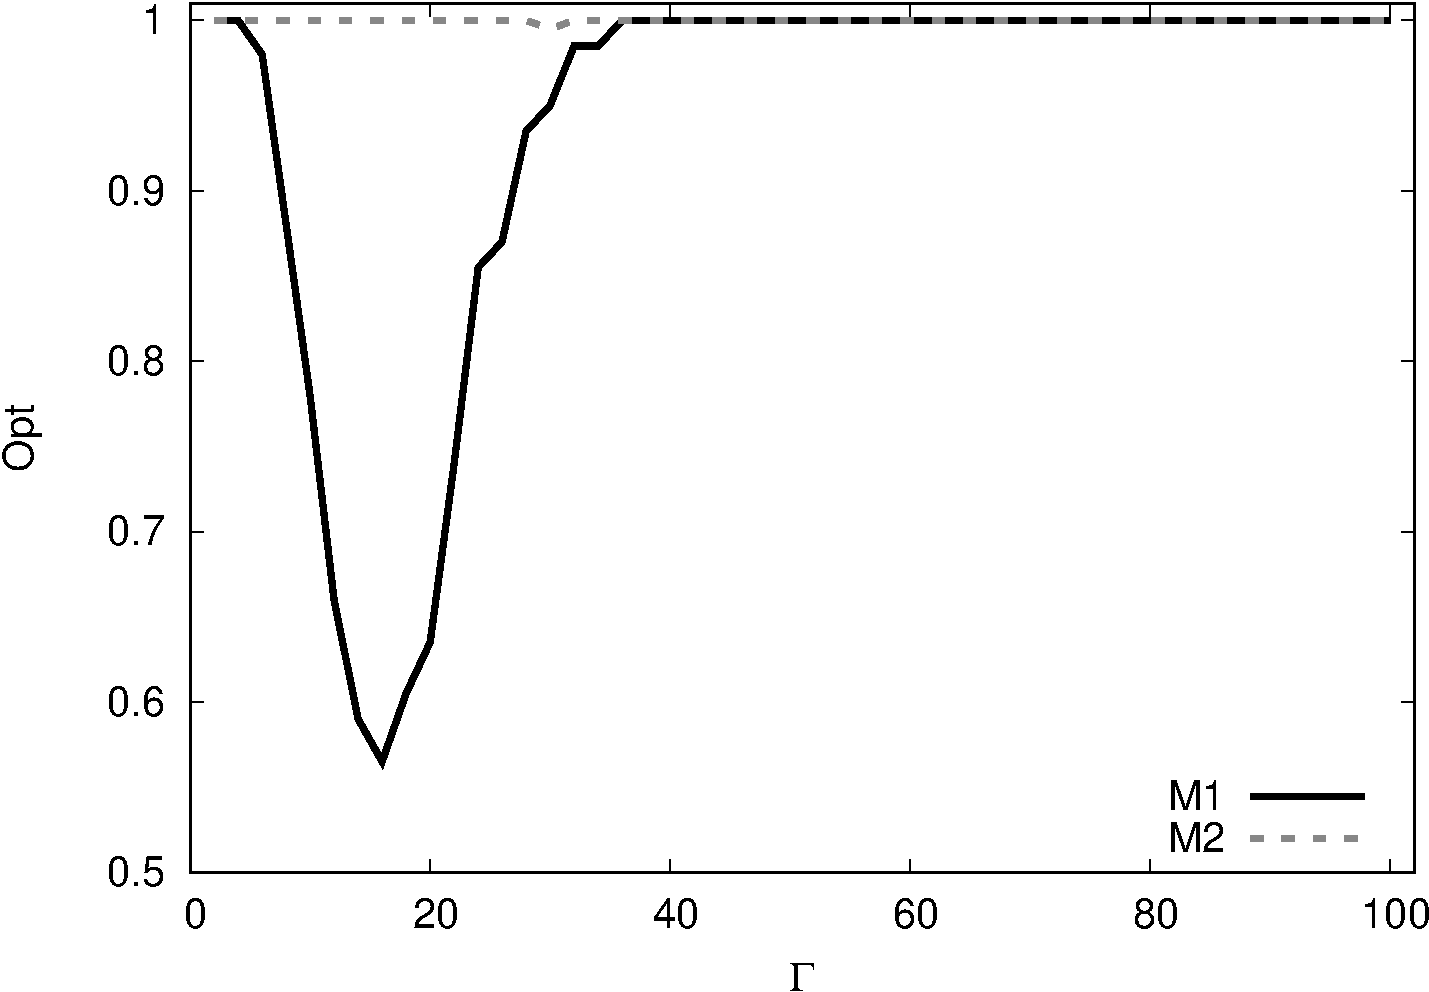
\includegraphics[width=0.48\textwidth]{img/plot-opt1.pdf}}%
\hfill
\subfigure[Instances $I_2$.\label{fig:opt2}]{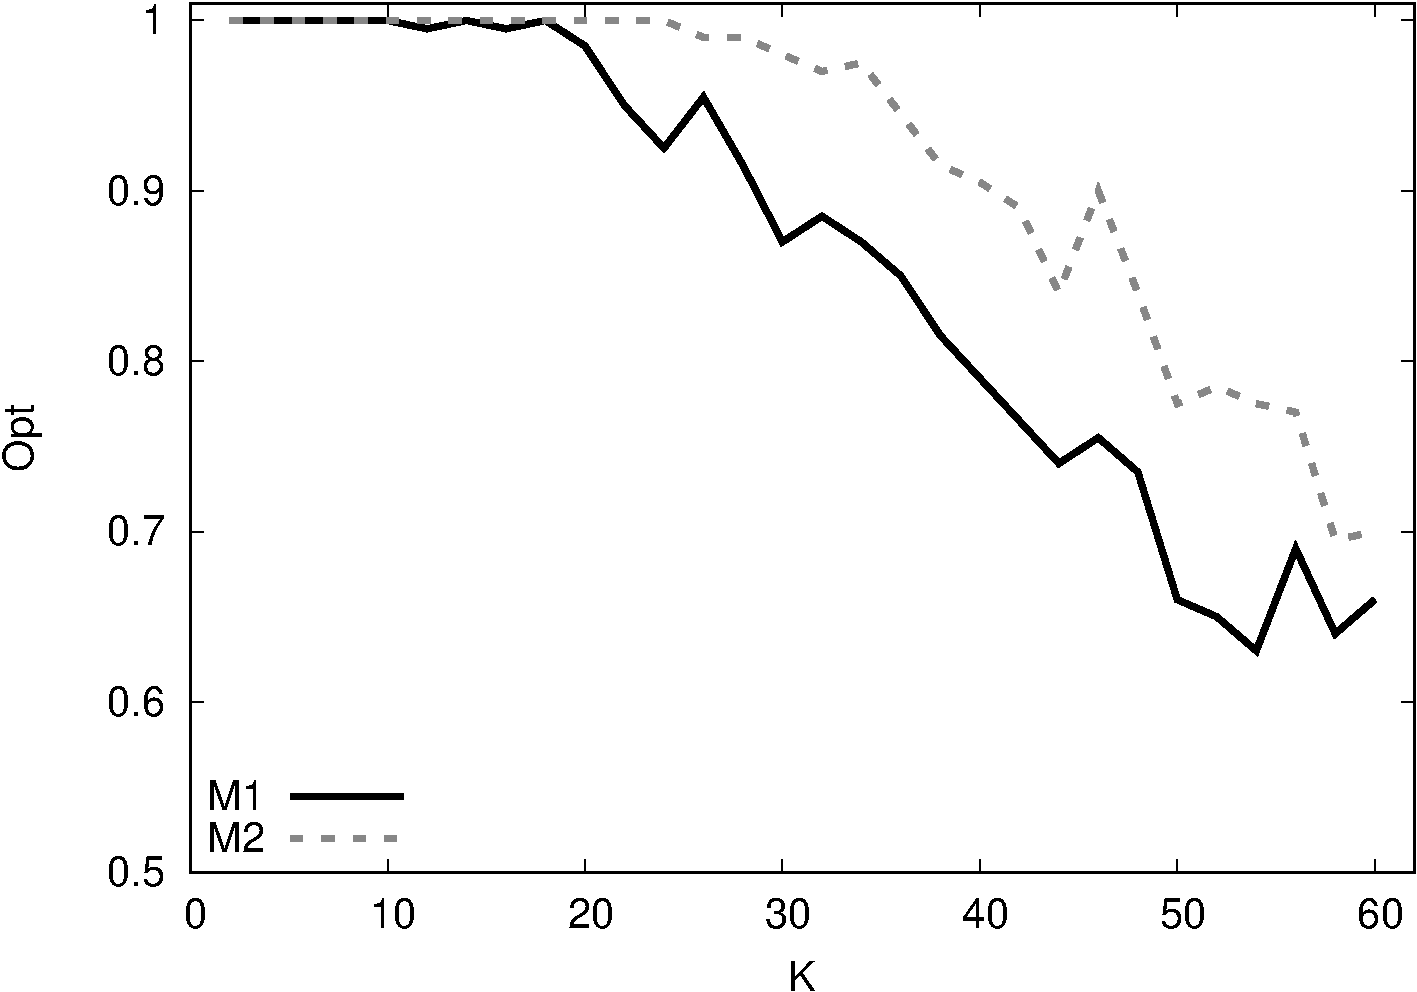
\includegraphics[width=0.48\textwidth]{img/plot-opt2.pdf}}
\end{center}
\caption{Ratio of instances solved to optimality for varying $\Gamma$ ($I_1$) and $K$ ($I_2$).\label{fig:opt}}
\end{figure}

This can be seen in more detail in Figure~\ref{fig:time1}, where we show the average computation time for M1 and M2. Any instance that could not be solved to optimality counts as 900 seconds towards this average.
The peak in computation times for M2 around $\Gamma=16$ is visible again; at the same time, we see that also approach M2 follows a similar curve as M1, while much less severe.

\begin{figure}[htb]
\begin{center}
\subfigure[Instances $I_1$.\label{fig:time1}]{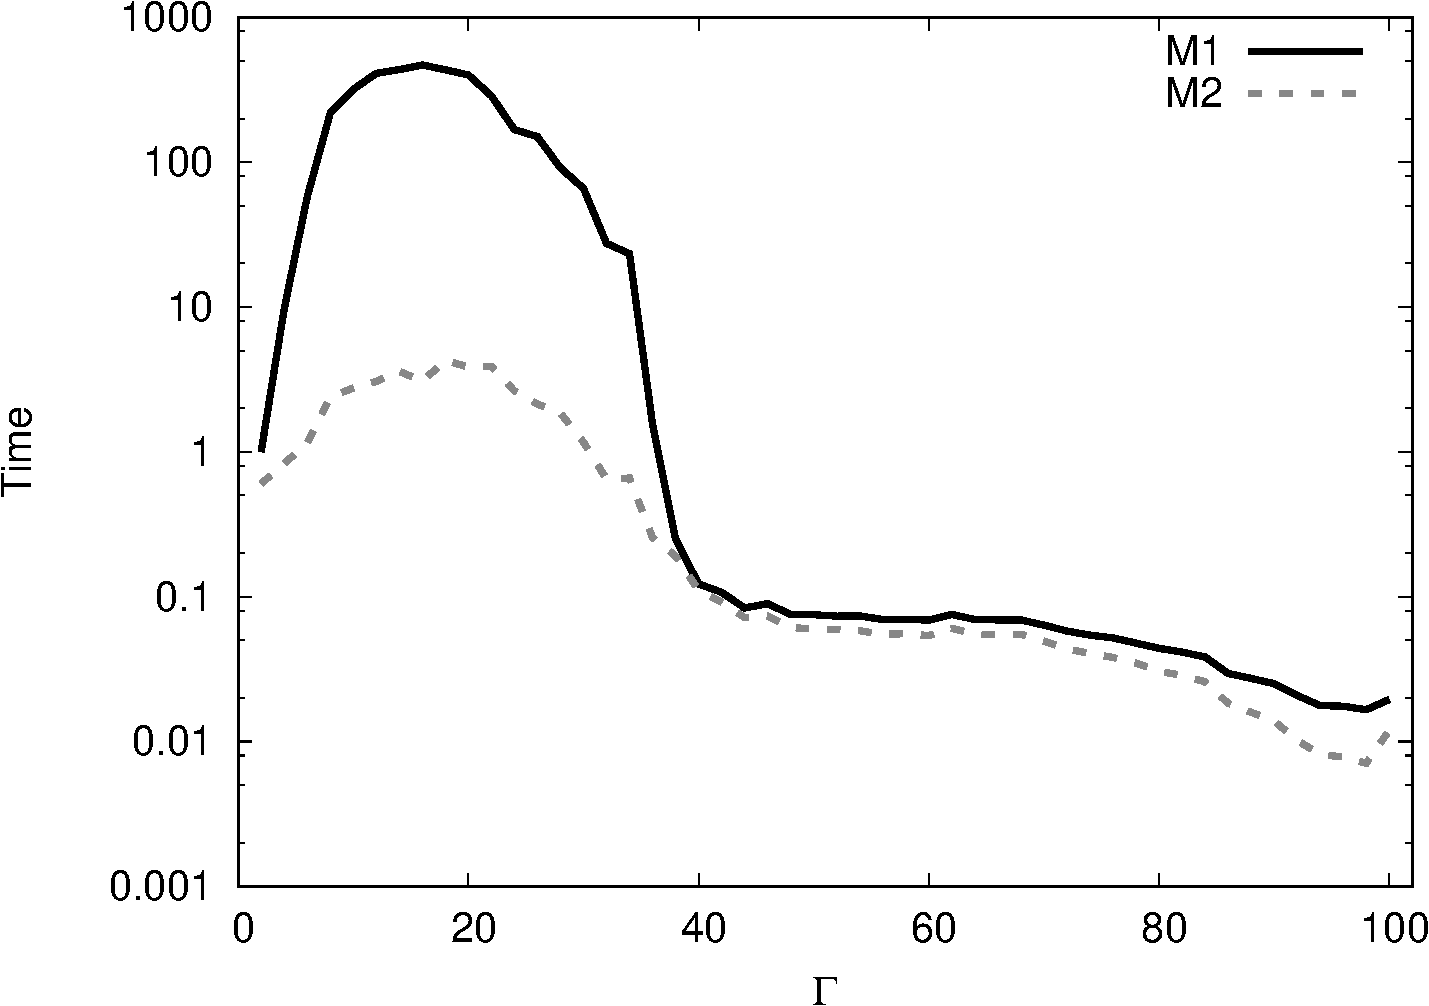
\includegraphics[width=0.48\textwidth]{img/plot-time1.pdf}}%
\hfill
\subfigure[Instances $I_2$.\label{fig:time2}]{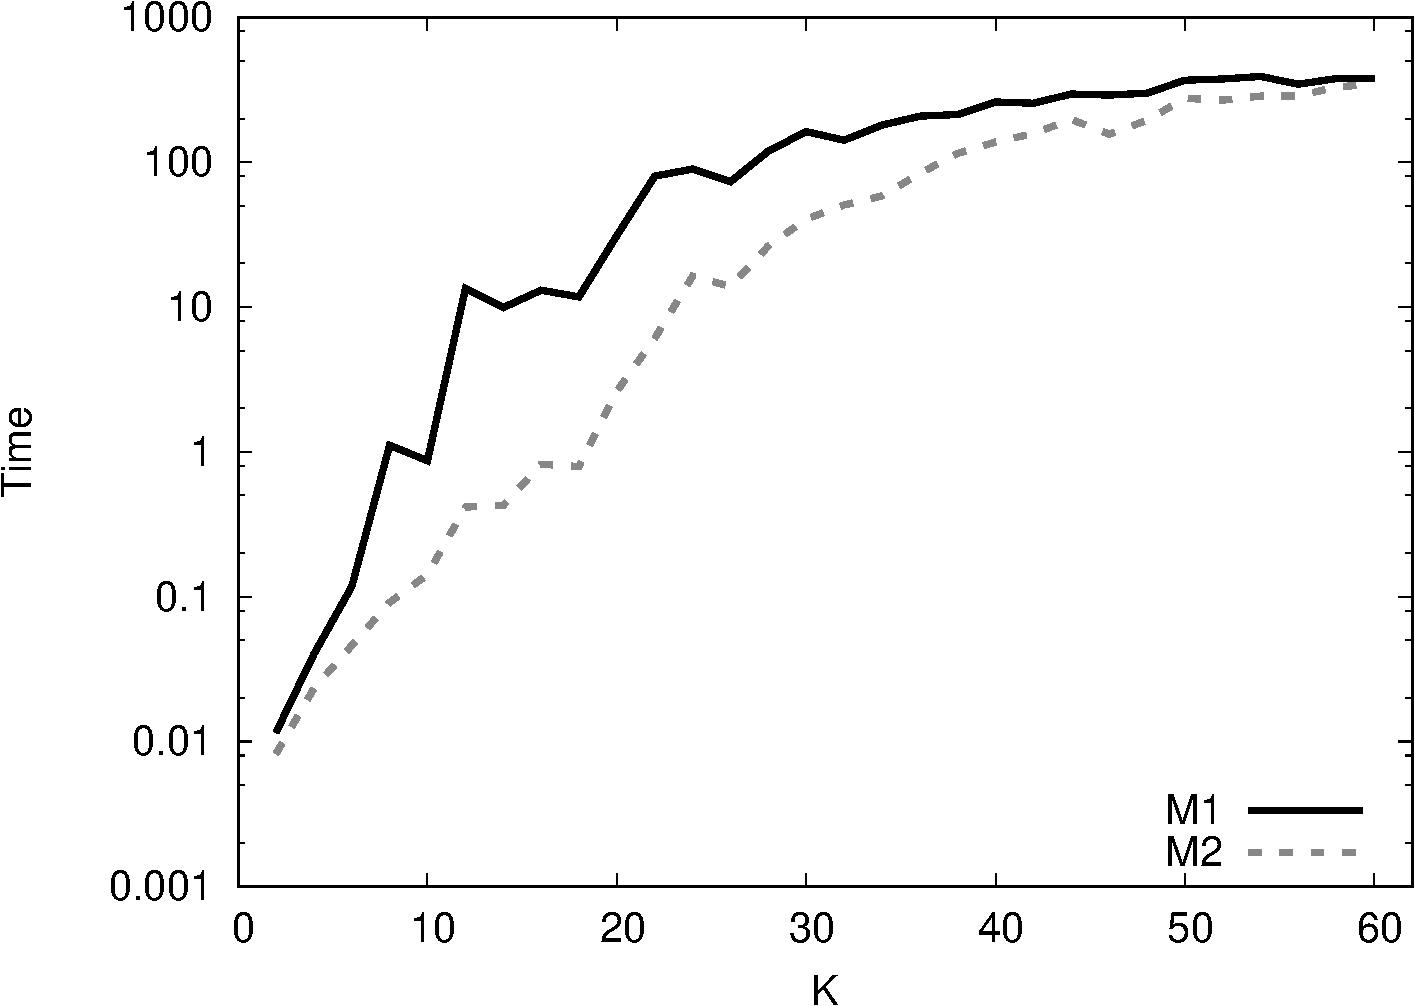
\includegraphics[width=0.48\textwidth]{img/plot-time2.pdf}}
\end{center}
\caption{Average truncated solution time in seconds for varying $\Gamma$ ($I_1$) and $K$ ($I_2$). Logarithmic vertical axis.\label{fig:time}}
\end{figure}	

A direct comparison between computation times for each instance is given in Figure~\ref{fig:tvst1}. Here, each point corresponds to one of the $10,000$ instances (note that both axes are logarithmic). A point below the diagonal indicates that M2 requires less time than M1 on this instance. For only few instances of $I_1$ it is faster to use M1 instead of M2, and none of these require more than one second to solve.

\begin{figure}[htbp]
\begin{center}
\subfigure[Instances $I_1$.\label{fig:tvst1}]{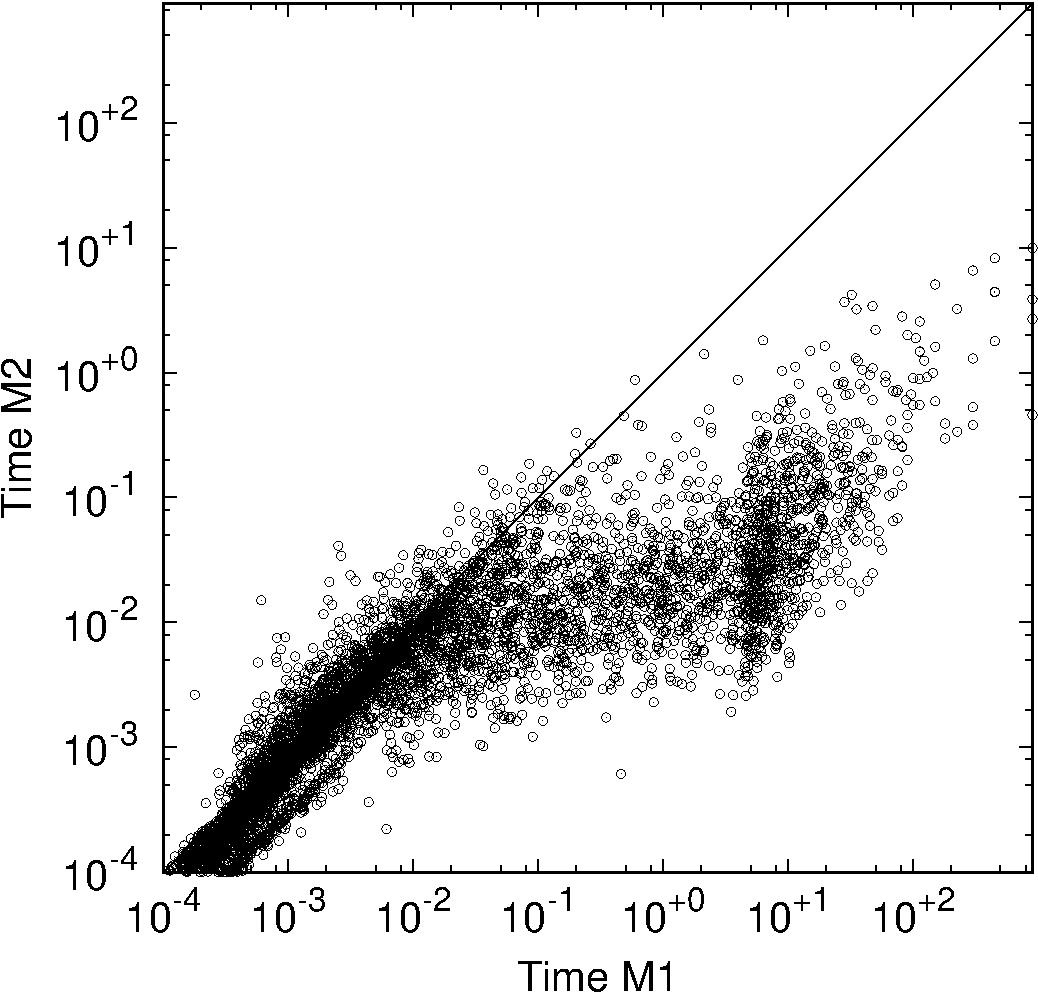
\includegraphics[width=0.48\textwidth]{img/plot-tvst1.pdf}}%
\hfill
\subfigure[Instances $I_2$.\label{fig:tvst2}]{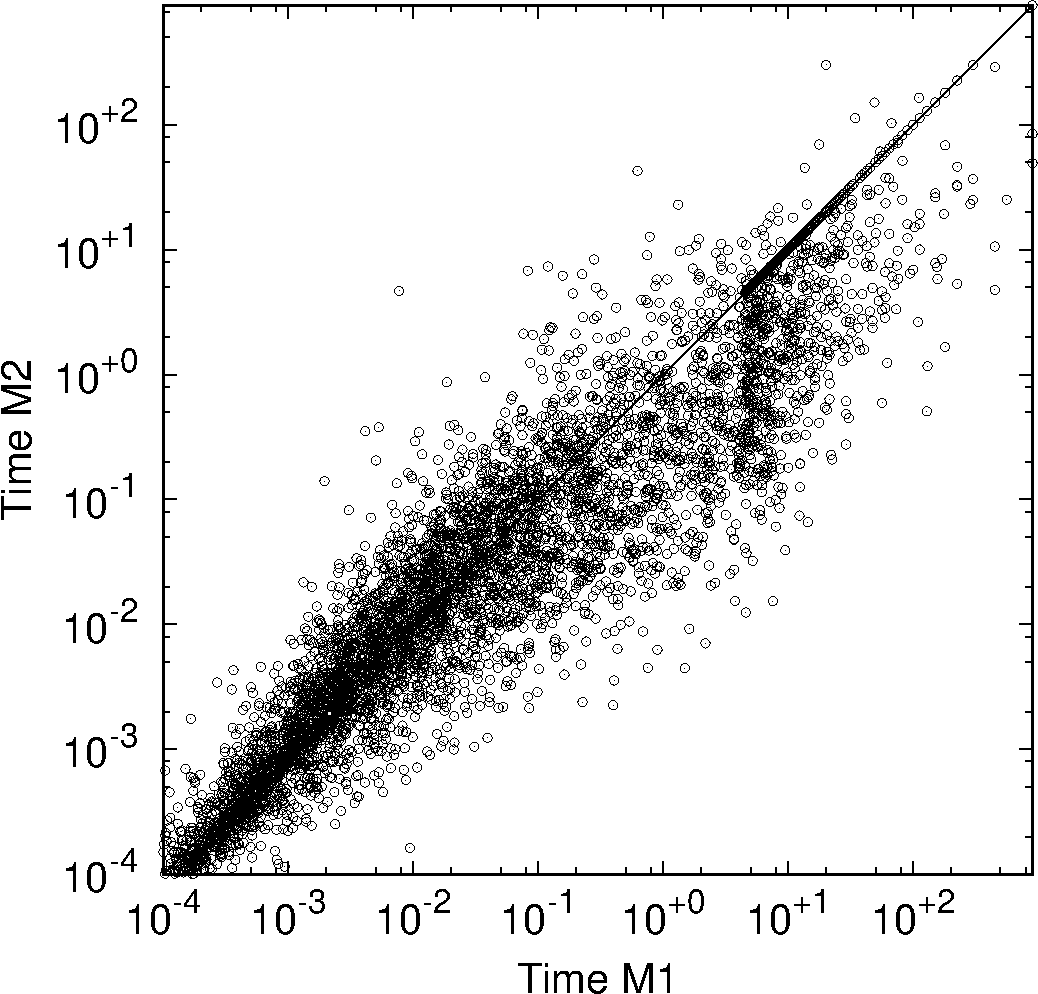
\includegraphics[width=0.48\textwidth]{img/plot-tvst2.pdf}}
\end{center}
\caption{Instance-by-instance comparison of solution times. Logarithmic axes.\label{fig:tvst}}
\end{figure}

Finally, we also present the average number of iterations required to prove optimality by each method in Figure~\ref{fig:it1}. In this average we only consider those instances that were solved to optimality by both methods. The minimum number of iterations is 2 (lower and upper bounds coincide after generating one scenario), and is achieved on all instances by both methods for $\Gamma \ge 54$. Instances with $\Gamma=16$ require an average of $18.25$ iterations to solve by M1, while this remains at $9.66$ for M2.

\begin{figure}[htbp]
\begin{center}
\subfigure[Instances $I_1$.\label{fig:it1}]{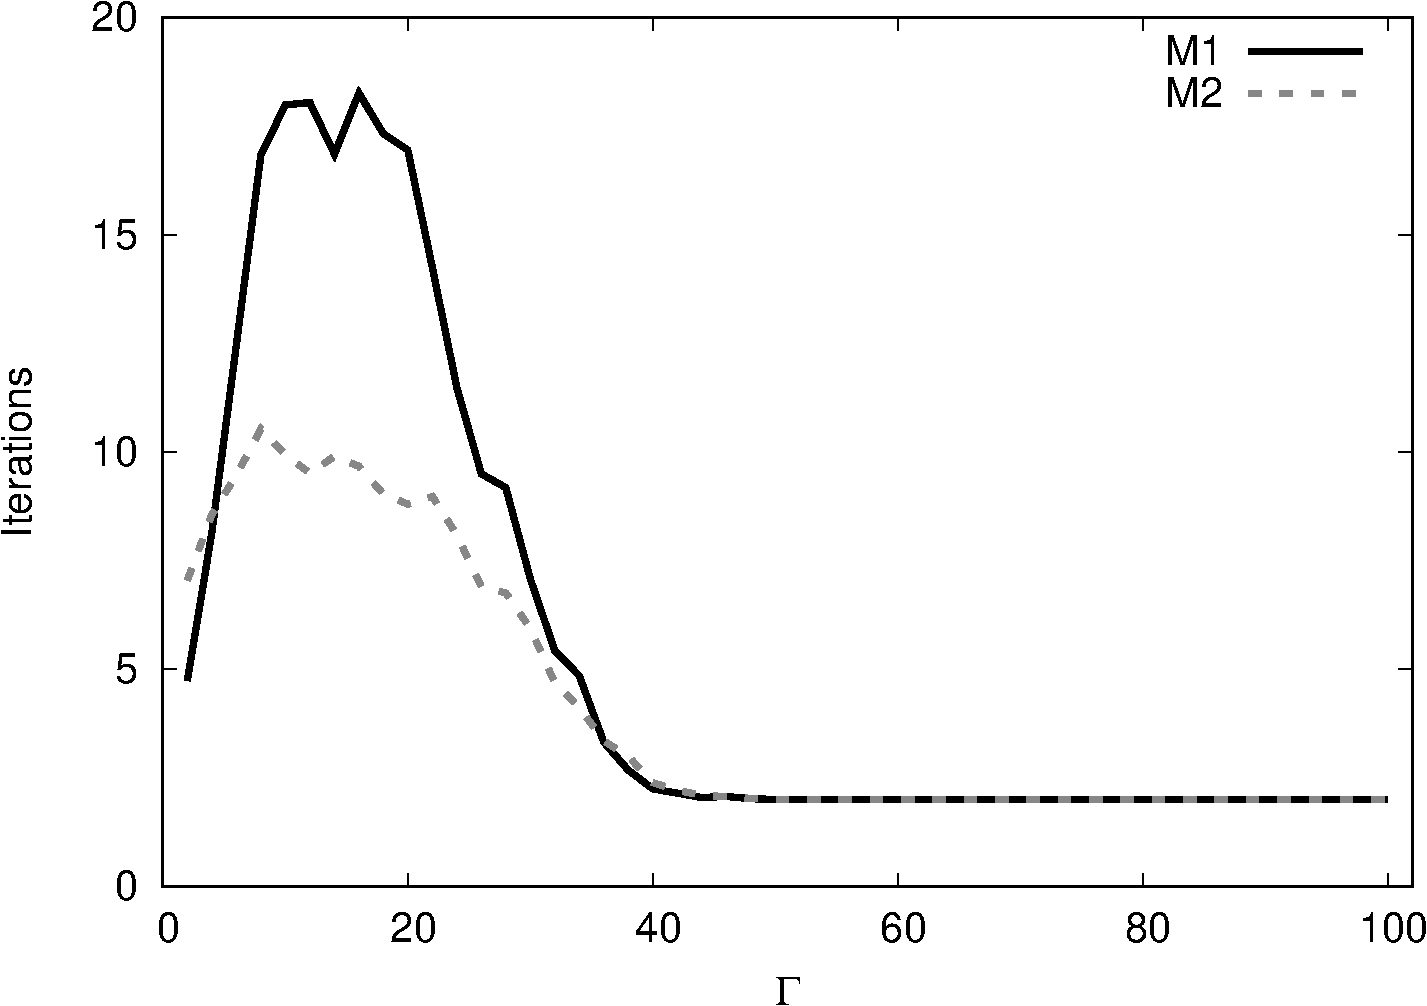
\includegraphics[width=0.48\textwidth]{img/plot-it1.pdf}}%
\hfill
\subfigure[Instances $I_2$.\label{fig:it2}]{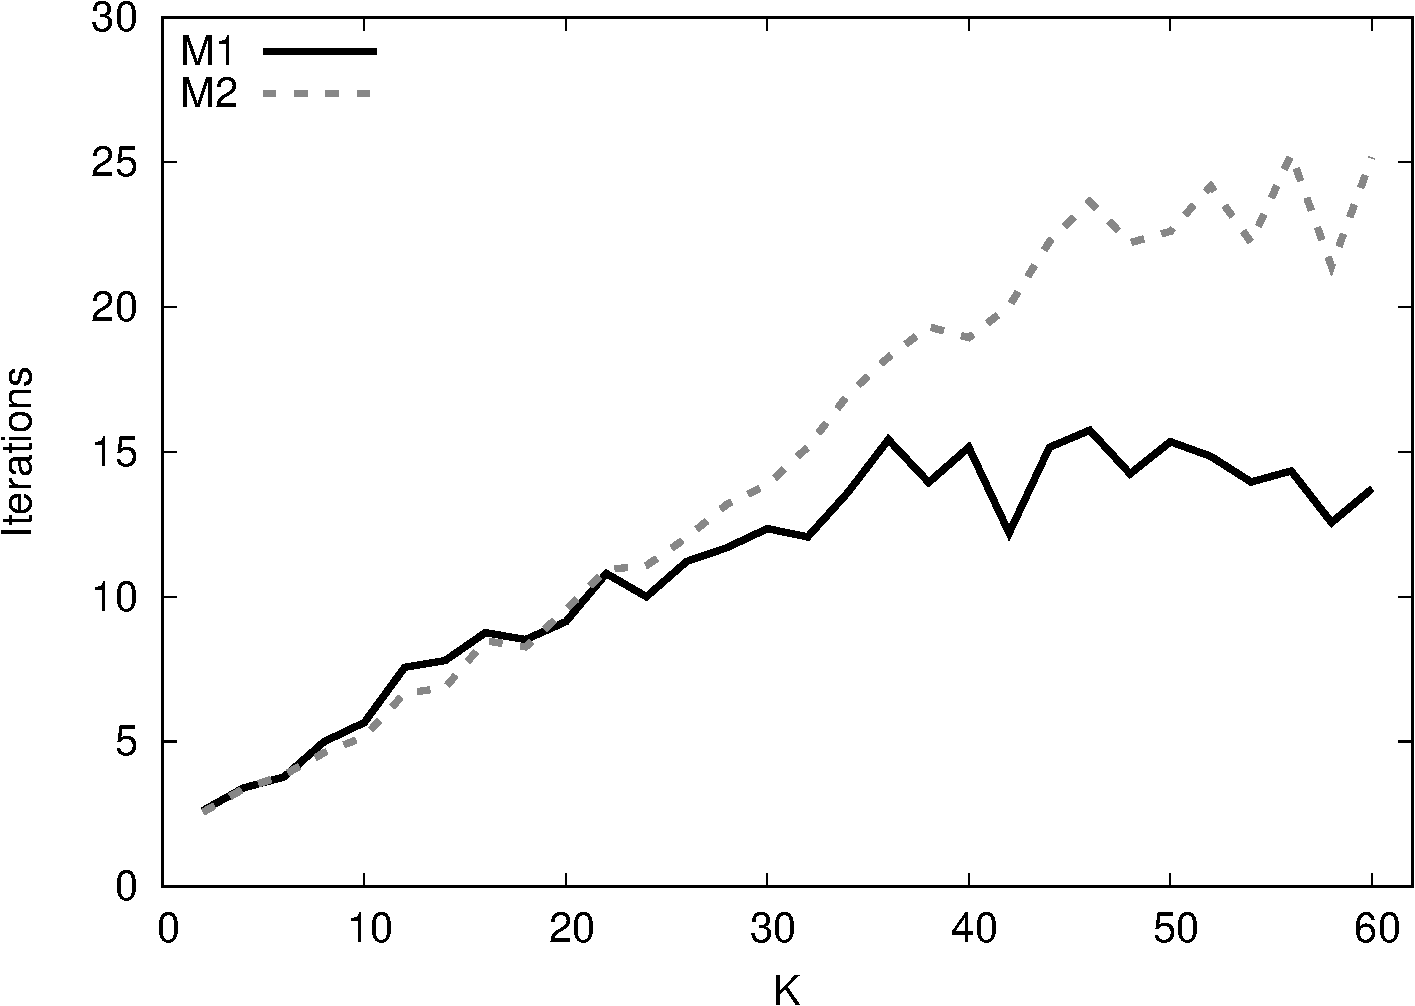
\includegraphics[width=0.48\textwidth]{img/plot-it2.pdf}}
\end{center}
\caption{Average number of iterations for varying $\Gamma$ ($I_1$) and $K$ ($I_2$).\label{fig:it}}
\end{figure}	

We now compare these findings with the results for instance set $I_2$. Note that with increasing value $K$, also the number of items $n$, and the parameters $\Gamma$ and $k$ increase. We therefore expect both M1 and M2 to perform worse for increasing $K$. Considering the number of instances solved to optimality as presented in Figure~\ref{fig:opt2}, this can be confirmed. The number of instances solved to optimality by M1 remains lower than those solved by M2. The average computation times as shown in Figure~\ref{fig:time2} also increase in $K$, where M2 is faster on average. A direct comparison of computation times for each instance as presented in Figure~\ref{fig:tvst2} shows that points are much more closely aligned to the diagonal than in Figure~\ref{fig:tvst1}. This indicates that M2 remains the better approach for most instances, but results tend to be more mixed. In one specific instance, M2 required 300 seconds, while M1 only required 20 seconds.

Considering the average number of iterations given in Figure~\ref{fig:it2}, we find another difference to instance set $I_1$. Up to around $K=20$, both approaches require a similar number of iterations. For larger values of $K$, this number keeps on increasing for M2, whereas this is not the case for M1. In comparison with Figure~\ref{fig:it1}, we see that the maximum average number of iterations for M1 is even smaller for $I_2$ than for $I_1$.

To summarize these findings, we note that M2 can solve all instances (but one) of size $10\times 10$ in a matter of a few seconds, and clearly outperforms M1 in these cases, particularly for parameters $\Gamma$ in the region of $[\sqrt{n},3\sqrt{n}]$. Due to the way scenarios are generated, the performance of M2 depends less on $\Gamma$ than the performance of M1. For instances of size $K \times 3$ with increasing $K$, this advantage of M2 is less pronounced. While M2 continues to show the better performance, results tend to be more mixed.

Overall, M2 performs better, which highlights the importance of the structural insights into the adversarial problem gained in Section~\ref{sec:adv}.

\section{Conclusion}
\label{sec:conclusions}

In this paper we considered the following robust variant of the representatives selection problem. Given $K$ sets of items called parts, we first choose $p_j$ items from each part $j\in[K]$. Then an adversary creates a cost scenario by increasing the costs of up to $\Gamma$ many items. We can now update our solution by exchanging up to $k$ items over all parts. The aim is to minimize the overall costs given by the costs of the first-stage solution, and the worst-case costs of the second-stage solution.

While this problem has been introduced nearly a decade ago, its complexity has remained open. This is perhaps not surprising, as an optimal solution can be quite counter-intuitive. An example provided in this paper demonstrates that it may be necessary to choose a dominated item in the first stage, i.e., an item that is worse with respect to every cost vector compared to another item from the same part.

We showed that it is possible to solve the adversarial problem in polynomial time and used this result to derive a compact mixed-integer programming formulation for the recoverable robust problem. We further prove that the recoverable robust problem is NP-hard, even if $n_j=2$ and $p_j=1$ for all parts $j\in[K]$. We also showed that the special case with $K=1$ is NP-hard, even if $k=1$. In the special case that $k=\Gamma=1$, this problem allows a polynomial time solution algorithm. This method is based on identifying two basic strategies that represent all possible attacks of the adversary. We can then construct a solution for each of these strategies, such that this strategy is in fact preferred by the adversary over the other. The better of these two solutions is optimal for the recoverable robust problem. Table~\ref{tab:summary} summarizes selected complexity results of this paper.

\begin{table}[htb]
\begin{center}
\begin{tabular}{rr|c|c|c}
 & & \multicolumn{3}{c}{$\Gamma$} \\
 & & 0 & 1 & general \\
 \hline
 & & & & \\[-1.5ex]
\multirow{8}{*}{$k$} & \multirow{2}{*}{0} & \multirow{2}{*}{P (Obs~\ref{obs1}/\ref{obs2})} & \multirow{2}{*}{P (Obs~\ref{obs1})} & \multirow{2}{*}{P (Obs~\ref{obs1})}\\
& & & & \\[-1.5ex]
 & & & & \phantom{for $p_j=1,n_j=2$} \\
\cline{3-5} & & & & \\[-1.5ex]
 & \multirow{2}{*}{1} & \multirow{2}{*}{P (Obs~\ref{obs2}))} & P  (Th~\ref{thm:easy_case_RRRS}) & NPC (Th~\ref{th3}) \\
 &   &   \phantom{for $p_j=1,n_j=2$}     & for $p_j=1,n_j=2$ & for $K=1$  \\
 & & & & \\[-1.5ex]
\cline{3-5} & & & & \\[-1.5ex]
 & \multirow{2}{*}{general} & \multirow{2}{*}{P (Obs~\ref{obs2}))} & \multirow{2}{*}{?} & NPC  (Th~\ref{th:hardness}) \\
 &         &         &   & for $p_j=1$
\end{tabular}
\end{center}
\caption{Selection of complexity results for RRRMSP with discrete budgeted uncertainty.\label{tab:summary}}
\end{table}


In computational experiments we compared two iterative methods that scale differently in the problem parameters. While the straight-forward scenario generation method is sensitive to the size of $\Gamma$, a second method that is based on structural insight into the adversarial problem can be expected to be more sensitive to the number of parts $K$.

Many interesting avenues for further research arise. 
While these results cover many complexity aspects of the problem, the complexity for constant $\Gamma$ remains open. Additionally, our reductions are based on weakly NP-hard problems, which means that it remains an open question if pseudopolynomial solution methods exist.
It seems likely that the proof of Theorem~\ref{thm:easy_case_RRRS} can be extended to general values $n_j$, if $p_j=\Gamma = k = 1$ holds. There still remain two basic adversarial strategies in this case; one where the chosen item of a part has its costs increased, and one where the cheapest item not chosen in a part has its cost increased. This may lead to an enumeration-based solution method along similar lines as presented in the proof.
Beyond the problem considered here, the complexity of other problem variants remains open as well. These include two-stage representatives selection (where an incomplete solution is built in the first stage) or other uncertainty sets, such as continuous budgeted uncertainty. In particular, it is an interesting question to determine the precise circumstances under which the algorithmic technique to derive a polynomial-time algorithm can also be extended to other problems.










\chapter{Assistance and Interdiction Problems on Interval Graphs}
\label{ch:interdiction}

\section{Introduction}

%\cite{bazgan2019more}

\emph{Network interdiction} \cite{NetworkInterdictProblemsBookChapter} is a vibrant and fast-growing area of research. 
A network interdiction problem is a min–max or max–min problem 
involving a graph parameter $\pi$ and two opposing players: 
The goal of the second player, the \emph{network owner}, is to optimize $\pi$, while the goal of the first player, the \emph{interdictor}, 
is to alter the network in such a way to maximally impair the owner's objective. 
Interdiction problems are fundamental problems in network 
analysis, because they tell us, which parts of a network are most susceptible 
to failure or attack \cite{criticalNodeDetectionSurvey}. 
One important type of network interdiction problems
is the \emph{most vital nodes problem} with respect to different graph parameters $\pi$. 
Here, we are given a graph, and some natural number $k$ called the \emph{budget}. The interdictor is allowed to delete up to $k$ vertices from the graph in order to impair $\pi$. For example, if the parameter $\pi = \alpha$ is the independence number, then the interdictor seeks to delete up to $k$ vertices from the graph, such that the size of the largest independent set in the remaining graph is minimized. The problem is to compute which vertices to select.

The most vital nodes problem has been considered for many different parameters, and many different special graph classes. (See e.g.\ \cite{baier2010length,complexityOfFindingMostVitalNodesShortestPath,mostVitalNodesWrtIndSet,mostVitalLinksNodes1982,mahdavi2014minimum}.) Diner et al. \cite{diner2018contractionDeletionBlockers} initiated the investigation of the most vital nodes problem on interval graphs. 
With respect to the clique number, they proved that a simple greedy-algorithm 
solves the most vital nodes problem on interval graphs. However, with respect to the independence number $\alpha$, they could not determine the complexity of the most vital nodes problem on interval graphs and left it as an open question~\cite[(Q2)]{diner2018contractionDeletionBlockers}.

In this paper, we positively answer (Q2): On interval graphs, the most vital nodes problem with respect to $\alpha$ can be solved in polynomial time.  Moreover, we extend this result to a much more general framework. For many graph parameters, the most vital nodes problem is a special case of the framework.

\subsection{The Shrink-Expand Framework} 
We propose a new framework, the \emph{shrink-expand framework}, for interdiction problems specifically 
for interval graphs. It revolves around \emph{shrinking} and \emph{expanding} intervals. Here, one is given two intervals $I$ and $I'$, such that either $I' \subseteq I$, or $I' \supseteq I$. The interval $I$ is called the \emph{original interval}, and the interval $I'$ is called the \emph{replacement interval} .
\begin{itemize}
\item If $I' \subseteq I$, then the operation of substituting the original interval $I$ with the smaller interval $I'$ is called \emph{shrinking the interval.}
\item  If $I' \supseteq I$, then the operation of substituting the original interval $I$ with the bigger interval $I'$ is called \emph{expanding the interval.}
\end{itemize}
 
We study interdiction problems with respect to shrinking and expanding intervals. As an input, we are given a fixed list $I_1,\dots,I_n$ of original intervals, and a fixed list $I'_1,\dots,I'_n$ of replacement intervals. For each $j=1,\dots,n$, the interval $I'_j$ is the replacement of the interval $I_j$, and we have $I'_j \subseteq I_j$ or $I'_j \supseteq I_j$.
Furthermore, we are given a budget $k \geq 0$. We start with the interval graph on the original intervals $I_1,\dots,I_n$.
In order to impair $\pi$, the interdictor can then choose a set of at most $k$ intervals and shrink (expand) the chosen intervals.
The question for the interdictor is now, which intervals to select in order to maximally impair $\pi$. For all the graph parameters considered in this paper, only one of shrinking or expanding makes sense. For example, in the clique number interdiction problem, the network owner seeks to find a clique of maximal size, and the interdictor impairs this objective by shrinking intervals. In the next section, we will list for each problem considered, whether one has shrinking or expanding intervals.

For many graph parameters, the shrink-expand framework contains the most vital nodes problem as a special case for the following reason: Consider a pair of original interval $I_j$ and its replacement interval $I'_j$, such that the replacement interval $I'_j = \emptyset$ is empty. The act of shrinking $I_j$ down to $I'_j$ corresponds to removing all edges from the corresponding vertex $v$ in the interval graph. For the graph parameters of  clique number and shortest path, it is easily seen that removing all incident edges from a vertex is equivalent to deleting it from the graph. Therefore, if every single replacement interval is empty, we have exactly the most vital nodes problem. For the graph parameter of independent set, an analogous observation holds. (Here, one chooses the replacement interval so large, that it intersects every other interval.)


While interdiction problems are min-max or max-min type of problems, the shrink-expand framework allows us to also consider \emph{assistance problems}, which are min-min or max-max type of problems. An assistance problem is a two-player problem, where the first player selects at most $k$ intervals to shrink (expand), and the second player optimizes some graph parameter $\pi$. But this time, the two players have a shared objective, instead of a conflicting one. For example, in the assistance problem for the clique number, one has expanding intervals, and the question is which intervals to expand in order to get an interval graph with maximum possible clique number.
If the interdiction problem has shrinking intervals, the assistance problem has expanding intervals, and vice versa. Assistance problems are interesting to consider, as they are the natural counterpart to interdiction problems. 

In this paper, we consider the interdiction and assistance problem for the following 
four classical graph parameters: 
Independence number $\alpha$, maximum clique size $\omega$, shortest path, 
and the scattering number (a graph parameter determining the Hamiltonicity property of interval graphs). 

\subsection{Related Work}
The area of interdiction problems on graphs has gained significant attention in 
the computer science literature (see eg.~\cite{NetworkInterdictProblemsBookChapter}).
The \emph{most vital nodes} problem for graph parameter $\pi$ is the problem where the interdictor is given a budget of $k$ vertex deletions and wants to maximally impair $\pi$. (In the earlier literature, the name only refers to the case $\pi =$  shortest path \cite{mostVitalLinksNodes1982}.)  In the very closely related \emph{vertex blocker} problem, the interdictor is given a threshold $t < \pi(G)$, and we wish to compute the required budget $k$ to reduce $\pi(G)$ down to $t$ \cite{shortPathsInterdictionTotalAndNodeWise}. In this paper, the difference is of no concern: We consider $k, t$ as part of the input, and in this case it is clear that if one problem is in $P$, so is the other. Many different parameters $\pi$ have been considered for both problems, see e.g.\ Nasirian et al. for a short summary \cite{nasirian2019exact}.
It is easy to see that the most vital nodes problem can be modeled as a special case of the interdiction problem in the shrink-expand framework.
Lewis and Yannakakis proved that for every hereditary and nontrivial graph parameter $\pi$, 
the most vital node problem is NP-complete in general graphs \cite{metaTheoremHereditary}.
 
%We give a solution to (Q2) in (ref) and also show in the appendix how to solve their question (Q1) with the same method.
The most vital nodes problem for parameters $\alpha$ and $\omega$ are well studied, 
even for special graph classes~\cite{mostVitalNodesWrtIndSet,costa2011minimum},
but interval graphs have not yet been investigated. Also, the most vital nodes 
problem for shortest paths has a long history~\cite{baier2010length,complexityOfFindingMostVitalNodesShortestPath,mostVitalLinksNodes1982,shortPathsInterdictionTotalAndNodeWise}.
When considering the most vital \emph{edges}, instead of the most vital nodes, there are results for interval graphs with respect to the parameter of shortest path. Bazgan et al.\ conjectured this problem to be polynomially solvable for unit interval graphs \cite{bazgan2019more} and Bentert et al.\ proved this conjecture \cite{bentert2019lengthboundedcuts}.


%For the replacement intervals, we allow the cases $a_i' = b_i'$ or $a_i'=-\infty$, 
%$b_i'=\infty$ and make the (slightly unusual) definition $[x,x] := \emptyset$. 
%Depending on $\pi$, this has the following consequence: 
%If interdiction is achieved by shrinking (for example if $\pi$ = max.\ clique size),
%then the case $a_i' = b_i'$ corresponds to the deletion of a vertex. 
%If interdiction is achieved by expanding (for example if $\pi$ = max.\ independent set size), 
%then the case $a_i' =-\infty, b_i=\infty$ corresponds to the deletion of a vertex. 
%Therefore, the shrink-expand framework includes the most vital nodes problem as a special case.

%Additionally, regarding a conjecture about the most vital edge problem by Bazgan et al.\ \cite{bazgan2019more}, our results show that this conjecture is true when one considers the most vital nodes instead of the most vital edges  (compare \cref{sec:related_work}).

\subsection{Our Contribution} 
We introduce a novel framework of graph modifications  
specific to interval graphs. The most vital nodes problem for interval graphs can be reduced to  this framework for all the graph parameters studied in this work. We observe that under this model not only interdiction but also the 
notion of an assistance problem can be defined. 
We study these two problem types for the four graph parameters $\alpha$, $\omega$, shortest path, and scattering number. The scattering number of an interval graph is related to its hamiltonian properties. In particular, we look at the \emph{interdiction problem with respect to Hamiltonicity}. Here, we are given an interval graph, which is hamiltonian, and the interdictor wishes to modify the graph such that it is not hamiltonian anymore.
We also obtain similar results for the related parameters of the path cover number, and graph toughness.

Even though the framework is general, we obtain polynomial-time algorithms
for 6 of the 8 studied problems. We obtain these results using (in some cases technically challenging) dynamic programs. 

\begin{theorem}
The following problems can be solved in polynomial time:
\begin{itemize}
\item The interdiction problem in the shrink-expand framework, for the parameters $\alpha$,  shortest path and Hamiltonicity.
\item The assistance problem in the shrink-expand framework, for the parameters $\omega$, $\alpha$, shortest path, and scattering number.
\item The most vital nodes problem on interval graphs, for the parameters $\alpha$, shortest path, and Hamiltonicity.
\end{itemize}
\end{theorem}

The interdiction problem in the shrink-expand framework for the parameter $\omega$ is shown to be NP-complete and $W[1]$-hard. \cref{tab:result-overview} provides an overview of our results. 
Our results for the independence number answer the question (Q2) stated by Diner et al. \cite[(Q2)]{diner2018contractionDeletionBlockers}. Additionally, in Appendix~\ref{app:contraction}, we show how to modify our proof to also answer their question (Q1), regarding edge contraction blockers on interval graphs~\cite[(Q1)]{diner2018contractionDeletionBlockers}.

\begin{table}
\centering
\setlength{\tabcolsep}{6pt}
\begin{tabular}{r|rrr}
$\pi$ & assistance & interdiction & most vital nodes\\
\hline
%connectedness & $\bigO(n)$ & $\bigO(n)$ \\
$\omega(G)$ & $\bigO(n)$ & \ NP-complete, W[1]-hard & $\bigO(n)$ \cite{diner2018contractionDeletionBlockers} \\
$\alpha(G)$ & $\bigO(kn)$ & $\bigO(kn^2)$ & $\bigO(k n^2)$\\
%min dominating set & $\bigO(kn^2)$ & ?\\
%ham-path & ? & $\bigO(kn^3)$ \\
Hamiltonicity & ? & $\bigO(kn^3)$ & $\bigO(k n^3)$\\
%ham-cycle & ? & ? \\
shortest path & $O(kn)$ & $O(n^4)$ & $\bigO(n^4)$
\end{tabular}
\caption{Overview of the results}
\label{tab:result-overview}
\end{table}



%[[Last, but not least, we remark that a second motivation for the shrink-expand framework is given by the area of \emph{fixed interval scheduling}. Kovalyov, Ng and Cheng write in their survey \cite{fixedIntervalSchedulingSurvey}, that \enquote{the defining characteristic of fixed interval scheduling problems is that each job has a finite number of fixed processing
%intervals. A job can be processed only in one of its intervals on one of the available machines, or is not processed at all.}
%%A decision has to be made about a subset of the jobs to be processed and their assignment to the processing intervals such that the intervals on the same machine do not intersect.
%
%Furthermore, they write that \enquote{these problems arise naturally in different real-life operations planning
%situations, including the assignment of transports to loading/unloading terminals, work planning for personnel, computer
%wiring, bandwidth allocation of communication channels, printed circuit board manufacturing, gene identification
%and examining computer memory structures.} 
%
%Specifically, many authors considered the \emph{Job Interval Selection Problem
%with $k$ intervals per job} (JISP$k$) \cite{nakajima1982complexity,spieksma1999approximability,chuzhoy2006approximation,erlebach2003interval}. Here, each job has exactly $k$ intervals attached to it, and the goal is to schedule as many jobs as possible on a single machine. Equivalently, we have to find an independent set of maximum size in an interval graph, which uses at most one interval in each predescribed $k$-tuple of intervals. It is known that already JISP2 is NP-complete and has no PTAS \cite{spieksma1999approximability}. The difference from JISP2 to the shrink-expand framework is, that in the shrink-expand framework we require for each job, that the two intervals attached to it are nested. We further require that at most $k$ of the \enquote{small} intervals may be selected (otherwise the problem becomes trivial). Our results show that in this case, JISP2 and other related scheduling problems are computable in polynomial time.]]\comment{paragraph [[...]] can be cut from the paper maybe}

\section{Preliminaries}
\label{sec:prelim}
Let $[n] = \fromto{1}{n}$ denote the set of the first $n$ positive natural numbers and $\mathbb{N}_0 = \mathbb{N} \cup \{ 0 \}$ denote the set of nonnegative integers. We use standard notation and terminology from graph theory to denote 
the common graph parameters studied in this work. 
Given a graph $G = (V,E)$ a  subset $S$ of $V$ is called a \emph{clique} if 
for each pair of distinct vertices $u,v \in S$, it holds that $\{u,v\} \in E$.
Analogously, a subset $S$ of $V$ is called an \emph{independent set} if for each pair 
of distinct vertices $u,v \in S$, it holds that $\{u,v\} \notin E$.  We denote by $\omega(G)$ the size of a maximum 
clique in $G$ and by $\alpha(G)$ the size of a maximum independent set in $G$.
A sequence $P = (v_0, v_1, \dots, v_{\ell})$ of pairwise distinct vertices of $G$ is called a \emph{path} in $G$ 
if each consecutive pair of vertices is connected by an edge.
We say $P$ starts in $v_0$ and ends in $v_{\ell}$. The number $\ell$ is called the length of the path. Given two vertices $s$ and $t$, 
the shortest path from $s$ to $t$ is a path starting in $s$, ending in $t$, and
of minimum length.
A sequence $C = (v_0, v_1, \dots, v_{\ell})$ of pairwise distinct vertices of $G$
is called a \emph{cycle} if, in addition to each consecutive pair of vertices being connected by an edge, 
also $\{v_{\ell}, v_0\} \in E$. A \emph{Hamilton path} in $G$ is a path consisting of all vertices of $G$
and a \emph{Hamilton cycle} in $G$ is a cycle consisting of all vertices of $G$. We 
call a graph $G$ \emph{hamiltonian} if there exists a Hamilton cycle in $G$.
A \emph{path cover} of $G$ is a set of vertex-disjoint paths $P_1, \dots, P_k$ 
such that each vertex of $G$ is contained in at least one path. The number $k$ of 
such paths is called the size of the path cover. Note that a path cover of size $1$ 
is a Hamilton path. If $S \subseteq V$ is a set of vertices, we denote by $G-S$ the graph obtained from $G$
by deleting the vertices in $S$ (and their incident edges) from $G$.

For $a < b$, the \emph{closed interval} $[a, b]$ is defined as $\set{x \in \R \mid a \leq x \leq b}$. It has \emph{startpoint} $a$ and \emph{endpoint} $b$. We furthermore define $[a, a] := \emptyset$. Note that this is non-standard, but it will turn out convenient to use. We only consider closed intervals in this paper. If $\mathcal{J} =  (J_1, \dots, J_n)$ is a sequence of intervals (possibly containing duplicates), then we denote by $\graph(\mathcal{J}) = (V,E)$ the corresponding \emph{interval graph}
where $V = [n]$ and for any $u,v \in V$, it holds that $\{u,v\} \in E$ if and only if 
$J_u \cap J_v \neq \emptyset$. Note that in the whole work, we identify the set of 
vertices of the graph with the integers from $1$ to $n$. Given a subset of vertices $X \subseteq [n]$, we denote by 
$\J[X] = \{ J_i \colon i \in X \}$ the set of corresponding intervals.
The sequence $\mathcal{J}$ is called an \emph{interval representation} of the graph $\graph(\mathcal{J})$. It is folklore that if $\mathcal{J}$ contains two intervals which have a common start- or endpoint, one can easily obtain a representation $\mathcal{J}'$ such that no two intervals have a common start- or endpoint and $\graph(\mathcal{J}') = \graph(\mathcal{J})$. We will therefore assume this property whenever it is convenient.



\begin{table}
\centering
\begin{tabular}{r|rr}
$\pi$ & assistance & interdiction\\
\hline
$\omega(G)$ & expand & shrink\\
$\alpha(G)$ & shrink & expand \\
Hamiltonicity & expand & shrink \\
shortest path & expand & shrink \\
scattering number & shrink & expand
\end{tabular}
\caption{Problems in the shrink-expand framework have either shrinking or expanding intervals.}
\label{tab:shrink-expand-overview}
\end{table}
A problem in the shrink-expand framework is defined by an input $(\I, \I', n, k)$. Here, $n$ is the number of vertices, $k \geq 0$ is the budget, $\I = (I_1, \dots, I_n)$ is the sequence of original intervals, and $\I' = (I'_1, \dots, I'_n)$ is the sequence of replacement intervals. The interval $I'_j$ is the replacement interval of the original interval $I_j$ for $j \in [n]$.  We have either $I'_j \subseteq I_j$ for all $j$ (\emph{shrinking} case), or $I'_j \supseteq I_j$ for all $j$ (\emph{expanding} case). \cref{tab:shrink-expand-overview} explains for all problems in the shrink-expand framework, whether we are in the shrinking case or the expanding case. Throughout the paper, we always use the letters $a$ and $b$ for start- and endpoints of $I_j$ and $I'_j$, that is $I_j = [a_j, b_j]$, and $I'_j = [a'_j, b'_j]$.

For a set $X \subseteq [n]$ of indices, we denote by $\I_X$ the sequence of intervals that is obtained from \las{the sequence} $\I$ after shrinking (expanding) the intervals with indices in $X$. Formally, 
\[(\I_X)_j = \begin{cases} I'_j & \text{if }j \in X \\
I_j & \text{if } j \not\in X. \end{cases}\]
When it is convenient, we can assume that each of $\I, \I', \I_X$ contains no duplicates and treat them as sets instead of sequences. We define $G_X := \graph(\I_X)$. We are interested in problems of the form 
\[ \max_{X \subseteq [n], |X| \leq k} \pi(G_X) \ \text{ or } \min_{X \subseteq [n], |X| \leq k} \pi(G_X)\]
where $\pi$ is some graph parameter. The problem is an \emph{interdiction problem} if it is a problem of max-min or min-max type. The problem is an \emph{assistance problem} if it is a problem of min-min or max-max type.

\section{Shortest Path}

In the shortest path interdiction problem, we are given a graph, and two specified vertices $v_s, v_t$. The interdictor wishes to maximize the length of a shortest path connecting $v_s$ and $v_t$. For interval graphs, we consider the following equivalent problem formulation: 
Given a set $Z$ of intervals and two numbers $s, t \in \R$, define $\dist_Z(s, t)$ to be the minimum number of intervals from $Z$, which one needs to \enquote{walk} from $s$ to $t$. (Here, by a walk, we mean a sequence $(X_1, \dots, X_d)$ of intervals, such that $s \in X_1$, $t \in X_d$, and $X_i$ intersects $X_{i+1}$ for $i \in \fromto{1}{d-1}$. For example, in \cref{fig:shortest_path_ex1}, we have $\dist_Z(0, y) = 3$ with the corresponding walk $(I_1,I_3,I_4)$.) 
For the interdiction problem, 
the input consists of the set $\I = \{ [a_1,b_1], \dots, [a_n, b_n] \}$ of original intervals, the set 
$\I' = \{ \las{[a'_1,b'_1]}, \dots, [a'_n, b'_n] \}$ of replacement intervals, two numbers $s, t \in \R$, and a budget $k \in \N_0$. We are in the shrinking case and want to determine 
\[\max\set{\dist_{\I_X}(s, t) : X \subseteq [n], |X| \leq k}.\] This problem variant is clearly equivalent to the problem described above. Furthermore, without loss of generality, we can assume that $s = 0 < t$, and that for all intervals $F \in \I \cup \I'$ one has $F \subseteq [0, t]$. (This is because it is never beneficial to walk to the left of $s$ or to right of $t$, so if some $F \in \I \cup \I'$ is not contained in $[s, t]$, we can replace $F$ by $F \cap [s, t]$ and still obtain an equivalent problem instance.) 

In the assistance problem, we are analogously given expanding intervals $\I, \I'$ and want to minimize the distance between $s$ and $t$ by expanding at most $k$ intervals. We show in this section that both problems can be solved in polynomial time.

\subsection{Assistance Problem}
As explained above, we are given expanding intervals $\I, \I'$ and want to determine 
\[ \min \{ \dist_{\I_X}(s, t) \colon X \subseteq [n], |X| \leq k \}. \]
There is a nice analogy for this problem: Suppose we are located on the real number line at point $s$ and want to get to point $t$. Furthermore, an interval $[a_i, b_i] \in \I$ is a road from $a_i$ to $b_i$ which we can use for this cause without paying a fee. Likewise, an interval $[a_i', b_i'] \in \I'$ is a road from $a'_i$ to $b_i'$, but it costs us a fee of one dollar to use. The assistance problem asks for the lowest amount of roads needed to travel from $s$ to $t$ while paying at most $k$ dollars. This can be solved using dynamic programming. 
\begin{theorem}

The assistance problem of shortest path in the shrink-expand framework can be solved in polynomial time. The algorithm can be implemented in $\bigO(kn)$ time, if we are given the list of all intervals sorted both with respect to startpoints and endpoints.
\end{theorem}


\begin{proof}
Consider the set $\mathcal{P} := \bigcup_{i=1}^n \set{a_i, b_i, a'_i, b'_i}$ consisting of all the start- and endpoints of intervals $F \in \I \cup \I'$. For each point $p \in \mathcal{P}$, let $\alpha(p)$ be the rightmost point one can reach from $p$ by using a single interval from $\I$. Formally, $\alpha(p) := \max\set{x \in \mathcal{P} \mid \las{x \neq p \text{ and }} \exists I \in \I: p, x \in I}$ or $\alpha(p) = -\infty$ if the set is empty. Likewise, let $\alpha'(p)$ be the rightmost point one can reach from $p$ by using a single interval from $\I'$, i.e.\ $\alpha'(p) := \max\set{x \in \mathcal{P} \mid \las{x \neq p \text{ and }} \exists I' \in \I': p, x \in I'}$ or $\alpha'(p) = -\infty$ if the set is empty. We claim that the set of all values $\alpha(p), \alpha'(p)$ for $p \in \mathcal{P}$ can be precomputed in linear time using a sweep line algorithm, provided that we already have the intervals sorted with respect to both the start- and endpoints. 

Indeed, \las{let $\mathcal{Q} := \bigcup_{i=1}^n \set{a_i,b_i}$.} Consider a sweep line starting at $-\infty$ going to $\infty$ \las{and stopping at every point in $\mathcal{Q}$ in increasing order. The algorithm has a variable $x$ which is initially $-\infty$. Whenever we encounter some point $a_i$, we update $x \gets \max\set{x, b_i}$. Whenever we encounter some point $b_j$, if currently $x = b_j$, then we update $x \gets -\infty$. It is easily proven by induction, that the variable $x$ always contains the correct value of $\alpha(p)$. The values $\alpha'(p)$ are computed analogously, only substituting $a_i, b_j$ by $a'_i, b'_j$ and $\mathcal{Q}$ by $\mathcal{Q}' := \bigcup_{i=1}^n \set{a'_i,b'_i}$. We have therefore shown how to compute all values of $\alpha(p), \alpha'(p)$ in $\bigO(n)$ time.}
 %(Note that we require a sorting of the intervals with respect to the startpoints, as well as with respect to the endpoints, as we need to iterate over $p \in \mathcal{P}$.)

Finally, consider the digraph $G$ on vertex set $\mathcal{P} \cup \set{-\infty}$ and the following arc set: For every $p \in \mathcal{P}$, it has one arc $e = (p, \alpha(p))$ and one arc $e' = (p, \alpha'(p))$. We call $e'$ an \emph{expensive} arc. Observe that $G$ is acyclic and has $\bigO(n)$ arcs. Furthermore, the solution to the assistance problem is given by the shortest path in $G$ from $s$ to $t$, which uses at most $k$ expensive arcs. But such a path can be computed using dynamic programming in $\bigO(kn)$ time, via the recursion formula
\begin{align*}
f(p, k') = \min\set{\min\set{f(p',k')+1 \mid (p',p) \text{ not expensive}},\\ \min\set{f(p',k'-1)+1 \mid (p',p) \text{ expensive}}} 
\end{align*}
with starting conditions $f(s, k') = 0$ for all $k' \in \fromto{1}{k}$ and $f(p, -1) = \infty$ for all $p \in \mathcal{P}$.
It is easy to show via induction that $f(p,k')$ is the length of the shortest path from $s$ to $p$
using at most $k'$ expensive arcs. At the end $f(t,k)$ is the optimal objective value for the given assistance problem.
\qed\end{proof}

\subsection{Interdiction Problem}
In this section, we prove: 

\begin{theorem}
\label{thm:shortest_path_interdiction}
The interdiction problem for shortest path in the shrink-expand framework can be solved in time $\bigO(n^4)$.
\end{theorem}

In order to enhance the readability of the proof, we employ the following strategy: First, we show that it suffices to solve the most vital nodes problem instead. Then we prove that the most vital nodes problem can be solved in polynomial time. Finally, we give an argument how the runtime can be improved.

\begin{lemma}
\label{lemma:shortest_path_reduction}
The interdiction problem for shortest path in the shrink-expand framework can be reduced to the most vital nodes problem for shortest path \las{on interval graphs}.
\end{lemma}
\begin{proof} 
Let $(\I, \I', k, s,t)$ be an instance of the interdiction problem, where $\I = \fromto{[a_1, b_1]}{[a_n, b_n]}$, $\I' = \fromto{[a'_1, b'_1]}{[a'_n, b'_n]}$, and $[a'_j, b'_j] \supseteq [a_j, b_j]$ for all $j \in \fromto{1}{n}$. Furthermore, $k \in \N_0$ is the budget, and $s, t \in \R$. We construct an equivalent instance of the most vital nodes problem. This instance is described by $(M, k, s, t)$, where $k, s, t$ stay the same as before, and $M$ is the following multi-set of intervals: $M$ contains one copy of $\I$ and $k+1$ copies of $\I'$, i.e.\ it has cardinality $n(k+2)$. More formally, for each $i \in \fromto{1}{n}$, let $N(i, k)$ be the multi-set, consisting of $k+1$ copies of $[a_i', b_i']$. The multi-set $M$ is then given by
\[M = \I \cup \bigcup_{i=1}^n N(i, k). \]
%that is, $M$ contains $n(k+2)$ elements.

We now claim that the interdiction problem for $\I, \I'$ has the same solution as the most vital nodes problem for $M$. In other words, we have the equality
\[\las{\max}_{X \subseteq [n], |X| \leq k} \dist_{\I_X}(s, t) = \las{\max}_{Y \subseteq M, |Y| \leq k} \dist_{M \setminus Y}(s, t). \]
In fact, to see \enquote{$\geq$}, whenever we have on the left-hand side a set $X \subseteq [n]$ describing the indices of intervals which are \las{shrunk} by the interdictor, 
we can also delete the same intervals in $M$ to get an equivalent term on the right-hand side. 
To see \enquote{$\leq$}, assume we have a multi-set $Y \subseteq M$ on the right-hand side. 
Observe that there is no $i \in \fromto{1}{n}$ such that $N(i, k) \subseteq Y$, simply because $|N(i, k)| = k+1$, 
but $|Y| \leq k$. But %if $|N(i, k) \cap X| \leq |N(i, k)|$, 
then the deletion of $N(i, k) \cap Y$ has no effect on the distance between $s$ and $t$. 
We can therefore assume that $Y \cap N(i,k) = \emptyset$ for all $i$, which implies $Y \subseteq \I$. 
Hence, the interdictor can also shrink the same intervals in $\I$ to get an equivalent term on the left-hand side. This completes the proof.
\qed\end{proof}

Certainly, the reduction described by the previous proof will increase the size of the instance by a factor of roughly $k$. We show at the end of this section how to overcome this problem.

\begin{figure}
\centering

\includegraphics[scale=1,page=2]{chapter-3-interdiction/figure_shortest_path}
\caption{\las{Let $Z := \fromto{I_1}{I_6}$. We have $\dist_Z(0,y)= 3$. The point $x$ is 2-critical with respect to $Z$. We have $\rel(x) = \fromto{I_1}{I_4}$ and $\betw(x,y) = \set{I_5}$.}}
\label{fig:shortest_path_ex1}
\end{figure}
%------------------------------
%-----------------------------
\begin{figure}
\centering

\includegraphics[scale=1,page=3]{chapter-3-interdiction/figure_shortest_path}
\caption{\las{The set $\set{I_2, I_3}$ is in state $(v,x,2)$, but not in state $(v,w,2)$, since the interval $I_3$ goes beyond $w$.}}
\label{fig:shortest_path_ex2}
\end{figure}
%------------------------------
%-----------------------------
\begin{figure}
\centering

\includegraphics[scale=1,page=4]{chapter-3-interdiction/figure_shortest_path}
\caption{\las{If $Z := \set{I_1, I_3, I_4}$, then $Z \subseteq \rel(x)$ is in state $(x,y,3)$. The set $Z$ is partitioned into $Z \cap \rel(w) = \set{I_1, I_3}$ and $Z \cap \betw(x,y) = \set{I_4}$. 
The point $w$ has the properties as described in \cref{lemma:shortest_path_bellmann_principle}.}}
\label{fig:shortest_path_ex3}
\end{figure}
%------------------------------
%-----------------------------
In order to solve the most vital nodes problem, we introduce some concepts. If $Z$ is a set of intervals, $x \in \R_{\geq0}$, and $d \in \N_0$, we say that $x$ is \emph{$d$-critical} with respect to $Z$, if \las{$x$ is the rightmost point with $\dist_Z(0,x) = d$.} Formally, $\dist_Z(0, x) = d$, and $\dist_Z(0, x') > d$ for all $x' > x$ (\las{including the case} where $\dist_Z(0, x') = \infty$). \las{There is always a unique $d$-critical point.} \las{An example is depicted in \cref{fig:shortest_path_ex1}.} 

The rough idea of the algorithm is to apply dynamic programming with respect to the rightmost two critical points. To make this more precise, we define the following concepts: If $\I$ is a set of intervals forming an instance for the most vital nodes problem in interval graphs, and if $x, y \in \R_{\geq 0}$, $x < y$, then we call $\rel(x) := \set{[a_i, b_i] \in \I : a_i \leq x}$ the \emph{relevant intervals} of $x$ and we call $\betw(x, y) := \set{[a_i, b_i] \in \I : x < a_i \leq y}$ the intervals \emph{between} $x$ and $y$. 
\las{An example is depicted again in \cref{fig:shortest_path_ex1}}. 
Finally, if $Z \subseteq \rel(x)$, we say that $Z$ is in state $(x, y, d)$, if with respect to $Z$, we have that $x$ is $(d-1)$-critical and $y$ is $d$-critical. 
Observe that if a set $Z$ is in state $(x, y, d)$, it does not contain any interval that goes beyond $y$, even though $\rel(x)$ may contain intervals that go beyond $y$. 
\las{An example of this concept is depicted in \cref{fig:shortest_path_ex2}}. We now prove the following central lemma for our algorithm.
\las{(An illustration of the lemmas statement can be seen in \cref{fig:shortest_path_ex3}.)}

\begin{lemma}
\label{lemma:shortest_path_bellmann_principle}
Let $x, y \in \R_{\geq 0}, x < y$ and $d \geq 2$. A set $Z \subseteq \rel(x)$ is in state $(x, y, d)$ if and only if there exists $w < x$ such that both 
\begin{itemize}
\item $Z \cap \rel(w)$ is in state $(w, x, d-1)$
\item $Z \cap \betw(w, x)$ contains no interval $[a_i, b_i]$ with $b_i > y$ and at least one interval $[a_i, b_i]$ with $b_i = y$.
\end{itemize} 
\end{lemma}
\begin{proof}
Note that $(Z \cap \rel(w)) \dotunion (Z \cap \betw(w, x))$ is a partition of $Z$ into two disjoint parts. For the first direction of the proof, if there exists $w$ such that these two parts have the two described properties, it is easy to see that $Z$ is indeed in state $(x, y, d)$. For the other direction, let $Z$ be in state $(x, y, d)$ and let $w < x$ be the unique point on the real line which is $(d-2)$-critical with respect to $Z$. Because $w$ is $(d-2)$-critical, and $x$ is $(d-1)$-critical, and $y$ is $d$-critical, one can check that both the required properties hold.
\qed\end{proof}

\begin{theorem}
\label{thm_MVN_shortest_path}
The most vital nodes problem for shortest path on interval graphs \las{on $n$ vertices} can be solved in time $\bigO(n^4)$.
\end{theorem}
\begin{proof}
Let $(\I, k, s, t)$ be an instance of the most vital nodes problem with budget $k$, such that $\I = \fromto{[a_1, b_1]}{[a_n, b_n]}$ and $s = 0$ and $t \in \R_{> 0}$. Let $\mathcal{P} := \set{a_i \mid i \in \fromto{1}{n}} \cup \set{b_i \mid i \in  \fromto{1}{n}} 
$ be the set of their start- and endpoints.
% and an additional pseudo-point at infinity. 
We can assume $\min\mathcal{P} = 0$ and $\max\mathcal{P} = t$.
%$\max(\mathcal{P}\setminus\set{\infty}) = t$. 
We can also assume that the interdictor cannot disconnect 0 and $t$, as this can be checked easily.

 For $x, y \in \mathcal{P}$, $x < y$, and $d \in \fromto{1}{n}$, we define
\[f(x,y,d) := \max\set{|Z| : Z \subseteq \rel(x), Z \text{ is in state } (x,y,d)}. 
\]

\textbf{Claim.} \emph{If a table of all values $f(x,y,d)$ for $x,y \in \mathcal{P}, x < y$ and $d \in \fromto{1}{n}$ is given, then the solution to the most vital nodes problem \las{on interval graphs} can be computed in time $\bigO(n^2)$.}

\emph{Proof of the claim.} \las{Let $d_\text{opt}$ be the solution of the most vital nodes problem, i.e.\ $d_\text{opt} := \max_{X \subseteq [n], |X| \leq k} \dist_{\I \setminus X}(0, t)$. Furthermore, let $X \subseteq [n],|X| \leq k$ be a set that achieves the maximum in this equation, i.e.} we have $\las{d_\text{opt}} = \dist_{\I \setminus X}(0, t)$.
We assume \las{w.l.o.g.} that $X$ has the minimum size among all such sets. 
Let $Z := \I \setminus X$ be the remaining intervals. Then with respect to $Z$, there exists a unique $(\las{d_\text{opt}} - 1)$-critical point $x \in \mathcal{P}$. 
In other words, we have that the set $Z \cap \rel(x)$ is in state $(x, t, \las{d_\text{opt}})$. 
Furthermore, because $x$ is already $(\las{d_\text{opt}} - 1)$-critical, the interdictor does not need to delete any intervals in $\betw(x, t)$. 
Combined with the assumption that $X$ has the smallest cardinality among the optimal choices, this implies $\betw(x, t) \subseteq Z$. In total, \las{for the number $d' := d_\text{opt}$} we have the three properties 
\begin{itemize}
\item[(i)] $Z = (Z \cap \rel(x)) \dotunion \betw(x, t)$,
\item[(ii)] $(Z \cap \rel(x))$ is in state $(x, t, d')$, and
\item[(iii)] $|Z| \geq n - k$.
\end{itemize}
On the other hand, if one has a point $x \in \mathcal{P}$ and a set $Z \subseteq \I$ and some number $d'$, such that properties (i) - (iii) hold, then it is not hard to see that \las{$\dist_{Z}(0, t) \geq d'$, i.e.} the \las{set} $\las{X'} := \I \setminus Z$ is a solution of \las{objective} value at least $d'$. We therefore conclude that the optimal solution to the most vital nodes problem is given by
\[
d_{\text{opt}} =  \max\set{d' \in \N : \exists x \in \mathcal{P} \text{ s.t.\ } f(x,t,d') + |\betw(x, t)| \geq n - k}.
\]
With this formula, $d_{\text{opt}}$ can be computed in $\bigO(n^2)$ time \las{simply by iterating over all $0 \leq d' \leq n$ and $x \in \mathcal{P}$ and checking whether the condition is satisfied}. 
Note that the values $|\betw(x,t)|$ can be precomputed in $\bigO(n^2)$ time.
This completes the proof of the claim.
\claimqed


%In order to achieve distance $d$ from 0 to $t$, the smallest number of intervals the interdictor needs to delete is $n - \max\set{f(x,t,d) + |\betw(x, t)| : x \in \mathcal{P}, x < t} =: g(d)$.
%Hence, the maximum distance that can be achieved is $\max\set{d : g(d) \leq k}$.
%The value $n - f(t,\infty,d)$ tells us how many intervals need to be deleted from $\rel(t) = \I$ until some $Z$ in state $(t,\infty,d)$ exists. Therefore, the maximum value the interdictor can achieve in the most vital node problem is $1 + \max\set{d : n - f(t,\infty,d) \leq k}$.

We now show how to compute $f$ using dynamic programming. By \cref{lemma:shortest_path_bellmann_principle}, in order to compute $f(x,y,d)$, one can guess $w \in \mathcal{P}, w < x$ and solve independently the maximization problems for $Z \cap \rel(w)$ and $Z \cap \betw(w,x)$. Formally, for $w,x,y \in \mathcal{P}$, where $w < x < y$, we define two helper functions: First, $\valid(w,x,y) := \True$ if and only if there exists $[a_i, b_i] \in \betw(w,x)$ with $b_i = y$. Second, $\beta(w,x,y) := |\set{[a_i, b_i] \in \betw(w,x) : b_i \leq y}|$. The values of all helper functions can be precomputed in time $\bigO(n^3)$, using $\bigO(n^2)$ iterations of a sweep line algorithm in $\bigO(n)$ time.
We then have the following recursion formula for $d \geq 2$:
\[f(x,y,d) = \max\set{f(w,x,d-1) + \beta(w,x,y) : w \in \mathcal{P}, w < x, \valid(w,x,y) = \True}.
\]
The formula is correct, because for a set $Z$ in state $(x, y, d)$, and a point $w$ as described above, $f(w, x, d-1)$ and $\beta(w, x, y)$ are respectively the maximum size of the two disjoint sets $Z \cap \rel(w)$ and $Z \cap \betw(w, x)$.
Hence the correctness follows from \cref{lemma:shortest_path_bellmann_principle}.
For $d = 1$, the values $f(0, y, 1)$ can be easily computed. (Note that $f(x,y,1) = -\infty$ for $x \neq 0$.) In total, for each of the $\bigO(n^3)$ many choices of $(x, y, d)$, we need $\bigO(n)$ computation time, so the total required time is $\bigO(n^4)$. This completes the proof.
\qed\end{proof}

\las{It is now clear how to combine \cref{lemma:shortest_path_reduction,thm_MVN_shortest_path}: Given an instance of the interdiction problem in the shrink-expand framework with $n$ interval pairs and budget $k$, we can apply \cref{lemma:shortest_path_reduction} to obtain an equivalent instance of the most vital nodes problem with $N = \Theta(kn)$ vertices. Due to \cref{lemma:shortest_path_reduction}, we can solve this new problem in $\bigO(N^4)$ time. In total, we have solved the original problem in $\bigO(k^4n^4)$ time.}  
\las{The last part of this section shows how to avoid the additional factor of $k^4$ and solve the original problem in the shrink-expand framework in $\bigO(n^4)$ time, hence proving \cref{thm:shortest_path_interdiction}.}

%\begin{proof}[Proof of \cref{thm:shortest_path_interdiction}]
\paragraph*{Proof of \cref{thm:shortest_path_interdiction}.}
Just like in \cref{lemma:shortest_path_reduction}, let $(\I, \I', k, s,t)$ be an instance of the interdiction problem, and let $M$ be the multi-set described in the reduction from the lemma. Then $|M| = n(k+2)$. We know that if we solve the most vital \las{nodes} problem for $M$, i.e.\ if we apply the dynamic program from \cref{thm_MVN_shortest_path}, then we solve the interdiction problem. In particular, if we consider $M$ as an input to the dynamic program from \cref{thm_MVN_shortest_path}, we have 
\begin{align*}
\rel(x) &= \set{[a_i, b_i] \in M : a_i \leq x}\\
\betw(x, y) &= \set{[a_i, b_i] \in M : x < a_i \leq y}\\
f(x,y,d) &= \max\set{|Z| : Z \subseteq \rel(x), Z \text{ is in state } (x,y,d)}\\
d_{\text{opt}} &=  \max\set{d \in \N : \exists x \in \mathcal{P} \text{ s.t.\ } f(x,t,d) + |\betw(x, t)| \geq |M| - k}\\
\beta(w,x,y) &= |\set{[a_i, b_i] \in \betw(w,x) : b_i \leq y}|.
\end{align*}
Now, we observe that the crucial components required to recursively compute the values $f(x,y,d)$ can be also expressed in terms of $\I, \I'$ instead of in terms of $M$. Using this reformulation, they can be computed faster. In fact, the three terms
\begin{align*}
|\betw(x, y)| &= |\set{[a_i, b_i] \in \I : x < a_i \leq y}| + (k+1)|\set{[a'_i, b'_i] \in \I' : x < a'_i \leq y}|\\
d_{\text{opt}} &=  \max\set{d \in \N : \exists x \in \mathcal{P} \text{ s.t.\ } f(x,t,d) + |\betw(x, t)| \geq n(k+2) - k}\\
\beta(w,x,y) &= |\set{[a_i, b_i] \in \betw(w,x)\cap \I : b_i \leq y}| + \\
&\qquad (k+1)|\set{[a'_i, b'_i] \in \betw(w,x)\cap \I' : b'_i \leq y}|
\end{align*}
are sufficient. The set of all values for these terms can be precomputed in $\bigO(n^3)$ time each, using sweep-line algorithms. The rest of the proof is identical to \cref{thm_MVN_shortest_path}.
\qed
%\end{proof}

Note that the most vital nodes problem can also be reduced to the interdiction  problem  for  shortest  path in the shrink-expand framework.
Observe that by setting $a'=b'$ for any interval the reduction operation 
on this interval implies that the corresponding vertex becomes isolated \las{(recall from \cref{sec:prelim} that we made the special definition $[a',b'] = \emptyset$.)}. 
In the case of shortest path interdiction isolating a vertex is equivalent to vertex deletion.

\section{Independence Number}

\las{This section is concerned with the assistance and interdiction problems arising from the independence number $\alpha(G)$. In the interdiction problem, we have expanding intervals and the interdictor wants to expand $k$ intervals such that for the resulting graph, the independence number $\alpha$ becomes as small as possible. This question is addressed in \cref{sec:independence-interdiction}. In the assistance problem, we have shrinking intervals, and the goal is to shrink $k$ intervals such that $\alpha$ becomes as large as possible. This question is addressed in \cref{subsec:ind-assistance}.}

For interval graphs, it is well known that the independence number $\alpha(G)$ is 
equal to the so-called clique cover number $\kappa(G)$ which is defined as follows.
Given a graph $G=(V,E)$ a partition $V_1, \dots, V_\ell$ of the vertex set $V$ is called a 
\emph{clique cover} of $G$ if the sets $V_i$ are pairwise disjoint and the graphs $G[V_i]$ induced by $V_i$
form cliques for each $i=1,\dots,\ell$. We call $\ell$ the size of the clique cover 
and denote by $\kappa(G)$ the minimum size of a clique cover of $G$, the clique cover number of $G$.
On general graphs, computing $\kappa(G)$ is NP-hard.
If $G$ is an interval graph, it is a well-known result that $\kappa(G) = \alpha(G)$ and both 
can be computed in polynomial time~\cite{golumbic2004algorithmic}.
\las{In the \emph{assistance problem for clique cover}, we have expanding intervals, and the goal is to expand $k$ intervals, such that for the resulting graph, its clique cover number $\kappa$ is as small as possible. By the arguments above, this problem is equivalent to the interdiction problem for the independence number.}

In the following section we will heavily use the following observation.

\begin{proposition}\label{prop:cliquecover}
    Let $\I = (I_1, \dots, I_n)$ be a list of intervals, $G = G(\I)$ an interval graph,
     $C(x) = \{\hun{j} \in V : x \in I_{\hun{j}}\}$ and $(V_1, \dots, V_{r})$ a clique cover of $G$.
    Then for every $i \in [r]$ there exists a point $x_{i} \in \mathbb{R}$
    such that $V_{i} \subseteq C(x_i)$, \hun{i.e.,~a point $x_i$ contained in all intervals of the clique~$V_i$}.
     Additionally, we can assume that $x_i$ is an endpoint of an interval in $\I$.
\end{proposition}

\subsection{Interdiction Problem}
\label{sec:independence-interdiction}
In this section, we obtain a polynomial time algorithm based on dynamic programming for the independence number interdiction problem,  $\min_{|X| \leq k} \alpha(G_X)$,
on interval graphs. Note that for this problem, we consider the case of expanding intervals.

\las{For} interval graphs $\alpha(G) = \kappa(G)$, it holds that 
\[ \min_{X \subseteq [n] \colon |X| \leq k } \alpha(G_X) = \min_{X \subseteq [n] \colon |X| \leq k} \kappa(G_X). \]
Therefore, we can focus on solving the clique cover number assistance problem.
Let $\F := \I \cup \I' = \fromto{F_1}{F_{2n}}$ and $F_j = [c_j, d_j]$\hun{, for $j \in [2n]$}. Without loss of generality, we assume that the elements of $\F$ are ordered by endpoints, i.e.\ we have $d_1 < d_2 < \dots < d_{2n}$. 
Due to \cref{prop:cliquecover}, we can assume that in an optimal solution $X \subseteq [n]$, the clique cover $(V_1, \dots, V_r)$ of $G_X$ is in one-to-one correspondance to a  subset of cardinality $r$ of the
positions $d_1, \dots, d_{2n}$.

We define $c(i,j)$ 
as the minimum number of intervals that we need to expand such that there lie no 
intervals strictly between $d_i$ and $d_j$ for all $0 \leq i < j \leq 2n+1$, where $d_0=-\infty$ and $d_{2n+1} = \infty$.
Note that if there exists an \hun{$t \in [n]$} for which the expanded interval $I'_{\hun{t}}$ lies strictly between $d_i$ and $d_j$, 
we set $c(i,j) = \infty$. Formally,
\[ c(i,j) = \begin{cases} \infty & \text{if } \exists t \in [n] \colon d_i < a'_t \leq b'_t < d_j\\ |\{ t \in [n] \colon d_i < a_t \leq b_t < d_j \}| & \text{otherwise}. \end{cases} \]
The main idea for defining $c(i,j)$ is that if in a clique cover of $G_X$ no 
endpoint $d_{\ell}$ for $i<\ell<j$ is selected, then $X$ contains at least $c(i,j)$ original intervals that lie strictly in between $d_i$ and $d_j$.

\hun{Recall that $\I[X]$ denotes the set $\{ I_i : i \in X \}$.}
\hun{For $j \in [2n]$,} define $\F_j := \{F_1, \dots, F_j\}$.
\hun{Further, for $k' \in \{0, \dots, k\}$,} let $F(j,k')$ be the minimum size of a clique cover of $G(\I_X \cap \F_j)$ subject to 
$|\I[X] \cap \F_j| \leq k'$ and $d_j$ is part of the clique cover. Note that if such a clique cover does not exist, 
we define $F(j,k')=\infty$. 
It is easy to see that
    \[ F(j,k') = \min \{ 1 + F(i, k'-c(i,j)) \colon 0 \leq i < j\text{ and } c(i,j) \leq k' \}. \]
Our dynamic programming algorithm is based on this equality.
%Our dynamic progrmaming algorithm is based on the following equality.
%\begin{lemma}
%It holds that
%    \[ F(j,k') = \min \{ 1 + F(j', k'-c(i,j)) \colon i' < j \}. \]
%\end{lemma}
%\begin{proof}
%    TODO or skip
%\qed\end{proof}


Based on this result we can precompute the values $c(i,j)$ in $O(n^2)$ time and 
then run a dynamic program to compute all values $F(j,k')$ for $j=0,\dots,n+1$ and 
$k'=0,\dots,k$. Then it holds that $F(2n+1,k) = \min_{X \subseteq [n] \colon |X| \leq k} \kappa(G_X) + 1$
and we obtain the following result.

\begin{theorem}\label{thm:ind-int}
    The independence number interdiction and the clique cover number assistance problem on interval graphs can be solved in $O(k n^2)$ time.
\end{theorem}

Note that for $a'_i = -M$ and $b'_i = M$ for all $i=1,\dots,n$ and some large constant $M$, our 
problem is equivalent to the most vital nodes problem for independent set which was studied 
under the name \hun{\emph{deletion blocker problem} with respect to the independence number}
by Diner et al.~\cite{diner2018contractionDeletionBlockers}. They left the complexity 
of this problem as an open question. By Theorem~\ref{thm:ind-int}, there exists 
a polynomial time algorithm for this problem.
\begin{corollary}
    The most vital nodes problem for independence number \las{on interval graphs} can be solved in $O(k n^2)$ time.
\end{corollary}

\subsection{Assistance Problem}
\label{subsec:ind-assistance}

The independence number assistance problem, $\max_{|X| \leq k} \alpha(G_X)$,
is equivalent to finding an independent set $\J \subseteq \I \cup \I'$ such that 
$ |\J \cap \I'| \leq k$ of maximum size. Note that for this problem we consider the 
case of shrinking intervals. We solve this problem in 
polynomial time by giving \hun{the following reduction} to the longest path problem on a directed acyclic graph (DAG) $D$
(see \cref{figure:indendent_set_assistance} for an illustration).

\begin{figure}[t]
\centering
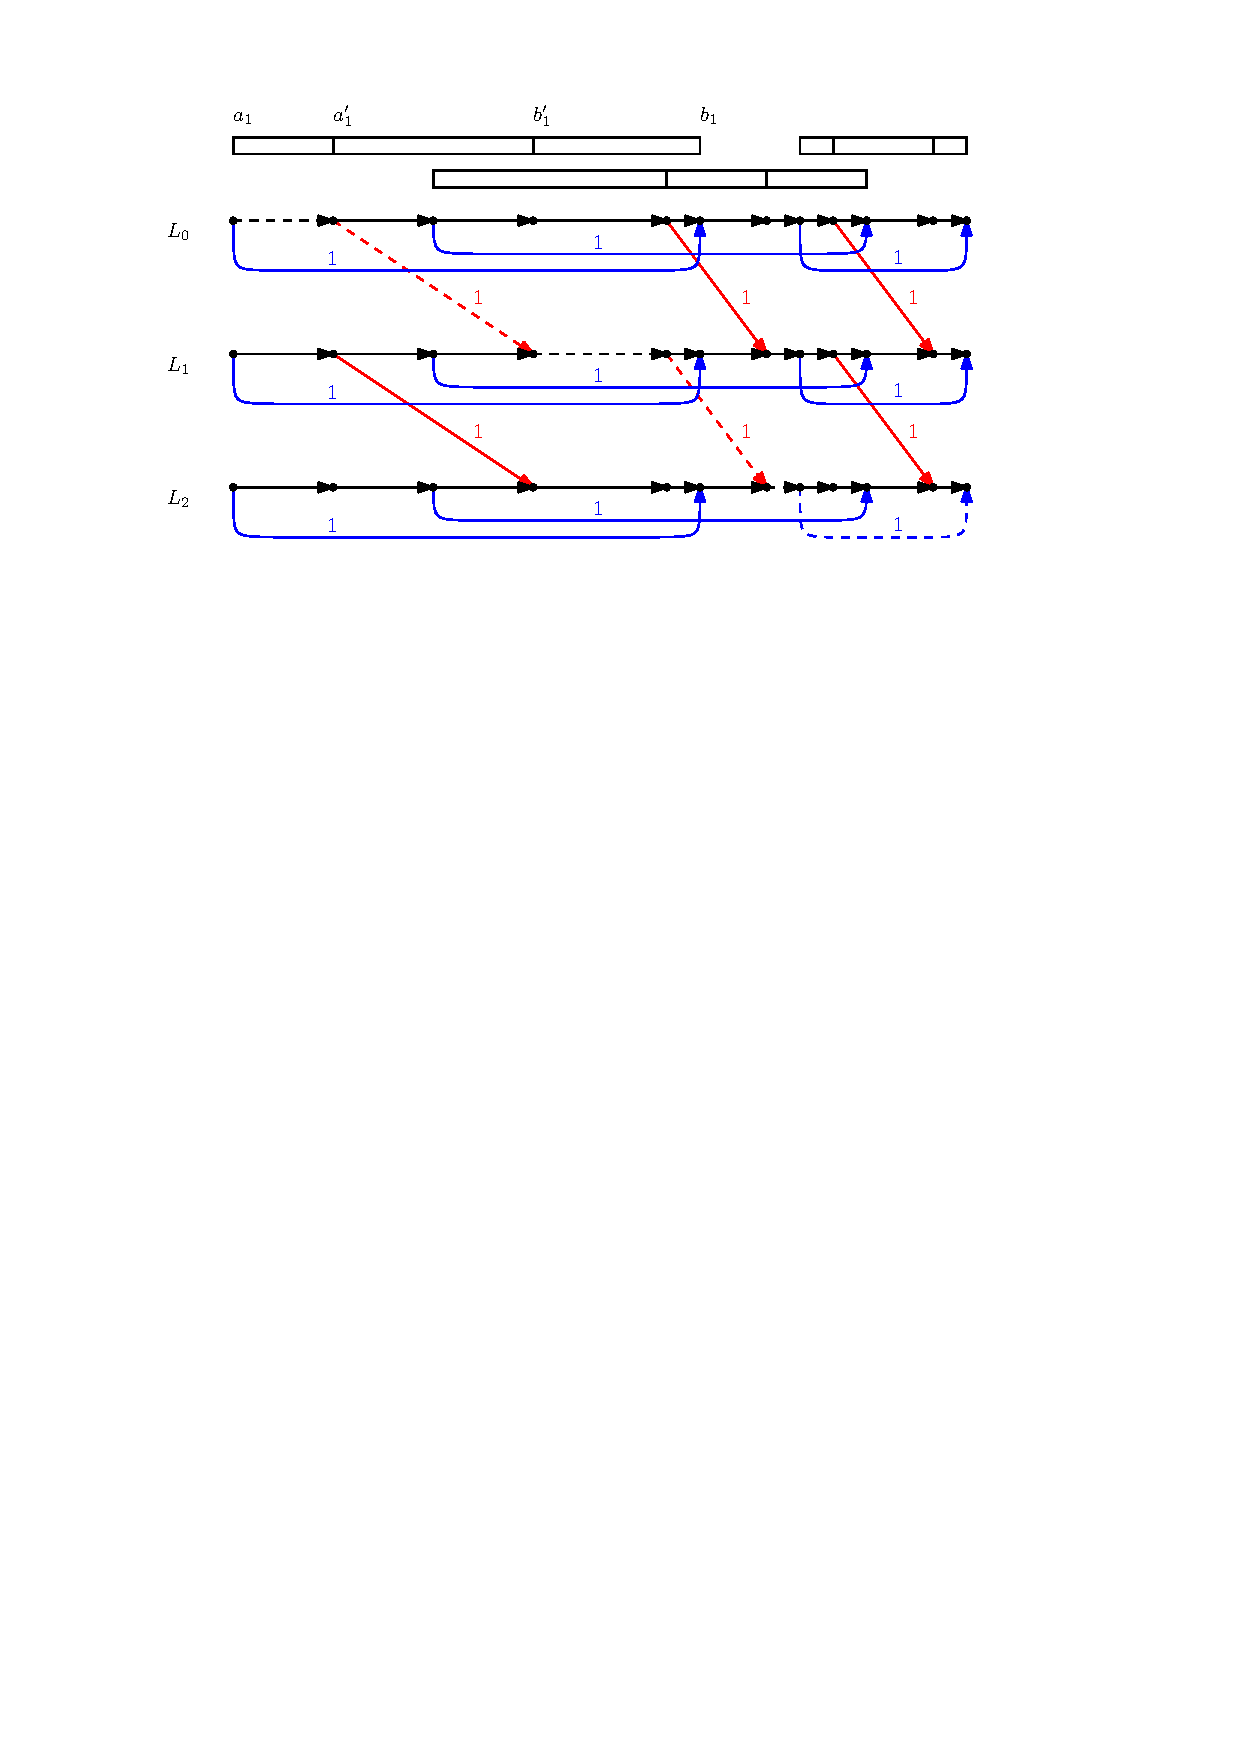
\includegraphics[width=\linewidth]{chapter-3-interdiction/figure_independent_set_assistance}
\caption{Illustration of the digraph used to solve the assistance problem for independent set. We have $n=3$ and $k=2$. 
The blue arcs correspond to the decision to add an interval from $\I$ to the solution and 
the red arcs correspond to the decision to add an interval from $\I'$ to the solution. To increase 
readability, all arcs of the form $(v_i^{\ell}, v_i^{\ell+1})$ are not drawn in the illustration.
The dotted edges correspond to an optimal solution for the given instance, where 
intervals $1$ and $2$ are \las{shrunk} and interval $3$ is selected without shrinking.}
\label{figure:indendent_set_assistance}
\end{figure}

The vertex set of $D$ consists of $k+1$ layers $L_0, \dots, L_k$. For each start- and endpoint $x \in \mathbb{R}$ of the intervals in $\I$ and $\I'$, we add $k+1$ vertices to $D$,
one in each layer $L_0$ up to $L_k$. For each such vertex $v$, we denote by $p(v) = x$ its corresponding point.
Let $v_1^{\ell}, \dots, v_{2n}^{\ell}$ be the vertices of layer $\ell$ ordered increasingly with respect to 
their corresponding point $p(v_i^{\ell})$ for all $i=1,\dots,2n$ and $\ell=0,\dots,k$.
We add arcs $(v_i^{\ell}, v_i^{\ell+1})$ of length zero to $D$ for all $\ell=0,\dots,k-1$ \hun{(omitted in \cref{figure:indendent_set_assistance} for readability)}.
We also add arcs $(v_i^{\ell}, v_{i+1}^{\ell})$ of length zero to $D$ for all $i=1,\dots,2n-1$ \hun{(black arcs in \cref{figure:indendent_set_assistance})}.
For each $i=1,\dots,n$ \hun{and for $i', j' \in [2n]$ such that} $p(v_{i'}^{\ell}) = a_i$ and $p(v_{j'}^{\ell})=b_i$, we add arcs 
$(v_{i'}^{\ell}, v_{j'}^{\ell})$ of length $1$ for all $\ell=0,\dots, k$ to $D$ (blue arcs in \cref{figure:indendent_set_assistance}). Note that traversing these arcs corresponds 
to adding $I_i$ to the solution. Also, for each $i=1,\dots,n$ \hun{and for $i', j' \in [2n]$ such that} $p(v_{i'}^{\ell}) = a'_i$ and $p(v_{j'}^{\ell})=b'_i$, we add arcs 
$(v_{i'}^{\ell}, v_{j'}^{\ell+1})$ of length $1$ for all $\ell=0,\dots,k-1$ to $D$ (red arcs in \cref{figure:indendent_set_assistance}). Note that traversing these arcs corresponds 
to adding $I'_i$ to the solution. In this DAG, we are now looking for a longest path from 
$s=v_1^1$ to $t=v_{2n}^k$. Given an $s$-$t$-path $P$ in $D$ we denote by $\I(P)$ 
the set of intervals corresponding to length-1 arcs selected.
Note that for each interval $F \in \I \cup \I'$ 
only one of the length-1 arcs corresponding to adding $F$ to the solution can be 
contained in an $s$-$t$-path, hence $\I(P)$ is well defined.

\begin{lemma}
    There exists an independent set $\J \subseteq \I \cup \I'$ such that 
    $ |\J \cap \I'| \leq k$ if and only if there exists an $s$-$t$-path $P$ 
    in $D$ such that $\I(P) = \J$ of length $|\J|$.
\end{lemma}
\begin{proof}
    All arcs of $D$ go from a vertex corresponding to a point $p$ 
    to a vertex corresponding to a point $p'$ where $p < p'$. In addition,
    all arcs of length $1$ go from the startpoint to the endpoint of the 
    interval that is added to $\I(P)$ if $P$ traverses the arc. Hence, given an
    $s$-$t$-path $P$ the length $1$ arcs traversed by $P$ correspond to 
    pairwise disjoint intervals from left to right, so the intervals $\I(P)$ form an 
    independent set. Also, observe that the number of intervals in $\I(P)$ that 
    are contained in $\I'$ is bounded by $k$, since every $s$-$t$-path can only 
    move from level $\ell$ to level $\ell+1$ once for all $\ell=0,\dots,k-1$.

    It is now easy to see that every independent set $\J \subseteq \I \cup \I'$ such that 
$ |\J \cap \I'| \leq k$ can also be converted into an $s$-$t$-path $P$ such that $\I(P) = \J$.
\qed\end{proof}

Based on this lemma, it holds that computing a longest path in $D$ is 
equivalent to solving the independence number \hun{interdiction} problem. By similar 
arguments as in the subsection above, the same algorithm can also be used to 
solve the clique cover number \hun{assistance} problem.
\hun{In addition, the longest path problem on an $n'$-vertex $m'$-edge directed acyclic graph can be solved in $O(m'+n')$ time~\cite{sedgewick2011algorithms}. 
It is easy to see that $D$ in the reduction above contains $O(kn)$ vertices and $O(kn)$ edges.}
In summary, we obtain the following result.

\begin{theorem}
    The independence number \las{assistance} and clique cover \las{interdiction} problem \las{in the shrink-expand framework} can 
    be solved in polynomial time.
    The algorithm can be implemented in $O(kn)$ time if we are given the lists of 
    intervals both sorted with respect to startpoints and endpoints.
\end{theorem}

\section{Maximum Clique Size}
In this section we consider the parameter $\omega$,
the maximum clique size of a graph. Note that for an interval graph $G$ it holds
that $\omega(G) = \chi(G)$, where $\chi(G)$ is the chromatic number of $G$.
The interdiction problem for $\omega$, which is equivalent to the assistance problem 
for $\chi$, has shrinking intervals, 
and the goal is to compute $\min_{|X| \leq k} \omega(G_X)$. 
The assistance problem for $\omega$, which is equivalent to the interdiction problem for $\chi$,
has expanding intervals, and the goal is to compute $\max_{|X| \leq k} \omega(G_X)$.

\subsection{Assistance problem}

\begin{theorem}\label{thm:clique:assistance}
    The maximum clique size assistance problem and the chromatic number interdiction problem \las{in the shrink-expand framework} can be solved in $\bigO(n)$ time, given the list of all intervals sorted with respect to endpoints. 
\end{theorem}
\begin{proof}
The problem is a highly local problem, since the maximum clique size is achieved at a point 
$x \in \mathbb{R}$ that is included in a maximum number of intervals.
Let $\fromto{p_1}{p_{2n}}$ be the set of all start- and endpoints of intervals in $\I \cup \I'$. For each $i \in [2n]$, let $\alpha_i$ be the number of intervals in $\I$ that contain $p_i$. Let $\beta_i := |\set{j \in [n] : p_i \not\in I_j, p_i \in I'_j}|$. The value $\beta_i$ is the maximum possible value by which $\alpha_i$ could increase by expanding some intervals. The set of all values $\alpha_i, \beta_i$ can be computed using a single sweep line algorithm. The solution to the assistance problem is then given by $\max_{i=1,\dots,2n} (\alpha_i + \min\set{\beta_i,k})$.
\qed\end{proof}



%We observe that for the case of maximum clique size and the chromatic number the operation of vertex deletion 
%can be modelled as a special case of the expansion operation in the shrink-expand framework, hence \autoref{thm:clique:assistance} 
%can be used to solve an assistance problem for chromatic number using the node deletion operation in polynomial time.
%\comment{Still doesn't make sense? Chromatic number assistance by vertex deletion = clique number interdiction by vertex deletion, was already handled by Diner et al.}
%\begin{corollary}
%    The assistance problem for the chromatic number on interval graphs with the node deletion operation can be solved in $\bigO(n)$ time.
%\end{corollary}
%\begin{proof}
%By setting $a'_i = -M, b'_i = M$ for all $i$ and a large enough constant $M$ 
%it holds that the expansion operation corresponds to connecting vertex $i$ to 
%all other vertices. Hence if $X \subseteq [n]$ and $|X|=k'$ it holds that 
%$\chi(G_X) = \chi(G-X) + k'$. Hence, by solving the interdiction problem for $k' = 0, \dots, k$ 
%one can obtain the solution to the most vital nodes problem for $\chi$.
%\todo{Shouldn't $k'$ be exactly $k$ here?}
%
%Note, that by modifying the proof of \autoref{thm:clique:assistance} 
%one can circumvent the need to to solve $k$ instances and obtain the linear running time.
%\qed\end{proof}

\subsection{Interdiction problem}

Diner et al.\ \cite{diner2018contractionDeletionBlockers} proved that the most vital nodes problem for maximum clique size on interval graphs can be solved in $\bigO(n)$ time with a simple greedy algorithm \cite{diner2018contractionDeletionBlockers}. 
Note that the most vital nodes problem for maximum clique size is a special case of the interdiction problem for maximum clique size in the shrink-expand framework 
by setting $a'_i = b'_i$ for all $i$. Observe that in this case the shrinking operation corresponds 
to the operation of removing all incident edges of a vertex, i.e. transforming it into a singleton. For 
the maximum clique size parameter this is equivalent to vertex deletion, except for the special case where $k=n$, which can be trivially handled.
In the general case (where we allow $a'_i \neq b'_i$), this problem becomes much harder. To show this, we reduce from the problem $\textsc{1-fold 2-interval cover}$. In this problem, we are given an integer $t \in \N$ and $n$ objects $O_1,\dots,O_n$, where every object $O_i = [x_{i1},x_{i2}] \cup [x_{i3}, x_{i4}]$ is a disjoint union of two intervals (a so-called \emph{2-interval}), such that $0 \leq x_{i1} < x_{i2} < x_{i3} < x_{i4} \leq t$. The goal is to decide whether there exists a selection of at most $k$ objects such that every $p \in \fromto{0}{t}$ is contained in at least one object of the selection. $\textsc{1-fold 2-interval cover}$ is NP-complete \cite{ding2011onefold} and W[1]-hard \cite{approximability-c-interval}.

\begin{theorem}
The maximum clique size interdiction problem and the chromatic number assistance problem in the shrink-expand framework is NP-complete. The problems are even W[1]-hard with respect to the parameter $k$.
\end{theorem}
\begin{proof}
Given an instance $(t, O_1, \dots, O_n)$ of $\textsc{1-fold 2-interval cover}$, we construct an instance of the maximum clique size interdiction problem. For each object $O_i$, we introduce a shrinking interval pair $[a_i, b_i] = [x_{i1}, x_{i4}]$ and $[a'_i, b'_i] = [x_{i2},x_{i3}]$. Let $\I := \fromto{[a_1, b_1]}{[a_n, b_n]}$ be the set of all $[a_i, b_i]$ introduced so far and let $M := \omega(\graph(\I))$ be the clique number of the corresponding interval graph. \hun{Then for each $p \in \fromto{0}{t}$, we iteratively} add additional \enquote{non-shrinkable} pairs $[a_{\hun{j}}, b_{\hun{j}}] = [a'_{\hun{j}}, b'_{\hun{j}}] = [p- \epsilon, p + \epsilon]$ for a small $\epsilon > 0$ \hun{and an unused index $j$}, until $p$ is contained in exactly $M + 1$ intervals. For this newly constructed instance, we have that the interdictor can reduce the clique number from $M + 1$ down to $M$ with a budget of $k$, if and only if there is a 1-fold 2-interval cover of $\fromto{0}{t}$ with at most $k$ objects.
\qed\end{proof}

%!TEX root = interval-interdiction-ciac.tex
% This is the version after considering empty intervals = isolated vertices

\newcommand{\scat}{\text{sc}}

\section{Scattering number, Hamiltonicity, and graph toughness}
\label{sec:hamiltonicity}
In this section, we \las{investigate the shrink-expand framework with respect to various parameters related to Hamiltonicity of an interval graph. All the problems considered in this section are of the same structure: As input we are given an interval graph in the shrink-expand framework with shrinking intervals. The given graph is Hamiltonian (or has a property similar to Hamiltonicity, like a Hamiltonian path, a small path cover, large graph toughness), and the question is whether the interdictor can destroy this property by shrinking at most $k$ intervals for a given budget $k$. In this section, we consider interdiction problems and most vital nodes problems with respect to Hamiltonian cycle, Hamiltonian path, path cover (\cref{subsection:ham_interdict,subsection:ham_mvn}), and graph toughness (\cref{subsection:tough}), as well as the assistance problem for scattering number (\cref{subsection:scat}). The formal definition of each of these problems is given at the beginning of the corresponding subsection. We show that each of these problems can be solved in polynomial time.}

\las{Before we begin, we have to introduce the concept of the \emph{scattering number}, which is crucially related to Hamiltonicity of interval graphs.}
We define by $c(G)$ the number of connected components in a graph $G$.
The scattering number of a graph $G$, denoted by $\scat(G)$, was defined by Jung~\cite{jung1978scat} as follows:

\[
    \scat(G) := \max \{c(G-S) - |S| : S \subseteq V(G) \text{ and } c(G-S) > 1\}.
\]
If the set above is empty, the graph $G$ is a complete graph, and in this case, we define $\scat(G) = -\infty$.

For an interval graph, the scattering number characterizes the Hamiltonicity of the graph, as summarized in the following theorem:

\begin{theorem}[Deogun, Kratsch, and Steiner~\cite{deogun1997scat}]
\label{thm:scat}
For an interval graph $G$ and for all constants $p \geq 1$,
\begin{itemize}
	\item $G$ contains a Hamiltonian path, if and only if $\scat(G) \leq 1$;
	\item $G$ contains a Hamiltonian cycle, if and only if $\scat(G) \leq 0$;
	\item $G$ contains a path cover of size $p$, if and only if $\scat(G) \leq p$.
\end{itemize}
\end{theorem}

One can easily see that the ``$\Rightarrow$" directions in the above theorem are true for any graph. In this section, we will prove the following theorem: (the formal definitions of the problems will be presented in the later subsections)

\begin{theorem}
\label{thm:ham}
In the shrink-expand framework, the following problems can be solved in time $\bigO(kn^3)$:
\begin{itemize}
	\item[(a)] The assistance problem for scattering number,
	\item[(b)] The interdiction problem for Hamiltonian path,
	\item[(c)] The interdiction problem for Hamiltonian cycle,
	\item[(d)] The interdiction problem for path cover,
\end{itemize}
\end{theorem}

As the scattering number is the central parameter in this section, we will first present the method to solve \las{the} assistance problem for scattering number in Section~\ref{subsection:scat}.
After that, we will show how by solving this problem, we can solve the interdiction problems mentioned in Theorem~\ref{thm:ham}.

We also discuss briefly two implications of the above theorem. 
Firstly, in Section~\ref{subsection:ham_mvn}, we show how the most vital nodes problem for Hamiltonicity parameters can be reduced to the assistance problem for scattering number and hence can be solved in similar time. 
Secondly, the method to solve the above assistance problem can be easily extended to the interdiction problem of a related parameter, graph toughness. 
In Section~\ref{subsection:tough}, we will define this parameter and discuss the modification needed to apply the method above to solve the latter problem. 

\subsection{Assistance problem for scattering number}
\label{subsection:scat}

The assistance problem for $\scat(G)$ is to compute $\max_{|X| \leq k}\scat(G_X)$ with shrinking intervals. 
In other words, we want to compute 

\begin{equation}
\label{eq:scat_assist}
  \max_{X \subseteq [n], |X| \leq k} \, \max_{S \subseteq [n], c(G_X - S) > 1} c(G_X - S) - |S|.
\end{equation}

We interprete problem (\ref{eq:scat_assist}) as a cooperative two-player game between an \emph{assistant} and the network owner. 
The assistant first selects the indices $\las{X \subseteq [n]}$ of the intervals to shrink, obtaining some graph $G_X$. 
After that, the network owner selects a set $\las{S \subseteq [n]}$ of vertices in $G_X$. 
The goal is that the property $c(G_X - S) > 1$ holds, and that under this condition, the value $c(G_X - S) - |S|$ is as large as possible.
\las{The goal of this subsection is to show that the optimal strategy of this game can be computed efficiently, i.e.\ we show that expression~(\ref{eq:scat_assist}) can be evaluated in polynomial time.
Since the argument is involved, we split it into several parts. We first briefly sketch the main idea without giving too many details.
After that, we introduce a certain important non-deterministic process used for the proof and explain the intuition behind it. Finally, we give a formal proof.}

\subsubsection{\las{The idea.}}

\las{We briefly sketch the main idea behind the proof. First, observe that we can w.l.o.g.\ assume that $X \cap S = \emptyset$. Indeed, whenever we have some number $i \in X \cap S$, it means that  the corresponding interval gets shrunk by the first player, and then deleted by the second player. But if a deletion occurs anyway, shrinking the interval is unnecessary for the goal of maximizing $c(G_X - S)$. This motivates}
 the following definition: A pair $(X,S)$ with $X, S \subseteq [n]$ is called a \emph{candidate pair}, if $|X| \leq k$ and $X \cap S = \emptyset$.
Further, we define 
\[
s(X,S) := \begin{cases} 
c(G_X - S) - |S| &\text{if } c(G_X - S) > 1,\\ 
-\infty &\text{otherwise.}
\end{cases}
\]
By the above explanations, we then have that the value of expression (\ref{eq:scat_assist}) is exactly 
\begin{equation}
 \max_{(X, S) \text{ candidate pair}} s(X, S). \label{eq:scat_assist_prime}
\end{equation}

\las{So it suffices to compute expression~(\ref{eq:scat_assist_prime}). How can we do that? 
We will introduce a non-deterministic process, which we call \emph{process $P$}. 
This process takes as input the instance $(\I, \I', k)$ and outputs some non-deterministically chosen value $\beta$. 
The idea behind this process $P$ is to mimic the cooperative game between the assistant and the network owner, but restrict it to certain rules, which preserve ``locality" during the process. 
The property that $P$ is non-deterministic corresponds to the fact that the two players have multiple choices during their game. 
The idea is that the output $\beta$ is ``the same" as the number $s(X,S)$, and so it is desirable to take those non-deterministic choices during a run of $P$ that maximize the output value $\beta$. 
 In the remainder of the subsection, we will first describe $P$ formally and provide an intuition for all its components. 
We will then prove our central lemma (\cref{lem:process_P}). It states that if $\beta_\text{max}$ is the maximum value that is returned by some run of $P$, then $\beta_\text{max}$ is equal to expression~(\ref{eq:scat_assist_prime}). 
Our second lemma (\cref{lem:ham_path}) states that $\beta_\text{max}$ can be computed in polynomial time using a dynamic program. Therefore, once we have proven these lemmas, we have shown that expressions~(\ref{eq:scat_assist_prime}) and (\ref{eq:scat_assist}) can be evaluated in polynomial time, as desired.}


\subsubsection{\las{The process $P$.}}

\SetKw{KwDownTo}{down to}
\SetKwBlock{KwBeginAA}{1a.)}{end}
\SetKwBlock{KwBeginAB}{1b.)}{end}
\SetKwBlock{KwBeginBA}{2a.)}{end}
\SetKwBlock{KwBeginBB}{2b.)}{end}
\SetKwBlock{KwBeginBC}{2c.)}{end}
\begin{algorithm}[htpb]
 \KwIn{Sequences $\I = ([a_1,b_1], \dots, [a_n,b_n])$ and $\I' = ([a'_1,b'_1], \dots, [a'_n,b'_n])$ s.t.\ $\forall i \in \set{1,\dots,n}: a_i \leq a'_i \leq b'_i \leq b_i \ $. Integer $k \geq 0$.}
 \KwOut{A non-deterministically chosen value $\beta$.}
 $\mathcal{F} = \I \cup \I' = \fromto{[c_1,d_1]}{[c_{2n},d_{2n}]}$ ordered by endpoint, i.e.\ $d_1 < d_2 < \dots < d_{2n}$ (w.l.o.g. $d_i \neq d_j$ for $i \neq j$). Let $F_i := [c_i, d_i]$ for $i \in \fromto{1}{2n}$.\;
 $k' \gets k$, $\gamma \gets 0$, $\beta \gets 0$\;
 $L \gets \emptyset$ \tcp*{stored using two variables, i.e. $L= [\ell, r]$}
\For{$i \gets 2n$ \KwDownTo $1$}{
	\eIf{$F_i \in \I$} {
		Let $t \in [n]$ s.t. $F_i = I_t$\;
		Choose non-deterministically exactly one of 1a.) or 1b.)\\
		\KwBeginAA{
			 $\textsc{lock}(I_t)$\; 
			\eIf{$I_t \cap L \neq \emptyset$}{
				$L \gets L \cup I_t$\;
			}
			{
				$L \leftarrow I_t$\;
				$\beta \gets \beta + 1$\;
				$\gamma \gets \min\{\gamma + 1, 2\}$\;
			}
		}
		\KwBeginAB{
			$\textsc{delay}(I_t)$\;
		}
	}
	{
		In this case we have $F_i \in \I'$. Let $t \in [n]$ s.t. $F_i = I'_t$. Choose non-deterministically exactly one of 2a.) or 2b.) or 2c.), subject to the constraints listed below.\\
		\KwBeginBA{
			Constraint: Only choosable if $I_t \subseteq L$\;
			$\textsc{lock}(I_t)$, $\textsc{discard}(I'_t)$\;
		}
		\KwBeginBB{
			Constraint: Only choosable if $I_t \not\subseteq L$\;
			$\textsc{delete}(I_t)$, $\textsc{discard}(I'_t)$\;
			$\beta \leftarrow \beta - 1$\;
		}
		\KwBeginBC{
			Constraint: Only choosable if $k' > 0$ and $I_t \not\subseteq L$\;
			$\textsc{shrink}(I_t)$, $\textsc{lock}(I'_t)$\;
			$k' \leftarrow k' - 1$\;
			\eIf{$I'_t \cap L \neq \emptyset$}{
				$L \gets L \cup I'_t$\;
			}
			{
				$\beta \gets \beta + 1$\;
				$\gamma \leftarrow \min\{\gamma + 1, 2\}$\;
				\lIf{ $I'_t \neq \emptyset$}{
					$L \leftarrow I_t'$ \label{algline:empty}
				}
			}
		}
	}
}
\leIf {$\gamma < 2$}{\KwRet{$- \infty$}}{\KwRet{$\beta$}}

 \caption{The non-deterministic process $P$.}
 \label{alg-chapter-4}
\end{algorithm}
%%%%%%%%%%%%----------------------
\las{Consider Algorithm~\ref{alg-chapter-4}, which provides a complete description of $P$ in pseudo-code. Before we proceed with the formal proof of our main lemmas, we explain in this paragraph the ideas behind process $P$ and its components.}

\las{Process $P$ receives as input an integer $k \geq 0$ together with sequences of intervals $\I = (I_1,\dots,I_n) = ([a_1,b_1], \dots, [a_n,b_n])$ and $\I' = (I'_1,\dots,I'_n) = ([a'_1,b'_1], \dots, [a'_n,b'_n])$, such that for all $i \in \set{1,\dots,n}$ we have $a_i \leq a'_i \leq b'_i \leq b_i$. We can assume w.l.o.g.\ that $a_i < b_i$ for all $i=1,\dots,n$. However, a special case that we cannot avoid is that for some indices $i$ it could be the case that $a'_i = b'_i$. Recall that we defined in the introduction that in this case we have $[a'_i, b'_i] = \emptyset$. (This definition may seem a bit unorthodox. However, it is crucial to correctly model the most vital nodes problem later in \cref{subsection:ham_mvn}.)
}

\las{After $P$ has received its input, it considers the union $\mathcal{F} := \I \cup \I'$ and orders it by the endpoints of the intervals, i.e.\ $\mathcal{F} = \fromto{F_1}{F_{2n}} = \fromto{[c_1,d_1]}{[c_{2n},d_{2n}]}$ such that $d_1 < d_2 < \dots < d_{2n}$ (we can w.l.o.g. assume that no two endpoints are equal). The main idea of $P$ is now to consider all the intervals $F_i$, starting with $i=2n$ and going down towards $i=1$, and making a partial decision about the fate of interval $F_i$. In particular, this decision is indicated by some keywords,  $\textsc{shrink}, \textsc{lock}, \textsc{delete}, \textsc{discard}, \textsc{delay}$. The meaning behind the keywords is as follows:}
Consider some index $t \in [n]$ and the pair of original interval $I_t$ and its replacement interval $I'_t$ with $I'_t \subseteq I_t$. 

\begin{itemize}
	\item[(i)] \las{Case 2c.) of the process: $\textsc{shrink}(I_t)$, $\textsc{lock}(I'_t)$ can be interpreted in the following way: It means that} the assistant \emph{shrinks} the original interval $I_t$ down to the replacement $I'_t$ and the network owner does \emph{not} delete the corresponding vertex $t$. We say that $I'_t$ gets \emph{locked}.
	\item[(ii)] \las{Case 2b.) $\textsc{delete}(I_t)$, $\textsc{discard}(I'_t)$ means that} the assistant does not shrink the original $I_t$, but the network owner \emph{deletes} the corresponding vertex $t$. We also say that the network owner \emph{deletes} $I_t$.
	\item[(iii)] \las{Case 1a.) or 2a.) $\textsc{lock}(I_t)$  means that the assistant decides not to shrink $I_t$, and the network owner decides not to delete the corresponding vertex $t$}.  We say that $I_t$ gets \emph{locked}. 
	\item[(iv)] \las{Case 1b.) $\textsc{delay}(I_t)$  means that neither the assistant nor the network owner want to decide on the fate of $I_t, I'_t$ right now. Instead the decision of what to do gets delayed into the future, when the process encounters $I'_t$. This option seems strange, but it turns out to be necessary in order to have a process with high ``locality".} 
	
\end{itemize}

\las{We will prove, that no interval is associated with two conflicting keywords, and every interval is associated with at least one keyword. This in turn implies that process $P$ can be understood as an alternative way to construct a candidate pair $(X, S)$.}
Note that for this pair $(X,S)$, the following holds: The interval representation of the graph $G_X - S$ consists of exactly those intervals $F \in \I \cup \I'$, for which $\textsc{lock}(F)$ has been called. In other words, locking an interval $F \in \I \cup \I'$ means committing to the final decision, that this interval will be part of (the interval representation of) $G_X - S$. 

\las{The concept of locking intervals is important for understanding the variable $L$. The variable $L$ is always an interval $L = [\ell, r]$, which is initially the empty interval. For the following explanation, we assume for the sake of simplicity that there are no indices $i$ with $a'_i = b'_i$.}
At each point in time $i = 2n, \dots, 1$ during the execution of $P$, let $R_i \subseteq \mathcal{F}$ be the set of \las{all the intervals in $\mathcal{F}$} that have been locked so far. The interval graph $\graph(R_i)$ has multiple components in general. Let $R_i' \subseteq R_i$ be the set of intervals corresponding to the leftmost component. \las{We will prove that process $P$} maintains two invariants: 
\begin{equation}
\label{eq:invariant_lock_in_alg}
L = \bigcup_{F \in R_i'}F \text{ and } r \geq d_i. 
\end{equation}
The first invariant essentially means that $L$ \las{at each point in time describes the space which the leftmost connected component of $G(R_i)$ occupies (note here that the union of intervals associated with one connected component in fact again is a single interval)}. The second invariant naturally follows the order of processing from largest endpoint to the smallest. \las{We remark that line~\ref{algline:empty} of the pseudo-code contains a special handling of the case where $a'_t = b'_t$. This special handling means that empty intervals do not interact with $L$.}

Finally, process $P$ \las{stores some variables in memory}, which are initialized at the start, and updated depending on the choices taken. One of these variables, $\beta$, will be such that its final value at the end of the process equals exactly $s(X, S)$. \las{This is because in line with the definition of $s(X,S)$, the variable $\beta$ is decreased every time we delete some interval, and increased every time we create a new connected component with the intervals $R_i$.} In addition, the process \las{stores} in memory a variable $k'$, which starts with value $k$ and describes the remaining budget of the assistant.
Finally, the process also keeps in memory a variable $\gamma$ that indicates $\min\{c(G(R_i)),2\}$.
In words, this variable keeps track of how many connected components are formed by the locked intervals so far.
Since at the end, we are only interested in whether the number of connected components is at least two, we cap the value of this variable at two.

\las{This completes our description of the process $P$.} Figure~\ref{fig:ham_path} contains an illustration of an execution of process $P$.
At the beginning, where $L = \emptyset$, we use the convention $\ell = r = \infty$. 
\begin{figure}
\centering
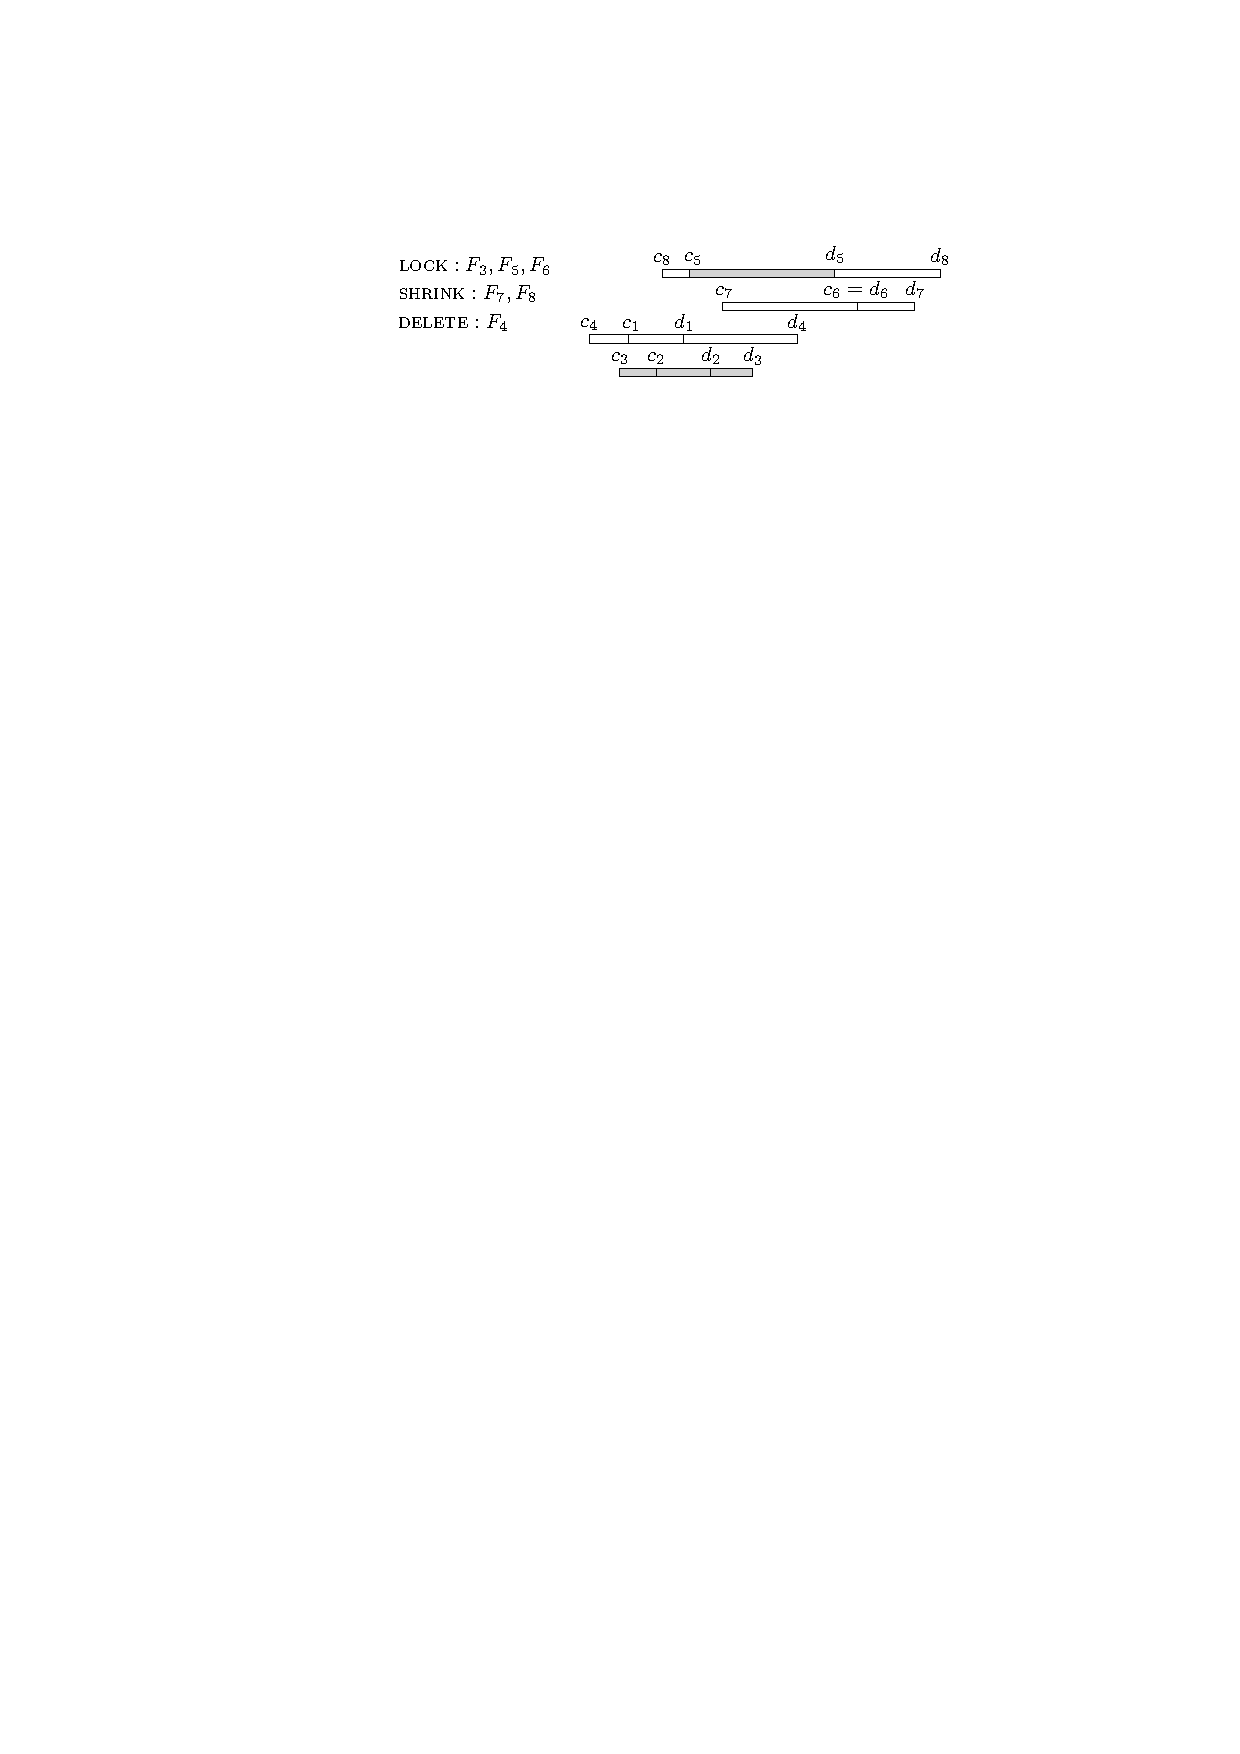
\includegraphics[scale=1]{chapter-3-interdiction/figure_ham_path}
\begin{tabular}{cl|ccccc}
    && \multicolumn{5}{c}{memstate after action}\\
    $i$ & \ action & $\ell$ & $r$ & $k'$ & $\gamma$ & $\beta$ \\ 
    \hline
    %------
    - & \ initialize & $\infty$ & $\infty$ & 2 & 0 & 0 \\
    8 & \ 1b.) $\textsc{delay}(F_8)$ & $\infty$ & $\infty$ & 2 & 0 & 0\\
    7 & \ 1b.) $\textsc{delay}(F_7)$ & $\infty$ & $\infty$ & 2 & 0 & 0\\
    6 & \ 2c.) $\textsc{shrink}(F_7)$, $\textsc{lock}(F_6)$ & $\infty$ & $\infty$ & 1 & 1 & 1\\
    5 & \ 2c.) $\textsc{shrink}(F_8)$, $\textsc{lock}(F_5)$ & $c_5$ & $d_5$ & 0 & 2 & 2\\
    4 & \ 1b.) $\textsc{delay}(F_4)$ & $c_5$ & $d_5$ & 0 & 2 & 2\\
    3 & \ 1a.) $\textsc{lock}(F_3)$ & $c_3$ & $d_5$ & 0 & 2 & 2\\
    2 & \ 2a.) $\textsc{lock}(F_3)$, $\textsc{discard}(F_2)$ & $c_3$ & $d_5$ & 0 & 2 & 2\\
    1 & \ 2b.) $\textsc{delete}(F_4)$, $\textsc{discard}(F_1)$ & $c_3$ & $d_5$ & 0 & 2 & 1\\
\end{tabular}
\caption{An example execution of process $P$: The top half shows the intervals, where each pair of enveloping intervals represents an original interval and its corresponding replacement. The locked, shrunken, and deleted intervals are listed on the left. The \las{table} shows the memory states \las{$(i,\ell,r,k',\gamma,\beta)$} throughout the process.}
\label{fig:ham_path}
\end{figure}



\begin{lemma}
\label{lem:process_P}
(i) For every sequence of choices one can take in process $P$, there exists a candidate pair $(X,S)$, such that the final value of $\beta$ equals $s(X, S)$.

(ii) For all candidate pairs $(X,S)$, there is a sequence of choices one can take in process $P$, such that at the end of the process, $\beta \geq s(X, S)$. 
\end{lemma} 
\begin{proof}
(i) Firstly, observe that for any execution of $P$, the invariants \las{(\ref{eq:invariant_lock_in_alg})} are maintained throughout the process. \las{This is because the variable $L$ is only changed in the cases 1a.) and 2c.), each of which maintains the invariants. (If we have the special case $a'_t = b'_t$ in case 2c.), the variable $L$ remains unchanged.)}
Secondly, we claim that at the end of process $P$, for every $I \in \I$, exactly one of the keywords $\textsc{shrink}(I)$, $\textsc{delete}(I)$, or $\textsc{lock}(I)$ was called. 
Indeed, when we process the interval $I$, if \las{1b.)} $\textsc{ delay}(I)$ is called, then when we process the corresponding replacement interval $I'$, exactly one of the above operations is called for $I$.
\las{On the other hand, suppose 1a.) $\textsc{lock}(I)$} is called when we process the interval $I$. \las{We have to prove that we do not associate a conflicting keyword (i.e.\ a keyword other than $\textsc{lock}$) with $I'$.}
Indeed, by the design of the process, $I \subseteq L$ after this step.
Due to \las{invariants~(\ref{eq:invariant_lock_in_alg})} and the fact that \las{$I' \subseteq I$ and due to the constraints of cases 2a.), 2b.) and 2.c), we have the following: At a later iteration,} right before process $P$ considers interval $I'$, we still have $I' \subseteq I \subseteq L$. \las{Again, due to the constraints, at this point in time the options 2b.) and 2c.) are forbidden and option 2a.) is available.}
Hence, the option \las{2a.)} $\textsc{ lock}(I), \textsc{discard}(I')$ \las{is} called.

Now consider an execution of process $P$ such that $\beta_0$ is the final value of the variable $\beta$.
We define \las{$X \subseteq [n]$ ($S \subseteq [n]$ respectively)} as the set of the indices such that \textsc{shrink} (\textsc{delete} respectively) has been called for the corresponding intervals. 
By the observation above, we have $X \cap S = \emptyset$.
Further, whenever we call the operation $\textsc{shrink}$, $k'$ is decreased by 1.
As $k'$ starts at $k$ and cannot go below 0 during the process, we have $|X| \leq k$.
Hence, $(X, S)$ is a candidate pair.

Consider the set $R_0$ of all intervals $F \in \mathcal{F}$ that were locked during the execution of $P$. 
%For a connected component in $\graph{F_i}$ that corresponds to an empty interval $I'_t$ for some $t \in [n]$, the process should have taken the option $\textsc{shrink}(I_t)$, $\textsc{lock}(I'_t)$ at the relevant point, and $\beta$ is increased by one then.
It is easy to see that each connected component of $\graph(R_0)$ corresponds to exactly one \las{iteration} in the execution of $P$, where $\beta$ was increased and vice versa. 
Indeed, if the component corresponds to an empty interval $I'_t$, this  was the iteration $i$, for which $F_i = I'_t$.
Otherwise, using invariants (\ref{eq:invariant_lock_in_alg}), \las{this iteration occurs when the variable $r$ is re-assigned to the} rightmost point of the component of $\graph(R_0)$. 
Clearly, the amount of times $\beta$ was decreased is exactly $|S|$.
Further, whenever $\beta$ is increased, we also increase $\gamma$ subject to the cap of 2.
Hence, if $\gamma$ is less than 2 after the process, $c(\graph(R_0)) \leq  1$ and $\beta$ is set to $-\infty$. 
Overall, we have $\beta_0 = s(X, S)$. 

(ii) Consider the following execution of the process $P$.
For each $t \in [n]$, when considering $I_t$, we choose the option \las{1a.) }$\textsc{lock}(I_t)$ if $t \notin X \cup S$ and the option \las{1b.) } $\textsc{delay}(I_t)$ otherwise.
When considering $I'_t$, we choose \las{2a.) }$\textsc{lock}(I_t), \textsc{discard}(I'_t)$ if possible.
\las{What do we do when choosing 2a.) is impossible?}  \las{Consider the constraints on options 2a.), 2b.) and 2c.) For a similar reasoning as in the previous paragraph, the fact that 2a.) is impossible for $I'_t$ implies that for the same index $t$ we did not choose option 1a.) when encountering $I_t$.} This implies that $t \in X$ or $t \in S$.
Because $(X,S)$ is a candidate pair, it is impossible that $t \in X \cap S$.
Then we choose $\textsc{shrink}(I_t), \textsc{lock}(I'_t)$ if $t \in X$ and $\textsc{delete}(I_t),$ $\textsc{discard}(I'_t)$ if $t \in S$.

Following the argument for the proof of (i) above, we can construct $X'$ and $S'$ such that the final value $\beta$ of the execution of $P$ equals $s(X',S')$. 
By construction, $X' \subseteq X$ and $S' \subseteq S$.
Further, following the above execution of the process $P$, it is easy to see that the intervals on the real line corresponding to the connected components of $G_X - S$ are the same as those for $G_{X'} - S'$.
Therefore, $c(G_{X'} - S') - |S'| \geq c(G_{X} - S) - |S|$, and hence $s(X',S') \geq s(X,S)$.
The lemma then follows.
 
\end{proof}

\begin{lemma}
\label{lem:ham_path}
The maximum possible value of $\beta$ at the end of process $P$ can be computed in time $\bigO(kn^3)$ by reduction to the maximum-cost path in a DAG.
\end{lemma}
\begin{proof}
An instance of the maximum-cost path in a DAG problem is a tuple $(H, \omega)$, where $H$ is a DAG and a function $\omega: E(H) \to \R$ describes the edge cost of $H$.
The problem is to find a path in $H$ with the maximum cost, which is defined as the sum of edge costs along the path.
This problem can be solved with dynamic programming with runtime linear to the number of edges \las{and vertices} of $H$ \las{\cite{sedgewick2011algorithms}}.

We first construct an instance of the maximimum-cost path in a DAG problem for the reduction. \las{Let $\mathcal{P} := \bigcup_{i=1}^{n}\set{a_i,b_i,a_i',b'_i}$.}
For every possible value assignments of $L = [\ell, r]$ (with \las{$\ell, r \in \mathcal{P}, \ell < r$}), every $k' \las{\in [k]}$, and $\gamma \in \set{1,2}$ describing the memory state of process $P$ at step $i \in \fromto{2n}{0}$, we add a vertex $(i,\ell,r,k',\gamma)$ in $H$. 
For $i \geq 1$, we create an edge from a vertex of the form $(i,\ell_1,r_1,k'_1,\gamma_1)$ to vertices $(i-1,\ell_2,r_2,k_2',\gamma_2)$, if and only if there is some possible choice in $P$ such that if the current memory state is $(i,\ell_1,r_1,k'_1,\gamma_1)$ then the new memory state would be $(i-1, \ell_2, r_2, k_2',\gamma_2)$ after this choice. 
Observe that the knowledge of $(i, \ell_1, r_1, k'_1,\gamma_1)$ suffices to determine which \las{of the choices 1a.), 1b.), 2a.) 2b.) and 2c.)} are possible and to determine the new memory state \las{(note that the interval $F_i$ can be derived from $i$)}. 
The edge costs are given by $+1$, if the line $\beta \leftarrow \beta + 1$ is called, by $-1$, if the line $\beta \leftarrow \beta- 1$ is called.
One exception is the step from a vertex $(1,\ell_1,r_1,k'_1,\gamma_1)$ to a vertex $(0,\ell_2,r_2,k'_2,\gamma_2)$, where $\gamma_2 < 2$.
In this case, we set the corresponding edge cost to $-\infty$.
The costs of all other edges are 0.

By construction, $H$ is a DAG, because for any edge in $H$, the first index of the starting vertex is higher than that of the ending vertex.
\las{Consider} a path connecting the starting vertex $(2n, \infty, \infty, k, 0)$ to a vertex $(0, \ell, r, k', \gamma)$. \las{By definition}, its cost is the final value \las{of} $\beta$ at the end \las{of} the execution of $P$ \las{which corresponds to that path}.
Consequently, the cost of the maximum-cost path is exactly the maximum possibe value of $\beta$ at the end of process $P$. 
There are $\bigO(n)$ possible values for each of $i, \ell, r$ respectively, so $H$ has $\bigO(kn^3)$ vertices and edges. Hence the desired path can be found in $\bigO(kn^3)$ time.
 
\end{proof}

\paragraph*{Proof of Theorem~\ref{thm:ham}(a).}
Let $\beta_{\max}$ be the maximum possible value of $\beta$ at the end of process $P$.
As a consequence of Lemma~\ref{lem:process_P}, there exists a candidate pair $(X,S)$ such that $s(X,S) = \beta_{\max}$, and
for any candidate pair $(X',S')$, there exists an execution of $P$ such that the final value of $\beta$ is at least $s(X',S')$.
This implies that $\beta_{\max}$ is the maximum of $s(X,S)$ over all candidate pairs $(X,S)$, i.e., the value of the original problem that we want to compute.
By Lemma~\ref{lem:ham_path}, $\beta_{\max}$ can be computed in time $\bigO(kn^3)$.
Theorem~\ref{thm:ham}(a) then follows.
 

\subsection{Interdiction problems for Hamiltonicity}
\label{subsection:ham_interdict}

In the interdiction problem for Hamiltonian path (cycle), we are given shrinking intervals $\I, \I'$, such that $\graph(\I)$ has a Hamiltonian path (cycle), and the interdictor wishes to select $X \subseteq [n]$ of size at most $k$, such that $\graph(\I_X)$ does not have a Hamiltonian path (cycle) anymore.
Similarly in the interdiction problem for path cover, we also have shrinking intervals, and the objective of the interdictor is to maximize the size of the path cover within the budget $k$ shrinkages.

\paragraph*{Proof of Theorem~\ref{thm:ham}(b)-(d).}
These are implied by Theorem~\ref{thm:scat} together with Theorem~\ref{thm:ham}(a).
To solve these problems, we first compute $\max_{|X| \leq k}\scat(G_X)$, i.e. the value of the assistance problem of the scattering number.
This value is also the value for the interdiction problem for path cover.
For the interdiction problems for Hamiltonian path and Hamiltonian cycle, we can conclude that the interdictor can interdict successfully, if and only if this value is more than 1 and 0 respectively.
Therefore, these problems can also be solved in time $\bigO(kn^3)$.
 

\subsection{Most vital nodes problem for Hamiltonicity}
\label{subsection:ham_mvn}
\las{In the most vital nodes problem for Hamiltonian path (cycle, respectively), we are given an interval graph, which has a Hamiltonian path (cycle, respectively) and a budget $k$. The question is whether the interdictor can destroy the property that the graph has a Hamiltonian path (cycle) by deleting at most $k$ vertices. More generally, the most vital nodes problem for path cover is to compute the number $\max_{X \subseteq V, |X| \leq k} \text{pc}(G - X)$, where $\text{pc}$ denotes the path cover number. We show that all these problems can be solved in polynomial time.}

Similar to other graph parameters discussed in this chapter, a natural question is whether the most vital nodes problems for Hamiltonian path, Hamiltonian cycle, and path cover are special cases of the shrink-expand framework.
The simple answer is no.
Here, shrinking to an empty interval and deleting a vertex yield different effect.
The former operation creates an isolated vertex and disconnects the graph, while the latter does not necessarily make the graph non-hamiltonian.

However, the most vital nodes problems for the above parameters can be reduced to the assistance problem for scattering number.
By Theorem~\ref{thm:scat}, the former problems can be immediately solved, if we know the value of the following problem $\textsc{Scat}(G,k)$: Given an interval graph $G$ and a budget $k$, what is the maximum scattering number that can be achieved after $k$ vertex \las{deletions}?
Note that this is technically not a most vital nodes problem in the traditional sense, as the goal of two players are aligned instead of conflicting.
The value of the problem $\textsc{Scat}(G,k)$ above in turn can be easily derived from the assitance problem for scattering number, as shown in the following lemma.

\begin{lemma}
Let $G$ be an interval graph and $k$ an integer.
Let $s_1$ be the value of the problem $\textsc{Scat}(G,k)$.
Let $s_2$ be the value of the assistance problem for scattering number with the budget $k$, where the original intervals are the intervals of $G$, and the replacement intervals are all empty intervals.
Then $s_1 = s_2 - k$.
\end{lemma}
\begin{proof}
Consider an optimal solution of $\textsc{Scat}(G,k)$.
There are $k' \leq k$ deleted vertices in this solution.
Replacing these vertices with empty intervals in the assistance problem yields a valid (but not necessarily optimal) solution with value $s_1 + k'$.
Since shrinking an interval always strictly increases the value of the scattering number, we shrink further $k - k'$ other intervals.
The value then becomes $s_1 + k$ and this is still a valid solution.
Hence, $s_1 + k \leq s_2$.

For the other direction, with the same observation that shrinking intervals always make the value better, there must exist an optimal solution of the assistance problem with exactly $k$ \las{shrunken} intervals.
We then delete these intervals in the problem $\textsc{Scat}(G,k)$, yielding a valid (but not necessarily optimal) solution with value $s_2 - k$.
Hence, $s_1 \geq s_2 - k$.

The lemma then follows. 
\end{proof}

Combining the above lemma with Theorem~\ref{thm:ham}(a), we obtain the following:
\begin{corollary}
The most vital nodes problem \las{on interval graphs} for Hamiltonian path, Hamiltonian cycle, and path cover can be solved in time $\bigO(kn^3)$
\end{corollary}

\subsection{Graph toughness}
\label{subsection:tough}
In this subsection, we will briefly discuss a related parameter, graph toughness, which was introduced by Chv\'{a}tal~\cite{Chvatal1973} as a measure of graph connectivity. 
A graph $G$ is $t$-tough if $|S| \geq t \cdot c(G - S)$ for any cutset $S$, i.e., $S \subseteq V(G)$ and $c(G - S) > 1$.
In the interdiction problem for graph toughness, we are given shrinking intervals $\I, \I'$, such that $G(\I)$ is $t$-tough, and the interdictor wishes to select $X \subseteq \I$ of size at most $k$, such that $G(\I_X)$ is not $t$-tough, i.e., we have
\[
	\max \{t \cdot c(G_X - S) - |S|  : S \subseteq \I_X \text{ and } c(G_X - S) > 1 \} > 0.
\]

If the set on the left-hand side is empty, then the graph $G_X$ is a complete graph and we define the maximum to be $-\infty$.

Observe that the left-hand side of the above expression is almost identical to the definition of scattering number, except for the factor $t$ in front of $c(G_X - S)$.
Therefore, we can adapt the method to solve the assistance problem for scattering number to solve this problem.
In fact, the only modification to the process $P$ is to replace all instances of $\beta \leftarrow \beta + 1$ by $\beta \leftarrow \beta + t$.
Effectively, each component now contributes $t$ instead of 1 toward the final sum.
Hence, following a completely analogous proof to the proof of Theorem~\ref{thm:ham}(a), we obtain the following:

\begin{corollary}
In the shrink-expand framework, the interdiction problem for graph toughness can be solved in time $\bigO(kn^3)$.
\end{corollary}


\section{Conclusion}
We have introduced a new framework of interdiction and assistance problems for interval graphs based on the shrinking and expanding operations.
In this framework, we have provided algorithms and classified the computational complexity of these problems for many classical parameters, including the shortest path, independence number, and clique number.
Except for the interdiction problem for the clique number which is NP-hard, the others are in P.
We have also formulated a polynomial-time algorithm for the assistance problem for the scattering number, which can be used to solve the interdiction problems for Hamiltonicity.
The interdiction problem for the scattering number, however, remains open.
We also noted that the most vital nodes problems of the above parameters are either special cases of the shrink-expand framework or can be easily solved by relevant problems in the framework. 
In particular, this has resolved an open problem posed by Diner et al.~\cite[(Q2)]{diner2018contractionDeletionBlockers}.

Finally, we note that our polynomial-time results do not generalize to superclasses of interval graphs: For the parameters $\alpha$ and $\omega$, Diner et al. proved that the most vital nodes problem is NP-complete on chordal graphs \cite{diner2018contractionDeletionBlockers}. It is also NP-complete to decide whether a chordal and bipartite graph has a Hamilton cycle \cite{muller1996hamiltonian}, so the most vital nodes problem is NP-complete too in this case. Finally, with respect to shortest path, the most vital nodes problem is NP-complete on general graphs \cite{complexityOfFindingMostVitalNodesShortestPath}, and the complexity on chordal graphs (to the best of our knowledge) is currently unknown. 

\section{Answer to question (Q1) by Diner et al.\cite{diner2018contractionDeletionBlockers}}
\label{app:contraction}

Let $G = (V, E)$ be a graph. For a set $X \subseteq E$, we denote by $G/X$ the graph obtained from $G$ by repeatedly contracting an edge from $X$, until no such edge remains. In \cref{sec:independence-interdiction}, we answered the open question (Q2) by Diner et al.\ \cite{diner2018contractionDeletionBlockers}. To do this, we used duality of the parameters of the independence number and the clique cover number. We show that using the same technique and a modification of the proof, we can also positively answer their question (Q1). The question is whether the \emph{contraction blocker} problem on interval graphs for parameter $\pi = \alpha$ can be solved in polynomial time. In this problem, one is given an interval graph $G = (V, E)$ and a threshold $t$, and wishes to find the minimum budget $k$, such that there exists $X \subseteq E$ of size $|X| \leq k$, such that $\alpha(G/X) \leq t$. By standard arguments, it suffices to solve the following problem instead: Given some budget $k \in \N$, compute
\begin{equation}
\min_{X \subseteq E, |X| \leq k}\alpha(G/X). \label{eq:contraction-problem}
\end{equation}  
We first show how to compute expression (\ref{eq:contraction-problem}) for connected interval graphs and then extend the answer to disconnected graphs. Like in \cref{sec:independence-interdiction}, let $\kappa(G)$ denote the clique-cover number of $G$. We also use the following notation in this section: We denote by $G = (V, E)$ some interval graph on $n$ vertices, with interval represention $\I = \fromto{[a_1, b_1]}{[a_n, b_n]}$. The set $\mathcal{B} =  \fromto{b_1}{b_n}$ is the set of all endpoints of intervals. Let $B \subseteq \mathcal{B}$. We call an interval $I \in \I$ \emph{disjoint from $B$}, if $I \cap B = \emptyset$. The following lemma establishes a connection between intervals disjoint to $B$ and problem (\ref{eq:contraction-problem}). Note that if $k = n$,  problem (\ref{eq:contraction-problem}) becomes trivial, so we can assume without loss of generality, that $k < n$.

\begin{lemma}
\label{lemma:contraction}
Let $G$ be a connected interval graph on $n$ vertices. If $k < n$, then
\begin{align*}
&\min_{X \subseteq E, |X| \leq k}\alpha(G/X) \\
= &\min\set{|B| : B \subseteq \mathcal{B}, \text{ at most $k$ intervals from $\I$ are disjoint from $B$}}.
\end{align*} 
\end{lemma}
\begin{proof}
\enquote{$\leq$}: Suppose there is a set $B$ such that at most $k$ intervals are disjoint from $B$. Note that not all intervals are disjoint from $B$, because $k < n$. So there exists at least one interval intersecting $B$ and at most $k$ intervals disjoint from $B$. We describe an edge contraction, which reduces the number of intervals disjoint from $B$: Assume there exists at least one interval disjoint from $B$. Then there exists also a pair of an interval $I$ disjoint from $B$ and an interval $J$ intersecting $B$, such that $I \cap J \neq \emptyset$. Otherwise the set of  intervals disjoint from $B$ and the set of intervals intersecting $B$ induce at least two connected components; a contradiction. Because $I \cap J \neq \emptyset$, there is a corresponding edge in $G$. Contracting this edge yields a new interval graph with interval representation $\I' := \I \setminus \set{I, J} \cup \set{I \cup J}$. Note that the number of intervals disjoint from $B$ in $\I'$ is one less than the number of intervals disjoint from $B$ in $\I$. Therefore, we can repeat this procedure at most $k$ times, to obtain an edge set $X \subseteq E$ of size $|X| \leq k$, and an interval representation $\I''$, such that no interval in $\I''$ is disjoint from $B$ and $G/X = \graph(\I'')$. Using duality of $\alpha$ and the clique cover number $\kappa$, and the fact that no interval in $\I''$ is disjoint from $B$, we have
\[\alpha(G/X) = \kappa(G/X) = \kappa(\graph(\I'')) \leq |B|.  \]

\enquote{$\geq$}: Let $X \subseteq E$ with $|X| \leq k$, and let $\alpha(G/X) = t$. Then also $\kappa(G/X) = t$, so there exists a clique cover with $t$ cliques $C_1, \dots, C_t$. By \cref{prop:cliquecover}, each of the $t$ cliques is equal to (or contained in) the set $C(b)  \las{ := } \set{I \in \I : b \in I}$ for some $b \in \mathcal{B}$. Let $b'_1, \dots, b'_t$ be the corresponding $t$ points, such that $C_i \subseteq C(b'_i)$ for all $i = 1,\dots,t$. Let $B := \fromto{b'_1}{b'_t}$. We can now reverse the edge contractions, going from $G/X$ to $G$, and observe that each decontraction adds at most one interval disjoint to $B$. Hence, $B$ is a set of size $t$, such that at most $k$ intervals in $\I$ are disjoint to $B$. \qed
\end{proof}

\begin{theorem}
\label{thm:contraction-blocker}
Given an interval graph $G$ on $n$ vertices and $k \in \N$, problem (\ref{eq:contraction-problem}) can be computed in $\bigO(kn^2)$ time.
\end{theorem}
\begin{proof}
We distinguish three cases:

\textbf{Case 1:} $G$ is connected, and $k \geq n$. Then \cref{eq:contraction-problem} evaluates to 1.

\textbf{Case 2:} $G$ is connected, and $k < n$. Let $\mathcal{B} = \fromto{b_1}{b_n}$ be the set of endpoints, such that w.l.o.g.\ $b_1 < b_2 < \dots < b_n$. Additionally, let $b_0 := -\infty$ and $b_{n+1} := \infty$. For $i,j \in \fromto{0}{n+1}$ and $i < j$, let 
\[c(i, j) = |\set{k \in [n] : b_i < a_k < b_k < b_j}|. \]
Note that $c(i, j)$ is the number of intervals between $b_i$ and $b_j$ disjoint to $\set{b_i, b_j}$. It is easy to see that the set of all values $c(i,j)$ can be computed in $\bigO(n^2)$ time.


We define for $j \in \fromto{1}{n+1}$ and $k' \in \fromto{0}{k}$:
$F(j, k')$ is the minimum size of a set $\las{B} \subseteq \fromto{b_1}{b_j}$ subject to $b_j \in B$, and at most $k'$ intervals in $\fromto{[a_1,b_1]}{[a_j, b_j]}$ are disjoint to $B$. Furthermore, define $F(0, k') = 0$ for all $k'$. It is then easy to see that 
\begin{equation}
F(j,k') = \min \{ 1 + F(i, k'-c(i,j)) \colon 0 \leq i < j\text{ and } c(i,j) \leq k' \}.
\end{equation}  
Finally, due to \cref{lemma:contraction}, we have that 
\[\min_{X \subseteq E, |X| \leq k}\alpha(G/X) = F(n+1, k) - 1. \]
(Note that the $-1$ comes from the fact that $F(n+1, k)$ counts the point $b_{n+1}$.)

\textbf{Case 3:} $G$ is disconnected. Assume $G$ consists of \las{connected} components $C_1, \dots, C_{\ell}$, where component $C_i$ has $n_i$ vertices. The interdictor needs to distribute the budget $k = k_1 + \dots + k_{\ell}$ to the $\ell$ components. By the above argument, we can precompute in time $\bigO(kn_i^2)$ a table of all the values $\min_{|X| \leq k_i} \alpha(C_i/X)$ for $k_i \in \fromto{1}{k}$. The interdictor now needs to solve 
\[ \min_{k = k_1 + \dots + k_{\ell}} \sum_{i=1}^{\ell} \min_{|X| \leq k_i} \alpha(C_i/X). \]
It is an easy exercise to prove that this formula can be evaluated in time $\bigO(k\ell)$ using dynamic programming. In total, we have a running time of $\bigO(\sum_i kn_i^2 + k\ell) = \bigO(kn^2)$. \qed
\end{proof}

\begin{corollary}
The contraction blocker problem on interval graphs for parameter $\pi = \alpha$ can be solved in time $\bigO(n^3)$.
\end{corollary}
\begin{proof}
Running the algorithm in \cref{thm:contraction-blocker} for $k = n$, we obtain a dynamic programming table containing for each $k' \in \fromto{1}{n}$ the maximum possible effect the interdictor can achieve with a budget of $k'$. Using binary search, we can find the minimum budget $k'$ necessary to reduce $\alpha$ down to the threshold $t$.
\end{proof}


\chapter{A Linear Time Algorithm for Linearizing Quadratic and Higher-Order Shortest Path Problems}
\label{ch:linearization-2}


%\numberwithin{equation}{section}

%Special short commands for interval interdiction notation

\section{Introduction}\label{intro:sec}

Just like the last chapter, this chapter deals with the linearization problem for 
nonlinear
generalizations of the  \emph{Shortest Path Problem (SPP)}. We recall the relevant definitions.
An instance of the SPP  consists  of a digraph $G = (V, A)$,  a source vertex $s \in V$, a sink vertex $t \in V$, and a
cost function $c\colon A\to \rz$, which maps each arc $a\in A$ to its cost
$c(a)$.  The cost of a simple directed $s$-$t$-path $P$, 
is given by\footnote{We use the same  notation for the path $P$ and the set of its arcs.}
\begin{equation}\label{SPP:obj}  \text{SPP}(P,c):=\sum_{a\in P} c(a)\, .  \end{equation}
The goal  is to find a simple directed 
$s$-$t$-path in $G$ which minimizes the objective 
(\ref{SPP:obj}).
In general it is assumed that 
there are no circuits of negative weight in $G$. 


Unlike in the last chapter, in this chapter we are concerned with cost functions of possibly even higher order than 2. Consider a number $d\in \N, d \geq 2$.  The \emph{Order-d Shortest Path Problem
  (SPP$_d$)}
 takes as input a  digraph $G = (V, A)$,  
  a source vertex $s \in V$, a sink vertex $t \in V$, and an order-$d$ arc interaction 
cost  function $q_d\colon \set{B \subseteq A : |B| \leq d}
\to \rz$. Thus $q_d$ assigns a  weight to every subset of
arcs of cardinality at most $d$.
 The cost of a simple directed $s$-$t$-path $P$ 
is given by
\begin{equation}\label{dSPP:obj}
  \text{SPP}_d(P,q_d):=\sum_{S\subseteq P \colon |S|\le d} q_d(S)\, .\end{equation}
The goal is to find  
a simple directed 
$s$-$t$-path in $G$ which minimizes the objective function (\ref{dSPP:obj}).
For $d=2$ we
obtain the   \emph{Quadratic  Shortest Path Problem (QSPP)} which has been introduced in the last chapter. We remark that the notation in this chapter is slightly different, since we are interested in generalizations to $d > 2$. However, the two notations can be easily seen to describe the same problem. We recall that the QSPP has been studied extensively in the literature
~\cite{cela2021linearizable,huSo2018,huSo2020,rostami2018}. 


\smallskip

The QSPP arises 
in network optimization  problems where costs are associated with both single arcs and pairs of arcs.
This includes 
variants of stochastic and time-dependent route planing  problems  
\cite{nie2009reliable,sen2001mean,sivakumar1994variance}
and network design problems 
\cite{murakami1997restoration,gamvros2006satellite}. 

For an overview of applications of the QSPP see \cite{huSo2020,rostami2018}.
We are not  aware of any
publications  
for the case $d>2$.


While the SPP can be solved in polynomial time, the QSPP is an NP-hard
problem even for the special case of the adjacent QSPP where  the  costs of all pairs of non-consecutive  arcs are  
zero ~\cite{rostami2018}.
The QSPP is  an  extremely difficult
problem also from the practical point of view.  
 Hu and Sotirov~\cite{huSo2020} report that a state-of-the-art quadratic solver can
solve QSPP instances with up to $365$ arcs, while their  tailor-made B\&B
%branch and
%bound 
algorithm can solve instances with up to $1300$ arcs to optimality within one  hour. 
Instances of the SPP can however be solved in a fraction of a second for graphs with
millions of vertices and arcs.

\smallskip

Given the 
hardness of the QSPP, a research line on this problem has focussed
on 
polynomially solvable special cases which
arise if the input graph and/or the cost coefficients have certain specific
properties. Rostami et al.~\cite{rostami2015} have presented a polynomial time
algorithm for the adjacent QSPP in acyclic digraphs and in series-parallel graphs. Hu 
and Sotirov~\cite{huSo2018}
have shown that the QSPP can be solved in polynomial time if the  quadratic
costs build a  nonnegative symmetric product matrix, or if the quadratic costs
build a sum matrix and all $s$-$t$-paths in 
$G$ have the same number of arcs. 
These two polynomially solvable
special cases of the QSPP belong to the larger class of the \emph{linearizable $\text{SPP}_d$ instances} defined as follows.
\begin{definition}
\label{def:linearizable}
 An instance of the SPP$_d$ with an input digraph $G=(V,A)$, a source node $s$, a sink node $t$
 and a  cost function $q_d$ is called linearizable if there exists a cost function
 $c\colon A\to \rz$ such that for any simple directed $s$-$t$-path  $P$ in $G$ the equality
 $\text{SPP}(P,c) = \text{SPP}_d(P,q_d)$ holds.
 %\todo{BK: Slight change of this sentence. We could also omit it alltogether}
  %A linearizable instance  of the  QSPP is defined analogously, just  replacing %$\text{SPP}_d(P,q_d)$ by $\text{QSPP}(P,q)$.
  A linearizable instance  of the  QSPP is a linearizable instance of the $\text{SPP}_2$.
  %defined analogously, just  replacing $\text{SPP}_d(P,q_d)$ by $\text{QSPP}(P,q)$.
\end{definition}

The recognition of linearizable QSPP (SPP$_d$) instances, also
called \emph{the linearization problem for the QSPP (SPP$_d$)}, abbreviated by \textsc{Lin}QSPP (\textsc{Lin}SPP$_d$) arises 
as a natural question. In this problem the task 
consists of deciding whether a
given  instance of the  QSPP (SPP$_d$)  is linearizable and in finding the linear cost function
$c$ in the positive case.
The 
notion of 
linearizable special cases of hard
combinatorial optimization problems  goes back to
 Bookhold~\cite{bookhold1990contribution} who introduced 
 it for  the quadratic assignment problem (QAP). 
 For symmetric linearizable QAP instances a full characterization has been obtained while
 only partial results are available for the linearizability of the general QAP, see
 \cite{CeDeWo2016,Erdogan2006,ErTa2007,ErTa2011,kabadi2011n,punnen2013linear,waddellcharacterizing}.
The linearization problem has been studied for several other quadratic combinatorial optimization problems, see  \cite{CuPu2018,sotirov2021quadratic}
for the quadratic minimum spanning tree problem,  \cite{PuWaWo2017} for the quadratic TSP, \cite{deMeSo2020} for the quadratic cycle cover problem and  \cite{huSo2021} for general binary quadratic programs.  
Linearizable instances of  a quadratic problem can be used  to generate lower bounds  needed   in B\&B algorithms. For example, Hu and Sotirov introduce the family of the so-called \emph{linearization-based bounds} \cite{huSo2021} for the binary quadratic problem. Each specific bound of this family is based on   a set of linearizable instances of the problem. The authors show that 
well-known bounds from the literature are special cases of the newly introduced bounds.
Clearly, fast algorithm for the  linearization problem are important in 
this context.
\smallskip

While \textsc{Lin}SPP$_d$ has not been investigated in the literature so far (to the best of our knowledge), the  \textsc{Lin}QSPP has been subject of investigation in some recent papers.
In the last chapter, it was proven  that it  is  coNP-complete to decide whether a   QSPP instance on an   input graph
containing   a directed cycle is linearizable.    Thus, a nice characterization of linearizable QSPP
  instances for such  graphs
  seems to be
  unlikely.
   In the acyclic case, Hu and Sotirov first described a polynomial-time
   algorithm for the \textsc{Lin}QSPP  on  directed
   two-dimensional grid graphs \cite{huSo2018}. Recently, in  \cite{huSo2021} they  generalized this
   result to all acyclic digraphs and proposed  an algorithm which solves the
   problem in $\bigO(nm^3)$, where $n$ and $m$ denote the number of vertices and
   arcs in 
   $G$.
\smallskip
   
   We recall that in the last chapter, the  so-called universal linearizability was studied.
A digraph $G$ is called \emph{universally linearizable with respect to the
  QSPP} iff every instance of the QSPP on the input graph $G$ is linearizable for
every choice of the cost function $q$. In \cite{huSo2018} it is shown that a
particular class of grid graphs is universally linearizable. In
the last chapter, we obtained several different complete characterizations of the class of universally linearizable digraphs, for example in terms of 
forbidden subgraphs.  
\medskip

\textbf{Contribution and organization of the chapter.}
In this chapter we provide a novel and simple characterization of linearizable QSPP instances on acyclic 
digraphs.
Our characterization shows that the linearizability can be seen as a  \emph{local} property.  In particular, we show  that an instance of the QSPP on an acyclic 
digraph $G$  is linearizable if and only if each subinstance obtained by considering a subdigraph of $G$ consisting of two $s$-$t$-paths in $G$   is linearizable. Our simple characterization also works for the SPP$_d$  and even for completely arbitrary cost  functions, which  assign some cost $f(P)$ to every $s$-$t$-path $P$ without any further restrictions. The latter problem is referred to as the \emph{Generic Shortest Path Problem} (GSPP) and is formally introduced in Section~\ref{defi:sec}. Indeed, the characterization of the linearizable instances of the SPP$_d$ 
follows from the characterization of the linearizable instances of the GSPP, both on acyclic digraphs. We remark that in parallel and independent to our work, Matuschke proved an equivalent result \cite[Theorem 6]{matuschke2023decomposition}.

Further,  we propose  a 
linear time algorithm
which can check the local condition mentioned above   for the QSPP and the SPP$_d$. 
We note that this is not straightforward, because the number of the subinstances for which the condition needs to be checked is in general exponential. As a side result our approach reveals  an interesting connection between the \textsc{Lin}QSPP and the problem of deciding  whether all $s$-$t$-paths in a digraph have the same length.
As a result, we obtain an algorithm which solves the \textsc{Lin}QSPP  in $\bigO(m^2)$ time, thus improving the best previously known running time of $\bigO(nm^3)$ obtained in \cite{huSo2021}. Our approach yields an $\bigO(d^2 m^d)$ time algorithm for the \textsc{Lin}SPP$_d$, thus providing  the first (polynomial time) algorithm for this problem.  Note that the running time of the proposed algorithms is linear in the input size for both problems,  \textsc{Lin}QSPP and \textsc{Lin}SPP$_d$, respectively. 
(The costs of all $\Omega(m^2)$ pairs of arcs, in the case of the QSPP, and the  costs of all $\Omega(m^d/d!)$ subsets of  arcs of cardinality $d$, in the case of the
SPP$_d$,  need to be encoded in the input.) 


Finally, we also obtain a polynomial time algorithm that given an acyclic digraph $G$ computes a basis of the subspace of all linearizable degree-$d$ cost functions on $G$. Such a basis can be used to obtain better linearization-based bounds usable in B\&B algorithms.

The chapter is organized as follows. 
After introducing some notations and preliminaries in Section~\ref{defi:sec} we present the result on the characterization of the linearizable QSPP and SPP$_d$ instances on acyclic input digraphs in Section~\ref{charact:sec}. The algorithms for the linearization problems \textsc{Lin}QSPP and \textsc{Lin}SPP$_d$ are presented in Section~\ref{algo:sec}. 
%In \cref{sec:subspace} we give a polynomial time algorithm computing a basis %of the subspace of all linearizable $d$-degree cost functions on an acyclic digraph $G$.
\cref{sec:subspace} deals with 
%we give a polynomial time algorithm 
computing a basis of the subspace of all linearizable $d$-degree cost functions on an acyclic digraph $G$.

\section{Notations  and preliminaries}\label{defi:sec}

 Given a digraph $G=(V,A)$, a simple directed $s$-$t$-path $P$ in $G$ is specified as a sequence of
arcs $P=(a_1,a_2,\ldots,a_p)$ such that  $a_1$ starts at $s$, $a_p$
ends at $t$, nonconsecutive arcs do not share a vertex and  the end vertex of $a_{i}$ coincides with  the start vertex of $a_{i+1}$ for any $i\in \{1,\ldots,p-1\}$. The number
$p$ of arcs in $P$ is called the length of the path. We sometimes use the same notation for a path $P$ and the  set of its arcs. 
%Alternatively, a simple directed $s$-$t$-path $P$ of length $p$ in $G$  is specified as a sequence of pairwise disjoint vertices $(u_0,u_1,\dots,u_p)$, 
%where $x_0=s$, $u_p=t$ and $(u_i,u_{i+1})\in A$ for all $i\in\{0,\dots,p\}$. Thus  $a_i=(u_{i-1},u_i)$, for $i\in \{1,\dots,p\}$. 
We  consider a single arc $(x, y)$ as an $x$-$y$-path of length $1$  and a single vertex $x$ as a  trivial $x$-$x$-path of length $0$. Given an  $x$-$y$-path $P_1$ and a  $y$-$z$-path $P_2$, we denote the \emph{concatenation} of $P_1$ and $P_2$ by $P_1 \cdot P_2$. We also consider concatenations of paths and arcs, that is, terms of the form $P \cdot a$ for some $x$-$y$-path $P$ and some arc $a = (y, z)$.
 
In the linearization problem, we are concerned with acyclic digraphs $G =(V, A)$ with a source vertex $s$ and a sink vertex $t$. 
We denote by  $\Pst$ the set of all simple directed $s$-$t$-paths.
We often assume that $G$ is \emph{$\Pst$-covered}, that is, every arc in $G$ is traversed by at least one path in $\Pst$. 
Note that we can make this assumption without loss of generality: If some arc is not traversed by at least one $s$-$t$-path, then it has no effect on the linearizability of the instance, and so we can delete that arc.

Let $d \geq 2$ be a natural number. The \emph{Order-$d$ interaction costs} are given by a mapping $q_d\colon \set{B \subseteq A : |B| \leq d}\to \rz$, assigning a (potentially negative) interaction cost to every subset of at most $d$ arcs.
The cost $\text{SPP}_d(P,q_d)$ of some path $P$ under interaction costs $q_d$ is defined as in equation (\ref{dSPP:obj}).
If $d$ is unambiguously clear form the context, we use the  more compact notation $f_q(P): = \text{SPP}_d(P,q_d)$.
 In this chapter we explicitly allow the case $q(\emptyset) \neq 0$, because this simplifies the calculations.  
The \emph{linearization problem for the Order-$d$ Shortest Path Problem} (\textsc{Lin}SPP$_d$)
is formally defined as follows.
\begin{center}
%%%%%%%%%%%%%%%%%
\boxxx{\textbf{Problem:} The  linearization problem for the SPP$_d$ (\textsc{Lin}SPP$_d$)
\\[1.0ex]
\textbf{Instance:} A $\Pst$-covered directed graph $G=(V,A)$ with $s,t\in V$, $s\neq t$; an integer $d \geq 2$;
an order-$d$ arc interaction cost function $q_d: \set{B \subseteq A \colon |B| \leq d} \to \R$.
\\[1.0ex]
\textbf{Question:} Find a \emph{linearizing cost function}  $c\colon A\to\R$  such that $\text{SPP}_d(P,q_d) = \text{SPP}(P,c)$ for all $P \in \Pst$ or decide that such a linearizing  cost function does not exist.}
%%%%%%%%%%%%%%%%%
\end{center}
%%%%%%%%%%%%
In the special case $d = 2$, we obtain the    linearization problem for the QSPP (\textsc{Lin}QSPP).
\smallskip

Finally, let us consider the \emph{Generic Shortest Path Problem} (GSPP) which takes as input  a digraph $G=(V,A)$ with a source vertex $s$, a sink vertex $t$, $s\neq t$, and a generic cost function $f\colon \Pst \to \rz$  assigning  a cost $f(P)$ to every path $P\in \Pst$\footnote{We assume that $f$ is specified by an oracle.}. We assume w.l.o.g.\ that $G$ is $\Pst$-covered. The goal is to find an $s$-$t$-path  which minimizes the objective function $f(P)$ over $\Pst$. 
A linearizable instance of  the GSPP and the linearization problem for the GSPP (\textsc{Lin}GSPP) are  defined analogously as in the respective definitions for SPP$_d$.



We note that in our \cref{def:linearizable} we allowed the case that the linearizing function $c : A \to \R$ can take negative values. This could be a problem, since if a digraph contains negative cycles, the shortest path problem is NP-hard in general. However, as we are only concerned with acyclic digraphs in this chapter, this is not a problem. In fact, the following lemma shows that for acyclic digraphs it is a more difficult problem to decide if there is a linearizing function $c : A \to \R$ than the problem to decide if there is a linearizing function $c': A \to \R_+$. Hence, we consider only the first problem for the rest of the chapter.
\begin{lemma}
If $(G,s,t,f)$ is an instance of the GSPP such that $G  = (V,A)$ is an acyclic digraph, then there is a nonnegative linearizing function $c' : A \to \R_+$ if and only if there is a linearizing function $c : A \to \R$ and $f(P) \geq 0$ for all $s$-$t$-paths $P$.
\end{lemma}
\begin{proof}
If there is no linearizing function $c : A \to \R$, then in particular there is also no linearizing function $c' : A \to \R_+$. On the other hand, if there is a linearizing function $c : A \to \R$, then we distinguish two cases. If there is an $s$-$t$-path $P$ with $f(P) < 0$, then clearly there cannot exist a linearizing cost function  $c' : A \to \R_+$, because $P$ would receive the incorrect costs $c'(P) \geq 0$. On the other hand, if $f(P) \geq 0$ for all $s$-$t$-paths, we claim that we can find nonnegative $c'$ as desired. Indeed, for all vertices $v \in V$, we let $\pi(v)$ be the cost of a shortest $s$-$v$-path with respect to $c$. Since $G$ has no cycles, in particular no negative cycles we have that for all arcs $(u,v) \in A$ the inequality $\pi(v) \leq \pi(u) + c(u,v)$ holds. We define the adjusted costs $c_\pi(u,v) := \pi(u) - \pi(c) + c(u,v)$ for all arcs $(u,v) \in A$. By the previous inequality we have $c_\pi(u,v) \geq 0$. By a telescope argument we have $c_\pi(P) = c(P) + \pi(s) - \pi(t) = c(P) - \pi(t)$ for all $s$-$t$-paths $P$. Finally, we define $c'$ by letting $c'(a) := c_\pi (a) + \pi(t)$ for all arcs incident to the source and $c'(a) := c_\pi(a)$ otherwise. Note that $\pi(t) \geq 0$ due to the assumption $f(P) \geq 0$ for all $P \in \Pst$. Since $c_\pi$ and $\pi(t)$ are both nonnegative, $c'$ is also nonnegative. By construction we have $c'(P) = f(P)$ for all $s$-$t$-paths $P$, so $c'$ is a nonnegative linearizing function. 
\end{proof}

\section{A characterization of linearizable instances of  the GSPP}\label{charact:sec}
 %%%%%%%%%%%%%%%
 The main result of this section is \cref{thm_linearization_characterization}, our novel characterization of  linearizable instances of the GSPP on acyclic digraphs defined as in Section~\ref{defi:sec}. 
 %%%%%%%%%%%%
\begin{definition}
Let $G=(V,A)$ be a $\Pst$-covered acyclic digraph. For some vertex $v$, let $P_1, P_2$ be two $s$-$v$-paths, and let $Q_1, Q_2$ be two $v$-$t$-paths. The 5-tuple $(v,P_1,P_2,Q_1,Q_2)$ is called a \emph{two-path system} contained in $G$. The system is called \emph{linearizable} with respect to the function $f : \Pst \rightarrow \R$, if there exists a cost function $c : A \rightarrow \R$ such that for all four paths $P \in \set{P_1 \cdot Q_1, P_1 \cdot Q_2, P_2 \cdot Q_1, P_2 \cdot Q_2}$ we have $f(P) = SPP(P,c)$. Such a $c$ is called  a {\emph linearizing cost function} for  $(v,P_1,P_2,Q_1,Q_2)$ with respect to $f$. 
\end{definition}

%--------------------------------------------------------------------
%Create custom tikz style for directed edges with arrow in the middle
\tikzset{->-/.style={
	decoration={
 		markings,
  		mark=at position #1 with {\arrow[scale=2,>=stealth]{>}}
  		},
  	postaction={decorate}
  },
  ->-/.default=0.5
}%--------------------------------------------------------------------
\tikzstyle{vertex}=[draw,circle,fill=black, minimum size=4pt,inner sep=0pt]
\tikzstyle{edge} = [draw,thick,-]
\tikzstyle{weight} = [font=\small]
\begin{figure}[bth]
\centering
\begin{tikzpicture}[scale=1.0, auto,swap]

    \node[vertex] (s) at (0,0) {};
    \node[vertex] (v) at (4,0) {};
    \node[vertex] (t) at (8,0) {};

    \node[above] at (s) {$s$};
    \node[above] at (t) {$t$};
    \node[above] at (v) {$v$};
    
    \draw[->-=0.6,pos=0.4] (s) to[bend left] node[above]{$P_1$} (v);
    \draw[->-=0.6,pos=0.4] (s) to[bend right] node[above]{$P_2$} (v);
    \draw[->-=0.6,pos=0.4] (v) to[bend left] node[above]{$Q_1$} (t);
    \draw[->-=0.6,pos=0.4] (v) to[bend right] node[above]{$Q_2$} (t);
\end{tikzpicture}
\caption{A two-path system.}
 \label{fig:two-path-system}
\end{figure}

See \cref{fig:two-path-system} for an illustration of a two-path system. 
Note that $P_1$ and $P_2$ (as well as $Q_1$ and $Q_2$) can have common inner vertices and that the cases $P_1=P_2$, $Q_1=Q_2$, $v = s$ and $v = t$ are allowed. 
However, due to the acyclicity of $G$, the paths $P_i$ and $Q_j$ have only the vertex $v$ in common for $i,j \in\{1,2\}$. Further, observe that the linearizability of a two-path system 
is a local property, in the sense  that it only   depends on the four paths $P_1 \cdot Q_1, P_1 \cdot Q_2, P_2 \cdot Q_1$ and $P_2 \cdot Q_2$. Indeed,  the following simple characterization holds. 

\begin{proposition}
\label{obs:linearizability-two-paths}
A two-path system $(v,P_1,P_2,Q_1,Q_2)$ is linearizable with respect to some function $f\colon \Pst\to \rz$ iff
\begin{equation}
f(P_1 \cdot Q_1) + f(P_2 \cdot Q_2) = f(P_1 \cdot Q_2) + f(P_2 \cdot Q_1).    \label{eq:two-path-lin}
\end{equation}
\end{proposition}
\begin{proof}
    First, assume that $(v,P_1,P_2,Q_1,Q_2)$ is linearizable and let $c$ be the corresponding  linearizing cost function.  Let $M_1$ ($M_2$) be the multiset  resulting from   the union of the sets of the arcs of the paths $P_1\cdot Q_1$ and $P_2\cdot Q_2$  ($P_1\cdot Q_2$ and $P_2 \cdot Q_1$). Since $M_1$ and $M_2$ coincide we get   $c(P_1 \cdot Q_1) + c(P_2 \cdot Q_2) =\sum_{a\in M_1} c(a)= \sum_{a\in M_2} c(a)=c(P_1 \cdot Q_2) + c(P_2 \cdot Q_1)$. Then,   (\ref{eq:two-path-lin}) follows from the definition of the linearizability of   $(v,P_1,P_2,Q_1,Q_2)$.
    
    Assume now  that \cref{eq:two-path-lin} is true. We  show the linearizability of  the two-path system with respect to $f$ by constructing a linearizing cost function $c$.   It is easy to find a suitable  $c$ if $P_1=P_2$ or $Q_1=Q_2$. So let us consider  the more general case  where $P_1\neq P_2$ and $Q_1\neq Q_2$.  In this case, for   each  $P\in \{P_1,P_2,Q_1,Q_2\}$ there exists a (not necessarily unique) \emph{representative arc} $a\in P$ such that $a$  is not contained in any other path  $Q\in \{P_1,P_2,Q_1,Q_2\}$, $Q \neq P$. Let $a_1$, $a_2$, $e_1$, $e_2$ be the representative arcs of $P_1$, $P_2$, $Q_1$ and $Q_2$, respectively.  Consider now a cost function $c : A \rightarrow \R$, such that $c(a) = 0$ if  $a\not\in \{a_1, a_2, e_1, e_2\}$, and $c(a_1)$, $c(a_2)$, $c(e_1)$, 
$c(e_2)$ fulfill the following linear equations:
    \begin{equation*}
        \begin{array}{llcllcl}
        c(a_1) & & + & c(e_1) & & = f(P_1Q_1) \\
        c(a_1) & & + & & c(e_2) &= f(P_1Q_2) \\
        &c(a_2) & + & c(e_1) & &= f(P_2Q_1) \\
        &c(a_2) & + & & c(e_2) &= f(P_2Q_2) 
    \end{array}
    \end{equation*}
    Using basic linear algebra, one can see that this system indeed has a solution whenever  \cref{eq:two-path-lin} holds (there is even a solution with $c(e_2) = 0$). Thus, $c$ constructed as above is a linearizing  cost function for $(v,P_1,P_2,Q_1,Q_2)$ with respect to $f$. 
     
\end{proof}

Now, consider an instance of the GSPP with a $\Pst$-covered acyclic digraph $G$, with a  source vertex $s$, a sink vertex $t$ and a generic cost function $f\colon \Pst\to \rz$. When is this instance $(G,s,t,f)$ linearizable? Obviously, if $G$ contains a two-path system which is not linearizable with respect to $f$, then the instance $(G,s,t,f)$ as a whole is also not linearizable. Interestingly, this necessary condition turns out to be also sufficient.

\begin{theorem}
\label{thm_linearization_characterization}
Let $G$ be a $\mathcal{P}_{st}$-covered acyclic digraph with a source vertex $s$ and a sink vertex $t$ and  let $f : \Pst \rightarrow \R$ be a generic cost function. Then the instance $(G,s,t,f)$ of the GSPP  is linearizable if and only if every two-path system contained in $G$ is linearizable with respect to $f$.
\end{theorem}

 Before proving the theorem, we need some preparation. Let $G = (V,A)$ be a $\Pst$-covered acyclic digraph with source vertex $s$ and sink vertex $t$. First we introduce a \emph{topological arc order} as a total 
  order $\preceq$ on $A$ such that for any pair of  arcs $a$, $a'$ in $A$ the following holds:   if there  exists a path $P$  containing both $a$ and $a'$ such that $a$ comes before $a'$ in $P$, then $a\preceq a'$.  It is easy to see  that any acyclic digraph has a (in general non-unique)  topological arc order. Moreover, a topological arc order  can be obtained from a topological vertex order. 
 
 Further, we recall the definition of a \emph{system of nonbasic arcs}  introduced by  Sotirov and Hu~\cite{huSo2021}.  
 \begin{definition}\label{nonbasic:def}
 Let $G$ be a $\mathcal{P}_{st}$-covered acyclic digraph with a source vertex $s$ and a sink vertex $t$. A set $\Nscript \subseteq A$ is called a \emph{system of nonbasic arcs}, iff for every vertex $v \in V \setminus \set{s,t}$ exactly one of the arcs starting at $v$ is contained in $\Nscript$. The latter  arc is called the \emph{nonbasic arc of $v$}. An arc $a \in A \setminus N$ is called \emph{basic}.
 \end{definition}
 Obviously, the system of nonbasic arcs is not unique.  Any such system  forms an in-tree rooted at $t$ containing   all the vertices in $V$ except for $s$. For some system of nonbasic arcs $\Nscript$ and some vertex $v \in V \setminus \set{s}$, we let $N_v$ denote the unique $v$-$t$-path consisting  of nonbasic arcs (where $N_t$ is the trivial path).  A  cost function $c\colon A \rightarrow \R$ is called \emph{in reduced form} with respect to $\Nscript$, if $c(a) = 0$ for all nonbasic arcs $a \in \Nscript$. The following lemma is an easy adaption from \cite{huSo2021}, where an analogous statement was proven for the less general case of the QSPP instead of the GSPP.


\begin{lemma}[adapted from {\cite[Prop. 4]{huSo2021}}]
\label{lemma:nonbasic-arcs}
Let $G$ be a $\Pst$-covered acyclic digraph with a source vertex $s$ and a sink vertex $t$. Let  $f\colon  \Pst \rightarrow \R$ be a generic cost function and  let $\Nscript \subseteq A$ be a fixed system of nonbasic arcs. If  $(G,s,t,f)$ is a linearizable instance of the GSPP, then there exists one and only one linear cost function $c\colon A \rightarrow \R$ which is both a linearizing cost function  and in reduced form.
\end{lemma}
\begin{proof}
    We have to prove both existence and uniqueness. For the existence, by assumption we have that $(G,s,t,f)$ is a linearizable instance. Hence there exists a linearizing function $c : A \rightarrow \R$, not necessarily in reduced form. Consider some vertex $v \in V \setminus \set{s,t}$ and its nonbasic arc $a_v$. Consider the following modification of the function $c$: Let $\beta = c(a_v)$, then reduce the cost of each outgoing arc of $v$ by $\beta$, and increase the cost of each incoming arc of $v$ by $\beta$. This operation sets the cost of $a_v$ to $0$ and does not change the linear cost of any $s$-$t$-path. Now let $v_1,\dots,v_n$ be a topological vertex order with $v_1 = s$ and $v_n = t$. We repeat the described operation for every vertex $v_{n-1}, v_{n-2}, \dots, v_2$  in this order. It is easily verified that the obtained cost function is a linearization of $(G, f)$ and is in reduced form.
    
    For the uniqueness, assume that there are two distinct linearizing functions $c, c' : A \rightarrow \R$ with the property that all nonbasic arcs have value 0. Consider some topological arc order $\preceq$ and let $a = (u,v)$ be the first arc in the order such that $c(a) \neq c'(a)$. There exists an $s$-$u$-path $P$, because $G$ is $\Pst$-covered. The path $R := P \cdot a \cdot N_v$ is an $s$-$t$-path. By assumption, we have $c(P) = c'(P)$ and $c(N_v) = c'(N_v) = 0$. But then $c(R) \neq c'(R)$, a contradiction. 
     
\end{proof}


Let $(G,s,t,f)$ be a linearizable  instance of the GSPP with $G=(V,A)$ and $\Nscript\subseteq A$ be a fixed system of nonbasic arcs. For a  linearizing cost function $c \colon A \rightarrow \R$, we denote by $\red(c)$ the unique linearizing cost function  in reduced form (which exists due to \cref{lemma:nonbasic-arcs}). 
It follows from the arguments in the proof of  \cref{lemma:nonbasic-arcs} that for given $c$ one can compute $\red(c)$ in $\bigO(n +m)$ time. We are now ready to prove our main theorem.
\begin{proof}[Proof of \cref{thm_linearization_characterization}]
The necessity of the conditions for linearizability is trivial.
Now we prove the sufficiency.
Thus we  assume that every two-path system is linearizable with respect to $f$ and show that $(G,s,t,f)$ is linearizable. Let $\Nscript$ be a system of nonbasic arcs. 
    We consider a topological arc order $\preceq$ on the set  $A$ of arcs in $G$ and inductively define a linearizing cost function $c \colon A \rightarrow \R$ as follows. 
    For any arc $a = (u,v)$ consider some arbitrary $s$-$u$-path and set
        \begin{equation}\label{lincost:equ} c(a) := \begin{cases}
        f(P \cdot a \cdot N_v) - \sum_{a' \in P}c(a'); 
        & a \not\in \Nscript \\
        0%
        ; & a \in \Nscript
        \end{cases}
        \end{equation}
   \smallskip

   The main idea behind this definition is the following: Due to \cref{lemma:nonbasic-arcs}, whenever we look for a linearizing function, we can w.l.o.g. look for one in reduced form. So imagine we have a linearizing function $c'$ such that already $c'(a) =  0$ for all nonbasic arcs. It is not hard to see that \cref{lincost:equ} is a necessary condition on $c'$ that must be true for every $s$-$u$-path $P$ (since all arcs after $a$ on the path $P \cdot a \cdot N_v$ have cost 0). This gives us an initial idea to define $c$. Now consider the following claim.
   
   \textbf{Claim:} If all two-path systems in $G$ are linearizable with respect to $f$, then 
   \begin{enumerate}[(i)]
       \item Function $c$ in Equation~(\ref{lincost:equ}) is well-defined and independent of the concrete choice of $P$.
       \item The following equation holds for all arcs $(u,v) \in A$ and all $s$-$u$-paths $P$:
    \begin{equation}\label{claim2:equ} f(P \cdot a \cdot N_v)=c(a)+\sum_{a' \in P} c(a') = c(P \cdot a \cdot N_v)\end{equation}
   \end{enumerate}
    
     Observe that  the claim immediately implies  that $(G,s,t, f)$ is linearizable. Indeed, let $c$ be the  cost function defined in \cref{lincost:equ} and  let $Q$ be some $s$-$t$-path. Choose $a = (x,t)$ to be the  last arc on $Q$. Then $N_t$ is the trivial path from $t$ to $t$, so by  applying \cref{claim2:equ} to the arc $a$, we have $f(Q) = c(Q)$. 

%%%%%%%%%%%%%%%%%%%%%%%%%%%%%%%%%
%%%%%%%%%%%%%%%%%%%%%%%%%%%%%%%%%
\begin{figure}[bth]
\centering
\begin{tikzpicture}[scale=1.0, auto,swap]
    \node[vertex] (s) at (0,0) {};
    \node[vertex] (u) at (4,0) {};
    \node[vertex] (t) at (9,0) {};
    \node[vertex] (uQ) at (3,0.5) {};
    \node[vertex] (uP) at (3,-0.5) {};
    \node[vertex] (v) at (5.3,0) {};

    \node[above] at (s) {$s$};
    \node[above] at (t) {$t$};
    \node[above] at (u) {$u$};
    \node[above] at (v) {$v$};
    \node[above] at (uQ) {$u_Q$};
    \node[above] at (uP) {$u_P$};
    
    \draw[->-=0.6,pos=0.4,dashed] (s) to[bend right] node[above]{$P$} (uP);
    \draw[->-=0.6,pos=0.4,dashed] (s) to[bend left] node[above]{$Q$} (uQ);
    \draw[->-=0.6,pos=0.4,dashed] (u) to[bend left] node[above]{$N_u$} (t);
    \draw[->-=0.6,pos=0.4,dashed] (v) to node[above]{$N_v$} (t);
    \draw[->-=0.6,pos=0.4] (u) to node[below]{$a$} (v);
    \draw[->-=0.7] (uP) to (u);
    \draw[->-=0.7] (uQ) to (u);
    
\end{tikzpicture}
\caption{Situation in the proof of \cref{thm_linearization_characterization}. The dashed lines represent paths. The arc $(u,v)$ and the two-path system $(u,P,Q,N_u, a\cdot N_v)$ play a vital role.}
 \label{fig:specific-system}
\end{figure}
%%%%%%%%%%%%%%%%%%%%%%%%%%%%%%%%%
%%%%%%%%%%%%%%%%%%%%%%%%%%%%%%%%%
    \textit{Proof of the claim.} We use induction over $\preceq$. For each arc $a = (u, v)$ in $A$, we distinguish between three cases. A sketch of the situation is provided in \cref{fig:specific-system}.
    
    \textbf{Case 1: $u = s$.} This is the base case of the induction. If $a$ is incident to the source vertex, then item (i) holds, because the only $s$-$u$-path is the trivial path. Item (ii) holds by the definition of $c(a)$, and because all nonbasic arcs $a'$ have $c(a') = 0$.
    
    \textbf{Case 2: $u \neq s$ and $a \not\in N$.} Let $a$ be basic and not incident to the source. By the induction hypothesis, $c(a')$ is well-defined for all arcs $a'$ preceding $a$. Hence for the proof of item (i), it remains to show that $c(a)$ is independent of the choice of $P$. Let $Q$ be a second $s$-$u$-path besides $P$, we have to show that 
    \[
    f(P \cdot a \cdot N_v) - \sum_{a' \in P}c(a') = f(Q \cdot a \cdot N_v) - \sum_{a' \in Q}c(a').
    \]
    To see this, let $(u_P, u)$ be the last arc on the path $P$, and let $(u_Q, u)$ be the last arc on the path $Q$ (we use here that $u \neq s$). By the induction hypothesis (ii) applied to $(u_P, u)$, we have that $f(P \cdot N_u) = c(P \cdot N_u) = c(P)$, analogously we have $f(Q \cdot N_u) = c(Q \cdot N_u) = c(Q)$. Furthermore, because the two-path system $(u, P, Q, N_u, a \cdot N_v)$ is linearizable, we have by \cref{obs:linearizability-two-paths}, that $f(P \cdot N_u) + f(Q \cdot a \cdot N_v) = f(P \cdot a \cdot N_v) + f(Q \cdot N_u)$. Putting everything together, we have
    \begin{align*}
         f(P \cdot a \cdot N_v) - c(P) &= f(Q \cdot a \cdot N_v) + f(P \cdot N_u) - f(Q \cdot N_u) - c(P)\\
         &= f(Q \cdot a \cdot N_v) + c(P) - c(Q) - c(P)\\
         &= f(Q \cdot a \cdot N_v) - c(Q),
    \end{align*}
    which was to show. This proves item (i). Item (ii) immediately follows from (i), the definition of $c(a)$ and the fact that all nonbasic arcs $a'$ have cost $c(a') = 0$.
    
    \textbf{Case 3: $u \neq s$ and $a \in N$.} Finally, if $e$ is nonbasic, then (i) is trivial. Furthermore, let $(u_P, u)$ be the last arc on the path $P$ and let $P'$ be the subpath of $P$ without the last arc. Because $a \in \Nscript$, the two paths $P' \cdot (u_P, u) \cdot N_u$ and $P \cdot a \cdot N_v$ are equal, so (ii) follows by induction applied to the arc $(u_P, u)$.
     
\end{proof}

Since in general a graph contains exponentially many different two-path systems,   \cref{thm_linearization_characterization} does not seem to lead to  an  efficient algorithm for  the linearization problem \textsc{Lin}GSPP at a first glance. However, we show in the next section that this is indeed the case. The arguments  are based on a more technical version of \cref{thm_linearization_characterization} and involve the concept of  so-called \emph{strongly basic arcs} and their property $(\pi)$ defined below.

\begin{definition}\label{stronglybasic:def}
    Let $G = (V, A)$ be an acyclic $\Pst$-covered digraph with source vertex $s$ and sink vertex $t$.  Let $f \colon  \Pst \rightarrow \R$ be a generic cost function and let $N \subseteq A$ be a system of nonbasic arcs in $G$. A basic arc $(u, v)$ is called \emph{strongly basic}, if it is not incident to the source vertex, that is if $u \neq s$.
    
  \noindent  A strongly basic arc $a = (u,v)$ has the \emph{property $(\pi)$}, if for 
    any $s$-$u$-paths $P$ the value $ \val(a, P) :=  f(P \cdot a \cdot N_v) - f(P \cdot N_u)$ does not depend  on the choice of $P$. 
    \end{definition}
    
    Thus, if a strongly basic arc $a = (u,v)$ has the property $(\pi)$,   we have  $\val(a, P) = \val(a, Q)$ for any two  $s$-$u$-paths $P, Q$ and this implies the existence of a value   $\val(a) := \val(a, P)$ for each  $s$-$u$-path $P$ and $\val(a)$ is well defined for each strongly basic arc. Finally, note that by definition, the arc set $A$ is partitioned into the three disjoint sets of strongly basic arcs, nonbasic arcs, and arcs incident to $s$. 


\begin{lemma}
\label{lemma:property-pi}
    Let $G = (V, A)$ be an acyclic $\Pst$-covered digraph with source vertex $s$ and sink vertex $t$. Let $f \colon \Pst \rightarrow \R$ be a generic cost function and let $N \subseteq A$ be a system of nonbasic arcs in $G$. Then $(G, s,t,f)$ is linearizable if and only if every strongly basic arc has the property $(\pi)$. In this case, the mapping   $c \colon  A \rightarrow \R$ given by
    \[
    c(a) = \begin{cases}
    \xval(a); & a \text{ is strongly basic }\\
    f(a \cdot N_v); & a = (s,v) \text{ is incident to }s\\
    0; & a \text{ is nonbasic}
    \end{cases}
    \]
    is a  linearizing cost function  in reduced form.
\end{lemma}

\begin{proof}
    Let $a = (u, v)$ be a strongly basic arc. We claim that $a$ has the property $(\pi)$ iff for any two  $s$-$u$-paths $P$, $Q$  the two-path system $(u,P,Q,N_u,a \cdot N_v)$ is linearizable with respect to $f$. Indeed, note that by \cref{obs:linearizability-two-paths}, the   two-path system above is linearizable with respect to $f$  iff $f(P \cdot a \cdot N_v) + f(Q \cdot N_u) = f(P \cdot N_u) + f(Q \cdot a \cdot N_v)$. The latter equation is equivalent to $\xval(a,Q) = \xval(a,P)$. Recalling that  the latter equality  
     holds for every pair of $P, Q$ iff $a$ has the property $(\pi)$ completes the proof of the claim.
    
    Now, assume that some strongly basic arc $(u,v)$ does not have the property $(\pi)$. Then, the corresponding two-path system $(u,P,Q,N_u,a \cdot N_v)$ is not linearizable with respect to $f$ and therefore,  $(G,s,t,f)$ is  not linearizable.
    
    Finally, assume that every strongly basic arc has the property $(\pi)$. 
  In the proof of \cref{thm_linearization_characterization}
    we  use the linearizability assumption   only for  specific two-path systems  of the  form $(u, P, Q, N_u, a \cdot N_v)$,  where   $a = (u, v)$ is some strongly basic arc. Thus,  if the property $(\pi)$ holds for all strongly basic arcs, then  each such specific two-path system is linearizable with respect to $f$ and the linearizability of $(G,s,t,f)$ follows. Furthermore, the value $c(a)$ of the linearizing cost function in \cref{lincost:equ}   equals  $\xval(a)$ for  any arc $a$ which is  strongly basic, equals $f(a \cdot N_v)$ for any arc $(s,v)$ incident to $s$, and equals $0$ for any   nonbasic arc $a$. 
    %This completes the proof of the lemma.
     
\end{proof}


\section{A linear time algorithm for the \textsc{Lin}SPP$_d$}\label{algo:sec}
%%%%%%%%%%%%%%%%%
In this section, we describe an algorithm which solves the linearization problem for SPP$_d$ (\textsc{Lin}SPP$_d$) in  $\bigO(m^d)$ time, i.e., in linear time.
The algorithm uses the relationship between the \textsc{Lin}SPP$_d$ and the  \emph{All-Paths-Equal-Cost Problem (APECP)} which we introduce in  Section~\ref{APEC:ssec}.  
In \cref{subsection:alg} we describe the SPP$_d$ algorithm and discuss
its running time.

 \subsection{The All Paths Equal Cost Problem of Order-$d$ (APECP$_d$)}
\label{APEC:ssec}

The All Paths  Equal Cost Problem of Order-$d$ (APECP$_d$) is defined as follows.
\begin{center}
%%%%%%%%%%%%%%%%%
\boxxx{\textbf{Problem:}  ALL PATHS EQUAL COST of Order-$d$ (APECP$_d$)
\\[1.0ex]
\textbf{Instance:} An acyclic $\Pst$-covered directed graph $G=(V,A)$ with a source vertex $s$ and a sink vertex $t$, an  integer $d \geq 1$;
an order-$d$   cost function $q_d\colon  \set{B \subseteq A : |B| \leq d} \to \R$.
\\[1.0ex]
\textbf{Question:} Do all $s$-$t$-paths  have the same cost, i.e.\ is there some $\beta \in \R$ such that $\text{SPP}_d(P,q_d) = \beta$ for every path $P$ in $\Pst$?}
%%%%%%%%%%%%%%%%%
\end{center}

In the following we establish a connection between the \textsc{Lin}SPP$_d$ and the APECP$_{d-1}$ for $d\ge 2$. More precisely, we show in Lemma~\ref{lemma:corresponding-instance}  that    an   instance $(G,s,t,q_d)$ of the  \textsc{Lin}SPP$_d$ with an acyclic  $\Pst$-covered digraph $G=(V,A)$ can  be reduced  to $\bigO(m)$ instances of APECP$_{d-1}$, each of them corresponding to exactly one strongly basic arc with respect to some fixed system of nonbasic arcs (see Definitions~\ref{nonbasic:def} and \ref{stronglybasic:def}).  The  APECP$_{d-1}$ instance corresponding to a strongly basic arc  $a = (u, v)$ is defined as follows.
\begin{definition}
\label{def:corresponding-instance}
    %Let an instance of the degree-$d$ linearization problem with $d \geq 2$ be given by a $\Pst$-covered acyclic graph $G = (V,A)$ and $s,t \in V$ and degree-$d$ interaction costs $q$.
    %Consider a fixed system $N \subseteq A$ of nonbasic arcs. 
  The instance $I^{(a)}$ of the APECP$_{d-1}$ corresponding to the strongly basic arc $a=(u,v)$ takes as input   the digraph $G^{(a)} = (V_u, E_u)$ with  source vertex $s' = s$,  sink vertex $t' = u$, where 
 $V_u$ is the set of vertices in $V$ lying on at least one $s$-$u$-path and $A_u$  is the set of arcs in $A$ lying on at least one $s$-$u$-path.
  The  order-$(d-1)$  cost function   $q_{d-1}^{(a)}\colon \{ B \subseteq A_u\colon  |B| \leq d-1\} \to \rz$ is given by
    \begin{equation} \label{eq:definition_q_e}
        q_{d-1}^{(a)}(B) := \left(\sum_{\substack{C \subseteq N_u\\ |C| \leq d - |B|}}q_d(B \cup C) \right) - \left( \sum_{\substack{C \subseteq a \cdot N_v\\ |C| \leq d - |B|}}q_d(B \cup C) \right). 
    \end{equation}
\end{definition}

\begin{lemma}
\label{lemma:corresponding-instance}
Let $d \geq 2$ and let  $(G, s,t, q_d)$ be an instance of the \textsc{Lin}SPP$_d$ with a fixed system of nonbasic arcs  $N$. 
The APECP$_{d-1}$ instance $I^{(a)}$ corresponding to some strongly basic arc $a$ is a \textsc{YES}-instance iff the arc $a$ has the property $(\pi)$ with respect to $f\colon \Pst\to\rz$ given by $f(P)=SPP_d(P,q_d)$ for $P\in \Pst$. In this case, $\xval(a) = \beta_a$, where $\beta_a$ is the common cost of all paths in the APECP$_{d-1}$ instance $I^{(a)}$.
\end{lemma}
\begin{proof}
Let $a = (u,v) \in A$ be a strongly basic arc and let $P$ be some $s$-$u$-path in $G$. Then $P$ is  contained in the graph $G^{(a)} = (V_u, A_u)$. 
Let $f^{(a)}(P)=SPP_{d-1}(P,q^{(a)}_{d-1})$ for any $s$-$u$-path $P$ in $G$. We have that
\begin{align*}
    &\quad \xval(a, P) = f_q(P \cdot N_u) - f_q(P \cdot a \cdot N_v) \\
    &= \sum_{\substack{F \subseteq P \cdot N_u\\ |F| \leq d}}q_d(F) - \sum_{\substack{F \subseteq P \cdot a \cdot N_v\\ |F| \leq d}}q_d(F)\\
    &= \sum_{k=0}^d \sum_{\substack{B \subseteq P\\ |B| = k}}\sum_{\substack{C \subseteq N_u\\ |C| \leq d - k}}q_d(B \cup C) - \sum_{k=0}^d \sum_{\substack{B \subseteq P\\ |B| = k}}\sum_{\substack{C \subseteq a \cdot N_v\\ |C| \leq d - k}}q_d(B \cup C)\\
    &= \sum_{k=0}^{d-1} \sum_{\substack{B \subseteq P\\ |B| = k}}\sum_{\substack{C \subseteq N_u\\ |C| \leq d - k}}q_d(B \cup C) - \sum_{k=0}^{d-1} \sum_{\substack{B \subseteq P\\ |B| = k}}\sum_{\substack{C \subseteq a \cdot N_v\\ |C| \leq d - k}}q_d(B \cup C) \quad +  (1 - 1)\sum_{\substack{B \subseteq P\\ |B| = d}}q_d(B)\\
     &= \sum_{k=0}^{d-1} \sum_{\substack{B \subseteq P\\ |B| = k}}\left(\sum_{\substack{C \subseteq N_u\\ |C| \leq d - k}}q_d(B \cup C) - \sum_{\substack{C \subseteq a \cdot N_v\\ |C| \leq d - k}}q_d(B \cup C)
     \right)\\
     &= \sum_{\substack{B \subseteq P\\ |B| \leq d-1}}q^{(a)}_{d-1}(B) = f^{(a)}(P).
\end{align*}
We conclude that the value $\xval(a, P)$ is independent of $P$, if and only if for every path the quantity $f^{(a)}(P)$ does not depend on $P$. The latter condition is equivalent to  $I^{(a)}$  being a \textsc{YES}-instance of the APECP$_{d-1}$. Furthermore, if this is the case, then $\xval(a) = f^{(a)}(P)$ for any $s$-$u$-path $P$.
\end{proof}

\cref{lemma:property-pi,lemma:corresponding-instance} imply that an instance $(G,s,t,q_d)$ of the SPP$_d$ with an acyclic digraph $G$ is linearizable  iff each  instance $I^{(a)}$ of the APECP$_{d-1}$ corresponding to some strongly basic arc $a$   (with respect to some fixed system of nonbasic arcs)  is a YES-instance. Furthermore, the same lemmas imply that in this case a linearizing cost function in reduced form is obtained by letting $c(a) = \beta_a$ for all strongly basic arcs, $c(a) = 0$ for all nonbasic arcs, and $c(a) = \text{SPP}_d(a \cdot N_v)$ for all arcs $a = (s,v)$ incident to the source.


Thus, we have shown that an instance of the  \textsc{Lin}SPP$_d$ can be reduced to $\bigO(m)$ instances  of the APECP$_{d-1}$.  
Next, in Lemma~\ref{lemma:reduction-APEC} we show that each instance of the APECP$_{d-1}$  can  be reduced to an instance of  the \textsc{Lin}SPP$_{d-1}$.
%
First, we define a specific cost function as follows. 
Let $G = (V, A)$ be a $\Pst$-covered acyclic digraph and $\beta \in \R$. The function $\const_\beta : A \rightarrow \R$  assigns cost $\beta$ to every arc incident to the source $s$, and $0$ to all other arcs.

\begin{lemma}
\label{lemma:reduction-APEC}
    Let $G = (V, A)$ be a $\Pst$-covered acyclic digraph with source vertex $s$ and sink vertex $t$ and let  $N \subseteq A$ a fixed system of nonbasic arcs. Let $q_d$ be an order-$d$  cost function. The instance $(G,s,t,q_d)$ of the APECP$_d$ problem is a YES-instance iff the instance $(G,s,t, q_d)$ of SPP$_d$ is linearizable and $\const_\beta$ is its unique linearizing function in reduced form (with respect to $N$).
\end{lemma}
\begin{proof}
    Clearly,  $\const_\beta$ is a linearizing function iff   all paths have the same cost $\beta$. % Further, if all paths have the same cost $\beta$, then  $\const_\beta$ is a linearizing function. 
    Furthermore, observe that all  arcs incident to the source do not belong to $N$. Therefore $\const_\beta$ is in reduced form with respect to $N$. In fact, by \cref{lemma:nonbasic-arcs}  $\const_\beta$ is the unique linearizing  functions in reduced form, and $\red(c') = \const_\beta$ for all other linearizing functions $c'$.
\end{proof}


Finally, we show in \cref{lemma:reduction-APEC} how the APECP$_1$ can be computed directly.
\begin{lemma}
\label{lemma:apec-1}
    The APECP$_1$ can be solved in linear time $\bigO(m)$.
\end{lemma}
\begin{proof}
    This is an easy exercise in dynamic programming. The algorithm uses the fact that in a $\Pst$-covered acyclic digraph all $s$-$t$-paths have the same cost if and only for every vertex $w$ all $s$-$w$-paths have the same cost. Hence we can introduce a variable $y_w \in \R$ for every vertex $w$. We let $y_s = 0$ and then check in topological vertex order for every vertex $w$, whether the value $y_u + q_1(\set{(u,w)})$ is the same for every incoming edge $(u, w)$. Finally, if this is the case, the returned common cost of all paths is given by $y_t + q_1(\emptyset)$.
    
    (We remark that attention to the case $q_1(\emptyset) \neq 0$ is crucial. This is because by definition, the term $q_1(\emptyset)$ is always included in SPP$_1(P, q_1)$ for every possible path $P$. Indeed, \cref{eq:definition_q_e} may produce instances with the property $q_1(\emptyset) \neq 0$.)
\end{proof}

%%%%%%%%%%%%%%%%%%%%%%%%%%%%%%%%%%%%%%%%%%%%%%%%%%%%%%%%%%%%%%%%%%%%%%%%%%%

\subsection{The linear time \textsc{Lin}SPP$_d$ algorithm}
\label{subsection:alg}
Our \textsc{Lin}SPP$_d$ algorithm ${\cal A}$ works as follows.
Consider an instance $(G,s,t,q_d)$ of the \textsc{Lin}SPP$_d$ with an acyclic $\Pst$-covered digraph $G$, with source vertex $s$, sink vertex $t$ and order-$d$ cost function $q_d$. We first fix some system of nonbasic arcs $N$ and construct the instance $I^{(a)}$ of the  APECP$_{d-1}$ problem given in \cref{def:corresponding-instance} for each strongly basic arc $a$. 
Then,  we  check each instance  $I^{(a)}$ for being a  \textsc{YES}-instance and
do this by reducing  $I^{(a)}$  to  an instance of \textsc{Lin}SPP$_{d-1}$ according to \cref{lemma:reduction-APEC}.
By iterating this process we eventually end up with APECP problems of order $1$ that can be easily solved by  dynamic programming, as demonstrated in \cref{lemma:apec-1}. A summary in pseudocode is provided in Algorithm~\ref{alg}. The correctness of the algorithm follows from \cref{lemma:property-pi,lemma:corresponding-instance,lemma:reduction-APEC,lemma:apec-1}.

\begin{algorithm}[htpb]
    \SetKwFunction{FLinearizable}{Linearizable}
    \SetKwFunction{FAPEC}{APECP}
    \SetKwProg{Fn}{Function}{:}{}
 \Fn{\FLinearizable{$G$,$q$,$d$}}{
 \KwIn{acylic $\Pst$-covered $G$; integer $d \geq 2$; order-$d$ interaction costs $q_d$.}
 \KwOut{$\False$ if $(G, q_d)$ is not linearizable, otherwise a tuple $(\True, c)$ such that $c$ is a linearizing cost function in reduced form.}
 $N \gets$ some system of nonbasic arcs\;
 Calculate $\set{(G^{(a)}, q^{(a)}_{d-1}) : a \text{ strongly basic}}$ \tcp*{using \cref{lemma:faster-reduction}.} \label{alg:linenumber:3}
 \eIf{\FAPEC{$G^{(a)}$, $q^{(a)}_{d-1}$, $d-1$} = {\False} for some strongly basic $a$}{
    \KwRet \False\;
 }{
  We have \FAPEC{$G^{(a)}$, $q^{(a)}_{d-1}$, $d-1$} = $(\True, \beta_a)$ for all strongly basic $a$\\
    $c(a) \gets
    \begin{cases}
        \beta_a; & \text{$a$ strongly basic. }\\
        f_q(a \cdot N_v) & \text{$a = (u,v)$ incident to source} \label{alg:linenumber:f_q} \tcp*{using \cref{lemma:faster-reduction}.}\\
        0; &  \text{$a$ nonbasic.}
    \end{cases}$\;
    \KwRet $(\True, c)$\;
 }
 }
 
 \Fn{\FAPEC{$G$,$q$,$d$}}{
  \KwIn{acylic $\Pst$-covered $G$; integer $d \geq 1$; order-$d$ interaction costs $q_d$.}
 \KwOut{$\False$ if not all source-sink paths in $(G, q_d)$ have same cost, otherwise a tuple $(\True, \beta)$ such that all paths have cost $\beta$.}
 \uIf{$d=1$}{
    solve directly\;
 }
 \uElseIf{\FLinearizable{$G$,$q_d$,$d$} = \False}{
    \KwRet \False\;
 }
 \uElse{
    We have \FLinearizable{$G$,$q_d$,$d$} = $(\True, c)$ for some $c$\;
    \eIf{$c = \const_\beta$ for some $\beta$}{
        \KwRet $(\True, \beta)$\;
    }{
        \KwRet \False\;
    }
 }
 }
 \caption{An algorithm to solve the \textsc{Lin}SPP$_d$.}
 \label{alg}
\end{algorithm}


\label{subsection:alg-runtime}
It is not hard to implement the algorithm described above
in $\bigO(d^2m^{d+1})$ time. However, we can do better. With a careful implementation it is possible to achieve a better result.

\begin{theorem}
\label{thm:alg-linear-time}
The \textsc{Lin}SPP$_d$ on acyclic digraphs can be solved in $\bigO(d^2m^d)$ time.
\end{theorem}

Note that  the input size required to encode the cost function $q_d$ equals $\sum_{k=0}^d \binom{m}{k} \geq m^d / d!$. Thus, $\bigO(d^2m^d)$ is linear in the input size and hence  optimal if  $d$ is considered a constant, like for example in the QSPP.
The remainder of the section is devoted to prove \cref{thm:alg-linear-time}. The main bottleneck we have to get rid of is the computation of the instances $I^{(a)}$ corresponding to the strongly basic arcs $a$ in line~\ref{alg:linenumber:3} of Algorithm~\ref{alg}. If one simply uses the definition of $q^{(a)}_{d-1}$ from \cref{eq:definition_q_e}, then one can see that for each $a$ one can compute $q^{(a)}_{d-1}$ in $\bigO(dm^d)$ time. As this needs to be repeated for each strongly basic arc $a$, in total this would take $\bigO(dm^{d+1})$ time. A similar bottleneck arises in line~\ref{alg:linenumber:f_q} when computing $f_q(a \cdot N_v)$. We get rid of these two bottlenecks by calculating some \emph{helper values}.

For all sets $B \subseteq A$ of arcs with $|B| \leq d-1$ and all vertices $x \in V \setminus \set{s}$, we define the helper value
\begin{equation}
    \gamma(B, x) := \sum_{\substack{C \subseteq N_x\\ |C| \leq d - |B|}}q_d(B \cup C). \label{eq:helper-values}
\end{equation}


 
\begin{lemma}
\label{lemma:faster-reduction}
The line~\ref{alg:linenumber:3} and the line~\ref{alg:linenumber:f_q} of Algorithm~\ref{alg} can be implemented such that their execution takes at most $c d m^d$ steps for some constant $c \geq 0$. This constant is independent of both $n$ and $d$.
\end{lemma}
\begin{proof}
    Consider the helper values $\gamma(B,x)$ from \cref{eq:helper-values}.
    We show how to precompute all the values of $\gamma$ for $B \subseteq A, |B| \leq d-1, x \in V \setminus \set{s}$ in $\bigO(dm^d)$ time. We begin by showing for some fixed set $B \subseteq A$ with $|B| \leq d-1$, how to compute the value $\gamma(B, x)$ for all vertices $x \in V\setminus\set{s}$. Let $k = |B|$ be the size of $B$, we have $k \in \fromto{0}{d-1}$. Assume that there is some nonbasic arc $a = (u, v) \in N$ such that we already computed $\gamma(B, v)$ and now want to compute $\gamma(B,u)$. Note that $N_u = a \cdot N_v$, because $a \in N$. We have the recursive formula
    \begin{align}
        \gamma(B, u) &= \sum_{\substack{C \subseteq a \cdot N_v\\ |C| \leq d - |B|}}q_d(B \cup C) \nonumber\\
        &=  \sum_{\substack{C \subseteq N_v\\ |C| \leq d - |B| - 1}}q_d(B \cup \set{a} \cup C) + \sum_{\substack{C \subseteq N_v\\ |C| \leq d - |B|}}q_d(B \cup C)\nonumber\\
        &=  \gamma(B, v) + \sum_{\substack{C \subseteq N_v\\ |C| \leq d - |B| - 1}}q_d(B \cup \set{a} \cup C). \label{eq:recursive-gammma}
    \end{align}
    This formula can be evaluated in $\binom{m}{{d - k - 1}}$ time. We can now traverse the tree of nonbasic arcs, starting at the root $t$, where $\gamma(B, t) = q(B)$, and iteratively apply the formula until we obtained all the values $\gamma(B, x)$ for the vertices $x \in V \setminus \set{s}$.
    In total, it takes $n\binom{m}{{d - k - 1}}$ time to compute all values $\gamma(B, x)$ for a fixed set $B$ of size $k$. For each $k = 0,\dots,d-1$, there are $\binom{m}{k}$ subsets of size $k$. Therefore, the total time to compute all values of $\gamma$ is
    \begin{align*}
        \sum_{k=0}^{d-1} n\binom{m}{d - k - 1}\binom{m}{k} \leq \sum_{k=0}^d n\frac{m^{d-k-1}}{(d-k-1)!} \frac{m^k}{k!} \leq (d+1) nm^{d-1}.
    \end{align*}
    Here we used the very rough estimate $t! \geq 1$. We conclude that at most $c_1dm^d$ steps are necessary to precompute the values of $\gamma$ for some constant $c_1 \geq 0$.
    
    Now assume that all the values $\gamma(B, x)$ have been precomputed. For every strongly basic arc $a = (u, v)$, and each set $B \subseteq A_u$ with $|B| \leq d-1$, the interaction cost of $B$ in the corresponding APECP$_{d-1}$ instance is given by
    \begin{align*}
        q_{d-1}^{(a)}(B) = \gamma(B,u) - \gamma(B, v) - \sum_{\substack{C \subseteq N_v\\ |C| \leq d - |B| - 1}}q_d(B \cup \set{a} \cup C).
    \end{align*}
    This can be seen by plugging the definition of $\gamma$ into \cref{eq:definition_q_e}. This equation can be evaluated in $\binom{m}{d - k -1}$ time if $k=0,\dots,d-1$ is the size of $B$. In order to obtain all the desired values for $q^{(a)}_{d-1}(B)$ for all the APECP$_{d-1}$ instances, we need to consider every choice of the set $B$ (again there are at most $\binom{m}{k}$ sets of size $k$) and every of the at most $\bigO(m)$ choices of the arc $a$. 
    The same analysis as before shows that given the precomputed $\gamma$-values, all required values of $q^{(a)}_{d-1}(B)$ can be computed in at most $c_3dm^d$ steps for some constant $c_3 \geq 0$. Finally, computing the vertex set $V_u$ and arc set $A_u$ of the APECP$_{d-1}$ instance clearly can be done in linear time $\bigO(m)$ for each strongly basic arc $a = (u,v)$. We conclude that computing the set $\set{(G^{(a)}, q^{(a)}_{d-1}) : a \text{ strongly basic })}$ of all APECP$_{d-1}$ instances can be done in at most $c_4dm^d$ steps for some constant $c_4 \geq 0$.

    
    Finally consider line~\ref{alg:linenumber:f_q} of Algorithm~\ref{alg} and assume that all helper values $\gamma(B,x)$ have been precomputed. Let $a = (s,v)$ be an arc incident to the source. We have that
    \begin{align*}
        f_q(a \cdot N_v) = \gamma(\emptyset, v) + \sum_{\substack{C \subseteq N_v\\ |C| \leq d - 1}}q(\set{a} \cup C).
    \end{align*}
    This formula can be evaluated in $\bigO(m^{d-1})$ time for each arc $a$. We conclude that the set of all values $f_q(a \cdot N_v)$ in line~\ref{alg:linenumber:f_q} of Algorithm~\ref{alg} can be computed in at most $c_5m^d$ steps for some constant $c_5 \geq 0$. 
\end{proof}

\begin{proof}[Proof of \cref{thm:alg-linear-time}]
It follows from \cref{lemma:property-pi,lemma:corresponding-instance,lemma:reduction-APEC,lemma:apec-1} that Algorithm~\ref{alg} correctly solves the \textsc{Lin}SPP$_d$. It follows from \cref{lemma:faster-reduction} that lines \ref{alg:linenumber:3} and \ref{alg:linenumber:f_q} can be implemented to take at most $c_0dm^d$ steps each for some constant $c_0 \geq 0$. The running time of all the remaining lines is asymptotically dominated by $m^d$. Now let $f(m, d)$ denote the worst-case running time of $\FLinearizable{}$ when input a digraph on $m$ arcs and degree-$d$ interaction cost. Let $g(m, d)$ be the corresponding function for $\FAPEC{}$. By the preceding arguments, there exists a constant $c \geq 0$ such that the following inequalities hold:
\begin{align*}
    f(m ,d) &\leq cdm^d + mg(m, d-1); & d \geq 2\\
    g(m, d) &\leq cm + f(m, d); & d \geq 2\\
    g(m, 1) &\leq cm.
\end{align*}
We show by induction over $d$ that $f(m, d) \leq cd(2d - 2)m^d$ and $g(m, d) \leq cd(2d - 1)m^d$. Indeed, in the base case $d = 1$ we have $g(m, 1) \leq cm$. For $d \geq 2$ we have 
\begin{align*}
    f(m, d) &\leq cdm^d + mc(d-1)(2d - 3)m^{d-1} \leq cd(2d - 2)m^d \\
    g(m, d) &\leq cm + cd(2d - 2)m^d \leq cd(2d -1)m^d. 
\end{align*}
This implies that $f = \bigO(d^2m^d)$, which was to show.
\end{proof}

\section{The subspace of linearizable instances}
\label{sec:subspace}

Let $d\in \nz$, $d\ge 2$, and a $\Pst$-covered acyclic digraph  $G = (V, A)$ with source vertex $s$ and sink vertex $t$  be  fixed. 
Let $H^{(d)} := \set{B \subseteq H \mid |B| \leq d}$ be the set of all subsets of at most $d$ arcs in arc set $H\subseteq A$.
Every order-$d$ cost function $q_d\colon A^{(d)}\to \rz$ can be uniquely represented by a vector $x \in \R^{A^{(d)}}$ with $q_d(F)=x_F$ for all $F\in A^{(d)}$, and vice-versa. Thus, each instance $(G,s,t,q_d)$ can be identified with the corresponding vector $x\in \rz^{A^{(d)}}$ and we will say that $x\in \R^{A^{(d)}}$ is an instance of the SPP$_d$. 
It is straightforward to see that if $x,y \in \R^{A^{(d)}}$ are linearizable instances of the SPP$_d$, then $\mu x + \nu y$ is also a linearizable instance, for all scalars $\mu,\nu \in \R$.
Therefore, the set of linearizable instances of the SPP$_d$ on the fixed digraph  $G$ form a linear subspace ${\cal L}_d$ of $\R^{A^{(d)}}$. 

Methods to compute this subspace 
are useful in
B\&B algorithms 
for the SPP$_d$ as they can be applied to compute
better lower bounds along the lines of what Hu and Sotirov~\cite{huSo2021} did for general quadratic binary programs.
Hu and Sotirov showed that for $d = 2$ a basis of ${\cal L}_d$ can be computed in polynomial time \cite[Prop. 5]{huSo2021}.
We extend their result 
to the case  $d > 2$.
\begin{theorem}
\label{thm:subspaces}
Let $G = (V, A)$ be  a $\Pst$-covered, acyclic digraph with source vertex $s$ and sink vertex $t$ and let   $d \in \N$ be a constant.  A basis of the subspace ${\cal L}_d$  of the  linearizable instances of the SPP$_d$  can be computed in polynomial time.  
\end{theorem}


The goal of this setion is to prove \cref{thm:subspaces}. We first explain the main idea of the proof. The idea is to specify  a  $k\in \nz$ and  a  matrix $M$ of 
polynomially bounded dimensions, 
such that for  $f: \R^{A^{(d)}} \rightarrow \R^k$ with  $f(x)=Mx$,  we have:
$f(x) = 0$ 
iff
$x$ is  a linearizable instance of the SPP$_d$. Thus,  the linearizable instances $x$ of the SPP$_d$ 
form the kernel of $M$, which can be efficiently computed.

This function $f$ will be composed of smaller building blocks, mimicking the way that our algorithm from \cref{subsection:alg} reduces the SPP$_d$ to smaller instances of the APECP$_{d-1}$, which in turn is reduced to the SPP$_{d-1}$. Formally, let for a vertex $u$ be the vertex set $V_u$ and the arc set $A_u$ be the set of vertices (arcs) which lie on at least one $s$-$u$-path, as specified in \cref{def:corresponding-instance}. An instance of the SPP$_{d}$ on the smaller digraph $(V_u, A_u)$ can be interpreted as a vector $x \in \R^{A_u^{(d)}}$. Likewise, an instance of the APECP$_{d}$ on the smaller digraph $(V_u, A_u)$ can be interpreted as a vector $x \in \R^{A_u^{(d)}}$. In the following, we show that for all vertices $u \in V$ and every $d \in \N, d\geq 2$ there exists some polynomially bounded $k \in \N$ and a linear function
\[
f_{u,d} : \R^{A_u^{(d)}} \rightarrow \R^k
\]
such that $f_{u,d}(x) = 0$ if and only if $x$ is a YES-instance of the \textsc{lin}SPP$_d$ on the digraph $(V_u, A_u)$. Likewise, we show that for all vertices $u \in V$ and every $d \in \N, d\geq 1$ there exists some polynomially bounded $k \in \N$ and a linear function
\[
g_{u,d} : \R^{A_u^{(d)}} \rightarrow \R^k
\]
such that $g_{u,d}(x) = 0$ if and only if $x$ is a YES-instance of the APECP$_{d}$ on the digraph $(V_u, A_u)$. 

We show these two claims by induction. The base case of the induction is concerned with the APECP$_1$. For the remainder of this section, we consider a fixed $\Pst$-covered digraph $G = (V, A)$ with source vertex $s$ and sink vertex $t$ on $n$ vertices and $m$ arcs.

\begin{lemma}
\label{lemma:subspaces-apec-1}
    Let $u \in V$ be a vertex and consider the APECP$_1$ on the digraph $(V_u, A_u)$. Then the following holds:
    \begin{enumerate}[(i)]
        \item There exists $k \in \N$ and a linear function $g_{u,1} : \R^{A_u^{(1)}} \rightarrow \R^k$, such that $k = \bigO(m)$ and such that $g_{u,1}(x) = 0$ iff $x$ is a YES-instance of the APECP$_1$.
        \item There exists a linear function $g'_{u,1} : \R^{A_u^{(1)}} \rightarrow \R$, such that for all $x$ with $g_{u,1}(x) = 0$, we have that $g'_{u,1}(x)$ is the common cost of the paths in the APECP$_1$ instance $x$.
        \item There is an algorithm computing the functions $g_{u,1}, g'_{u,1}$ in $\bigO(m)$ time.
    \end{enumerate}
\end{lemma}
\begin{proof}
    Assume we are given an instance $x \in \R^{A_u^{(1)}}$. The vector $x$ represents a function $x : A_u^{(1)} \rightarrow \R$. We write $x(F)$ instead of $x_F$ for ease of notation.
    We consider the same dynamic program as in \cref{lemma:apec-1}. For every vertex $w \in V_u$, we fix some arbitrary $s$-$w$-path $P_w$.
    We introduce a helper variable $y_w$ for every vertex $w \in V_u$ by making use of $P_w$.
    \[ y_w := \sum_{a \in P_w}x(\set{a}).\]
    Note that $y_w$ depends only linearly on $x$. Note furthermore that by the same argumentation as in \cref{lemma:apec-1}, the dynamic program correctly concludes that the APECP$_1$ instance is a YES-instance iff
    \[\forall a = (w,z) \in A_u : y_z = y_w + x(\set{a}). \]
    Furthermore, if $x$ is indeed a YES-instance, then the common ocst of all paths equals exactly $y_u + x(\emptyset)$. (Note that indeed the case $x(\emptyset) \neq 0$ can appear.)

    For this reason, we can construct the functions $g_{u,1}, g'_{u,1}$ the following way: The function $g_{u,1}$ maps to $\R^k$ with $k = |A_u|$ and is given by
    \[ g_{u,1}(x) = ( y_w + x(\set{a}) - y_z)_{a = (w,z) \in A_u}.\]
    The function $g'_{u,1}$ is given by $g'_{u,1}(x) = y_u + x(\emptyset)$.

    Note that indeed the two provided functions are linear. By construction we have properties (i) and (ii). Finally, it is straightforward to see that given an input $x \in \R^{A_u^{(1)}}$, the vector $g_{u,1}(x)$ can be computed in $\bigO(m^2)$ time and the value $g'_{u,1}(x)$ can be computed in $\bigO(m)$ time. However, note that we have freedom to choose the paths $P_w$. If we choose the paths $P_w$ cleverly, so that they form an out-tree rooted at $s$, then one can also compute the vector $g_{u,1}(x)$ in $\bigO(m)$ time.   
\end{proof}


\begin{lemma}
\label{lemma:subspaces-induction}
    Let $d \geq 2$, let $u \in V$ be a vertex and consider the  SPP$_d$ and the APECP$_{d}$ on the digraph $(V_u, A_u)$. Then the following holds:
    \begin{enumerate}[(i)]
        \item There exists $k \in \N$ and a linear function $f_{u,d} : \R^{A_u^{(d)}} \rightarrow \R^k$, such that $k = \bigO(m^{d})$ and such that $f_{u,d}(x) = 0$ iff $x$ is a linearizable instance of the SPP$_{d}$.
        \item There exists a linear function $f'_{u,d} : \R^{A_u^{(d)}} \rightarrow \R^{A_u}$, such that for all $x$ with $f_{u,d}(x) = 0$, we have that $f'_{u,d}(x) \in \R^{A_u}$ is a linearizing cost function in reduced form of the SPP$_d$ instance $x$.
        \item There exists $k \in \N$ and a linear function $g_{u,d} : \R^{A_u^{(d)}} \rightarrow \R^k$, such that $k = \bigO(m^{d})$ and such that $g_{u,d}(x) = 0$ iff $x$ is a YES-instance of the APECP$_{d}$.
        \item There exists a linear function $g'_{u,d} : \R^{A_u^{(d)}} \rightarrow \R$, such that for all $x$ with $g_{u,d}(x) = 0$, we have that $g'_{u,d}(x)$ is the common cost of the paths in the APECP$_{d}$ instance $x$.
        \item There is an algorithm computing the functions $f_{u,d}, f'_{u,d}, g_{u,d}, g'_{u,d}$ in $\bigO(m^d)$ time.
    \end{enumerate}
\end{lemma}
\begin{proof}
    We prove the lemma using induction. The base case of the induction is provided by \cref{lemma:subspaces-apec-1}, which proves items (iii) and (iv) in the case $d = 1$. For the inductive step, assume that for some value of $d - 1$ with  $d \geq 2$ we have proven (iii) and (iv), that is we have assured the existence of $g_{u,d-1}$ and $g'_{u,d-1}$. We now proceed to show that items (i) -- (iv) hold for the value $d$, that is, we construct the functions $f_{u,d}, f'_{u,d}, g_{u,d}, g'_{u,d}$.

    In order to construct $f_{u,d}$, consider an instance $q_d \in \R^{A_u^{(d)}}$ of the SPP$_d$ on the graph $(V_u, A_u)$. Fix some system $N \subseteq A_u$ of nonbasic arcs with respect to that graph $(V_u, A_u)$. Let $F \subseteq A_u$ be the set of strongly basic arcs with respect to $N$, and let $F'$ be the set of arcs which are incident to the source (hence $A_u = N \cup F \cup F'$ is a partition by the definition of basic/strongly basic arcs). Now, by \cref{lemma:property-pi,lemma:corresponding-instance} we have that the instance $q_d$ is a YES-instance of \textsc{Lin}SPP$_d$ iff for every arc $a = (w,z) \in F$, we have that $q^{(a)}_{d-1}$ is a YES-instane of APECP$_{d-1}$. By the inductive assumption, the latter is the case iff  $g_{w,d-1}(q^{(a)}_{d-1}) = 0$. Observe that the function which maps $q_d \in \R^{A_u^{(d)}}$ to $q^{(a)}_{d-1} \in \R^{A_w^{(d-1)}}$ is a linear function (this follows from the definition, i.e.\ \cref{eq:definition_q_e}). Hence the composition $g_{w,d-1} \circ\ q^{(a)}_{d-1}$ is again a linear function. Therefore, if we define
    \begin{align*}
        f_{u,d}(q_d) = (g_{w,d-1}(q^{(a)}_{d-1}))_{a = (w,z) \in F}, \\
    \end{align*}
    then $f_{u,d}$ is a linear function and maps to $\R^k$ with $k = \bigO(m \cdot m^{d-1}) = \bigO(m^d)$. By the arguments above, property (i) is satisfied. Furthermore, if we define
    \begin{align*}
        (f'_{u,d}(q_d))(a) = \begin{cases}
            g'_{w,d-1}(q^{(a)}_{d-1}); & a = (w,z) \in F\\
            0; & a \in N\\
            \text{SPP}_d(a \cdot N_z, q_d); & a = (w,z) \in F',
        \end{cases} \\
    \end{align*}
    then $f'_{u,d}(q_d) : A_u \rightarrow \R$ is a linearizing cost function whenever $f_{u,d}(q_d) = 0$. Furthermore this function is in reduced form. This follows from the arguments in \cref{lemma:property-pi,lemma:corresponding-instance} and the inductive assumption on $g'_{w,d-1}$. 
    The function $f'_{u,d}$ is linear. 
    It follows from the speedup technique from \cref{subsection:alg} that given $q_d$, one can compute the sequence of values $(q^{(a)}_{d-1})_{a \in F}$, as well as the sequence $(\text{SPP}_d(a \cdot N_z; q_d))_{a\in F}$ in $\bigO(m^d)$ time. 
    Combined with the inductive assumption that both $g_{w,d-1}, g'_{w,d-1}$ can be computed in $\bigO(m^{d-1})$ time for each vertex $w$, we obtain that both $f_{u,d}, f'_{u,d}$ can be computed in $\bigO(m^d)$ time. Hence we have shown (i) and (ii).

    Secondly, assuming that (i) and (ii) hold, we show how to construct $g_{u,d}, g'_{u,d}$. Let $q_d \in \R^{A_u^{(d)}}$ be an instance of the APECP$_d$. It follows by the arguments from \cref{lemma:reduction-APEC} that $q_d$ is a YES-instance where all paths have cost $\beta$ iff $q_d$ is linearizable and for the linearizing function $c$ it holds that $\red(c) = \const_\beta$. By the inductive assumption and the uniqueness of the reduced form, this is the case iff 
    \begin{align*}
        &f_{u,d}(q_d) = 0 \\
        \text{ and } &\forall a,a' \in F':  (f'_{u,d}(q_d))(a) = (f'_{u,d}(q_d))(a') \\
        \text{ and } &\forall a \in A_u \setminus F': (f'_{u,d}(q_d))(a) = 0. 
    \end{align*}
    Similarly to the argument above, we can construct a linear function $g_{u,d}$ which maps to $\R^k$ for some $k = \bigO(m^d)$ such that $g_{u,d} = 0$ iff all three of the above conditions are satisfied. By choosing an arbitrary arc $a \in F'$ we can define $g'_{u,d}(q_d) := (f'_{u,d}(q_d))(a)$. Finally, by the inductive assumption, we can compute $f_{u,d}(q_d), f'_{u,d}(q_d)$ in $\bigO(m^d)$ time. It follows that the functions $g_{u,d}(q_d), g'_{u,d}(q_d)$ can be computed in $\bigO(m^d)$ time. Hence we have shown (iii), (iv) and (v).  
\end{proof}

\begin{proof}[Proof of \cref{thm:subspaces}]
    Consider the sink vertex $t$. By \cref{lemma:subspaces-induction}, the function $f_{t,d}$ has the property that some instance $q_d \in \R^{A_u^{(d)}}$ is linearizable iff $f_{t,d}(q_d) = 0$. 
    We show how to compute a matrix representation $M$ of this function, such that $f_{t,d}(x) = Mx$ for all $x$. Hence $\mathcal{L}_d$ is equal to the kernel of $M$.
    Consider the set $e_1,\dots, e_k$ of all standard basis vectors of $\R^{A_u^{(d)}}$, where $k = \bigO(m^d)$. By \cref{lemma:subspaces-induction}, we can compute the vector $f_{t,d}(e_j)$ in $\bigO(m^d)$ time for every $j=1,\dots,k$. Basic linear algebra tells us that these vectors constitute the columns of $M$. We can hence compute the matrix $M$ and a basis of its kernel in polynomial time. We have therefore obtained a basis of $\mathcal{L}_d$.  
\end{proof}



\chapter{Non-Preemptive Tree Packing}
\label{ch:ntp}
%%%%%%%%%%%%%%%%%%%%%%%%%%%%%%%%%%%%%%%%%%%%%%%%%%%%%%%%%%%%%%%%%%%%%%%%%
\section{Introduction}
%%%%%%%%%%%%%%%%%%%%%%%%%%%%%%%%%%%%%%%%%%%%%%%%%%%%%%%%%%%%%%%%%%%%%%%%
\paragraph{The tree packing problem of Nash-Williams.}
For a given undirected connected graph $G=(V,E)$ and a weight function $w:E\to\NN$,
Nash-Williams \cite{Nash-Williams1961} considered \lasse{the optimization problem of packing as many 
spanning trees as possible into the graph, such that every edge $e \in E$ appears in at most $w(e)$ of these spanning trees. 
For example, consider \cref{fig_spt_example}, where $G$ is a complete graph on three vertices, 
and $w(e) = 2$ for all edges. The optimal solution packs three spanning trees. It is not possible to pack more spanning trees, because every edge is already used twice.} 
%%%%%%%%%%%%%%%%%%%%%%%
\begin{figure}[htpb]
\centering

\includegraphics[scale=1]{chapter-6-NTP/stp-example}
\caption{\lasse{An instance of Nash-Williams' spanning tree packing problem. The optimal solution packs three spanning trees, as indicated on the right.}}
\label{fig_spt_example}
\end{figure}
%%%%%%%%%%%%%%%%%%%%%%%
Nash-Williams \cite{Nash-Williams1961} derives a min-max relation for the problem that connects it to certain cut conditions.
Building on these results, Cunningham \cite{Cunningham1985} constructs a polynomial time 
algorithm for the problem by reducing it to a polynomial number of maximum flow problems.
Barahona \cite{Barahona1995} presents another algorithm with a better time complexity.

The tree packing problem may also be interpreted as a scheduling problem:
Every edge $e\in E$ is a resource that can be activated for a total of $w(e)$ time units.
The objective now is to activate the edges in such a way that the graph remains connected 
for the longest possible overall time. 
%Under this interpretation, the variable $x_T$ indicates the number of time units in which
%the spanning tree $T$ is used in the activation schedule.
Figure~\ref{fig:example} contains a simple illustrating example on the three-vertex cycle.
There are three spanning trees (that each consist of two edges), and an optimal schedule 
uses each of these spanning trees for exactly one time unit.
It is easy to see that in every optimal schedule, one of the three edges will be active 
during the first and the third time slot and will be inactive during the second time slot;
in the language of scheduling, we say that the execution of that edge is preempted 
at time $1$ and afterwards resumed at time $2$.
(In the schedule shown in Figure~\ref{fig:example}, edge $e_3$ is the preempted edge.)

%%%%%%%%%%%%%%%%%%%%%%%%%%%%%%%%%%%%%%%%%
\begin{figure}[tbh]
\begin{center}
%%%%%%%%%%%%%%%%
\begin{tikzpicture}[scale=1.10]
\coordinate (p1) at (-1,0);
\coordinate (p2) at ( 1,0);
\coordinate (p3) at ( 0,1.732);

\foreach \x in {1,2,3} \fill (p\x) circle (0.08);
\draw[thick] (p1)--(p2)--(p3)--(p1);
\node[] at  ( 0.0,-0.3) {\large $e_1$};
\node[] at  ( 0.7, 1.1) {\large $e_2$};
\node[] at  (-0.7, 1.1) {\large $e_3$};
\end{tikzpicture}
%%%%%%%%%%%%%%%%
\qquad\qquad
%%%%%%%%%%%%%%%%
\begin{tikzpicture}[scale=1.00]
\draw[thick] (-0.2,0)--(6.5,0);
\draw[thick] (0,-0.2)--(0,2.2);

\node[] at  (0,-0.5) {$0$};
\draw[thick] (2,-0.2)--(2,0);
\draw[thick] (4,-0.2)--(4,0);
\draw[thick] (6,-0.2)--(6,0);
\node[] at  (2,-0.5) {$1$};
\node[] at  (4,-0.5) {$2$};
\node[] at  (6,-0.5) {$3$};

\draw[fill=gray,fill opacity=0.1,draw=black,thick,text opacity=1.0]
       (0,0) rectangle (4,1) node[pos=.5] {\large $e_1$};
\draw[fill=gray,fill opacity=0.3,draw=black,thick,text opacity=1.0]
       (4,0) rectangle (6,1) node[pos=.5] {\large $e_3$};

\draw[fill=gray,fill opacity=0.3,draw=black,thick,text opacity=1.0]
       (0,1) rectangle (2,2) node[pos=.5] {\large $e_3$};
\draw[fill=gray,fill opacity=0.1,draw=black,thick,text opacity=1.0]
       (2,1) rectangle (6,2) node[pos=.5] {\large $e_2$};
\end{tikzpicture}
%%%%%%%%%%%%%%%%
\end{center}
\caption{The three edges in the graph on the left hand side have weights $w(e_1)=w(e_2)=w(e_3)=2$.
The schedule on the right hand side keeps the graph connected for a total of three time units.}
\label{fig:example}

\vspace{-0.8cm}
\end{figure}
%%%%%%%%%%%%%%%%%%%%%%%%%%%%%%%%%%%%%%%%%

%%%%%%%%%%%%%%%%%%%%%%%%%%%%%%%%%%%%%%%%%
\paragraph{The non-preemptive version of tree packing.}
We consider a non-preemptive variant of the above tree packing problem,
where the execution of edges must not be preempted: 
Every edge $e$ is activated at some time point $\tau(e)$ chosen by the scheduler, and then 
remains active without interruption during the full time interval $[\tau(e),\,\tau(e)+w(e)]$.
The objective is again to activate the edges in such a way that the graph
remains connected for the longest possible overall time.
The resulting combinatorial optimization problem is called \emph{non-preemptive tree packing}
({\xxxNTP} for short), and the optimal objective value for a graph $G=(V,E)$ with edge 
weights $w:E\to\NN_0$ will be denoted $\ntp(G,w)$.

In the example in Figure~\ref{fig:example}, every reasonable non-preemptive
schedule will activate two of the edges at time~$0$.
As there is no way of keeping the graph connected for more than two time units, 
the optimal objective value is $\ntp(G,w)=2$.

\lasse{\paragraph{Related literature.}
The non-preemptive tree packing problem can be understood as a topic with connections to several different 
areas. First of all, it can be understood as a non-preemptive scheduling problem equipped with a structurally rich global constraint.
In scheduling it is the conventional case to assume non-preemption of the scheduled tasks (see the seminal books of Pinedo~\cite{pinedo2012scheduling} and Brucker~\cite{brucker1999scheduling}).
This shows the importance of handling non-preemption also for more structured scheduling problems like tree packing.
In the work of Adjiashvili et al.~\cite{adjiashvili2014time} the computational complexity of time-expanded packing problems with non-preemption constraints 
is studied and the authors obtain approximation algorithms for several of the studied problem variants.
}

\lasse{Our model is also strongly related to the area of \emph{time-varying graphs} (TVG). These are graphs over time, where every edge is equipped with the information at which time it is available.
Time-varying graphs are used to model networks, where change in the network topology is an inherent part of the system. 
This includes for example delay-tolerant networks where information links often fail, like satellite networks, vehicular or passenger networks.
 %It includes futhermore concepts like opportunistic-mobility networks, where mobile carriers like ferries or busses are equipped with short-range radio capabilities and the mobility of the carriers is used for information transport. 
 In the seminal paper of Casteigts, Flocchini, Quattrociocchi and Santoro, different classes of TVGs are identified \cite{time-varying-graphs}. 
 In particular, class 9 is the class of \emph{constant connected} (also called \emph{1-connected} \cite{B-connected-1}) TVGs and contains those TVGs which are connected at every point in time. 
 This class was for example used to always guarantee progression of a broadcast operation \cite{o2005information}, or to enable consensus in a TVG \cite{kuhn2011coordinated}. Our problem of non-preemptive tree packing can therefore be understood as scheduling the edges in a dynamic network in such a way that the resulting time-varying graph is 1-connected 
 for as long as possible.}
 
 \lasse{
Finally, our problem is a modification of the classic tree packing problem (like the classical results of Nash-Williams \cite{Nash-Williams1961} and Edmonds \cite{edmonds1965minimum}) with additional global constraints enforcing non-preemptiveness. 
A similar problem has been studied by Heuvel and Thomassé \cite{van2012cyclic}.
 Translated to our vocabulary, their work is also an investigation of non-preemptive scheduling, but there are two key differences to our problem: First, they consider a cyclic scheduling where the lifetime of a scheduled element can wrap around from the end to the beginning of the schedule.
  Second, instead of finding the longest possible time such that the scheduled elements connect the graph at any time point, they consider a dual problem, where the goal is to find the shortest possible time such that the scheduled elements are acyclic at any time point. 
  %(Precisely, they study this problem in the geralized matroid setting.)
   %They use their main theorem to make progress on a conjecture from 1976 by Gabow \cite{gabow1976decomposing} and a related conjecture by Kajitani, Ueno and Miyani \cite{kajitani1988ordering} concerning cyclic orderings of the elements of pairs of matroid bases, such that any $r$ cyclically consecutive elements form a basis. 
   %Despite recent progress, these conjectures still remain open \cite{berczi2022exchange}.
}

%%%%%%%%%%%%%%%%%%%%%%%%%%%%%%%%%%%%%%%%%
\paragraph{Contributions of this chapter.}
We analyze the computational complexity and the approximability of non-preemptive 
tree packing, and we also provide some parameterized and exact algorithms for it.
The complexity results are devastating:
\begin{itemize}
\item {\xxxNTP} is strongly NP-hard, even on complete bipartite graphs $K_{2,n}$. 
\item {\xxxNTP} is strongly NP-hard, even on graphs of bandwidth~$2$.
\end{itemize}
Since complete bipartite graphs $K_{2,n}$ are series-parallel and since graphs of 
bandwidth~$2$ are outerplanar, our results yield strong NP-hardness for essentially 
all natural subclasses of graphs with treewidth~$2$.
As edges of zero-weight are irrelevant for the objective value of {\xxxNTP}, NP-hardness 
immediately propagates from graphs to supergraphs; hence our results also imply 
strong NP-hardness for all the standard families of specially structured graphs, 
like planar graphs, bipartite graphs, interval graphs, cographs, etc.
The only notable exception are the trees and the cactus graphs.
Furthermore, we analyze the complexity of cases with small objective values:
Deciding whether $\ntp(G,w)\ge\beta$ can be done in polynomial time for $\beta=3$
and is NP-hard for $\beta=7$; the intermediate cases with $\beta\in\{4,5,6\}$ remain open.

With respect to polynomial time approximation, we introduce a simple greedy algorithm
which has a worst case guarantee of $n-1$ on $n$-vertex graphs.
On cactus graphs it always succeeds in finding an optimal solution, whereas for every 
non-cactus graph $G$ there exist edge weights $w$ so that on the input $(G,w)$ the 
greedy algorithm fails to find an optimal solution.
We show by means of a gap-reduction that (unless P=NP) problem {\xxxNTP} does not
allow a polynomial time approximation algorithm with worst case ratio strictly better
than $7/6$; this of course excludes the existence of a PTAS.

Finally, we derive a number of FPT-results in the area of parameterized complexity.
The special case of {\xxxNTP} where both the treewidth and the maximum edge weight are 
bounded by a constant $k$ allows an FPT-algorithm whose running time is linear in $|E|$.
(The case where only the treewidth is bounded and the case where only the maximum 
edge weight is bounded are both para-NP-hard, and hence unlikely to belong to FPT.)
Furthermore we design an exact algorithm for {\xxxNTP} whose (exponential) 
running time is bounded by $|E|!\cdot\text{poly}(|E|)$.

%%%%%%%%%%%%%%%%%%%%%%%%%%%%%%%%%%%%%%%%%
\paragraph{Organization of the chapter.}
Section~\ref{sec:notation} provides central definitions and summarizes the notation.
Section~\ref{sec:hardness} contains the NP-hardness results for specially structured graph classes. 
Sections~\ref{sec:value-seven} and~\ref{sec:value-three} contain the negative and positive results 
for small objective values. 
Section~\ref{sec:greedy} discusses the greedy algorithm, 
Section~\ref{sec:parameterized} states some parameterized and exact algorithms for {\xxxNTP}, and
\cref{sec:conclusion} concludes the chapter with some discussion.


%%%%%%%%%%%%%%%%%%%%%%%%%%%%%%%%%%%%%%%%%%%%%%%%%%%%%%%%%%%%%%%%%%%%%%%%%
%%%%%%%%%%%%%%%%%%%%%%%%%%%%%%%%%%%%%%%%%%%%%%%%%%%%%%%%%%%%%%%%%%%%%%%%%
\section{Preliminaries}
\label{sec:notation}
%%%%%%%%%%%%%%%%%%%%%%%%%%%%%%%%%%%%%%%%%%%%%%%%%%%%%%%%%%%%%%%%%%%%%%%%%

We write $\NN_0= \NN \cup \set{0}$ for the set of nonnegative integers. 
For $a\le b$, the term $[a,b]$ denotes the \emph{time slot} starting at $a$ and ending at $b$. 
For \lasse{an integer} $t\ge1$, the time slot $[t-1,t]$ is often called the $t$-th time slot or time slot $t$.
Every graph $G=(V,E)$ in this chapter is simple, undirected and without loops. We write $V(G) = V$ and $E(G) = E$.
For $V'\subseteq V$, the \emph{edge cut} $\delta(V')$ is the set of edges with one endpoint 
in $V'$ and one endpoint in $V-V'$; for $v\in V$, we write $\delta(v) = \delta(\set{v})$.
We denote by $G[V']$ the \emph{induced subgraph} \lasse{of $G$ by} $V'$.
By removing \lasse{a} vertex $v$ from $G$, we obtain the graph $G-v=G[V-\set{v}]$.
Similarly, for $E'\subseteq E$ and $e\in E$ we have $G-E'=(V,E-E')$ and $G-e=G-\set{e}$. For all other graph-theoretic concepts used in the chapter, we refer the reader to the
text book by West \cite{WestBook}.

\subsection{Formal problem definition}

An instance for problem {\xxxNTP} is a weighted graph $(G,w)$, where $G=(V,E)$ and $w:E\to\NN_0$. 
A \emph{schedule} for instance $(G,w)$ is a map $\sigma:E\to\NN_0$, that maps each edge $e$ to 
its activation time $\sigma(e)$.
For a schedule $\sigma$ and an edge $e$, the \emph{activity interval of $e$} is $[\sigma(e),\sigma(e)+w(e)]$. 
For $t\ge1$, we let 
\[E^\sigma_t= \set{e\in E:~ \sigma(e)+1 \le t \le \sigma(e)+w(e)}\]
 denote 
the set of edges that are active in the $t$-th time slot, and we let $G^\sigma_t=(V,E^\sigma_t)$ 
denote the graph on vertex set $V$ with all the edges that are active in the $t$-th time slot. 
Finally, we define the \emph{objective value} $\ntp(\sigma)$ of schedule $\sigma$ as the number of time 
slots $[t-1,t]$ for which $G^\sigma_t$ is connected. When the schedule $\sigma$ is clear from the context, we often simply write $E_t$ and $G_t$ instead of 
$E^\sigma_t$ and $G^\sigma_t$. 

 \lasse{We clarify a few points in this definition: 
First, the time during which $G$ is connected does not necessarily have to be one continuous time interval. Formally, if $C(\sigma) = \set{t \in \NN : G^\sigma_t \text{ is connected}}$ denotes the set of time slots where the graph is connected by schedule $\sigma$, then $\ntp(\sigma) = |C(\sigma)|$ is simply the cardinality of $C(\sigma)$. 
Second, there can be a time slot $t$, where $G^\sigma_t$ is connected and contains more edges than a spanning tree, that is, the set of active edges contains a cycle. 
By our definition, such a time slot also increases $\ntp(\sigma)$ by one. 
At first glance, it seems like these are important details in the definition of $\ntp(\sigma)$. 
However, this is not the case -- the next lemma shows that one can always assume without loss of generality that an optimal schedule connects the graph for a continuous time interval and does so by using only spanning trees. }

% \lasse{
% Finally, in this chapter we only consider weight functions $w : E \rightarrow \NN_0$ with integral values. 
% If rational weights are considered instead, it is easy to see that by multiplying with the smallest common denominator one obtains an equivalent instance with integral weights. 
% If real-valued weights are considered, all our hardness results of course still hold. 
% Furthermore, by a slight adaption of the proof it can be shown that \cref{le:structure} is still true, 
% and the problem remains in NP. We choose to omit the technical details.
% }


%%%%%%%%%%%%%%%%%

\subsection{\lasse{Further definitions}}

\lasse{Throughout the chapter, we investigate the (parameterized) complexity of non-preemptive tree packing 
with respect to different graph classes and structural graph parameters.}

\lasse{The \emph{treewidth} of a graph is a popular parameter in the area of parameterized algorithms and measures in some sense how close the graph is to a tree. It can be defined as the minimum integer $k > 0$ such that $G$ is subgraph of a $k$-tree \cite{bodlaender1998partial}. A $k$-tree is constructed by starting with a $(k +1)$-clique and then repeatedly
connecting a new vertex to all vertices of an existing $k$-clique.
Two popular subclasses of treewidth-2 graphs are series-parallel graphs and outerplanar graphs. An undirected graph $G$ is \emph{series-parallel}, if there exist two vertices $s,t$ in $G$, such that $G$ has a series-parallel decomposition with respect to the source $s$ and the sink $t$ (see for example \cite[p. 22]{bodlaender1998partial} for details).  A graph is \emph{outerplanar} if it has a planar drawing where all the vertices belong to the outer face. Every outerplanar graph is subgraph of a series-parallel graph  \cite{bodlaender1998partial}.
The \emph{bandwidth} of a graph is the minimum width of a linear arrangement, where a linear arrangement of a graph is a labeling which assigns to each vertex $v$ a distinct integer $f(v)$ and the width of a linear arrangement is $\max\set{|f(v)-f(u)| : \set{u,v} \in E}$. Graphs of bandwidth 2 are outerplanar.}

\lasse{A problem is \emph{strongly NP-hard} if it is NP-hard even if all its numerical parameters are bounded by a polynomial (see Garey and Johnson~\cite{garey1979computers}).
For an introduction to parameterized complexity and formal definitions of those concepts 
we refer the reader to the book of Cygan et al.~\cite{cygan2015parameterized}.}
\lasse{A \emph{matroid} is a pair $(E,\mathcal{F})$, where $E$ is a finite set called the \emph{ground set} and $\mathcal{F}$ is a family of subsets of $E$ with the following properties: (i) We have $\emptyset \in \mathcal{F}$. (ii) For all $F \in \mathcal{F}$ and $F' \subseteq F$ we have $F' \in \mathcal{F}$. (iii) For all $F,F' \in \mathcal{F}$ such that $|F'| < |F|$, there exists an element $e \in F - F'$ such that $F' \cup \set{e} \in \mathcal{F}$. The sets in $\mathcal{F}$ are called \emph{independent} and a maximal independent set is called a \emph{base}. An important class of matroids are the \emph{graphical matroids}, where $E$ is the edge set of some graph and a set $F \subseteq E$ of edges is independent if it does not induce a cycle. The bases in a graphical matroid correspond exactly to the spanning trees of the graph.
}

\subsection{\lasse{General insights}}

\begin{lemma}
\label{le:structure}
For every instance $(G,w)$ of {\xxxNTP} with $\ntp(G,w)=\lasse{\beta}$, there exists an optimal schedule $\sigma$ 
\lasse{which makes the graph connected for the first $\beta$ consecutive time slots (that is $C(\sigma) = \fromto{1}{\beta}$)} and additionally the graphs $G^\sigma_1,\ldots,G^\sigma_\beta$ are \lasse{spanning} trees.
\end{lemma}

\begin{proof}
\lasse{
Let $G = (V,E)$. We proceed in two steps: First, we prove that one can always make the schedule connected, then we prove that one can always turn the graphs $G^\sigma_1,\ldots,G^\sigma_\beta$ into spanning trees.
}

\lasse{
For the first step, assume that $\sigma : E \rightarrow \NN_0$ is an optimal schedule with $\ntp(\sigma) = \beta$, but $\sigma$ is not connected during all of the first $\beta$ time slots, that is $C(\sigma) \neq \fromto{1}{\beta}$.
 Then let $s$ be the smallest integer for which $G^\sigma_s$ is disconnected.
  This corresponds to the $s$-th time slot $[s-1,s]$. By our assumption we have $1 \leq s \leq \beta$. We now partition the edge set $E$ into two sets. The set $E_A$ contains all edges $e$ with $\sigma(e) < s-1$ and the set $E_B$ contains all edges $e$ with $\sigma(e) \geq s-1$. Now consider the new schedule $\sigma'$ defined by
\[
\sigma'(e) = \begin{cases} \sigma(e) &;\text{ if } e \in E_A\\
\sigma(e) - 1&;\text{ if } e \in E_B.
\end{cases}
\]
In other words, $\sigma'$ is created from $\sigma$ by scheduling all edges of $E_B$ one time unit earlier. 
Because the edges in $E_A$ connect the graph in $\sigma$ for all time slots $1,\ldots,s-1$, we immediately see that also all the graphs $G_1^{\sigma'},\ldots,G^{\sigma'}_{s-1}$ are connected. 
Furthermore, for every $t \geq s$, we claim that $E^{\sigma'}_t \supseteq E^\sigma_{t+1}$. 
Indeed, if some edge $e$ is contained in $E^\sigma_{t+1}$, then there are two cases: 
If $e \in E_B$, then it is scheduled one time unit earlier in the schedule $\sigma'$ and hence it is also contained in $E^{\sigma'}_t$. 
In the other case, if $e \in E_A$, then by definition we have $\sigma(e) < s-1$. 
But together with the assumption $e \in E^\sigma_{t+1}$, nonpreemptiveness implies that $e \in E^\sigma_t$. 
Because $\sigma(e) = \sigma'(e)$ we also have $e \in E^{\sigma'}_t$. This proves the claim. In total, we have that if $G^\sigma_{t+1}$ is conneted, then so is $G^{\sigma'}_{t}$ for all $t \geq s$. This proves that $\ntp(\sigma') \geq \ntp(\sigma)$.
 If the new schedule $\sigma'$ still does not connect the graph for the first continuous $\beta$ time slots, we can again repeat this procedure, until we arrive at a schedule with the desired property.
}

\lasse{
For the second step, assume that $\sigma$ is a schedule which already connects the graph for the first $\beta$ time slots (that is $C(\sigma) = \fromto{1}{\beta}$), but not all of the graphs $G^\sigma_1,\dots,G^\sigma_\beta$ are spanning trees. 
Then let $s$ be the smallest integer such that $G^\sigma_s$ contains a cycle.
 Because $G^\sigma_{s-1}$ does not contain a cycle, there is some edge $e^\star$ on the cycle, which is activated for the first time in the $s$-th time slot $[s-1, s]$, that is $\sigma(e^\star) = s-1$. 
Consider the new schedule $\sigma'$ which results from $\sigma$ by scheduling the edge $e^\star$ one time unit later, that is $\sigma'(e^\star) = \sigma(e^\star) + 1$ and $\sigma'(e) = \sigma(e)$ for all other edges. 
Because $e^\star$ was closing a cycle in $G^\sigma_s$, we have that $G^{\sigma'}_s = G^\sigma_s - e^\star$ is still connected.
 Because the only change in the new schedule $\sigma'$ in comparison to the old schedule $\sigma$ is that we increased the activation time of $e^\star$ by one, we obtain that $\ntp(\sigma') \geq \ntp(\sigma)$.} 

\lasse{
In summary, the preceding argument shows that if we select a schedule $\sigma$ with the property that $\sum_{e \in E}\sigma(e)$ is maximal among all the schedules that keep the graph connected for the first consecutive $\beta$ time units, then all the graphs $G^\sigma_1,\dots,G^\sigma_\beta$ are spanning trees. This proves the lemma.  
}
\end{proof}

\lasse{The ideas presented in \cref{le:structure} also provide a formal proof that the problem {\xxxNTP} is indeed a nonpreemptive variant of Nash-Williams' tree packing problem. 
Indeed, consider the problem of keeping the weighted graph $(G, w)$ connected, but in the case where edge preemption is allowed. We claim this problem is equivalent to Nash-Williams' tree packing problem.
 Indeed, if $(T_1,\dots,T_\beta)$ is a sequence of $\beta$ spanning trees, then we can schedule in the $i$-th time slot exactly the edges of the $i$-th tree $T_i$ 
(this is feasible, since preemption is allowed). 
On the other hand, if we can find a schedule that keeps the graph connected for $\beta$ time units, we can in the same manner as in the proof of \cref{le:structure} transform the schedule in such a way that all the graphs given by the active edges in the first $\beta$ time slots are spanning trees. 
Therefore, it is possible to pack $\beta$ spanning trees.  }




%%%%%%%%%%%%%%%%%%%%%%%%%%%%%%%%%%%%%%%%%%%%%%%%%%%%%%%%%%%%%%%%%%%%%%%%%
%%%%%%%%%%%%%%%%%%%%%%%%%%%%%%%%%%%%%%%%%%%%%%%%%%%%%%%%%%%%%%%%%%%%%%%%%
\section{NP-hardness}
\label{sec:hardness-chapter-6}
%%%%%%%%%%%%%%%%%%%%%%%%%%%%%%%%%%%%%%%%%%%%%%%%%%%%%%%%%%%%%%%%%%%%%%%%%
In this section, we establish the NP-hardness of problem {\xxxNTP} for certain families of
highly restricted graphs (\cref{fig_easy_graphs}). 
All proofs are done by reductions from the strongly NP-hard \textsc{3-Partition} problem;
see Garey \& Johnson \cite{garey1979computers}. 
%%%%%%%%%%%%%%%%%
\begin{quote}
Problem \textsc{3-Partition}: 
\\
\textbf{Instance:} Positive integers $q_1,\ldots,q_{3n}$ with sum $\sum_{i=1}^{3n}q_i=nQ$ that satisfy 
$Q/4<q_i<Q/2$ for all $i$.
\\
\textbf{Question}: Is there a partition of these $3n$ numbers into $n$ into triplets, such that \lasse{the numbers in} 
every triplet sum up to $Q$?  
\end{quote}
%%%%%%%%%%%%%%%%%
In the following, we show that {\xxxNTP} is strongly NP-hard for \lasse{complete bipartite graphs $K_{2,\ell}$} (Theorem~\ref{thm:hardness_complete_bipartite}). \lasse{As the graph $K_{2,\ell}$ has unbounded bandwidth, one could hope that the problem becomes easy for graphs of bandwidth 2. But as we show in Theorem~\ref{thm:hardness_bandwidth}, also in this case the problem stays strongly NP-hard. As the graph $K_{2,\ell}$ is series-parallel and bandwidth-2 graphs are outerplanar, it follows that problem {\xxxNTP} is intractable even on popular subclasses of treewidth-2 graphs. }
\begin{figure}[htpb]
\centering

\includegraphics[scale=1]{chapter-6-NTP/K_2_l}

\includegraphics[scale=1]{chapter-6-NTP/bandwidth_2}
\caption{\lasse{A complete bipartite graph $K_{2,\ell}$ and a graph of bandwidth 2. Problem {\xxxNTP} is NP-hard even on these simple graphs.} }
\label{fig_easy_graphs}
\end{figure}

%%%%%%%%%%%%%%%%%
\begin{theorem}
\label{thm:hardness_complete_bipartite}
Problem {\xxxNTP} is strongly NP-hard, even on complete bipartite graphs $K_{2,\ell}$. 
\end{theorem}
%%%%%%%%%%%%%%%%%
\begin{proof}
Let $q_1,\ldots,q_{3n}$ be an instance of \textsc{3-Partition} as defined above. 
Let $\beta= nQ + n - 1$. 
We construct an instance of {\xxxNTP} on the complete bipartite graph $K_{2,4n-1}$ with bipartition
$\set{a,b}$ and $\set{x_1, \ldots, x_{n-1}, y_1, \ldots, y_{3n}}$. 
For $i\in\{1,\ldots,n-1\}$, we set $w(\set{x_i,a})= i(Q + 1)$ and $w(\set{x_i,b})= (n-i)(Q+1)$. 
For $i\in\{1,\ldots,3n\}$,  we set $w(\set{y_i,a})= q_i$      and $w(\set{y_i,b})= \beta$. 
We claim that the constructed instance of {\xxxNTP} possesses a schedule with objective value $\beta$, 
if and only if the underlying \textsc{3-Partition} instance has answer YES.

(Only if) Assume that for the constructed {\xxxNTP} instance there exists a schedule $\sigma$ 
with objective value $\beta$. 
Note that for every $i \in \{1,\dots,n-1\}$, we have $w(\set{x_i,a}) +w(\set{x_i,b}) = \beta+1$. 
Hence the sum of all the edge weights in the graph is $(n-1)(\beta+1) +3n\beta +(\beta-n+1) = 4\beta n$. 
As every spanning tree for $K_{2, 4n-1}$ has $4n$ edges, each of the connected graphs $G_1,\dots,G_\beta$ 
must have exactly $4n$ edges (and must actually be a spanning tree). \lasse{The fact that the sum of all edge weights is $4\beta n$ furthermore} implies that the activity interval of every edge is contained in $[0, \beta]$.
Now consider some vertex $x_i$ with $i\in\{1,\dots,n-1\}$. 
Since $w(\set{x_i,a}) + w(\set{x_i,b})=\beta+1$, there is exactly one $k\in\fromto{1}{\beta}$ so 
that the edge set $E_k$ contains both edges incident to vertex $x_i$. 
\lasse{Because there are only two possibilities for the two activity intervals of length $w(\set{x_i,a}) = i(Q+1)$ and $w(\set{x_i,b}) = (n-i)(Q+1)$ to cover the whole interval $[0, \beta]$, we see} that either $k=i(Q+1)$ or $k=(n-i)(Q+1)$ holds, and we say that this value $k$ 
is associated with vertex $x_i$.
If some value $k$ is associated with two distinct vertices $x_i$ and $x_j$, then $G_k$ contains 
a cycle; a contradiction.
We conclude that each of the values $k\in\set{Q+1,2(Q+1),\ldots,(n-1)(Q+1)}$ is associated with
exactly one of the vertices $x_1,\ldots,x_{n-1}$.
This means that for the corresponding time slots $[k-1,k]$, vertex $a$ is connected to vertex $b$
via the two edges that are incident to the associated vertex $x_i$.
The remaining $\beta-n+1$ time slots form $n$ (maximal) intervals each of length $Q$.
It is easily verified that during each such interval exactly three vertices $y_i$, $y_j$, $y_{\ell}$
ensure the connection between $a$ and $b$, and that the weights of the three edges $\{y_i,a\}$,
$\{y_j,a\}$, $\{y_{\ell},a\}$ satisfy $q_i+q_j+q_{\ell}=Q$.
Hence the corresponding triplets form a solution for the \textsc{3-Partition} instance.

(If) Now assume that the \textsc{3-Partition} instance has a solution. 
For $1\le i\le n-1$, we activate edge $\set{x_i,a}$ at time~$0$ and edge $\set{x_i,b}$ at time $i(Q+1)-1$.
For $1\le i\le n$, we activate edge $\set{y_i,b}$ at time $0$; finally, the edges $\set{y_i,a}$ are
grouped into triplets according to the solution of the \textsc{3-Partition} instance and scheduled
as indicated in the proof of the (only if) part.
\end{proof}

%%%%%%%%%%%%%%%%%
\begin{theorem}
\label{thm:hardness_bandwidth}
Problem {\xxxNTP} is strongly NP-hard, even on graphs of bandwidth~$2$.
\end{theorem}
%%%%%%%%%%%%%%%%%
\begin{proof}
Let $q_1,\ldots,q_{3n}$ be an instance of \textsc{3-Partition} as defined above.
We construct an instance of {\xxxNTP} as follows.
The graph $G$ has $4n+1$ vertices $u_0,\ldots,u_n$ and $v_1,\ldots,v_{3n}$.
We will sometimes denote vertex $u_k$ also by the name $v_{k-n}$, for $1\le k\le n+1$;
in particular we use $u_n=v_0$ and $u_{n-1}=v_{-1}$.
Furthermore we define $\beta=(2n-1)Q$.
\begin{itemize}
\item 
For $k=0,\ldots,n-1$,   the edge $\{u_k, u_{k+1}\}$ receives weight $w(\{u_k, u_{k+1}\}) = 2(n-k-1)Q$.
\item
For $k=0,\ldots,n-2$,   the edge $\{u_k, u_{k+2}\}$ receives weight $w(\{u_k, u_{k+2}\})=2(k+1)Q$.
\item 
For $k=1,\ldots,3n$,    the edge $\{v_{k-1}, v_k\}$ has weight $w(\{v_{k-1}, v_k\})=q_k$.
\item
For $k=-1,\ldots,3n-2$, the edge $\{v_k, v_{k+2}\}$ has weight $w(\{v_k, v_{k+2}\})=\beta$.  
\end{itemize}
In the ordering $u_0,u_1,\ldots,u_n,v_1,v_2,\ldots,v_{3n}$, every edge either connects two adjacent 
vertices or two vertices at distance~$2$. Hence, the constructed graph $G=(V,E)$ has bandwidth~$2$. 

We will study schedules $\sigma$ of objective value $\beta$. 
As the sum of all edge weights in $G$ equals $\beta(|V|-1)$, each of the graphs 
$G^\sigma_1, \dots G^\sigma_\beta$ is a spanning tree and the activity interval of every edge is contained in $[0, \beta]$.
We will discuss the behavior of $\sigma$ on the induced subgraph $H_i = G[\fromto{u_0}{u_i}]$ for $1\le i\le n$.
Since the only connections between $H_i$ and the rest of the graph are via the two vertices $u_{i-1}$ and $u_i$,
during any time slot $[t-1,t]$ with $1\le t\le\beta$, graph $H_i$ will consist of one or two connected components
under schedule $\sigma$.
If there is a single connected component, we say that $H_i$ is \emph{fully-connected} during the $t$-th time slot.
If there are two connected components (one containing vertex $u_{i-1}$, the other one containing 
vertex $u_i$), we say that $H_i$ is \emph{semi-connected} during the $t$-th time slot.
Note that if $H_i$ is semi-connected during the $t$-th time slot, then the edge $\{u_{i-1}, u_{i+1}\}$ must be 
active during that slot, as there are no other edges that would be able to connect the component containing 
$u_{i-1}$ to the rest of the graph.

The graph $H_1$ consists of the vertices $u_0$ and $u_1$ and of the edge $\{u_0, u_1\}$ of weight $(2n-2)Q$.
Suppose for the sake of contradiction that $H_1$ is neither fully-connected during the first time slot
nor during the $\beta$-th time slot.
Then the edge $\{u_0, u_2\}$ (of value $2Q$) must be contained both in $E_1$ and in $E_{\beta}$, which is impossible.
By symmetry, we will henceforth assume that under schedule $\sigma$ the graph $G_1$ is fully-connected 
during the $\beta$-th time slot.
This implies that $\{u_0, u_1\}$ is active during $[Q,\beta]$ and that $\{u_0, u_2\}$ is active during $[0,2Q]$.
For graph $H_i$ (with $1\le i\le n$) one can show by induction that $H_i$ is semi-connected
during the time intervals $[0,Q]$, $[2Q,3Q]$, \dots, $[(2i-2)Q,(2i-1)Q]$ and fully-connected at all
other moments in $[0,\beta]$.
The induction uses the following facts and observations on the two edges $\set{u_{i-2}, u_i}$ 
and $\set{u_{i-1},u_i}$ that are in $H_i$ but not in $H_{i-1}$:
\begin{itemize}
\item Graph $H_i$ is semi-connected during the first time slot:
By the inductive hypothesis we have $H_{i-1}$ semi-connected during the first time slot.
If $H_i$ would be fully-connected during the first time slot, we would get
$\sigma(\{u_{i-2}, u_i\}) = \sigma(\{u_{i-1}, u_i\})=0$. 
Since all involved edges have weight $w(e)>Q$, this yields a cycle at time $t=Q+1$ as the desired contradiction.
\item Since graph $H_{i-1}$ is semi-connected at time $0$, the edge $\{u_{i-2},u_i\}$ must be active at 
time $0$ and hence must be active during $[0,(2i-2)Q]$.
\item Graph $H_i$ is fully-connected during the $\beta$-th time slot:
Otherwise, $H_i$ is fully-connected neither during the first time slot nor during the $\beta$-th time slot. 
Then the edge $\{u_{i-1},u_{i+1}\}$ would have to be active for $\beta$ time units.
\item Since $H_i$ is fully-connected during the $\beta$-th time slot, the edge $\{u_{i-1},u_i\}$ must be 
active during the $\beta$-th time slot, and hence must be active during the interval $[(2i-1)Q,\beta]$.
\end{itemize}
The induction yields for $i=n$ that the induced subgraph $H_n$ is semi-connected during the time intervals 
$[0,Q]$, $[2Q,3Q]$, \dots, $[(2n-2)Q,(2n-1)Q]$ (that is, all the intervals of length $Q$ that start at an 
even multiple of $Q$)
and fully-connected during the time intervals $[Q,2Q]$, $[3Q,4Q]$, \dots, $[(2n-3)Q,(2n-2)Q]$ (that is, all the 
intervals of length $Q$ that start at an odd multiple of $Q$).

Next, consider the subgraph $G'$ that is induced by the $3n+2$ vertices $v_{-1}=u_{n-1}$, $v_0=u_n$ and 
$v_1,\ldots,v_{3n}$.
As the edges $\{v_k, v_{k+2}\}$ with $k=-1,\ldots,3n-2$ all have value $\beta$, there is an active path $P_0$ 
through the vertices with even index during the full interval $[0,\beta]$ and there is an active 
path $P_1$ through the vertices with odd index during $[0, \beta]$.
By the above discussion, graph $H_n$ connects these two paths $P_0$ and $P_1$ to each other during the
time intervals $[Q,2Q]$, $[3Q,Q4]$, \dots, $[(2n-3)Q,(2n-2)Q]$.
The only way for connecting $P_0$ and $P_1$ to each other during the remaining time intervals 
$[0,Q]$, $[2Q,3Q]$, \dots, $[(2n-2)Q,(2n-1)Q]$ is by using the edges $\{v_{k-1},v_k\}$ with $k=1,\ldots,3n$ of 
weight $q_k$.
As this groups the numbers $q_1,\ldots,q_{3n}$ into $n$ groups with sum $Q$, we get a solution
for the instance of \textsc{3-Partition}.

Vice versa, if the \textsc{3-Partition} instance has a solution, then we  build a schedule $\sigma$
of objective value $\beta$: For $k=0,\ldots,n-1$, we activate edge $\set{u_k, u_{k+1}}$ at time $(2k+1)Q$. For $k=0,\ldots,n-2$, we activate edge $\set{u_k, u_{k+2}}$ at time $0$. For $k=-1,\ldots,3n-2$, we activate edge $\set{v_k, v_{k+2}}$ at time $0$. Finally, the edges $\set{v_{k-1},v_k}$ are grouped into triplets and scheduled as described in the other direction of the proof.
\end{proof}


%%%%%%%%%%%%%%%%%%%%%%%%%%%%%%%%%%%%%%%%%%%%%%%%%%%%%%%%%%%%%%%%%%%%%%%%%
%%%%%%%%%%%%%%%%%%%%%%%%%%%%%%%%%%%%%%%%%%%%%%%%%%%%%%%%%%%%%%%%%%%%%%%%%
\section{A negative result for objective value seven}
\label{sec:value-seven}
%%%%%%%%%%%%%%%%%%%%%%%%%%%%%%%%%%%%%%%%%%%%%%%%%%%%%%%%%%%%%%%%%%%%%%%%%
In this section, we show that it is NP-hard to decide whether there exists a schedule of objective value at least 7. 
The reduction is from the following version of the Hamiltonian cycle problem; 
see Akiyama, Nishizeki \& Saito \cite{hamilton3regularBip}
%%%%%%%%%%%%%%%%%%%%%%%%%%
\begin{quote}
Problem {\xxxHAM}
\\
\textbf{Instance:} A bipartite, 3-regular graph $H'$.  
\\
\textbf{Question:} Does $H'$ possess a Hamiltonian cycle? 
\end{quote}
%%%%%%%%%%%%%%%%%%%%%%%%%%
The reduction is done in two steps.
The first step of the reduction transforms an instance $H'$ of {\xxxHAM} into a new 4-regular graph $H$ 
with the properties described in Lemma~\ref{le:Ham-to-Ham}.
The second step then transforms the 4-regular graph $H$ from Lemma~\ref{le:Ham-to-Ham}
into a corresponding instance of problem {\xxxNTP}.

%%%%%%%%%%%%%%%%%
\begin{lemma}
\label{le:Ham-to-Ham}
There is a polynomial time algorithm that takes an instance $H'$ of {\xxxHAM} as input and outputs 
a 4-regular bipartite graph $H$ together with an edge $\{u,z\}\in E(H)$ \lasse{(which we call the \emph{special edge})},
so that the following holds:
\begin{enumerate}[(i)]
\item If $H'$ is a YES-instance of {\xxxHAM}, then the new graph $H$ contains a Hamiltonian cycle 
that traverses the special edge $\{u,z\}$.
\item If $H'$ is a NO-instance of {\xxxHAM}, then the new graph $H$ has no Hamiltonian path
starting in vertex $u$. 
\end{enumerate}
\end{lemma}

\begin{proof}
\lasse{
The reduction is sketched in \cref{fig_hamilton_cycle_lemma}. Let $H' = (V, E)$. The algorithm chooses some arbitrary vertex $x \in V$. The graph $H$ then consists out of the following parts: There are two copies of $H'$, called $H'_1$ and $H'_2$ respectively. For each vertex $v \in V$, we denote by $v_1$ its copy in $H'_1$ and by $v_2$ its copy in $H'_2$. For each vertex $v \in V-\set{x}$, we take a copy $A_v$ of $K_{4,4}$, remove some edge $\set{u_1, u_2}$ from $A_v$, and add edges $\set{v_1,u_1}$ and $\set{u_2,v_2}$. Finally, we take two copies $A_x$ and $A'_x$ of $K_{4,4}$, remove an edge $\set{u_1,u_2}$ from $A_x$ and an edge $\set{u'_1,u'_2}$ from $A'_x$, add edges $\set{x_1,u_1}$, $\set{u_2,u'_1}$, $\set{u'_2,x_2}$. The special edge is given by $\set{u, z}$ with $u := u_2$, and $z := u'_1$. Clearly, $H$ is bipartite and 4-regular, so it remains to prove claims (i) and (ii).
}
\begin{figure}[htpb]
\centering
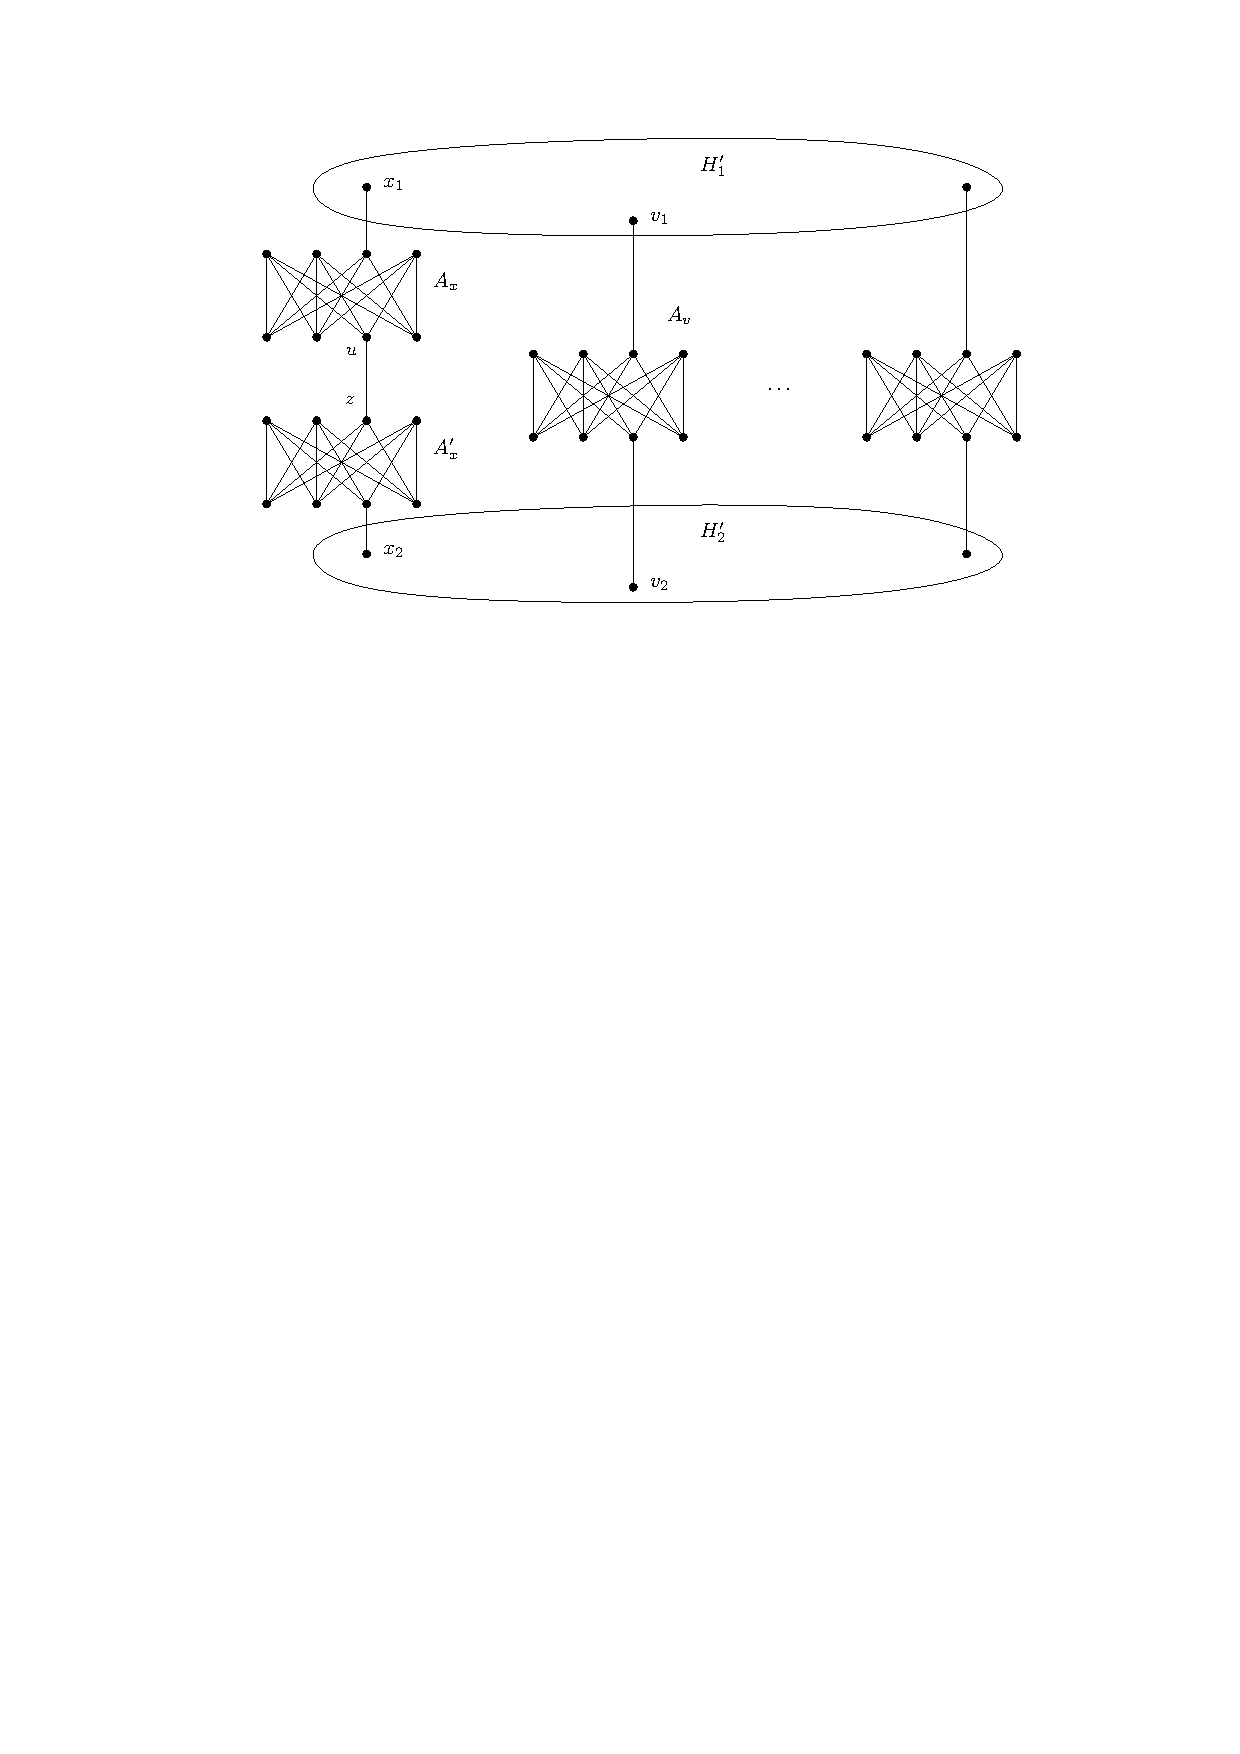
\includegraphics[scale=0.92]{chapter-6-NTP/hamilton-prime}
\caption{\lasse{Construction used in the proof of \cref{le:Ham-to-Ham}.}}
\label{fig_hamilton_cycle_lemma}
\end{figure}

\lasse{
For claim (i), assume that $H'$ has a Hamiltonian cycle $C'$. Then we obtain a Hamiltonian cycle $C$ in $H$ using the edge $\set{u,z}$ in the following fashion: We start at the vertex $u$, and traverse all the vertices of $A_x$ in such an order that we can proceed to go to $x_1$ afterwards. Now we follow the edges of the cycle $C'$, switching alternatingly between $H'_1$ and $H'_2$ after each edge. Precisely, whenever we follow an edge of $C'$ to encounter a new vertex $v_1$ in $H'_1$ ($v_2$ in $H'_2$, respectively), we traverse all the vertices of $A_v$ and go to $v_2$ ($v_1$, respectively) and then follow the next edge of $C'$. Because the graph $H'$ has an even number of vertices (it is bipartite and 3-regular), we will end up at $x_2$. We then complete the tour by traversing all vertices of $A'_x$ and going along the edge $\set{u,z}$ at the end. This describes a Hamiltonian cycle of $H$ which uses the edge $\set{u,z}$.
}

\lasse{
For claim (ii), we prove the contrapositive. Assume that $H$ has a Hamiltonian path $P = (w_1,\dots,w_n)$ starting at vertex $u$, we have to prove that $H'$ has a Hamiltonian cycle. Consider the second vertex $w_2$ on the path $P$. Note that if $w_2 = z$, then $w_n$ is in $A_x$. On the other hand, if $w_2$ is in $A_x$, then $w_n$ is in $A'_x$. We first assume that $w_2 \in A_x$ and $w_n \in A'_x$.
We claim that the Hamiltonian path $P$ necessarily switches between $H'_1$ and $H'_2$ after every of its edges in $H'_1$ or $H'_2$. Indeed, let $v \neq x$ be a vertex of $H'$ and assume without loss of generality that from the two vertices $v_1$ and $v_2$ the path $P$ first encounters $v_1$. If the path does not immediately switch to $v_2$, then it will at a later stage need to visit $v_2$. But in this case, it has to visit $A_v$ after visiting $v_2$, in contradiction to the fact that the path has to return to $A'_x$. This proves that $P$ switches between $H'_1$ and $H'_2$ after every egde in $H'_1$ or $H'_2$. Then looking at the edges of $P$ which lie in $H'_1$ or $H'_2$, we see that $H'$ has a Hamiltonian cycle. Finally, an analogous statement holds in the case $w_2 = z$. So we have proven the claim.  
}
\end{proof}


%%%%%%%%%%%%%%%%%

\begin{figure}[htpb]
\centering
 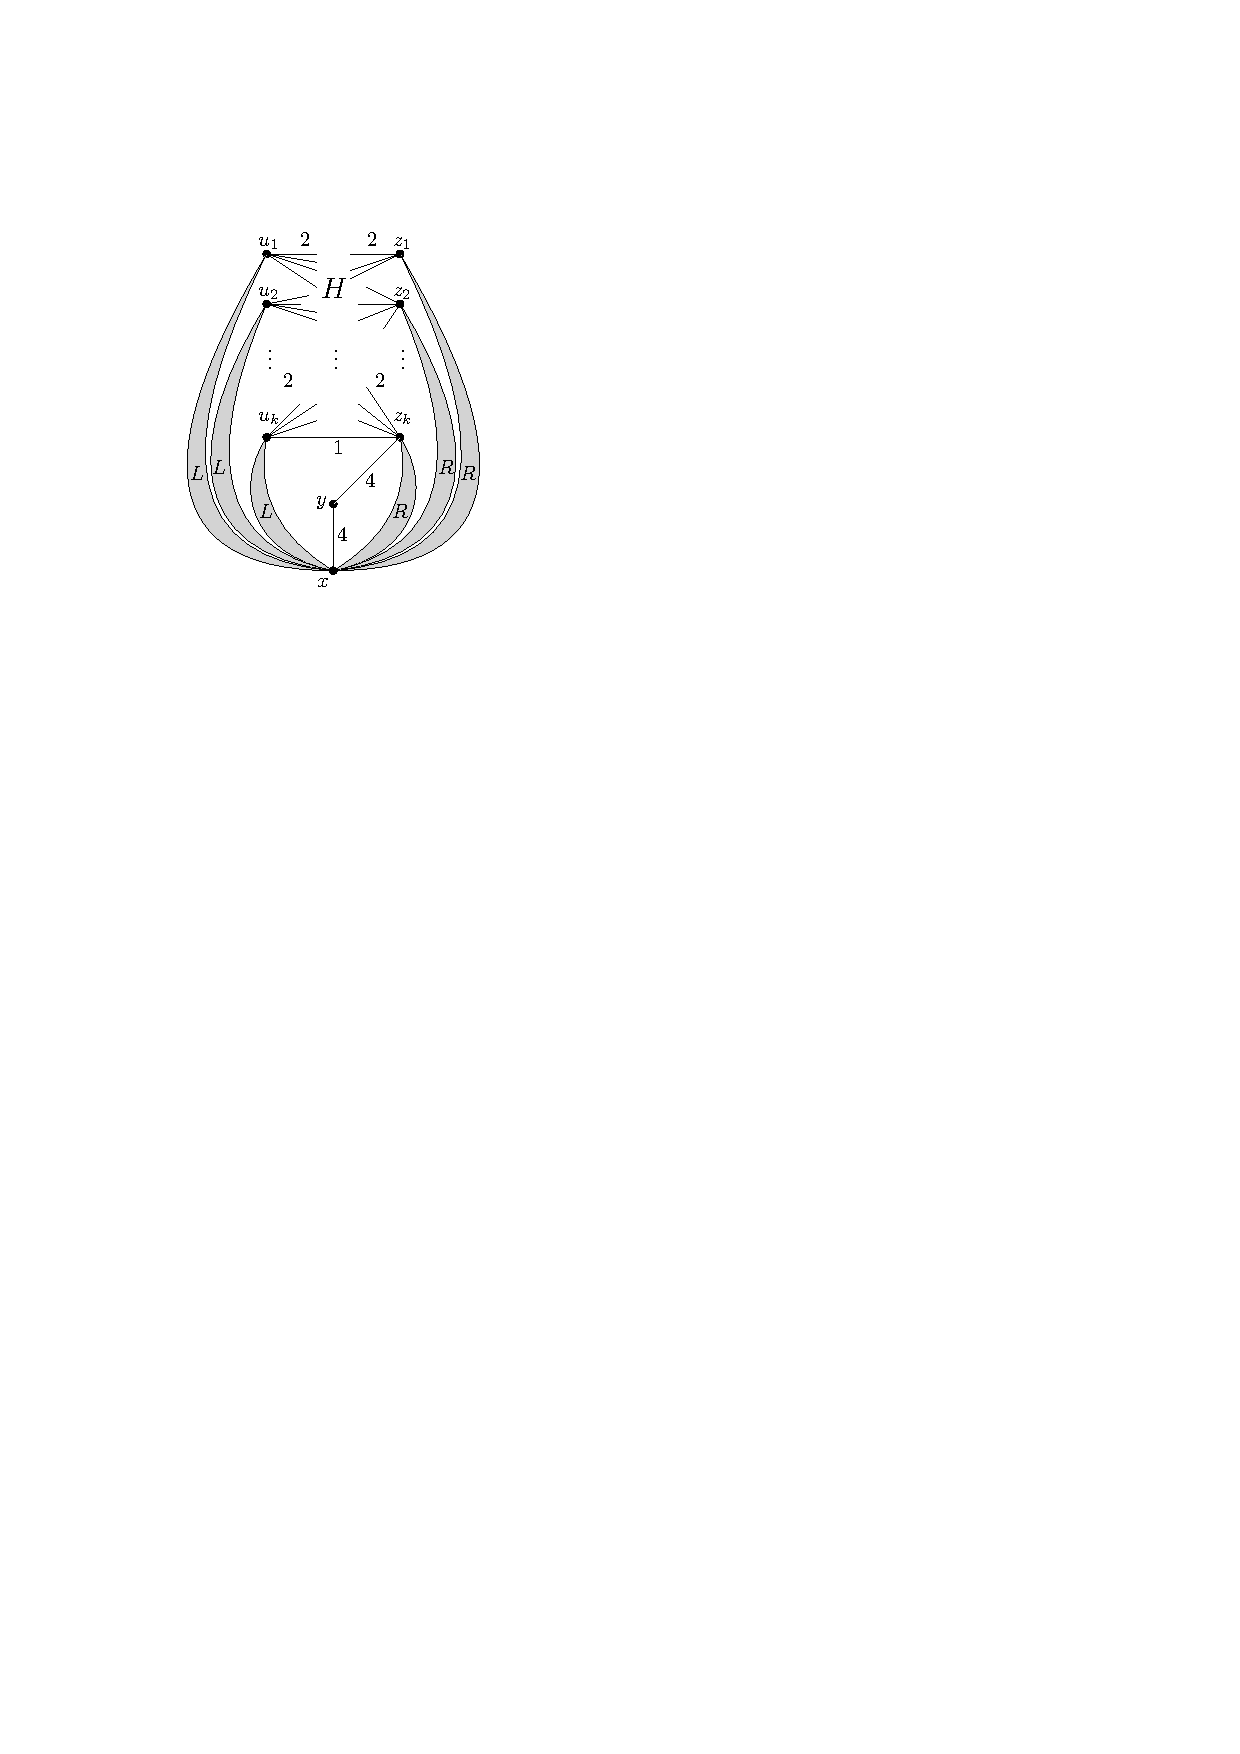
\includegraphics[scale=1.1]{chapter-6-NTP/act-hamilton-cycle-a}
\caption{Sketch of the {\xxxNTP} instance $(G, w)$ obtained from the 4-regular bipartite graph $H$.}
\label{fig:reduction-overview}
\end{figure}
Now let $H$ be a 4-regular bipartite graph as described in Lemma~\ref{le:Ham-to-Ham}.
Let $U=\fromto{u_1}{u_k}$ and $Z=\fromto{z_1}{z_k}$ denote the two parts in the bipartition of $H$, 
and let $\{u_k,z_k\}$ be its special edge.
We create an instance $(G,w)$ of {\xxxNTP} from $H$. An informal sketch of this instance $(G,w)$ is depicted in \cref{fig:reduction-overview}. Formally, it is described the following way:
The graph $G$ has the vertex set 
%%%%%%%%%%%%%%%%%
\[ 
V(G) =  \set{x, y} \cup U \cup Z 
        \cup \bigcup_{i=1}^k \fromto{v_{i1}}{v_{i4}} \cup \bigcup_{i=1}^k \set{v'_{i1}, v'_{i2}}.
\]
%%%%%%%%%%%%%%%%%
Furthermore, the graph $G$ has the following edges and edge weights:
\begin{itemize}
\item \lasse{Between the vertex sets $U$ and $Z$, the graph $G$ has exactly the same edges as the graph $H$. 
For every such edge $e$, we set} $w(e) = 2$, if $e \neq \set{u_k, z_k}$ and $w(\set{u_k, z_k}) = 1$.
\item For every $i = 1,\dots,k$, the induced subgraph $L_i = G[\set{x, u_i, v_{i1}, v_{i2}, v_{i3}, v_{i4}}]$ 
is called the \emph{$i$-th gadget of type L} and has edges and edge weights as depicted in \cref{fig:act-hamilton-cycle}.
\item For every $i = 1,\dots,k$, the induced subgraph $R_i = G[\set{x, z_i, v'_{i1}, v'_{i2}}]$ is called the 
\emph{$i$-th gadget of type R} and has edges and edge weights as depicted in \cref{fig:act-hamilton-cycle}.
\item Finally, the two edges $\set{x,y}$ and $\set{y, z_k}$ have $w(\set{x,y}) = w(\set{y, z_k}) = 4$. The induced subgraph $G[\set{x,y,z_k}]$ is called the \emph{gadget $C$}.
\end{itemize}
%%%%%%%%%%%%%%%%%%%%%%%%%%
\begin{figure}[htpb]
\centering
 
\includegraphics[scale=1.1]{chapter-6-NTP/act-hamilton-cycle-b-simplified}
\qquad\qquad\qquad
 
\includegraphics[scale=1.1]{chapter-6-NTP/act-hamilton-cycle-c}
\caption{Gadget of type $L$ (on the left) and gadget of type $R$ (on the right).}
\label{fig:act-hamilton-cycle}
\end{figure}
%%%%%%%%%%%%%%%%%%%%%%%%%%
Now assume that $(G, w)$ allows some schedule $\sigma$ of objective value 7. 
During any time slot $[t-1,t]$ with $1\le t\le7$, the $i$-th gadget of type $L$ will 
consist of either one or two connected components under schedule $\sigma$. 
If there is a single connected component, we say that $L_i$ is \emph{fully-connected} during the $t$-th time slot. If there are two connected components (one containing  $x$, and one containing $u_i$), we say that $L_i$ is \emph{semi-connected} during the $t$-th time slot. In the same manner, during the $t$-th time slot, gadget $R_i$ is either fully-connected or semi-connected with $x$ and $z_i$ in different components. Likewise, the gadget $C$ is either fully-connected, or semi-connected with $x$ and $z_k$ in different components.

\begin{lemma}
\label{lemma:gadgets_properties}
Let $(G,w)$ be the instance described above. 
Every schedule of objective value 7 for $(G, w)$ satisfies the following.
\begin{enumerate}[(i)]
\item A gadget of type $R$ is fully-connected during time slots 2 and 6, and 
semi-connected during each of the remaining five time slots.
\item For each $i=1,\dots,k$, there are $t_1,t_2 \in \set{1,2,4,6,7}$ with $t_1\ne t_2$, such that the gadget $L_i$ is fully-connected during time slots $3,5,t_1, t_2$, 
and semi-connected during each of the remaining three time slots.
\item The gadget $C$ is fully-connected during time slot 4, 
and semi-connected during each of the remaining six time slots.
\end{enumerate}
\end{lemma}
\begin{proof}
Note that the sum of all edge weights in $G$ is $8k-1 +32k +16k +8 = 56k+7 = 7(8k + 1) = 7(|V(G)|-1)$. 
This implies that each of the graphs $G_1,\ldots,G_7$ is a tree (in particular, it is acyclic) and that the activity interval of each edge is contained in $[0, \beta]$.
For the proof of (i), consider the vertex $v'_{i1}$ in the gadget $R_i$. 
There is exactly one time slot $[t-1, t]$ during which both edges incident to $v'_{i1}$ are active, 
and we have $t=2$ or $t=6$. 
Analogously, there is exactly one time slot $[t'-1, t']$ during which both edges incident to 
the vertex $v'_{i2}$ are active, and we have $t' = 2$ or $t' = 6$. 
As $t=t'$ yields the contradiction that $G_t$ has a cycle, we conclude $\set{t,t'}=\set{2,6}$ and (i) follows. 
Claims (ii) and (iii) can be proven in the same manner. 
\end{proof}

\begin{lemma}
\label{lemma:lasse-if}
Let the graph $H$ and the special edge $\set{u,z} \in E(H)$ be as described in \cref{le:Ham-to-Ham}, and let $(G, w)$ be the corresponding {\xxxNTP} instance. 
If $H$ contains a Hamiltonian cycle which uses the special edge, then $\ntp(G, w) \geq 7$.
\end{lemma}
\begin{proof}
Let $e_0 = \set{u, z} = \set{u_k, z_k}$ be the special edge. There is a Hamiltonian cycle $W$ using $e_0$. Then the graph $H-E(W)$ is 2-regular, hence there exist pairwise disjoint matchings $M_1, \ldots, M_4$ such that $M_1 \dotunion M_2 = E(W)$ and $M_3 \dotunion M_4 = E(H) - E(W)$ and $e_0 \in M_1$. We describe a schedule $\sigma$ with objective value 7:
\begin{itemize}
\item All gadgets of type $R$ are fully-connected during time slots 2 and 6, and semi-connected otherwise.
\item All gadgets of type $L$ are fully-connected during time slots 1, 3, 5, and 7, and semi-connected otherwise.
\item The gadget $C$ is fully-connected during time slot 4, and semi-connected otherwise.
\item All edges $e \in M_1 - \set{e_0}$ have activity interval $[2, 4]$. The edge $e_0$ has activity interval $[2, 3]$.
\item All edges $e \in M_2$ have activity interval $[3, 5]$.
\item All edges $e \in M_3$ have activity interval $[0, 2]$.
\item All edges $e \in M_4$ have activity interval $[5, 7]$.
\end{itemize}
It is easy to see that a schedule $\sigma$ with these properties does indeed exist. \cref{table:lasse-if} together with \cref{fig:one-page-if-overview} provides a schematic description of the schedule, by indicating for each number $t$, which edges are scheduled and which gadgets are fully connected during the the $t$-th time slot $[t-1, t]$.  Notice that the active edges in $H$ form a matching of $H$ during the time slots 1,2,3,5,6, and 7, 
and form a Hamiltonian path of $H$ during the time slot 4. 
By checking each of the cases $t=1,\dots,7$, it is easily seen that each of the graphs $G^\sigma_1,\ldots,G^\sigma_7$ is connected. We therefore conclude that $\ntp(\sigma) = 7$. 
\begin{table}[htpb]
\centering
 \begin{tabular}{ c | c | c | c | c | c | c } 
 \multicolumn{7}{c}{time slot}\\
	1 & 2 & 3 & 4 & 5 & 6 & 7 \\
	\hline
	 & $R$ & & & & $R$ & \\
	 $L$ & & $L$ & & $L$ &  & $L$ \\
	 & & & $C$ & & &  \\
	 & & $M_1$ & $M_1 - \set{e_0}$  & & &  \\
	  & & & $M_2$  & $M_2$ & &  \\
	  $M_3$ & $M_3$ & &  &  & &  \\
	   & & &  &  & $M_4$ & $M_4$ 
 \end{tabular}
 \caption{Description of the schedule $\sigma$ from \cref{lemma:lasse-if}.}
 \label{table:lasse-if}
\end{table}
%%%%%%%%%%%%%%%%%%%%%%%%%%
\begin{figure}[htpb]
\centering
 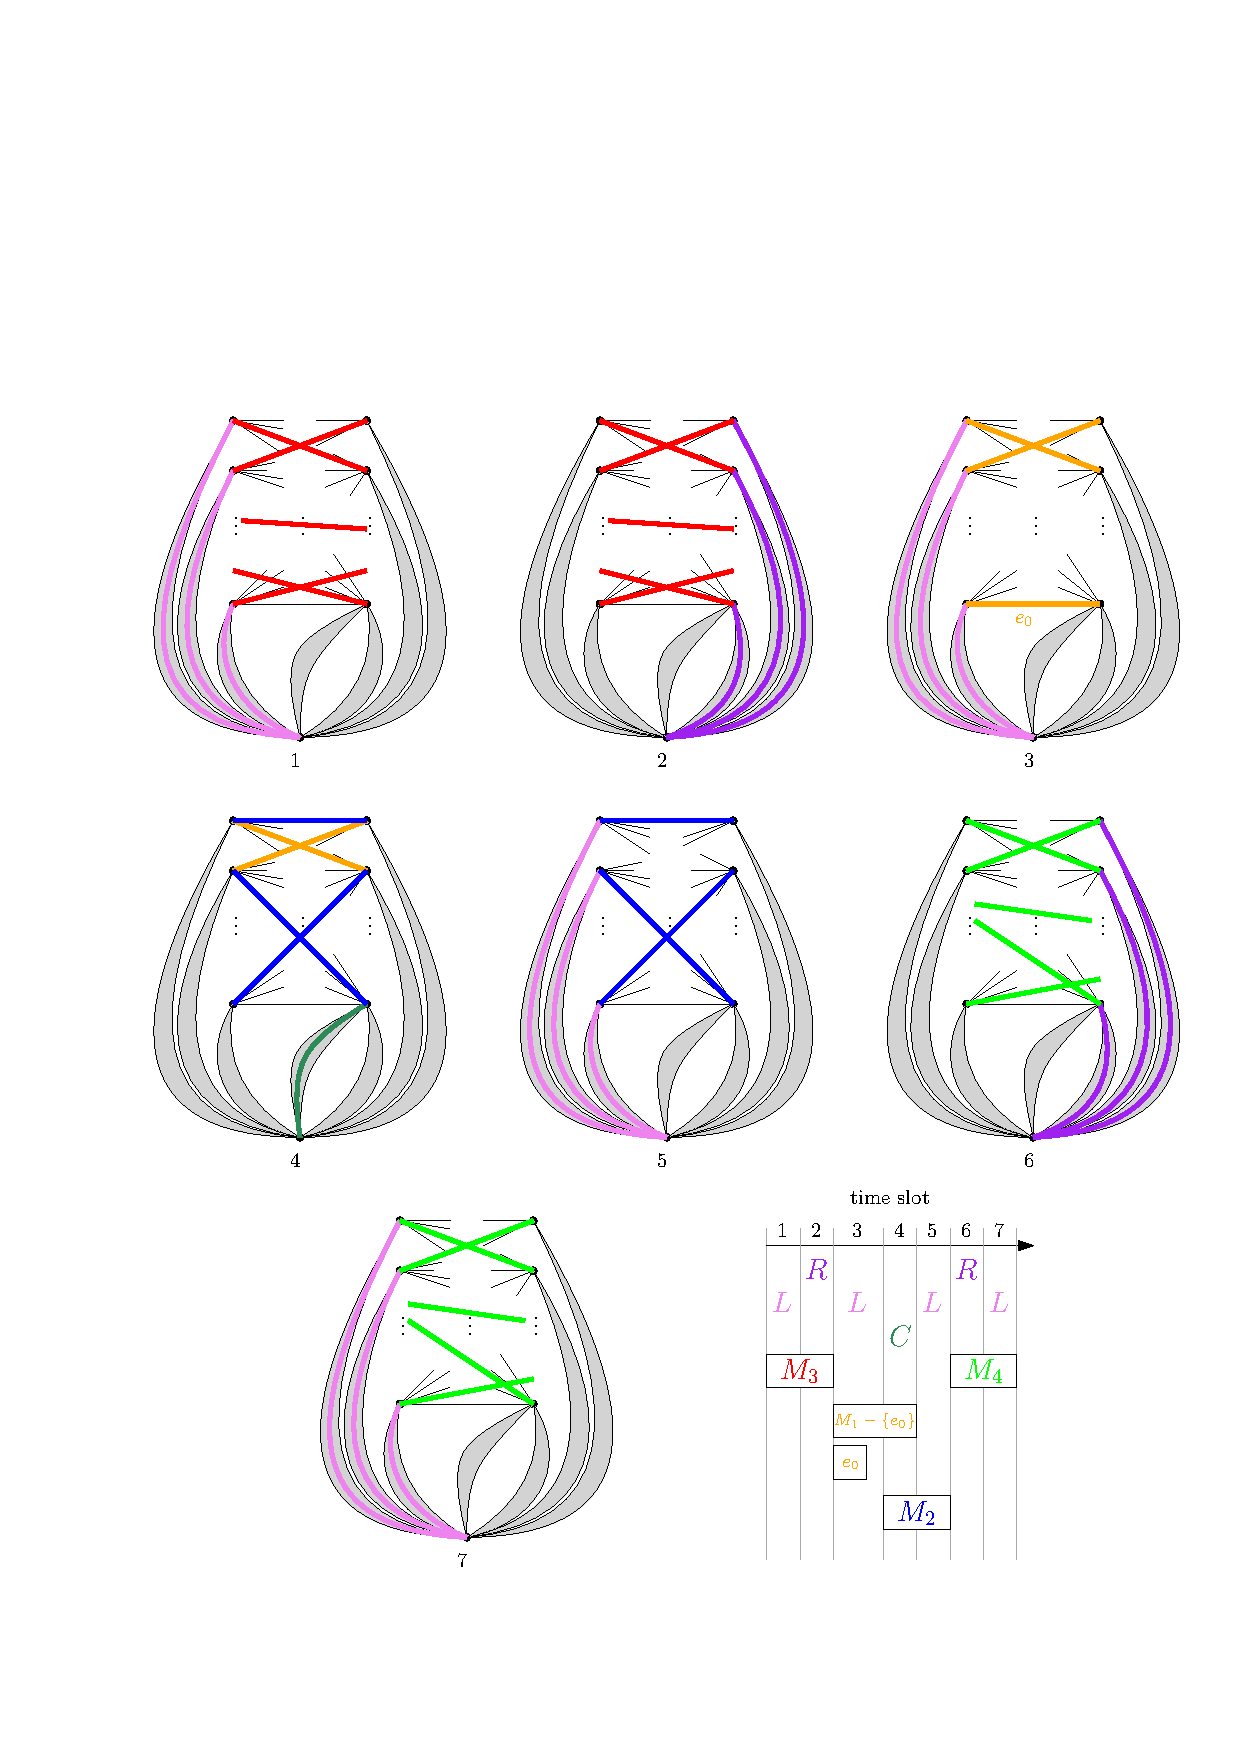
\includegraphics[width=0.95\textwidth]{chapter-6-NTP/toggle-one-page}
\caption{A visual demonstration of how the schedule described in \cref{lemma:lasse-if} and \cref{table:lasse-if} keeps the instance connected for seven time units. A colored figure is available online. Notice how during time slot 4, the edge set $M_1 \cup M_2 - \set{e_0}$ forms a Hamiltonian path in $H$. \cref{lemma:lasse-only-if} shows that this is unavoidable for any schedule $\sigma$ with $\ntp(\sigma) = 7$.}
\label{fig:one-page-if-overview}
\end{figure}
%%%%%%%%%%%%%%%%%%%%%%%%%%
 
\end{proof}

\begin{lemma}
\label{lemma:lasse-only-if}
Let the graph $H$ and the special edge $\set{u,z} \in E(H)$ be as described in \cref{le:Ham-to-Ham}, and let $(G, w)$ be the corresponding {\xxxNTP} instance. If $\ntp(G, w) \geq 7$, then $H$ contains a Hamiltonian path starting at vertex $u$.
\end{lemma}
\begin{proof}
So assume there exists a schedule $\sigma$ of objective value 7. 
For a vertex $v \in U \cup Z$, and $t \in \fromto{1}{7}$, let $d_t(v) = |\delta(v) \cap E(H) \cap E_t|$ denote the number of incident edges of $v$, which are both in $E(H)$ and active during the $t$-th time slot. The strategy of the proof will be to repeatedly deduce some conditions for $d_t(v)$. 
Let $e_0 = \set{u, z} = \set{u_k, z_k}$ be the special edge.

First, recall \cref{lemma:gadgets_properties}. Consider vertex $z_i$ for some $i \in \fromto{1}{k}$. We know that for each $t \in \set{1, 3, 5, 7}$ in the $t$-th time slot both the gadget $R_i$ and the gadget $C$ are semi-connected. But of course at least one edge incident to $z_i$ must be active during the $t$-th time slot. Hence $d_1(z_i), d_3(z_i), d_5(z_i), d_7(z_i) \geq 1$.  Note that the four edges in $\delta(z_i) \cap E(H)$ each have weight at most 2 (in the case $i \neq k$ we have four times weight 2, and for $i = k$ we have three times weight 2, and $w(e_0) = 1$). For the sake of contradiction, assume $d_1(z_i) > 1$. Then from the four edges in $\delta(z_i) \cap E(H)$ at least two are scheduled at time $0$. This is a contradiction to  $d_3(z_i), d_5(z_i), d_7(z_i) \geq 1$. Hence $d_1(z_i) = 1$. By the same argument, $d_7(z_i) = 1$. A similar argument shows that $e_0 \not\in E_4$.

Next, consider the graph $G_1$ of active edges in the first time slot. We know that  $d_1(z_i) = 1$ for all $i= 1,\dots, k$. Hence the induced subgraph $G_1[U \cup Z]$ on $2k$ vertices is acyclic, has $k$ edges, and therefore has $k$ connected components. But because $G_1$ is connected, and because all the gadgets of type $R$ and the gadget $C$ are semi-connected during time slot 1, this implies that every single gadget of type $L$ is actually fully-connected during time slot 1. The same argument holds for time slot 7. In total, together with \cref{lemma:gadgets_properties}, we have that a gadget of type $L$ is fully-connected during the $t$-th time slot, if and only if $t \in \set{1, 3, 5, 7}$. This in turn implies that for all $i = 1,\dots, k$, one has $d_2(u_i), d_4(u_i), d_6(u_i) \geq 1$. The two facts $d_2(u_i) \geq 1$ and $d_6(u_i) \geq 1$ together imply $d_4(u_i) \leq 2$. Likewise, for all $i = 1,\dots,k$, the two facts $d_1(z_i) = 1$ and $d_7(z_i) = 1$ together imply $d_4(z_i) \leq 2$.

Finally, we claim $d_4(u_k) = 1$. In fact, $d_4(u_k) = 0$ is impossible, because gadgets of type $L$ are semi-connected during time slot 4. For the sake of contradiction, assume $d_4(u_k) > 1$. We know that $d_2(u_k) \geq 1, d_6(u_k) \geq 1$ and $e_0 \not\in E_4$ and $w(e_0) = 1$. So our assumption $d_4(u_k) > 1$ is only possible if $e_0 \in E_2$ or $e_0 \in E_6$. But for the vertex $z_k$, we also know $d_1(z_k), d_3(z_k), d_5(z_k), d_7(z_k) \geq 1$. This is a contradiction to $e_0 \in E_2 \cup E_6$, hence our assumption was wrong and $d_4(u_k) = 1$.
In summary, during time slot 4, all gadgets of type $L$ and $R$ are semi-connected. We also have for all $i=1,\dots,k$ that $d_4(u_i) \leq 2$ and $d_4(z_i) \leq 2$. \lasse{Furthermore, we have} $d_4(u_k) = 1$. However, $G_4$ is connected. These facts together imply that the induced subgraph $G_4[U \cup Z]$ is a Hamiltonian path in $H$ starting at $u_k = u$.
\end{proof}

By combining \cref{le:Ham-to-Ham,lemma:lasse-only-if,lemma:lasse-if} we get
the following summarizing theorem.
%%%%%%%%%%%%%%%%%%%%%%%%%%
\begin{theorem}
\label{th:value=7}
For {\xxxNTP} it is strongly NP-hard to decide whether there exists a schedule
of objective value at least~$7$.
 
\end{theorem}
%%%%%%%%%%%%%%%%%%%%%%%%%%

All edge weights in the above reduction are in the set $\fromto{1}{7}$.
A minor modification yields the following corollary.
%%%%%%%%%%%%%%%%%%%%%%%%%%
\begin{restatable}{corollary}{weightsOneToSix}
\label{coro:small-weights}
Problem {\xxxNTP} is strongly NP-hard, even if all edge weights are in $\fromto{1}{6}$.
\end{restatable}
\begin{proof}
Edges of weight~$7$ only show up in the gadget of type $L$.
Figure~\ref{fig_hamilton_cycle_improved} shows a modified version of this gadget that emulates 
the edges of weight~$7$ by edges with weights in $\fromto{1}{6}$.
One easily verifies that the functionality of the gadget remains the same and that in particular
Lemma~\ref{lemma:gadgets_properties} still holds true.
\end{proof}
%%%%%%%%%%%%%%%%%%%%%%%%%%
%%%%%%%%%%%%%%%%%%%%%%%%%%
\begin{figure}[htpb]
\centering

\includegraphics[scale=1.1]{chapter-6-NTP/act-hamilton-cycle-b}
\caption{The modified version of the type $L$ gadget without edges of weight $7$.}
\label{fig_hamilton_cycle_improved}
\end{figure}
%%%%%%%%%%%%%%%%%%%%%%%%%%

As it is NP-hard to distinguish between {\xxxNTP} instances with optimal objective value~$6$ 
and {\xxxNTP} instances with optimal objective value~$7$, we also get the following 
in approximability result.
%%%%%%%%%%%%%%%%%%%%%%%%%%
\begin{corollary}
\label{coro:inapproximability}
Unless P=NP, there is no polynomial time approximation algorithm for {\xxxNTP} with
worst case guarantee better than $7/6$.
 
\end{corollary}
%%%%%%%%%%%%%%%%%%%%%%%%%%


%%%%%%%%%%%%%%%%%%%%%%%%%%%%%%%%%%%%%%%%%%%%%%%%%%%%%%%%%%%%%%%%%%%%%%%%%
%%%%%%%%%%%%%%%%%%%%%%%%%%%%%%%%%%%%%%%%%%%%%%%%%%%%%%%%%%%%%%%%%%%%%%%%%
\section{A positive result for objective value three}
\label{sec:value-three}
%%%%%%%%%%%%%%%%%%%%%%%%%%%%%%%%%%%%%%%%%%%%%%%%%%%%%%%%%%%%%%%%%%%%%%%%%
In Section~\ref{sec:value-seven}, we have established the NP-hardness of deciding whether 
there exists a schedule of objective value at least~$7$. 
As a complementary result, we now show that it can be decided in polynomial time whether there is
a schedule of objective value at least~$3$.

%%%%%%%%%%%%%%%%%%%%%%%%%%
\begin{theorem}
\label{th:value=3}
For an instance of {\xxxNTP} on a graph with $m$ edges, it can be decided in $\bigO(m^3)$ time 
whether $\ntp(G,w)\ge3$.
\end{theorem}
%%%%%%%%%%%%%%%%%%%%%%%%%%
\begin{proof}
Let $G=(V,E)$. 
We partition the edge set $E$ into set $W_1$ (edges of weight~$1$), set $W_2$ (edges of weight~$2$),
and set $W_{\ge3}$ (edges of weight at least~$3$).
In a schedule of objective value $3$, we may activate all edges in $W_{\ge3}$ at time~$0$.
We interpret an edge in $W_2$ as a pair of two edges of weight $1$: one of these two edges is scheduled 
during the middle time slot $[1, 2]$; the other edge can either be scheduled during slot $[0,1]$ 
or during slot $[2,3]$. 
Edges in $W_1$ are scheduled during one of the three slots $[0,1]$, $[1,2]$, $[2,3]$.

By Lemma~\ref{le:structure}, we may assume that in a feasible schedule of length~$3$ the 
graphs $(V,E_t)$ with $t=1,2,3$ are trees.
Let $H_3$    be the graph that results from $G$ after contracting the edge set $W_{\ge3}$, and
let $H_{23}$ be the graph that results from $G$ after contracting the edge set $W_2\cup W_{\ge3}$.
We introduce three matroids:
\begin{itemize}
\item The matroid $\mathcal{F}_1$ has the ground set $W_1\cup W_2$. 
A set $F\subseteq W_1\cup W_2$ is independent in $\mathcal{F}_1$, if and only if $F$ is acyclic in graph $H_3$.
\item The matroid $\mathcal{F}_2$ has the ground set $W_1$.
A set $F\subseteq W_1$ is independent in $\mathcal{F}_2$, if and only if $F$ is acyclic in graph $H_{23}$.
\item The matroid $\mathcal{F}_3$ has ground set $W_1\cup W_2$, and coincides with $\mathcal{F}_1$.
\end{itemize}
\lasse{Recall that a base of a matroid is a maximal independent set. By construction, the bases of $\mathcal{F}_1, \mathcal{F}_2$ and $\mathcal{F}_3$ have the following properties. (A small technicality we have to consider is that $W_2$ and $W_{\geq3}$ may contain cycles.)}
\lasse{
\begin{itemize}
\item If a set $F \subseteq W_1 \cup W_2$ is independent in the matroid $\mathcal{F}_1$, then $F$ is a base of $\mathcal{F}_1$ if and only if $F$ induces a spanning tree of $H_3$ if and only if $F \cup W_{\geq 3}$ contains a spanning tree of $G$.
\item If a set $F \subseteq W_1$ is independent in the matroid $\mathcal{F}_2$, then $F$ is a base of $\mathcal{F}_2$ if and only if $F$ induces a spanning tree of $H_{23}$ if and only if $F \cup W_2 \cup W_{\geq 3}$ contains a spanning tree of $G$.
\item If a set $F \subseteq W_1 \cup W_2$ is independent in the matroid $\mathcal{F}_3$, then $F$ is a base of $\mathcal{F}_3$ if and only if $F$ induces a spanning tree of $H_3$ if and only if $F \cup W_{\geq 3}$ contains a spanning tree of $G$.
\end{itemize}
}

\lasse{Now observe that scheduling an edge of weight 1 is equivalent to choosing in which of the three time slots 1,2 or 3 it is scheduled. Scheduling an edge 2 is equivalent to always schedule it in time slot 2 and choose whether it is scheduled in time slot 1 or 3. From these facts together with \cref{le:structure}, we can deduce that we can connect the graph during time slots 1,2 and 3 (that is $\ntp(G,w)\ge3$ holds)}, if and only if there exist three pairwise disjoint subsets
$S_1,S_2,S_3$ of $W_1 \cup W_2$, such that $S_t$ forms a base of the matroid $\mathcal{F}_t$ for $t=1,2,3$.
This can be checked in $\bigO(m^3)$ time by using Edmond's matroid partitioning algorithm \cite{edmonds1965minimum}.
\end{proof}

By a similar (but simpler) argument we can also decide in polynomial time whether $\ntp(G,w)\ge2$.
Deciding whether $\ntp(G,w)\ge1$ is trivial.
The complexity of deciding whether $\ntp(G,w)\ge\beta$ remains open for $\beta\in\{4,5,6\}$.


%%%%%%%%%%%%%%%%%%%%%%%%%%%%%%%%%%%%%%%%%%%%%%%%%%%%%%%%%%%%%%%%%%%%%%%%%
%%%%%%%%%%%%%%%%%%%%%%%%%%%%%%%%%%%%%%%%%%%%%%%%%%%%%%%%%%%%%%%%%%%%%%%%%
\section{The Greedy algorithm}
\label{sec:greedy}
%%%%%%%%%%%%%%%%%%%%%%%%%%%%%%%%%%%%%%%%%%%%%%%%%%%%%%%%%%%%%%%%%%%%%%%%
We introduce a greedy algorithm that maintains connectivity by always
activating edges of the largest possible weight.
Formally, we let $F_t\subseteq E_t$ denote the set of edges whose activity intervals 
end at time $t$.
By $U_t=E-(E_1\cup E_2\cup\cdots\cup E_t)$ we denote the set of edges that have not been 
used and activated before time $t$.

Now the {\greedy} algorithm starts its work by initializing 
$E_0:=\emptyset$, $F_0:=\emptyset$, and $U_0:=E$.
For $t\ge0$, the set $E_{t+1}$ for time slot $[t,t+1]$ is computed as follows.
If the graph $(V,E_t-F_t)$ is a tree, we set $E_{t+1}:=E_t$.
If the graph $(V,E_t-F_t)$ is a forest with $c$ components, we turn it into 
a tree by adding a maximum weight subset $A\subseteq U_t$ of cardinality $c-1$;
then we set $E_{t+1}:=(E_t-F_t)\cup A$.
In case no such set $A$ exists, the {\greedy} algorithm terminates.
(The set $A$ can be computed for instance by applying Kruskal's algorithm for 
maximum spanning trees; ties are broken arbitrarily.)

%%%%%%%%%%%%%%%%%
\begin{theorem}
\label{th:greedy.approx}
For every graph $G=(V,E)$ on $n$ vertices and for every $w:E\to\NN_0$, 
the {\greedy} algorithm computes a schedule of length at least $\ntp(G,w)/(n-1)$.
Furthermore, there exist instances on which the schedule computed by the 
{\greedy} algorithm is a factor $\lfloor n/2\rfloor$ below the optimal objective value.
\end{theorem}
%%%%%%%%%%%%%%%%%
\begin{proof}
For the positive result, we consider the time slot $[T,T+1]$ at which {\greedy} terminates.
Then the graph $(V,(E_T-F_T)\cup U_T)$ is not connected.
We consider the vertex set $C\subseteq V$ of one of the components of that graph, and the
corresponding edge cut $\delta(C)$.
Then the weight $w(\delta(C))=\sum_{e\in\delta(C)}w(e)$ yields a trivial upper bound for the 
optimal objective value: 
%%%%%%%%%%%%%%%%%
\begin{equation}
\label{eq:greedy}
\ntp(G,w) ~\le~ w(\delta(C))
\end{equation}
%%%%%%%%%%%%%%%%%
Since every edge set $E_j$ with $1\le j\le T$ induces a tree, we have $|E_j|=n-1$ and hence
$|E_j\cap \delta(C)|\le n-1$.
As all edges in the cut $\delta(C)$ have been activated and run to completion before the 
time slot $[T,T+1]$, we conclude $T\ge w(\delta(C))/(n-1)$, which together with \eqref{eq:greedy}
yields the desired approximation guarantee.

For the negative result, we consider the complete graph $K_n=(V,E)$ on $n$ vertices with 
weights $w(e)=1$ for all $e\in E$.
A folklore result (see for instance Palmer~\cite{Palmer2001}) says that the maximum number of 
edge-disjoint spanning trees that can be packed into $K_n$ is $\lfloor n/2\rfloor$.
This implies $\ntp(K_n,w)=\lfloor n/2\rfloor$.
On the other hand, if the {\greedy} algorithm at time $0$ activates the $n-1$ edges in the edge
cut $\delta(v)$ for some $v\in V$, the objective value of the resulting schedule equals~$1$.
\end{proof}


%%%%%%%%%%%%%%%%%
\begin{theorem}
\label{th:greedy.cactus}
For every connected graph $G=(V,E)$, the following two statements are equivalent.
\begin{enumerate}[(i)]
\item $G$ is a cactus graph.
\item For every choice $w:E\to\NN_0$ of edge weights, the {\greedy} algorithm 
solves the {\xxxNTP} instance $(G,w)$ to optimality.
\end{enumerate}
\end{theorem}
%%%%%%%%%%%%%%%%%
%%%%%%%%%%%%%%%%%%%%%%%%%%%%%%%%%%%%%%%%%
\begin{figure}[tbh]
\begin{center}
\begin{tikzpicture}[scale=0.90]

\coordinate (p1) at (-1.5, 0.000);
\coordinate (p2) at ( 0.0, 1.732);
\coordinate (p3) at ( 1.5, 0.000);
\coordinate (p4) at ( 0.0,-1.732);
\foreach \x in {1,...,4}{\fill (p\x) circle (0.08);}

\node at ($(p1)+(-0.5, 0.00)$) {\large $v_1$};
\node at ($(p2)+(+0.5, 0.20)$) {\large $v_2$};
\node at ($(p3)+(+0.5,-0.30)$) {\large $v_3$};
\node at ($(p4)+(+0.5, 0.00)$) {\large $v_4$};

\draw[thick] (p1)--(p2)--(p3)--(p4)--(p1)--(p3);
\node at ($(p1)!0.5!(p2)+(-0.35, 0.1)$) {\large $3$};
\node at ($(p1)!0.5!(p4)+(-0.45, 0.0)$) {\large $2$};
\node at ($(p1)!0.5!(p3)+( 0.00, 0.4)$) {\large $1$};
\node at ($(p2)!0.5!(p3)+(+0.35, 0.1)$) {\large $1$};
\node at ($(p4)!0.5!(p3)+(+0.45, 0.0)$) {\large $2$};
\end{tikzpicture}
\end{center}
\caption{An instance $(H,w_H)$ on which the {\greedy} algorithm fails.}
\label{fig:cactus}
\end{figure}
%%%%%%%%%%%%%%%%%%%%%%%%%%%%%%%%%%%%%%%%%
\begin{proof}
We first show that (i) implies (ii).
Since cut-vertices split an {\xxxNTP} instance into smaller instances that do not interact 
with each other, it is sufficient to prove the statement for two-connected cactus graphs.
Hence we will assume that $G$ is a cycle on $n$ vertices, and we let $e_1,\ldots,e_n$ 
denote the edges in the cycle ordered by increasing weight so that 
$w(e_1)\le w(e_2)\le\cdots\le w(e_n)$.
It is easily seen that the optimal objective value for $(G,w)$ equals 
$\min\{w(e_1)+w(e_2),\,w(e_3)\}$.
As the {\greedy} algorithm activates the $n-1$ edges $e_2,\ldots,e_n$ at time~$0$ and 
activates the final edge $e_1$ at time $w(e_2)$, it yields the optimal objective value.

In order to show that (ii) implies (i), we first consider the graph $H$ on the four
vertices $v_1,v_2,v_3,v_4$ and the edge weights $w_H$ depicted in Figure~\ref{fig:cactus}.
As the {\greedy} algorithm at time~$0$ activates the three edges $\{v_1,v_2\}$, $\{v_1,v_4\}$, 
$\{v_3,v_4\}$ (that carry the weights $3,2,2$, respectively), at time~$2$ there remains no 
further possibility of connecting vertex $v_4$ to the rest of the graph; hence {\greedy} 
generates a schedule of value~$2$.
On the other hand, the optimal schedule results by activating the three edges $\{v_1,v_2\}$, 
$\{v_1,v_3\}$, $\{v_3,v_4\}$ at time~$0$, by activating edge $\{v_1,v_4\}$ at time~$1$,
and by activating edge $\{v_2,v_3\}$ at time~$2$; the corresponding optimal objective
value is $\ntp(H,w_H)=3$.
Hence {\greedy} fails to solve this instance $(H,w_H)$ to optimality.

Now let $G=(V,E)$ be an arbitrary connected graph that is not a cactus. 
This implies that $G$ does contain a subdivision $(V',E')$ of the four-vertex 
graph $H=(V_H,E_H)$ in Figure~\ref{fig:cactus}.
Let $E''\subseteq E$ be a subset of cardinality $|V-V'|$, so that the graph $(V,E'\cup E'')$
is connected.
We construct edge weights $w:E\to\NN_0$ as follows.
For every edge $e\notin E'\cup E''$ we set $w(e)=0$, and
for every edge $e\in E''$ we set $w(e)=3$.
Finally, we fix the weights $w(e)$ of the edges $e\in E'$ so that they emulate the 
weights $w_H:E_H\to\NN_0$ in the four-vertex graph $H$; if an edge $e\in E'$ belongs to the 
subdivision of some edge $f\in E_H$, we define $w(e)=w_H(f)$.
It is easily verified that the resulting instance $(G,w)$ satisfies $\ntp(G,w)=3$,
whereas the {\greedy} algorithm only yields an objective value of~$2$.
\end{proof}


%%%%%%%%%%%%%%%%%%%%%%%%%%%%%%%%%%%%%%%%%%%%%%%%%%%%%%%%%%%%%%%%%%%%%%%%%
%%%%%%%%%%%%%%%%%%%%%%%%%%%%%%%%%%%%%%%%%%%%%%%%%%%%%%%%%%%%%%%%%%%%%%%%%
\section{Parameterized complexity}
\label{sec:parameterized}
%%%%%%%%%%%%%%%%%%%%%%%%%%%%%%%%%%%%%%%%%%%%%%%%%%%%%%%%%%%%%%%%%%%%%%%%%
In this section, we show that problem {\xxxNTP} is fixed parameter tractable with 
respect to various parameters. \lasse{As the problem is already NP-hard even for highly restricted graphs,
we can only hope for positive parameterized complexity results for quite restricitive graph parameters,
or when additionally the edge weights are restricted.}
Note that Theorems~\ref{thm:hardness_complete_bipartite} and \ref{th:value=7} imply the NP-hardness 
of problem {\xxxNTP}, even if either the treewidth or the edge weights are bounded by a constant. 

\begin{restatable}{theorem}{fptBoundedWeightAndTW}
\label{th:fpt_weights_and_tw_bounded}
%If both the treewidth and the maximum edge weight of the input graph $G = (V, E)$ are bounded \lasse{by a constant integer $k$}, problem {\xxxNTP} \lasse{can be solved in $\bigO(|E|)$ time. The algorithm is fixed parameter tractable with respect to $k$}. 
\lasse{Problem {\xxxNTP} is fixed parameter tractable with respect to $w_{\max} + t$, where $w_{\max}$ is the maximum edge weight and $t$ the treewidth of the input graph.}
\end{restatable}
\begin{proof}
As the graph $G=(V,E)$ has treewidth $t$, there is a vertex $v\in V$ of degree at most $t$ \lasse{(here we use the property that $G$ is a simple graph, that is, it has no parallel edges.)}.
As every edge incident to $v$ has weight at most $w_{\max}$, we conclude $\ntp(G,w)\le w_{\max}^2$. 
For every $T=1,\ldots,w_{\max}^2$, we construct a formula $\Phi_T$ in monadic second-order 
graph logic $\text{MSO}_2$, so that $\Phi_T$ is satisfiable if and only if there exists a schedule 
of objective value at least $T$. 
We introduce Boolean variables $x_{e,t}$ for every $e\in E$ and every $t\in \{1,\dots,T\}$
to denote whether $e\in E_t$. 
The following statement can be formulated in $\text{MSO}_2$ by routine methods \lasse{(see for example \cite[chapter 7.4]{cygan2015parameterized})}:
\begin{align*}
\exists \sigma: E\to\{0,\ldots,&T\} ~~\forall e\in E ~~\forall t\in\{1,\ldots,T\}: \\
& x_{e,t} \iff \left(\sigma(e) < t \leq \sigma(e) + w(e)\right)\\
& \land \forall t\in\{1,\ldots,T\}: \set{e\in E \mid x_{e,t}} \text{ is a spanning tree.}
\end{align*}
Now Courcelle's theorem \cite{courcelle1990monadic} implies that the satisfiability of $\Phi_T$ 
can be checked in linear time for every $T=1,\ldots,w_{\max}^2$.
 
\end{proof}

\begin{restatable}{theorem}{exactAlgoExponential}
\label{th:exact}
On input graphs $G=(V,E)$, problem {\xxxNTP} is solvable in exponential time $\bigO(|E|^2\cdot|E|!)$. 
\end{restatable}
\begin{proof}
By Lemma~\ref{le:structure}, we may assume that in an optimal schedule $\sigma$ of length $T$ 
all graphs $G_1^\sigma, \dots, G_T^\sigma$ are trees.
As these trees are uniquely determined by the ordering in which $\sigma$ activates the edges,
we only need to check and evaluate $|E|!$ cases.
Each case is easily checked and evaluated in $\bigO(|E|^2)$ time.
 
\end{proof}

\begin{restatable}{theorem}{fptFeedbackEdge}
\label{thm:FPT_feedback_edge_set}
Problem {\xxxNTP} is fixed parameter tractable with respect to the size $k$ of a feedback edge set. 
There is a kernel with $\bigO(k)$ vertices and edges. 
\end{restatable}
\begin{proof}
Note that the input graph $G=(V,E)$ satisfies $|E|\le|V|-1+k$.
We first prove an auxiliary observation on the largest edge weight $w_{\max}$ in the graph:
We claim that $|V|\ge k+2$ implies $\ntp(G,w)\le w_{\max}$. 
Consider an optimal schedule as in Lemma~\ref{le:structure}, so that $|E_1|=|V|-1$.
As every edge in $E_1$ is certainly inactive from time $w_{\max}$ onwards, there remain at most 
$|E|-|E_1|=|E|-|V|+1\le k$ edges that could become active during the next time slot $[w_{\max},w_{\max}+1]$.
As a spanning tree needs at least $|V|-1\ge k+1$ edges, this proves the auxiliary observation.
As a consequence we get that in an optimal schedule an edge with weight $w_{\max}$ without loss 
of generality may be activated at time~$0$.

Now the kernelization procedure is clear:
As long as $|V|\ge k+2$ holds, we contract an edge with largest edge weight.
Note that the contraction maintains the inequality $|E|\le|V|-1+k$.
The resulting kernel satisfies $|V|\le k+1$ and $|E|\le2k$.
 
\end{proof}


The last theorem of this section shows that problem {\xxxNTP} is tractable on instances that in 
a certain sense are close to the preemptive tree packing problem of Nash-Williams. 
%%%%%%%%%%%%%%%%%%
\begin{restatable}{theorem}{fptAlmostAllWeightOne}
\label{th:fpt_almost_all_weight_one}
Let $(G,w)$ be an instance of {\xxxNTP} on $m$ edges, so that $m-k$ edges have weight~$1$ and 
the remaining $k$ edges have weight at most $k$. 
Then an optimal solution can be found in $\bigO(k^{2k}m^3)$ time.
\end{restatable}
%%%%%%%%%%%%%%%%%%
\begin{proof}
Let $E'=\set{e\in E: w(e)\ne1}$. 
For a schedule $\sigma$ of objective value $T$, we denote by $D_\sigma= \set{t: E_t^\sigma\cap E'\ne\emptyset}$ 
the set of time slots $[t-1,t]$ during which at least one edge of $E'$ is active. 
For every $t\le T$ with $t\notin D_\sigma$, graph $G_t=(V,E_t)$ is a connected graph in which 
all edges have weight 1.  
For each such $t$ with $t \not\in D_\sigma$, we introduce another schedule $\pi$, where the edge set $E_t$ is scheduled in the last time 
slot $[T-1, T]$ instead of the $t$-th time slot, and all edges activated during $[t, T]$ are activated 
one time unit earlier instead. Formally, schedule $\pi$ is such that
%%%%%%%%%%%%%%%%%%
\[(G^\pi_1,\dots, G^\pi_T) = (G^\sigma_1, \dots G^\sigma_{t-1}, G^\sigma_{t+1}, \dots, G^\sigma_T, G^\sigma_t). \]
%%%%%%%%%%%%%%%%%%
Observe that $\pi$ is also a schedule of objective value $T$. 
By repeating this procedure often enough, we conclude that there always exists an optimal schedule $\sigma$ so that $D_\sigma \subseteq \fromto{1}{k^2}$. 
Due to \cref{le:structure}, we can additionally require that each of $G_1, \dots, G_T$ is acyclic.

Therefore, the following is an algorithm to solve problem {\xxxNTP}: 
Iterate over all possible $k^{2k}$ choices of $(\sigma(e))_{e \in E'} \in \fromto{1}{k^2}^k$. 
For each fixed choice, the only edges left to schedule are edges of weight one. 
This can be done optimally the following way: 
For $t = 1,\dots, k^2$, let $W_t = \set{e \in E' : \sigma(e) < t \leq \sigma(e) + w(e)}$ be the set of edges in $E'$, which are active during the $t$-th time slot. 
If some $W_t$ has a cycle, we immediately skip to the next choice of $(\sigma(e))_{e \in E'}$. 
Otherwise, consider the matroid $\mathcal{F}_t = \set{F \subseteq E(G)-E' : W_t \cup F \text{ is acyclic}}$. 
We extend the definition of $\mathcal{F}_t$ to $t > k^2$ by setting $W_t = \emptyset$ in this case. 
The matroid $\mathcal{F}_t$ is isomorphic to the graphic matroid of $G$ after contracting each connected 
component of $W_t$ to a single vertex. 
Now we run Edmond's Matroid Partitioning algorithm \cite{edmonds1965minimum} to determine the 
maximal $T'\in\NN_0$ such that $E(G)-E'$ contains disjoint sets $F_1, \dots, F_{T'}$ such that $F_t$ 
is a base of $\mathcal{F}_t$ for all $t \in \fromto{1}{T'}$ (that is, we solve the problem of packing as 
many bases as possible into a matroid). 
As Edmond's Matroid Partitioning algorithm runs in $\bigO(m^3)$ time, the claimed time complexity follows.
\end{proof}


%%%%%%%%%%%%%%%%%%%%%%%%%%%%%%%%%%%%%%%%%%%%%%%%%%%%%%%%%%%%%%%%%%%%%%%%%
%%%%%%%%%%%%%%%%%%%%%%%%%%%%%%%%%%%%%%%%%%%%%%%%%%%%%%%%%%%%%%%%%%%%%%%%%


%%%%%%%%%%%%%%%%%%%%%%%%%%%%%%%%%%%%%%%%%%%%%%%%%%%%%%%%%%%%%%%%%%%%%%%%%
%%%%%%%%%%%%%%%%%%%%%%%%%%%%%%%%%%%%%%%%%%%%%%%%%%%%%%%%%%%%%%%%%%%%%%%%%
\section{Conclusion}
\label{sec:conclusion}
%%%%%%%%%%%%%%%%%%%%%%%%%%%%%%%%%%%%%%%%%%%%%%%%%%%%%%%%%%%%%%%%%%%%%%%%%
We have analyzed the computational complexity and the algorithmic behavior of non-preemptive
tree packing.
The problem is strongly NP-hard even on highly structured and extremely simple graph classes,
and we only have a handful of positive results.

There remain many open questions.
~(Q1) We have shown that {\xxxNTP} can be approximated in polynomial time within a factor of $n-1$, 
and that no approximation factor better than $7/6$ is possible (unless P=NP).
Where is the true approximation threshold?
In particular, we would like to know whether our problem allows a polynomial time approximation
algorithm with some constant worst case guarantee.
A major step towards an answer might be the analysis of the gap between the non-preemptive optimum 
and the polynomially computable preemptive optimum.
~(Q2) If all edge weights are equal to~$1$, problem {\xxxNTP} coincides with the preemptive problem 
version and hence is polynomially solvable.
On the other hand the problem is NP-hard, if all edge weights are in $\fromto{1}{6}$. 
What is the complexity of {\xxxNTP}, if all edge weights are in $\{1,2\}$?
~(Q3) The problem of deciding whether $\ntp(G,w)\ge\beta$ is polynomially solvable for 
every $\beta\le3$ and NP-hard for every $\beta\ge7$.
What is the complexity of this question for $\beta\in\{4,5,6\}$?




%--- BIBLIOGRAPHY --------------------------------------------------------------

% Print bibliography and include it in the table of contents:
%\printbibliography[heading=bibintoc]
\bibliographystyle{abbrv}
\bibliography{phd-wulf-literature}

\end{document}
